\documentclass{ttuthes2007}

%%%%%%%%%%%%%%%%%%%%%%%%%%%%%%%%%%%%%%%%%%%%%%
%Include any other add-on  packages you need:%
%%%%%%%%%%%%%%%%%%%%%%%%%%%%%%%%%%%%%%%%%%%%%%
\usepackage{amsmath,graphicx,bm,mathtools}
\usepackage[utf8]{inputenc}
\usepackage[T1]{fontenc}
\usepackage{lmodern}
\usepackage[labelfont=bf,labelsep=period]{caption}
\usepackage{multirow}
\usepackage{textcomp}
\usepackage[colorlinks=true,citecolor=black,linkcolor=black]{hyperref}
\usepackage{afterpage}
\usepackage{pdflscape}
\usepackage{hhline}
\usepackage{enumitem}
\usepackage{lineno, blindtext}
\usepackage{csvsimple}
\usepackage{docmute}
\usepackage{longtable}

\newcommand{\colvec}[2][.8]{%
  \scalebox{#1}{%
    \renewcommand{\arraystretch}{.8}%
    $\begin{Bmatrix}#2\end{Bmatrix}$%
  }
}

%%%%%%%%%%%%%%%%%%%%%%%%%%%%%%%%%%
%EDIT  (Running head--  REQUIRED)%
%%%%%%%%%%%%%%%%%%%%%%%%%%%%%%%%%%
\rhead{\small Texas Tech University, \textit{Evan A. Perkowski}, May 2023}	%update your name and graduation date-year here

%%%%%%%%%%%%%%%%%%%%%%%%%%%%%%%%%%%%%%%%%%%%%%%
%Uncomment if the grad school doesn't like the%
%line under the  running head:                %
%%%%%%%%%%%%%%%%%%%%%%%%%%%%%%%%%%%%%%%%%%%%%%%
\renewcommand{\headrulewidth}{0pt}


%%%%%%%%%%%%%%%%%%%%%%%%%%%%%%%%%%%%%%%%%%%%%%%%%%
%Spacing -- Do you want double or one-and-a-half?%
%%%%%%%%%%%%%%%%%%%%%%%%%%%%%%%%%%%%%%%%%%%%%%%%%%
\doublespacing
%\onehalfspacing
%%%%%%%%%%%%%%%%%%%%%%%%%%%%%%%%%%%%%%%%%%%%%%%%%%%%%%%%%%%%%
%Leave the one you want uncommented.                        %
%In places where single-line-spacing is appropriate         %
%e.g, extended quotations, you can enclose the material     %
%in a singlespacing environment (with \begin{singlespacing} %
% ...  \end{singlespacing}                                  %
%%%%%%%%%%%%%%%%%%%%%%%%%%%%%%%%%%%%%%%%%%%%%%%%%%%%%%%%%%%%%


%%%%%%%%%%%%%%%%%%%%%%%%%%%%%%%%%%%%%%%%%%%%%%%%%%
%Other preamble stuff, e.g., theorem environments%
%or newcommands go here:                         %
% e.g.                                           %
%%%%%%%%%%%%%%%%%%%%%%%%%%%%%%%%%%%%%%%%%%%%%%%%%%
% \newtheorem{theorem}{Theorem}
% \newtheorem{proposition}[theorem]{proposition}
% \newtheorem{question}{Question}
% \newtheorem{conjecture}{Conjecture}


%%%%%%%%%%%%%%%%%%%%%%%%%%%%%%%%%%%%%%%%%%%%%%%%%%
%Start main document %
%%%%%%%%%%%%%%%%%%%%%%%%%%%%%%%%%%%%%%%%%%%%%%%%%%
\begin{document}

%%%%%%%%%%%%%%%%%%%%%%%%%%%%%%%%%%%%%%%%%%%%%%%%%%
%%%%%%%%%%%%%%%%%%%%%%%%%%%%%%%%%%%%%%%%%%%%%%%%%%
%%%%%%%%%%%%%%%%%%%%%%%%%%%%%%%%%%%%%%%%%%%%%%%%%%
%Title page -- Edit the spacing commands after   %
%each \\ if necessary                            %
%%%%%%%%%%%%%%%%%%%%%%%%%%%%%%%%%%%%%%%%%%%%%%%%%%
%%%%%%%%%%%%%%%%%%%%%%%%%%%%%%%%%%%%%%%%%%%%%%%%%%
%%%%%%%%%%%%%%%%%%%%%%%%%%%%%%%%%%%%%%%%%%%%%%%%%%
\begin{titlepage}
\vbox to  \textheight{
\begin{singlespacing}
\begin{center}
Drivers of plant nutrient acquisition and allocation strategies and their influence on plant responses to environmental change \\[15pt]
by\\[15pt]
Evan A. Perkowski, B.S.\\[15pt]
A Dissertation\\[15pt]
In\\[15pt]
Biological Sciences\\[15pt]
Submitted to the Graduate Faculty\\
of Texas Tech University in\\
Partial Fulfillment of\\
the Requirements for\\
the Degree of\\[15pt]
Doctor of Philosophy\\[30pt]
Approved\\[15pt]
Nicholas G. Smith, Ph.D.\\
Chair of Committee\\[15pt]
Aimée T. Classen, Ph.D.\\[15pt]
Natasja van Gestel, Ph.D.\\[15pt]
Lindsey C. Slaughter, Ph.D.\\[15pt]
Dylan W. Schwilk, Ph.D.\\[15pt]
Mark Sheridan, Ph.D.\\
Dean of the Graduate School\\[30pt]
May 2023
\end{center}
\end{singlespacing}
\vfill}
\end{titlepage}

%%%%%%%%%%%%%%%%%%%%%%%%%%%%%%%%%%%%%%%%%%%%%%%%%%
%End of title page                               %
%%%%%%%%%%%%%%%%%%%%%%%%%%%%%%%%%%%%%%%%%%%%%%%%%%


%%%%%%%%%%%%%%%%%%%%%%%%%%%%%%%%%%%%%%%%%%%%%%%%%%
%%%%%%%%%%%%%%%%%%%%%%%%%%%%%%%%%%%%%%%%%%%%%%%%%%
%%%%%%%%%%%%%%%%%%%%%%%%%%%%%%%%%%%%%%%%%%%%%%%%%%
%Copyright page                                  %
%usage: \copyrightpage{year of appearance}{Name} %
%%%%%%%%%%%%%%%%%%%%%%%%%%%%%%%%%%%%%%%%%%%%%%%%%%
%%%%%%%%%%%%%%%%%%%%%%%%%%%%%%%%%%%%%%%%%%%%%%%%%%
%%%%%%%%%%%%%%%%%%%%%%%%%%%%%%%%%%%%%%%%%%%%%%%%%%
 % Copyright Page
%\frontmatter
\copyrightpage{2023}{Evan A. Perkowski} 

%%%%%%%%%%%%%%%%%%%%%%%%%%%%%%%%%%%%%%%%%%%%%%%%%%
%end of copyright page                          %
%%%%%%%%%%%%%%%%%%%%%%%%%%%%%%%%%%%%%%%%%%%%%%%%%%

%%%%%%%%%%%%%%%%%%%%%%%%%%%%%%%%%%%%%%%%%%%%%%%%%%
%Start of frontmatter                            %
%You need this:                                  %
%%%%%%%%%%%%%%%%%%%%%%%%%%%%%%%%%%%%%%%%%%%%%%%%%%
\frontmatter

%%%%%%%%%%%%%%%%%%%%%%%%%%%%%%%%%%%%%%%%%%%%%%%%%%
%%%%%%%%%%%%%%%%%%%%%%%%%%%%%%%%%%%%%%%%%%%%%%%%%%
%%%%%%%%%%%%%%%%%%%%%%%%%%%%%%%%%%%%%%%%%%%%%%%%%%
%Acknowledgements                                %
%%%%%%%%%%%%%%%%%%%%%%%%%%%%%%%%%%%%%%%%%%%%%%%%%%
%%%%%%%%%%%%%%%%%%%%%%%%%%%%%%%%%%%%%%%%%%%%%%%%%%
%%%%%%%%%%%%%%%%%%%%%%%%%%%%%%%%%%%%%%%%%%%%%%%%%%
\chapter{\textbf{Acknowledgements}}
\noindent This dissertation was made possible by the mentorship, collaboration, and friendship of many people. I am so thankful to be surrounded by such supportive and helpful mentors, peers, and friends that have made navigating through graduate school and finishing this dissertation an enjoyable experience. Specifically, I am thankful for the incredible mentorship of my advisor and committee chair, Dr. Nick Smith, who provided invaluable insight and tools that have helped shape me into the plant ecophysiologist I claim to be today. I am also indebted to my committee members, Drs. Aimée Classen, Natasja van Gestel, Dylan Schwilk, and Lindsey Slaughter, for useful feedback, invaluable support, and encouragement as I planned and implemented experiments.

I am also thankful for past and present members of the EcoHealth lab for encouragement, support, and extracurricular activities that made time inside and outside the lab enjoyable and memorable. Particular thanks go to Dr. Lizz Waring, Dr. Xiulin Gao, Helen Scott, and Risa McNellis, Billi Jean Petermann, and the late Dr. Kris Petterson, all of whom were invaluable to helping me navigate my first year. I am especially thankful for the mentorship and friendship of Dr. Lizz Waring, as our weekly coffee chats were instrumental for helping me feel welcome in Lubbock and acclimate to life as a graduate student. I am also grateful for the friendship of Billi Jean Petermann and the late Dr. Kris Petterson for their encouragement and willingness to discuss microbial symbioses over coffee on random Saturday mornings.

Additional thanks go out to Isa Beltran, Snehanjana Chatterjee, Jeff Chi-eppa, Peter Eludini, Zinny Ezekannagha, Hannah German, Eve Gray, Monika Kelley, Azaj Mahmud, Jorge Ochoa, Brad Posch, Avery Schoenherr, Christine Vanginault, and Jose Villeda for help with experiments or for lending an ear over puzzling results. I am also thankful for collaborators Dr. Christy Goodale and Dave Frey, who provided invaluable insight for the second experimental chapter.

I would like to thank my undergraduate advisor, Dr. Janice Krumm, for continued mentorship and friendship and for insightful advice about navigating graduate school, but most of all for helping me realize my career aspirations and pushing me to pursue this endeavor. Additional thanks go out to my family, particularly my parents, partner, and dog for continued support and distractions outside the lab. The experiments included here would not have been possible without their emotional and monetary support.

This work was made possible from funding by the NSF, USDA, Braun and Gresham, PLLC., and was a contribution to the LEMONTREE (Land Ecosystem Models based On New Theory, obseRvations and ExperimEnts) project. The LEMONTREE project is funded through the generosity of Eric and Wendy Schmidt by recommendation of the Schmidt Futures programme and the Imperial College initiative on Grand Challenges in Ecosystems and the Environment. This work was also funded by graduate student research awards from Texas Tech University and the Botanical Society of America.

I have inevitably missed mentioning folks that were instrumental to the completion of these experiments and contributed to my development as a plant ecophysiologist. Please know that I am grateful and appreciative of our interactions.

%%%%%%%%%%%%%%%%%%%%%%%%%%%%%%%%%%%%%%%%%%%%%%%%%%
%%%%%%%%%%%%%%%%%%%%%%%%%%%%%%%%%%%%%%%%%%%%%%%%%%
%%%%%%%%%%%%%%%%%%%%%%%%%%%%%%%%%%%%%%%%%%%%%%%%%%
%Table of Contents                               %
%%%%%%%%%%%%%%%%%%%%%%%%%%%%%%%%%%%%%%%%%%%%%%%%%%
%%%%%%%%%%%%%%%%%%%%%%%%%%%%%%%%%%%%%%%%%%%%%%%%%%
%%%%%%%%%%%%%%%%%%%%%%%%%%%%%%%%%%%%%%%%%%%%%%%%%%
\newpage
\begin{singlespace}
\tableofcontents
\end{singlespace}

%%%%%%%%%%%%%%%%%%%%%%%%%%%%%%%%%%%%%%%%%%%%%%%%%%
%%%%%%%%%%%%%%%%%%%%%%%%%%%%%%%%%%%%%%%%%%%%%%%%%%
%%%%%%%%%%%%%%%%%%%%%%%%%%%%%%%%%%%%%%%%%%%%%%%%%%
%Abstract                                        %
%%%%%%%%%%%%%%%%%%%%%%%%%%%%%%%%%%%%%%%%%%%%%%%%%%
%%%%%%%%%%%%%%%%%%%%%%%%%%%%%%%%%%%%%%%%%%%%%%%%%%
%%%%%%%%%%%%%%%%%%%%%%%%%%%%%%%%%%%%%%%%%%%%%%%%%%
\chapter{\textbf{Abstract}}
\noindent Photosynthesis is the largest carbon flux between the atmosphere and terrestrial biosphere and is constrained by ecosystem nutrient cycle dynamics, which causes terrestrial biosphere models to be sensitive to the formulation of photosynthetic processes. Terrestrial biosphere models exhibit high divergence in simulated carbon and nitrogen fluxes under future environmental conditions, which may due to uncertainty in the acclimation response of photosynthetic processes to environmental change. Photosynthetic least-cost theory provides a promising framework for understanding effects of climatic and edaphic factors on photosynthetic acclimation responses to changing environments. Yet, empirical tests of the theory are rare, limiting our ability to assess whether the theory is suitable for implementation in next-generation terrestrial biosphere models.

Here, I present four experiments designed to test assumptions of photosynthetic least-cost theory. Experiment chapters are flanked by a general introduction chapter and conclusions chapter. The first experimental chapter quantifies structural carbon costs to acquire nitrogen in \textit{Glycine max} and \textit{Gossypium hirsutum} grown under four nitrogen fertilization levels and four light availability levels in a full factorial greenhouse experiment. I find that carbon costs to acquire nitrogen in both species increase with increasing light availability and decrease with increasing fertilization, though responses to fertilization in \textit{G. max} were markedly less than \textit{G. hirsutum}. The second experimental chapter quantifies leaf nitrogen and photosynthetic traits in upper canopy leaves of deciduous trees growing in a 9-year nitrogen-by-sulfur field manipulation experiment. I find evidence for nitrogen-water use tradeoffs with increasing soil nitrogen availability, evidenced through a negative relationship between leaf nitrogen content and ratio of leaf intercellular CO$_2$ concentration to atmospheric CO$_2$ concentration (leaf $C_\mathrm{i}$:$C_\mathrm{a}$) and stronger increase in leaf nitrogen content with increasing soil nitrogen availability than leaf $C_\mathrm{i}$:$C_\mathrm{a}$. The third experiment investigates variance in leaf nitrogen content across a climate and soil resource availability gradient in Texan grasslands, showing that effects of soil resource availability and climate on leaf nitrogen content are driven by changes in leaf $C_\mathrm{i}$:$C_\mathrm{a}$. Finally, the fourth experiment quantifies leaf and whole plant acclimation responses in \textit{G. max} grown under two atmospheric CO$_2$ levels, with and without inoculation with \textit{Bradyrhizobium japonicum}, and across nine nitrogen fertilization treatments in a full factorial growth chamber experiment. I find that leaf acclimation responses to CO$_2$ were independent of soil nitrogen fertilization and inoculation treatment, though increased whole plant growth under elevated CO$_2$ was enhanced with increasing soil nitrogen fertilization and in inoculated pots under low nitrogen fertilization.

Experiments included in this dissertation provide consistent support for patterns expected from photosynthetic least-cost theory. The use of multiple experimental approaches allowed me to examine mechanisms driving patterns expected from the theory and investigate whether these patterns occur in the field across environmental gradients. Findings from these chapters challenge common paradigms in plant ecophysiology, providing empirical evidence suggesting that including photosynthetic least-cost frameworks in terrestrial biosphere models may improve the longstanding observed divergence in simulated outcomes across terrestrial biosphere model products.

%%%%%%%%%%%%%%%%%%%%%%%%%%%%%%%%%%%%%%%%%%%%%%%%%%
%%%%%%%%%%%%%%%%%%%%%%%%%%%%%%%%%%%%%%%%%%%%%%%%%%
%%%%%%%%%%%%%%%%%%%%%%%%%%%%%%%%%%%%%%%%%%%%%%%%%%
%List of tables and list of figures              %
%%%%%%%%%%%%%%%%%%%%%%%%%%%%%%%%%%%%%%%%%%%%%%%%%%
%%%%%%%%%%%%%%%%%%%%%%%%%%%%%%%%%%%%%%%%%%%%%%%%%%
%%%%%%%%%%%%%%%%%%%%%%%%%%%%%%%%%%%%%%%%%%%%%%%%%%
\listoftables
\listoffigures

%%%%%%%%%%%%%%%%%%%%%%%%%%%%%%%%%%%%%%%%%%%%%%%%%%
%MAIN PART OF  DOCUMENT                          %
%%%%%%%%%%%%%%%%%%%%%%%%%%%%%%%%%%%%%%%%%%%%%%%%%%
\mainmatter

%%%%%%%%%%%%%%%%%%%%%%%%%%%%%%%%%%%%%%%%%%%%%%%%%%
%%%%%%%%%%%%%%%%%%%%%%%%%%%%%%%%%%%%%%%%%%%%%%%%%%
%%%%%%%%%%%%%%%%%%%%%%%%%%%%%%%%%%%%%%%%%%%%%%%%%%
%Start introduction chapter                      %
%%%%%%%%%%%%%%%%%%%%%%%%%%%%%%%%%%%%%%%%%%%%%%%%%%
%%%%%%%%%%%%%%%%%%%%%%%%%%%%%%%%%%%%%%%%%%%%%%%%%%
%%%%%%%%%%%%%%%%%%%%%%%%%%%%%%%%%%%%%%%%%%%%%%%%%%
\rhead{Texas Tech University, \textit{Evan A. Perkowski}, May 2023}

% Should remove line numbers when submitting to grad school
%\linenumbers
%\renewcommand{\linenumberfont}{\normalfont\bfseries\large\color{black}}

\begin{singlespace}
    \chapter{\textbf{Introduction}}
\end{singlespace}

Photosynthesis represents the largest carbon flux between the atmosphere and biosphere, and is regulated by complex ecosystem carbon and nutrient cycles \shortcite{Hungate2003,IPCC2021}. As a result, the inclusion of robust, empirically tested representations of photosynthetic processes is critical in order for terrestrial biosphere models to accurately and reliably simulate carbon and nutrient fluxes between the atmosphere and terrestrial biosphere \shortcite{Wieder2015_NPP,Smith2013,Prentice2015,Oreskes1994}. Despite evidence that the inclusion of coupled carbon and nutrient cycles can improve model uncertainty, widespread divergence in predicted carbon and nutrient fluxes is still apparent across model products \shortcite{Arora2020,Friedlingstein2014,Davies-Barnard2020}. Divergence in predicted carbon and nutrient fluxes across terrestrial biosphere models may be due to an incomplete understanding of how plants acclimate to changing environments \shortcite{Smith2013,Davies-Barnard2020}, as terrestrial biosphere models are sensitive to the formulation of photosynthetic processes \shortcite{Ziehn2011,Bonan2011,Booth2012,Smith2016,Smith2017,Rogers2017a}.

Many terrestrial biosphere models predict leaf-level photosynthesis through linear relationships between area-based leaf nitrogen content and the maximum rate of Ribulose-1,5-bisphosphate carboxylase/oxygenase ("Rubisco"), following from the idea that large fractions of nitrogen allocated to leaf tissue are allocated to the construction and maintenance of Rubisco \shortcite{Evans1989_photoN}. The inclusion of coupled carbon and nutrient cycles in terrestrial biosphere models \shortcite{Shi2016,Braghiere2022} allows for the prediction of leaf nitrogen content through soil nitrogen availability, which causes models to indirectly predict photosynthetic processes through shifts in soil nitrogen availability \shortcite{Smith2014,Lawrence2019}. While these patterns are commonly observed in ecosystems globally \shortcite{Brix1971,Evans1989_photoN,Liang2020,Firn2019}, this formulation of photosynthetic processes does not allow for the prediction of leaf and whole plant acclimation responses to changing environments \shortcite{Smith2013,Rogers2017a,Harrison2021}. Incoporating leaf and whole plant acclimation schemes in terrestrial biosphere models is important \shortcite{Smith2013}, particularly because recent work indicates that variance in leaf nitrogen content and leaf photosynthesis across environmental gradients may be better explained as an integrated product of leaf acclimation responses to changing climates and soil nitrogen availability than soil nitrogen availability alone \shortcite{Dong2017,Dong2020,Smith2019,Querejeta2022,Dong2022a,Westerband2023}.

Photosynthetic least-cost theory \shortcite{Prentice2014,Wang2017,Smith2019,Scott2022,Harrison2021} provides a contemporary framework for predicting leaf and whole plant acclimation responses to environmental change. The theory, which unifies photosynthetic optimal coordination \shortcite{Chen1993,Maire2012} and least-cost \shortcite{Wright2003} theories, posits that plants optimize photosynthetic processes by minimizing the summed cost of nitrogen and water use (referred to here and in the rest of this dissertation as $\beta$). Photosynthetic processes are optimized such that nitrogen is allocated to photosynthetic enzymes in to allow net photosynthesis rates to be equally co-limited by the maximum rate of Rubisco carboxylation and the maximum rate of Ribulose-1,5-bisphosphate (RuBP) regeneration \shortcite{Chen1993,Maire2012}. The theory indicates that costs of nitrogen and water use are substitutable such that, in a given environment, optimal photosynthesis rates can be acheived by sacrificing inefficient use of a relatively more abundant (and less costly to acquire) resource for more efficient use of a relatively less abundant (and more costly to acquire) resource. These predictions imply that acclimation responses to changing environments may be partially driven by tradeoffs between nitrogen and water use, though empirical tests of the theory are sparse.

Optimality models leveraging patterns expected from photosynthetic least-cost theory have been developed for both C$_3$ \shortcite{Wang2017,Smith2019,Stocker2020} and more recently for C$_4$ species \shortcite{Scott2022}. Such models show broad agreement with patterns observed across environmental gradients \shortcite{Paillassa2020,Querejeta2022,Smith2019,Westerband2023}, and are capable of reconciling dynamic leaf nitrogen-photosynthesis relationships and acclimation responses to elevated CO$_2$, temperature, light availability, and vapor pressure deficit \shortcite{Dong2017,Dong2020,Dong2022a,Dong2022_eCO2,Smith2020,Luo2021,Peng2021,Querejeta2022,Westerband2023}. Current versions of optimality models that invoke patterns expected from photosynthetic least-cost theory hold $\beta$ constant across growing environments. As growing evidence suggests that costs of nitrogen use change across resource availability and climatic gradients in species with different nutrient acquisition strategies \shortcite{Fisher2010,Brzostek2014FUN2,Allen2020,Terrer2018}, one might expect that $\beta$ should dynamically change across environments and in species with different acquisition strategies. However, manipulative experiments that test mechanisms underlying nitrogen-water use tradeoffs and leaf nitrogen-photosynthesis relationships predicted form theory are rare, and no study has related these patterns to shifts in $\beta$ or across species with different nutrient acquisition strategies. Understanding the dynamicism of $\beta$ across different environmental contexts and impacts of $\beta$ on patterns expected from theory are critical for further optimality model development, and is the central motivation for the experiments presented in this dissertation.

In this dissertation, I use four experiments to quantify nutrient acquisition and allocation responses under different environmental conditions and in species with different nutrient acquisition strategies. These experiments provide important empirical data needed to evaluate patterns expected from photosynthetic least-cost theory and test mechanisms that drive such patterns. In the first experimental chapter, I re-analyze data from a greenhouse experiment that grew \textit{Glycine max} L. (Merr) and \textit{Gossypium hirsutum} seedlings under full-factorial cominations of four light treatments and four fertilization treatments. This re-analysis examined the effect of soil nitrogen avaialbility and light availability on structural carbon costs to acquire nitrogen in a species capable of forming associations with symbiotic nitrogen-fixing bacteria (\textit{G. max}) and a species not capable of forming such associations (\textit{G. hirsutum}). I find strong evidence suggesting that increasing light availability increases structural carbon costs to acquire nitrogen and that increasing soil nitrogen fertilization decreases structural carbon costs to acquire nitrogen.

In the second experimental chapter, I measure leaf physiological traits in the upper canopy of mature trees growing in a 9-year nitrogen-by-pH field manipulation experiment to assess whether changes in soil nitrogen availability or soil pH modify nitorgen-water use tradeoffs expected from photosynthetic least-cost theory. I find strong nitrogen-water use tradeoffs in response to increasing soil nitrogen availability, indicated by a strong negative relationship between leaf $C_\mathrm{i}$:$C_\mathrm{a}$ (referred to here and in the rest of this dissertation as $\chi$) and leaf nitrogen content, as well as a strong increase in leaf nitrogen content per unit leaf $\chi$ with increasing soil nitrogen availability. Interestingly, I also find a null effect of soil pH on nitrogen-water use tradeoffs. These patterns provide strong support for patterns expected from photosynthetic least-cost theory across soil nitrogen availability gradients, and indicate that previous studies which note strong nitrogen-water use tradeoffs in response to soil pH may be driven by covariation between soil nitrogen availability and soil pH \shortcite{Paillassa2020,Westerband2023}.

In the third experimental chapter, I leverage a broad precipitation and soil nutrient availability gradient in Texan grasslands to investigate primary drivers of leaf nitrogen content. In this chapter, I directly quantify $\beta$ and $\chi$ using leaf $\delta^{13}$C to examine primary drivers of leaf nitrogen content and find that leaf nitrogen content is driven through a negative relationship with $\chi$. I also show that soil nitrogen availability is negatively associated with $\beta$, and that $\beta$ is positively associated with $\chi$. I show strong support for patterns expected from theory, showing for the first time that positive effects of increasing soil nitrogen availability on leaf nitrogen content are mediated by changes in $\beta$.

In the fourth experimental chapter, I use reach-in growth chambers to quantify leaf and whole plant acclimation responses to CO$_2$ across a soil nitrogen fertilization gradient, while also manipulating nutrient acquisition strategy by controlling whether seedlings were able to form associations with symbiotic nitrogen-fixing bacteria. Specifically, I measure leaf physiological and whole plant growth responses of 7-week \textit{G. max} seedlings grown under one of two CO$_2$ treatments, one of nine fertilization treatments, and one of two inoculation treatments in a full factorial design. I find a downregulation in leaf nitrogen content and leaf photosynthesis under elevated CO$_2$, a pattern that is not modified across the fertilization gradient or between inoculation treatments. However, I also find strong stimulations in total leaf area and whole plant growth under elevated CO$_2$ that are enhanced with increasing fertilization. There was no observable effect of inoculation in modifying whole plant growth responses to CO$_2$, which I speculate is the result of a downregulation in plant investments to nitrogen fixation with increasing fertilization. Results from this experiment provid strong evidence suggesting that leaf acclimation responses to CO$_2$ were controlled by optimal resource investment to photosynthetic capacity, following patterns expected from theory, and suggest divergent roles of soil nitrogen fertilization in modifying leaf and whole plant acclimation responses to CO$_2$.

Throughout the four experimental chapters, I find strong and consistent patterns that are supportive of patterns expected from photosynthetic least-cost theory. Specifically, I find strong nitrogen-water use tradeoffs in response to changing climates and soil resources, and that shifts in soil nitrogen availability have strong negative impacts on costs of nitrogen acquisition, and therefore tend to increase $\beta$. In a final conclusion chapter, I summarize major findings from each of the four experimental chapters and synthesize common mechanisms that drive leaf and whole plant responses to changing environmental conditions. I conclude this dissertation with brief dialogue on lessons learned throughout the experimental chapters, and propose future experiments that will target additional uncertainties in photosynthetic least-cost theory responses across environmental gradients.

%%%%%%%%%%%%%%%%%%%%%%%%%%%%%%%%%%%%%%%%%%%%%%%%%%
%%%%%%%%%%%%%%%%%%%%%%%%%%%%%%%%%%%%%%%%%%%%%%%%%%
%%%%%%%%%%%%%%%%%%%%%%%%%%%%%%%%%%%%%%%%%%%%%%%%%%
%Start LxN greenhouse experiment chapter         %
%%%%%%%%%%%%%%%%%%%%%%%%%%%%%%%%%%%%%%%%%%%%%%%%%%
%%%%%%%%%%%%%%%%%%%%%%%%%%%%%%%%%%%%%%%%%%%%%%%%%%
%%%%%%%%%%%%%%%%%%%%%%%%%%%%%%%%%%%%%%%%%%%%%%%%%%
\begin{singlespace}
    \chapter{\textbf{Structural carbon costs to acquire nitrogen are determined
    by nitrogen and light availability in two species with different
    nitrogen acquisition strategies}}
    \end{singlespace}
    
\section{Introduction}

Carbon and nitrogen cycles are tightly coupled in terrestrial ecosystems. This tight coupling influences photosynthesis \shortcite{Walker2014,Rogers2017a}, net primary productivity \shortcite{LeBauer2008,Thomas2013}, decomposition \shortcite{Cornwell2008,Bonan2013,Sulman2019}, and plant resource competition \shortcite{Gill2016,Xu-Ri2017}. Terrestrial biosphere models are beginning to include connected carbon and nitrogen cycles to improve the realism of their simulations \shortcite{Fisher2010,Brzostek2014FUN2,Wieder2015_NPP,Shi2016,Zhu2019}. Simulations from these models indicate that coupling carbon and nitrogen cycles can drastically influence future biosphere-atmosphere feedbacks under global change, such as elevated carbon dioxide or nitrogen deposition \shortcite{Thornton2007,Goll2012,Wieder2015_NPP,Wieder2019}. Nonetheless, there are still limitations in our quantitative understanding of connected carbon and nitrogen dynamics \shortcite{Thomas2015,Meyerholt2016,Rogers2017a,Exbrayat2018,Shi2019}, forcing models to make potentially unreliable assumptions.

Plant nitrogen acquisition is a process in terrestrial ecosystems by which carbon and nitrogen are tightly coupled \shortcite{Vitousek1991,Delaire2005,Brzostek2014FUN2}. Plants must allocate photosynthetically derived carbon belowground to produce and maintain root systems or exchange with symbiotic soil microbes in order to acquire nitrogen \shortcite{Hogberg2007,Hogberg2010}. Thus, plants have an inherent carbon cost associated with acquiring nitrogen, which can include both direct energetic costs associated with nitrogen acquisition and indirect costs associated with building structures that support nitrogen acquisition \shortcite{Gutschick1981,Rastetter2001,Vitousek2002,Menge2008}. Model simulations \shortcite{Fisher2010,Brzostek2014FUN2,Shi2016,Allen2020} and meta-analyses \shortcite{Terrer2018} suggest that these carbon costs vary between species, particularly those with different nitrogen acquisition strategies. For example, simulations using iterations of the Fixation and Uptake of Nitrogen (FUN) model indicate that species that acquire nitrogen from non-symbiotic active uptake pathways (e.g. mass flow) generally have larger carbon costs to acquire nitrogen than species that acquire nitrogen through symbiotic associations with nitrogen-fixing bacteria \shortcite{Brzostek2014FUN2,Allen2020}.

Carbon costs to acquire nitrogen likely vary in response to changes in soil nitrogen availability. For example, if the primary mode of nitrogen acquisition is through non-symbiotic active uptake, then nitrogen availability could decrease carbon costs to acquire nitrogen as a result of increased per-root nitrogen uptake \shortcite{Franklin2009,Wang2018}. However, if the primary mode of nitrogen acquisition is through symbiotic active uptake, then nitrogen availability may incur additional carbon costs to acquire nitrogen if it causes microbial symbionts to shift toward parasitism along the parasitism–mutualism continuum \shortcite{Johnson1997,Hoek2016,Friel2019} or if it reduces the nitrogen acquisition capacity of a microbial symbiont \shortcite{VanDiepen2007,Soudzilovskaia2015,Munoz2016}. Species may respond to shifts in soil nitrogen availability by switching their primary mode of nitrogen acquisition to a strategy with lower carbon costs to acquire nitrogen in order to maximize the magnitude of nitrogen acquired from a belowground carbon investment and outcompete other individuals for soil resources \shortcite{Rastetter2001,Menge2008}.

Environmental conditions that affect demand to acquire nitrogen to support new and existing tissues could also be a source of variance in plant carbon costs to acquire nitrogen. For example, an increase in plant nitrogen demand could increase carbon costs to acquire nitrogen if this increases the carbon that must be allocated belowground to acquire a proportional amount of nitrogen \shortcite{Kulmatiski2017,Noyce2019}. This could be driven by a temporary state of diminishing return associated with investing carbon toward building and maintaining structures that are necessary to support enhanced nitrogen uptake, such as fine roots \shortcite{Matamala2000,Norby2004,Arndal2018}, mycorrhizal hyphae \shortcite{Saleh2020}, or root nodules \shortcite{Parvin2020}. Alternatively, if the environmental factor that increases plant nitrogen demand causes nitrogen to become more limiting in the system (e.g. atmospheric CO2; \shortciteN{Luo2004,LeBauer2008,Vitousek2010,Liang2016}), species might switch their primary mode of nitrogen acquisition to a strategy with lower relative carbon costs to acquire nitrogen in order to gain a competitive advantage over species with either different or more limited modes of nitrogen acquisition \shortcite{Ainsworth2005,Taylor2018}.

Using a plant economics approach, we examined the influence of plant nitrogen demand and soil nitrogen availability on plant carbon costs to acquire nitrogen. This was done by growing
a species capable of forming associations with nitrogen-fixing bacteria (\textit{Glycine max} L. (Merr)) and a species not capable of forming these associations (\textit{Gossypium hirsutum} L.) under four levels of light availability (plant nitrogen demand proxy) and four levels of soil nitrogen fertilization (soil nitrogen availability proxy) in a full-factorial, controlled greenhouse experiment. We used this experimental set-up to test the following hypotheses:
\begin{enumerate}
\item An increase in plant nitrogen demand due to increasing light availability will increase carbon costs to acquire nitrogen through a proportionally larger increase in belowground carbon than whole-plant nitrogen acquisition. This will be the result of an increased investment of carbon toward belowground structures that support enhanced nitrogen uptake, but at a lower nitrogen return. 

\item An increase in soil nitrogen availability will decrease carbon costs to acquire nitrogen as a result of increased per root nitrogen uptake in \textit{G. hirsutum}. However, soil nitrogen availability will not affect carbon costs to acquire nitrogen in \textit{G. max} because of the already high return of nitrogen supplied through nitrogen fixation.

\end{enumerate}

\section{Methods}
\subsection{\textit{Experiment setup}}
\textit{Gossypium hirsutum} and \textit{G. max} were planted in individual 3 liter pots (NS-300; Nursery Supplies, Orange, CA, USA) containing a 3:1 mix of unfertilized potting mix (Sungro Sunshine Mix \#2, Agawam, MA, USA) to native soil extracted from an agricultural field most recently planted with \textit{G. max} at the USDA-ARS Laboratory in Lubbock, TX, USA (33.59°N, –101.90°W). The field soil was classified as Amarillo fine sandy loam (75\% sand, 10\% silt, 15\% clay). Upon planting, all \textit{G. max} pots were inoculated with \textit{Bradyrhizobium japonicum} (Verdesian N-Dure™ Soybean, Cary, NC, USA) to stimulate root nodulation. Individuals of both species were grown under similar, unshaded, ambient greenhouse conditions for 2 weeks to germinate and begin vegetative growth. Three blocks were set up in the greenhouse, each containing four light treatments created using shade cloth that reduced incoming radiation by either 0 (full sun), 30, 50, or 80\%. Two weeks post-germination, individuals were randomly placed in the four light treatments in each block. Individuals received one of four nitrogen fertilization doses as 100ml of a modified Hoagland solution \shortcite{Hoagland1950} equivalent to either 0, 70, 210, or 630 ppm N twice per week within each light treatment. Nitrogen fertilization doses were received as topical agents to the soil surface. Each Hoagland solution was modified to keep concentrations of other macro- and micronutrients equivalent (Supplementary Table S1). Plants were routinely well watered to eliminate water stress.

\subsection{\textit{Plant measurements and calculations}}
Each individual was harvested after 5 weeks of treatment, and biomass was separated by organ type (leaves, stems, and roots). Nodules on \textit{G. max} roots were also harvested. With the exception of the 0\% shade cover and 630 ppm N treatment combination, all treatment combinations in both species had lower average dry biomass:pot volume ratios than the 1:1 ratio recommended by \shortciteN{Poorter2012} to minimize the likelihood of pot volume-induced growth limitation (Supplementary Tables S2, S3; Supplementary Fig. S1). All harvested material was dried, weighed, and ground by organ type. Carbon and nitrogen content (g g\textsuperscript{-1}) was determined by subsampling from ground and homogenized biomass of each organ type using an elemental analyzer (Costech 4010; Costech, Inc., Valencia, CA, USA). We scaled these values to total leaf, stem, and root carbon and nitrogen biomass (g) by multiplying dry biomass of each organ type by carbon or nitrogen content of each corresponding organ type. Whole-plant nitrogen biomass (g) was calculated as the sum of total leaf (g), stem (g), and root (g) nitrogen biomass. Root nodule carbon biomass was not included in the calculation of root carbon biomass; however, relative plant investment toward root or root nodule standing stock was estimated as the ratio of root biomass to root nodule biomass (g g\textsuperscript{-1}), following similar metrics to those adopted by \shortciteN{Dovrat2018} and \shortciteN{Dovrat2020}.

Carbon costs to acquire nitrogen (gC gN\textsuperscript{-1}) were estimated as the ratio of total root carbon biomass (gC) to whole-plant nitrogen biomass (gN). This calculation quantifies the relationship between carbon spent on nitrogen acquisition and whole-plant nitrogen acquisition by using root carbon biomass as a proxy for estimating the magnitude of carbon allocated toward nitrogen acquisition. This calculation therefore assumes that the magnitude of root carbon standing stock is proportional to carbon transferred to root nodules or mycorrhizae, or lost through root exudation or turnover. This assumption has been supported in species that associate with ectomycorrhizal fungi \shortcite{Hobbie2006,Hobbie2008}, but is less clear in species that acquire nitrogen through non-symbiotic active uptake or symbiotic nitrogen fixation. It is also unclear whether relationships between root carbon standing stock and carbon transfer to root nodules are similar in magnitude to carbon lost through exudation or when allocated toward other active uptake pathways. Thus, because of the way we performed our measurements, our proximal values of carbon costs to acquire nitrogen are underestimates.

\subsection{\textit{Statistical analyses}}
We explored the effects of light and nitrogen availability on carbon costs to acquire nitrogen using separate linear mixed-effects models for each species. Models included shade cover, nitrogen fertilization, and interactions between shade cover and nitrogen fertilization as continuous fixed effects, and also included block as a random intercept term. Three separate models for each species were built with this independent variable structure for three different dependent variables: (i) carbon costs to acquire nitrogen (gC gN\textsuperscript{-1}); (ii) whole-plant nitrogen biomass (denominator of carbon cost to acquire nitrogen; gN); and (iii) root carbon biomass (numerator of carbon cost to acquire nitrogen; gC). We constructed two additional models for \textit{G. max} with the same model structure described above to investigate the effects of light availability and nitrogen fertilization on root nodule biomass (g) and the ratio of root nodule biomass to root biomass (unitless).

We used Shapiro–Wilk tests of normality to determine whether species-specifc linear mixed-effects model residuals followed a normal distribution. None of our models satisfied residual normality assumptions when models were fit using untransformed data (Shapiro–Wilk: P<0.05 in all cases). We attempted to satisfy residual normality assumptions by first fitting models using dependent variables that were natural-log transformed. If residual normality assumptions were still not met (Shapiro–Wilk: P<0.05), then models were fit using dependent variables that were square root transformed. All residual normality assumptions were satisfied when models were fit with either a natural-log or square root transformation (Shapiro–Wilk: P>0.05 in all cases). Specifically, we natural-log transformed \textit{G. hirsutum} carbon costs to acquire nitrogen and \textit{G. hirsutum} whole-plant nitrogen biomass. We also square root transformed \textit{G. max} carbon costs to acquire nitrogen, \textit{G. max} whole-plant nitrogen biomass, root carbon biomass in both species, \textit{G. max} root nodule biomass, and the \textit{G. max} ratio of root nodule biomass to root biomass. We used the ‘lmer’ function in the ‘lme4’ R package \shortcite{Bates2015} to fit each model and the ‘Anova’ function in the ‘car’ R package \shortcite{Fox2019} to calculate Wald’s $\chi$\textsuperscript{2} to determine the significance ($\alpha$ = 0.05) of each fixed effect coefficient. Finally, we used the ‘emmeans’ R package \shortcite{Lenth2019} to conduct post-hoc comparisons of our treatment combinations using Tukey’s tests. Degrees of freedom for all Tukey’s tests were approximated using the Kenward–Roger approach \shortcite{Kenward1997}. All analyses and plots were conducted in R version 4.0.1 \shortcite{RCoreTeam2021}.

\section{Results}
\subsection{\textit{Carbon costs to acquire nitrogen}}
Carbon costs to acquire nitrogen in \textit{G. hirsutum} increased with increasing light availability (\textit{p} < 0.001; Table \ref{tab:table2.1}; Fig. \ref{fig:figure2.1}) and decreased with increasing nitrogen fertilization (\textit{p} < 0.001; Table \ref{tab:table2.1}; Fig. \ref{fig:figure2.1}). There was no interaction between light availability and nitrogen fertilization (\textit{p} = 0.486, Table \ref{tab:table2.1}; Fig. \ref{fig:figure2.1}).

Carbon costs to acquire nitrogen in \textit{G. max} also increased with increasing light availability (\textit{p} < 0.001, Table \ref{tab:table2.1}; Fig. \ref{fig:figure2.1}) and decreased with increasing nitrogen fertilization (\textit{p} < 0.001; Table \ref{tab:table2.1}; Fig. \ref{fig:figure2.1}). There was no interaction between light availability and nitrogen fertilization (\textit{p} = 0.261, Table \ref{tab:table2.1}; Fig. \ref{fig:figure2.1}).

\newpage
\begin{landscape}
\begin{table}[]
\centering
\caption{Analysis of variance results exploring species-specific effects of light availability, nitrogen fertilization, and their interactions on carbon costs to acquire nitrogen, whole-plant nitrogen biomass, and root carbon biomass}
\resizebox{\columnwidth}{!}{
\begin{tabular}{p{0.5cm}p{2.5cm}p{0.5cm}p{2cm}p{1.5cm}p{1.5cm}p{2cm}p{1.5cm}p{1.5cm}p{2cm}p{1.5cm}p{1.5cm}}
         &&& 
         \multicolumn{3}{l}{Carbon costs to acquire nitrogen} 
         & \multicolumn{3}{l}{Whole-plant nitrogen biomass} 
         & \multicolumn{3}{l}{Root carbon biomass}
         \\
         \hline 
         && 
         \multicolumn{1}{r}{df}
         & \multicolumn{1}{r}{Coefficient} & \multicolumn{1}{r}{$\chi^{2}$} & \multicolumn{1}{r}{\textit{p}}
         & \multicolumn{1}{r}{Coefficient} & \multicolumn{1}{r}{$\chi^{2}$} & \multicolumn{1}{r}{\textit{p}}
         & \multicolumn{1}{r}{Coefficient} & \multicolumn{1}{r}{$\chi^{2}$} & \multicolumn{1}{r}{\textit{p}}
         \\ 
         \hline
         
         \multicolumn{2}{l}{\textit{G. hirsutum}} &&&&&&&&&& \\
         & Intercept 
         && \multicolumn{1}{r}{1.594} & \multicolumn{1}{r}{-} & \multicolumn{1}{r}{-} 
         & \multicolumn{1}{r}{-3.232} & \multicolumn{1}{r}{-} & \multicolumn{1}{r}{-}
         & \multicolumn{1}{r}{0.432}  & \multicolumn{1}{r}{-} & \multicolumn{1}{r}{-} 
         \\
         
         & Light (L)            
         & \multicolumn{1}{r}{1}
         & \multicolumn{1}{r}{-1.09E-02}    & \multicolumn{1}{r}{56.494}    & \multicolumn{1}{r}{\textbf{\textless{}0.001}}
         & \multicolumn{1}{r}{-6.41E-03}    & \multicolumn{1}{r}{91.275}    & \multicolumn{1}{r}{\textbf{\textless{}0.001}}
         & \multicolumn{1}{r}{-2.62E-03}    & \multicolumn{1}{r}{169.608}   & \multicolumn{1}{r}{\textbf{\textless{}0.001}}
         \\
         
         & Nitrogen (N)
         & \multicolumn{1}{r}{1} 
         & \multicolumn{1}{r}{-1.34E-03}    & \multicolumn{1}{r}{54.925}    & \multicolumn{1}{r}{\textbf{\textless{}0.001}}
         & \multicolumn{1}{r}{1.83E-03}     & \multicolumn{1}{r}{118.784}   & \multicolumn{1}{r}{\textbf{\textless{}0.001}}
         & \multicolumn{1}{r}{1.15E-04}     & \multicolumn{1}{r}{2.901}     & \multicolumn{1}{r}{\textit{0.089}} 
         \\
         
         & L*N
         & \multicolumn{1}{r}{1}            
         & \multicolumn{1}{r}{3.88E-06}     & \multicolumn{1}{r}{0.485}     & \multicolumn{1}{r}{0.486}
         & \multicolumn{1}{r}{-1.34E-05}    & \multicolumn{1}{r}{10.721}    & \multicolumn{1}{r}{\textbf{0.001}}
         & \multicolumn{1}{r}{-1.67E-06}    & \multicolumn{1}{r}{3.140}     & \multicolumn{1}{r}{\textit{0.076}}                 
         \\ 
         &&&&&&&&&& 
         \\ 
         
         \multicolumn{2}{l}{\textit{G. max}} &&&&&&&&&& 
         \\
         & Intercept
         && \multicolumn{1}{r}{1.877}       & \multicolumn{1}{r}{-}         & \multicolumn{1}{r}{-}                     
         & \multicolumn{1}{r}{0.239}        & \multicolumn{1}{r}{-}         & \multicolumn{1}{r}{-}  
         & \multicolumn{1}{r}{0.438}        & \multicolumn{1}{r}{-}         & \multicolumn{1}{r}{-} 
         \\
         
         & Light (L)
         & \multicolumn{1}{r}{1}
         & \multicolumn{1}{r}{-7.67E-03}    & \multicolumn{1}{r}{174.156}   & \multicolumn{1}{r}{\textbf{\textless{}0.001}}      
         & \multicolumn{1}{r}{-6.72E-04}    & \multicolumn{1}{r}{39.799}    & \multicolumn{1}{r}{\textbf{\textless{}0.001}}
         & \multicolumn{1}{r}{-2.55E-03}    & \multicolumn{1}{r}{194.548}   & \textbf{\textless{}0.001} 
         \\
         
         & Nitrogen (N)
         & \multicolumn{1}{r}{1} 
         & \multicolumn{1}{r}{-2.35E-04}    & \multicolumn{1}{r}{21.948}    & \multicolumn{1}{r}{\textbf{\textless{}0.001}}
         & \multicolumn{1}{r}{1.55E-04}     & \multicolumn{1}{r}{70.771}    & \multicolumn{1}{r}{\textbf{\textless{}0.001}}
         & \multicolumn{1}{r}{2.52E-04}     & \multicolumn{1}{r}{19.458}    & \multicolumn{1}{r}{\textbf{\textless{}0.001}} 
         \\
         
         & L*N
         & \multicolumn{1}{r}{1}
         & \multicolumn{1}{r}{-2.89E-06}    & \multicolumn{1}{r}{1.262}     & \multicolumn{1}{r}{0.261}                
         & \multicolumn{1}{r}{-6.32E-07}    & \multicolumn{1}{r}{ 1.435}    & \multicolumn{1}{r}{0.231}                
         & \multicolumn{1}{r}{-3.16E-06}    & \multicolumn{1}{r}{10.803}    & \multicolumn{1}{r}{\textbf{0.001}} \\ 
         \hline 
         \\

         \multicolumn{12}{p{22.5cm}}{\textsuperscript{$*$}Significance determined using Wald’s $\chi$\textsuperscript{2} tests (\textit{P}=0.05). \textit{P}-values<0.05 are in bold and \textit{p}-values between 0.05 and 0.1 are italicized. Negative coefficients for light treatments indicate a positive effect of increasing light availability on all response variables, as light availability is treated as percent shade cover in all linear mixed-effects models.}
\end{tabular}}
\label{tab:table2.1}
\end{table}
\end{landscape}
\clearpage


\newpage
\begin{figure}
    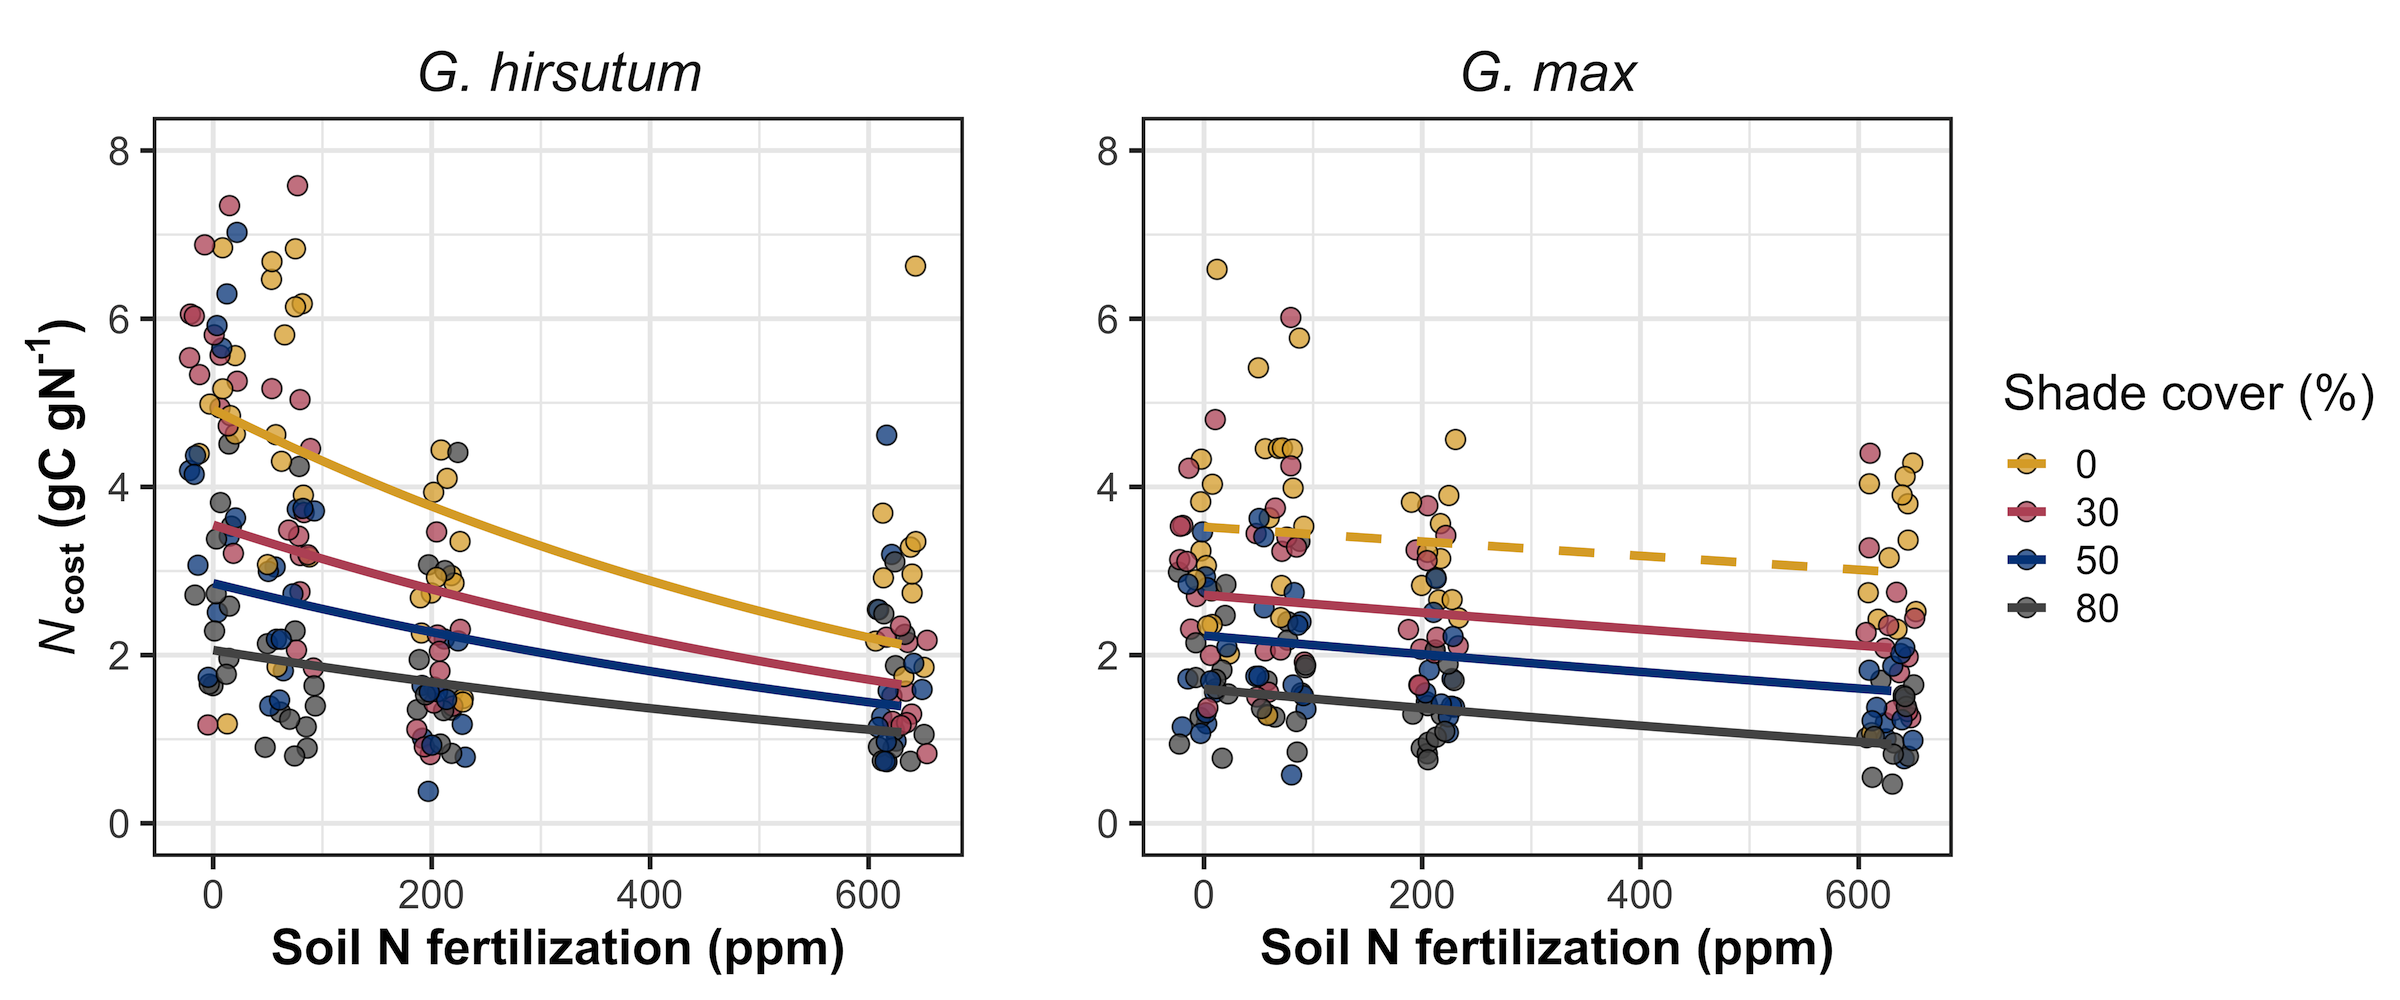
\includegraphics[width=\textwidth]{ch2_LxN_Greenhouse/figs/fig1_ncost.png}
    \centering
    \caption[Relationships between soil nitrogen fertilization and light availability on carbon costs to acquire nitrogen in \textit{G. hirsutum} and \textit{G. max}]{Relationships between soil nutrient fertilization and light availability on carbon costs to acquire nitrogen in \textit{G. hirsutum} and \textit{G. max}. Nitrogen fertilization treatments are represented on the x-axis. Shade cover treatments are represented through colored points and trendlines. Trendlines were created by back-transforming marginal mean slopes and intercepts from species-specific linear mixed-effects models. These values were calculated using the ‘emtrends’ and ‘emmeans’ functions in the ‘emmeans’ R package (Lenth, 2019). Points are jittered for visibility. Yellow points and trendlines represent the 0\% shade cover treatment, blue points and trendlines represent the 30\% shade cover treatment, green points and trendlines represent the 50\% shade cover treatment, and purple points and trendlines represent the 80\% shade cover treatment. Solid trendlines indicate slopes that are significantly different from zero (Tukey: \textit{p} < 0.05), while dashed trendlines indicate slopes that are not statistically different from zero.}

    \label{fig:figure2.1}
\end{figure}
\clearpage


\newpage
\subsection{\textit{Whole plant nitrogen biomass}}
Whole-plant nitrogen biomass in \textit{G. hirsutum} was driven by an interaction between light availability and nitrogen fertilization (\textit{p} = 0.001; Table \ref{tab:table2.1}; Fig. \ref{fig:figure2.2}). This interaction indicated a greater stimulation of whole-plant nitrogen biomass by nitrogen fertilization as light levels increased (Table \ref{tab:table2.1}; Fig. \ref{fig:figure2.2}).

Whole-plant nitrogen biomass in \textit{G. max} increased with increasing light availability (\textit{p} < 0.001) and nitrogen fertilization (\textit{p} < 0.001), with no interaction between light availability and nitrogen fertilization (\textit{p} = 0.231; Table \ref{tab:table2.1}; Fig. \ref{fig:figure2.2}).

\newpage
\begin{figure}
    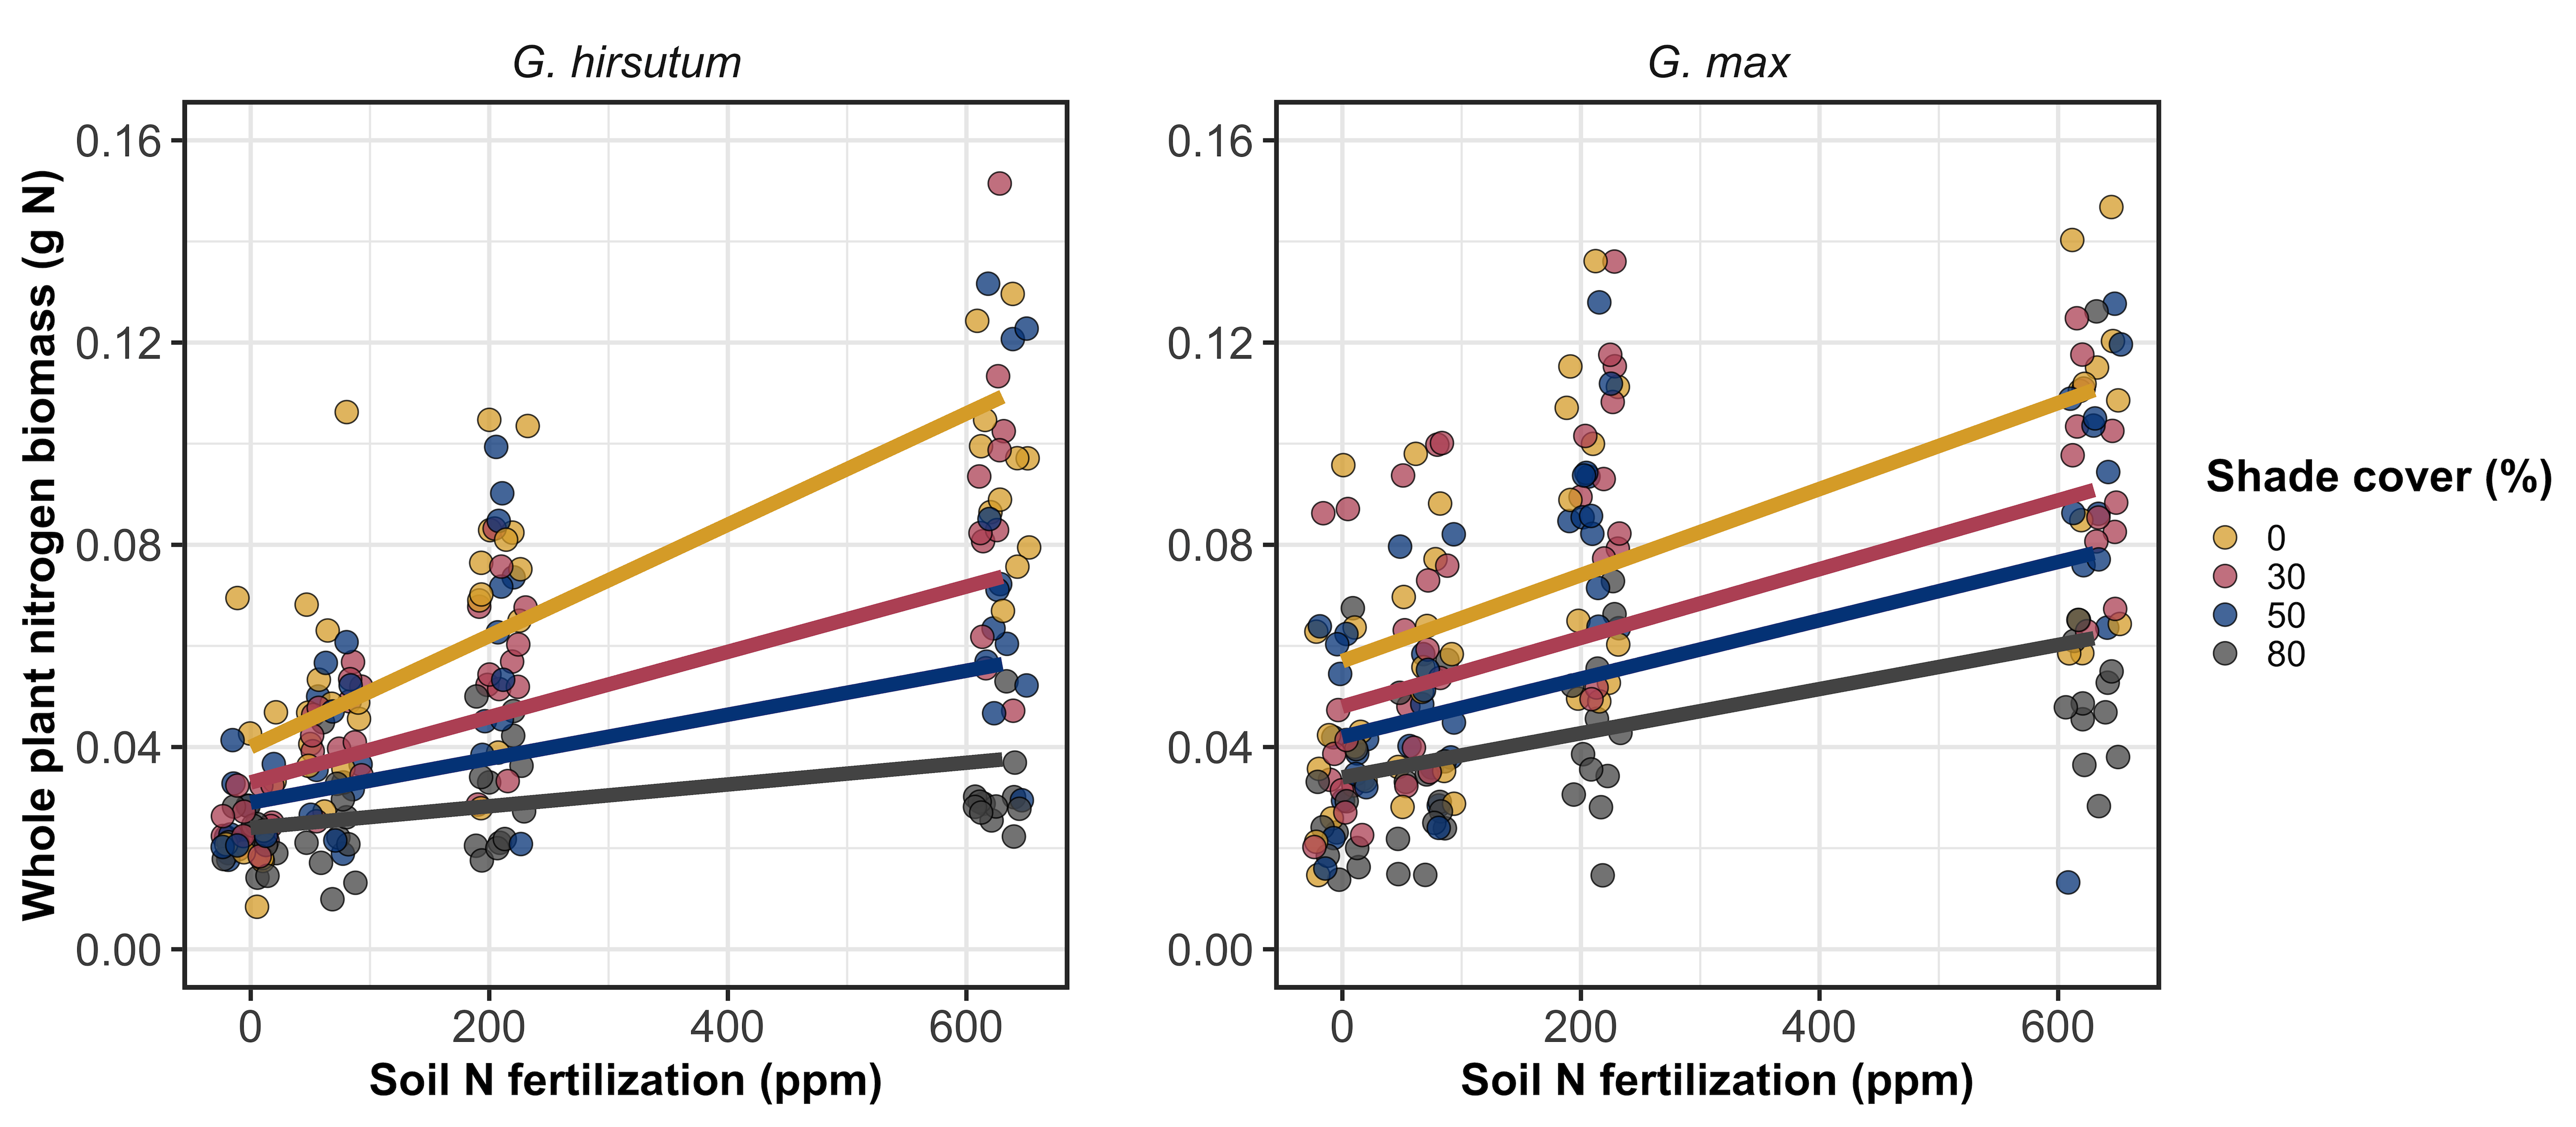
\includegraphics[width=\textwidth]{ch2_LxN_Greenhouse/figs/fig2_nacq.png}
    \centering
    \caption[Relationships between soil nitrogen fertilization and light availability on whole-plant nitrogen biomass in \textit{G. hirsutum} and \textit{G. max}]{Relationships between soil nutrient fertilization and light availability on whole-plant nitrogen biomass in \textit{G. hirsutum} and \textit{G. max}.Whole-plant nitrogen biomass is the denominator of the carbon cost to acquire nitrogen calculation. Nitrogen fertilization treatments are represented on the x-axis. Shade cover treatments are represented through colored points and trendlines. Trendlines were created by back-transforming marginal mean slopes and intercepts from species-specific linear mixed-effects models. These values were calculated using the ‘emtrends’ and ‘emmeans’ functions in the ‘emmeans’ R package \shortcite{Lenth2019}. Points are jittered for visibility. Yellow points and trendlines represent the 0\% shade cover treatment, blue points and trendlines represent the 30\% shade cover treatment, green points and trendlines represent the 50\% shade cover treatment, and purple points and trendlines represent the 80\% shade cover treatment. Solid trendlines indicate slopes that are significantly different from zero (Tukey: P<0.05), while dashed trendlines indicate slopes that are not statistically different from zero.}
    \label{fig:figure2.2}
    \small
\end{figure}
\clearpage

\newpage
\subsection{\textit{Root carbon biomass}}
Root carbon biomass in \textit{G. hirsutum} significantly increased with increasing light availability (\textit{p} < 0.001; Table \ref{tab:table2.1}; Fig. \ref{fig:figure2.3}) and marginally increased with nitrogen fertilization (\textit{p} = 0.089; Table \ref{tab:table2.1}; Fig. \ref{fig:figure2.3}). There was also a marginal interaction between light availability and nitrogen fertilization (\textit{p} = 0.076; Table \ref{tab:table2.1}), driven by an increase in the positive response of root carbon biomass to increasing nitrogen fertilization as light availability increased. This resulted in significantly positive trends between root carbon biomass and nitrogen fertilization in the two highest light treatments (Tukey: \textit{p} < 0.05 in both cases; Table \ref{tab:table2.3}; Fig. \ref{fig:figure2.3}) and no effect of nitrogen fertilization in the two lowest light treatments (Tukey: \textit{p} > 0.05 in both cases; Table \ref{tab:table2.3}; Fig. \ref{fig:figure2.3}). 

There was an interaction between light availability and nitrogen fertilization on root carbon biomass in \textit{G. max} (\textit{p} = 0.001; Table \ref{tab:table2.1}; Fig. \ref{fig:figure2.3}). Post-hoc analyses indicated that the positive effects of nitrogen fertilization on \textit{G. max} root carbon biomass increased with increasing light availability (Table \ref{tab:table2.3}; Fig. \ref{fig:figure2.3}). There were also positive individual effects of increasing nitrogen fertilization (\textit{p} < 0.001) and light availability (\textit{p} < 0.001) on \textit{G. max} root carbon biomass (Table \ref{tab:table2.1}; Fig. \ref{fig:figure2.3}).

\newpage
\begin{figure}
    \centering
    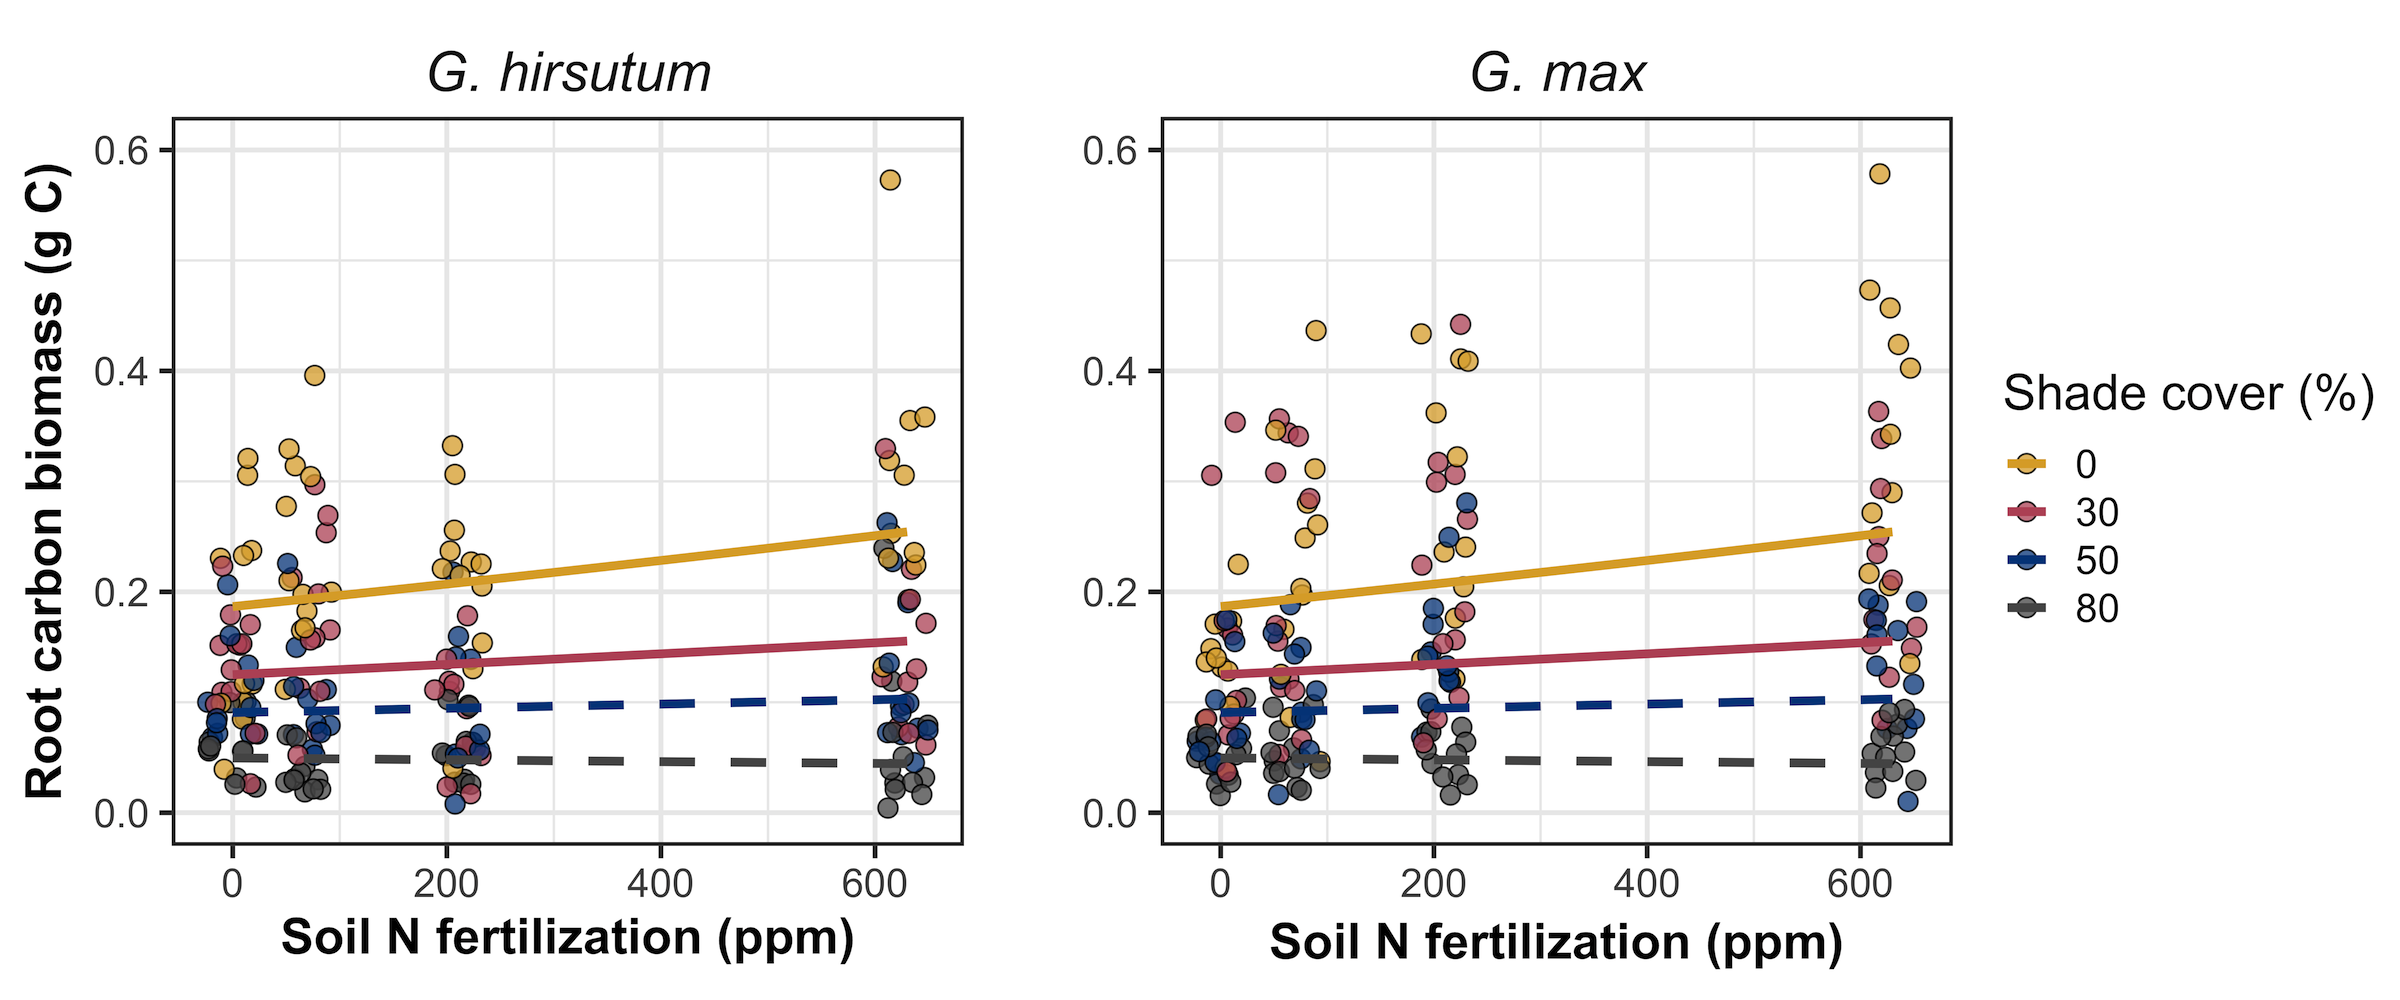
\includegraphics[width=\textwidth]{ch2_LxN_Greenhouse/figs/fig3_rootCarbon.png}
    \caption[Relationships between soil nitrogen fertilization and light availability on root carbon biomass in \textit{G. hirsutum} and \textit{G. max}]{Relationships between soil nutrient fertilization and light availability on root carbon biomass in \textit{G. hirsutum} and \textit{G. max}. Root carbon biomass is the numerator of the carbon cost to acquire nitrogen calculation. Nitrogen fertilization treatments are represented on the x-axis. Shade cover treatments are represented through colored points and trendlines. Trendlines were created by back-transforming marginal mean slopes and intercepts from species-specific linear mixed-effects models. These values were calculated using the ‘emtrends’ and ‘emmeans’ functions in the ‘emmeans’ R package \shortcite{Lenth2019}. Points are jittered for visibility. Yellow points and trendlines represent the 0\% shade cover treatment, blue points and trendlines represent the 30\% shade cover treatment, green points and trendlines represent the 50\% shade cover treatment, and purple points and trendlines represent the 80\% shade cover treatment. Solid trendlines indicate slopes that are significantly different from zero (Tukey: \textit{p} < 0.05), while dashed trendlines indicate slopes that are not statistically different from zero.}
    \label{fig:figure2.3}
\end{figure}
\clearpage

\newpage
\subsection{\textit{Root nodule biomass}}
Root nodule biomass in \textit{G. max} increased with increasing light availability (\textit{p} < 0.001; Table \ref{tab:table2.2}; Fig. \ref{fig:figure2.4}A) and decreased with increasing nitrogen fertilization (\textit{p} < 0.001; Table \ref{tab:table2.2}; Fig. \ref{fig:figure2.4}A). There was no interaction between nitrogen fertilization and light availability (\textit{p} = 0.133; Table \ref{tab:table2.2}; Fig. \ref{fig:figure2.4}A). The ratio of root nodule biomass to root biomass did not change in response to light availability (\textit{p} = 0.481; Table \ref{tab:table2.2}; Fig. \ref{fig:figure2.4}B) but decreased with increasing nitrogen fertilization (\textit{p} < 0.001; Table \ref{tab:table2.2}; Fig. \ref{fig:figure2.4}B). There was no interaction between nitrogen fertilization and light availability on the ratio of root nodule biomass to root biomass (\textit{p} = 0.621; Table \ref{tab:table2.2}; Fig. \ref{fig:figure2.4}B).

\newpage
\begin{table}[]
    \caption{Analysis of variance results exploring effects of light availability, nitrogen fertilization, and their interactions on \textit{G. max} root nodule biomass and the ratio of root nodule biomass to root biomass\textsuperscript{$*$}}
    \centering
    \resizebox{\columnwidth}{!}{
    \begin{tabular}{p{2.5cm}p{0.5cm}p{2cm}p{1.5cm}p{1.5cm}p{2cm}p{1.5cm}p{1.5cm}}
        && 
        \multicolumn{3}{l}{Nodule biomass} & \multicolumn{3}{l}{Nodule biomass: root biomass} 
        \\
        \hline
        & \multicolumn{1}{r}{df}
        & \multicolumn{1}{r}{Coefficient}   & \multicolumn{1}{r}{$\chi^{2}$}        & \multicolumn{1}{r}{\textit{p}}
        & \multicolumn{1}{r}{coefficient}   & \multicolumn{1}{r}{$\chi^{2}$}        & \multicolumn{1}{r}{\textit{p}}
        \\
        \hline
        
        (Intercept)
        && \multicolumn{1}{r}{0.302}        & \multicolumn{1}{r}{-}                 & \multicolumn{1}{r}{-}
        & \multicolumn{1}{r}{0.448}         & \multicolumn{1}{r}{-}                 & \multicolumn{1}{r}{-} 
        \\
    
        Light (L) & \multicolumn{1}{r}{1}
        & \multicolumn{1}{r}{-1.81E-03}     & \multicolumn{1}{r}{72.964}            & \multicolumn{1}{r}{\textbf{\textless{}0.001}}
        & \multicolumn{1}{r}{-8.76E-05}     & \multicolumn{1}{r}{0.496}             & \multicolumn{1}{r}{0.481} 
        \\
    
        Nitrogen (N) & \multicolumn{1}{r}{1}
        & \multicolumn{1}{r}{-2.83E-04}     & \multicolumn{1}{r}{115.377}           & \multicolumn{1}{r}{\textbf{\textless{}0.001}}
        & \multicolumn{1}{r}{-5.09E-04}     & \multicolumn{1}{r}{156.476}           & \multicolumn{1}{r}{\textbf{\textless{}0.001}} 
        \\
    
        L*N & \multicolumn{1}{r}{1}
        &  \multicolumn{1}{r}{1.14E-06}     &   \multicolumn{1}{r}{2.226}           & \multicolumn{1}{r}{0.133}
        & \multicolumn{1}{r}{-7.30E-07}     &   \multicolumn{1}{r}{0.244}           & \multicolumn{1}{r}{0.621}
        \\
        \hline
        \\
        
        \multicolumn{8}{p{16cm}}{*Significance determined using Wald’s $\chi^{2}$ tests ($\alpha$ = 0.05). \textit{p}-values less than 0.05 are in bold. Negative coefficients for light treatments indicate a positive effect of increasing light availability on all response variables, as light availability is treated as percent shade cover in all linear mixed-effects models. Root nodule biomass and nodule biomass: root biomass models were only constructed for \textit{G. max} because \textit{G. hirsutum} was not inoculated with \textit{B. japonicum} and is not capable of forming root nodules.}
    \end{tabular}}
    \label{tab:table2.2}
\end{table}
\clearpage

\newpage
\begin{landscape}
    \begin{table}[]
        \caption{Slopes of the regression line describing the relationship between each dependent variable and nitrogen fertilization at each light level\textsuperscript{$\ast$}} 
        \centering
        \resizebox{\columnwidth}{!}{
            \begin{tabular}{p{2cm}p{3cm}p{3cm}p{3cm}p{3cm}p{3cm}}
             \hline
              \begin{tabular}[c]{@{}l@{}}Shade \\ cover\end{tabular}
              & \begin{tabular}[c]{@{}l@{}}Carbon cost to \\ acquire nitrogen\end{tabular}
              & \begin{tabular}[c]{@{}l@{}}Whole-plant \\ nitrogen biomass\end{tabular}
              & \begin{tabular}[c]{@{}l@{}}Root carbon \\ biomass\end{tabular}
              & \begin{tabular}[c]{@{}l@{}}Root nodule\\ biomass\end{tabular}
              & \begin{tabular}[c]{@{}l@{}}Nodule biomass\:\\ root biomass\end{tabular} \\
              \hline
              \multicolumn{1}{l}{\textit{G. hirsutum}} \\
              \multicolumn{1}{r}{0\%}
              &  \multicolumn{1}{r}{\textbf{-1.34E-03\textsuperscript{a}}}
              &  \multicolumn{1}{r}{\textbf{ 1.83E-03\textsuperscript{a}}}
              &  \multicolumn{1}{r}{\textbf{ 1.15E-04\textsuperscript{b}}}
              &  \multicolumn{1}{r}{-}
              &  \multicolumn{1}{r}{-}
              \\
              \multicolumn{1}{r}{30\%}                     
              &  \multicolumn{1}{r}{\textbf{-1.22E-03\textsuperscript{a}}}
              &  \multicolumn{1}{r}{\textbf{ 1.43E-03\textsuperscript{a}}}
              &  \multicolumn{1}{r}{\textbf{ 1.17E-04\textsuperscript{b}}}
              &  \multicolumn{1}{r}{-}
              &  \multicolumn{1}{r}{-}
               \\
              \multicolumn{1}{r}{50\%}
              &  \multicolumn{1}{r}{\textbf{-1.14E-03\textsuperscript{a}}}
              &  \multicolumn{1}{r}{\textbf{ 1.17E-03\textsuperscript{a}}}
              &           \multicolumn{1}{r}{3.12E-05\textsuperscript{b}}
              & \multicolumn{1}{r}{-}
              & \multicolumn{1}{r}{-}
              \\
              \multicolumn{1}{r}{80\%}
              &  \multicolumn{1}{r}{\textbf{-1.02E-03\textsuperscript{a}}}
              &  \multicolumn{1}{r}{\textbf{ 7.66E-04\textsuperscript{a}}}
              &  \multicolumn{1}{r}{-1.89E-06\textsuperscript{b}}
              &   \multicolumn{1}{r}{-}
              &   \multicolumn{1}{r}{-}
              \\
              &&&& 
              \\
              \multicolumn{1}{l}{\textit{G. max}}
              \\
              \multicolumn{1}{r}{0\%}
              &  \multicolumn{1}{r}{ -2.35E-04\textsuperscript{b}}
              &  \multicolumn{1}{r}{\textbf{ 1.55E-05\textsuperscript{b}}}
              &  \multicolumn{1}{r}{\textbf{ 2.51E-04\textsuperscript{b}}}
              &  \multicolumn{1}{r}{\textbf{-2.83E-04\textsuperscript{b}}}
              &  \multicolumn{1}{r}{\textbf{-5.09E-04\textsuperscript{b}}}
              \\
              
              \multicolumn{1}{r}{30\%}
              &  \multicolumn{1}{r}{\textbf{-3.22E-04\textsuperscript{b}}}
              &  \multicolumn{1}{r}{\textbf{ 1.35E-05\textsuperscript{b}}}
              &  \multicolumn{1}{r}{\textbf{ 1.57E-04\textsuperscript{b}}}
              &  \multicolumn{1}{r}{\textbf{-2.49E-04\textsuperscript{b}}}
              &  \multicolumn{1}{r}{\textbf{-5.31E-04\textsuperscript{b}}}
              \\
              
              \multicolumn{1}{r}{50\%}
              &  \multicolumn{1}{r}{\textbf{-3.80E-04\textsuperscript{b}}}
              &  \multicolumn{1}{r}{\textbf{ 1.23E-05\textsuperscript{b}}}
              &  \multicolumn{1}{r}{\textbf{ 9.37E-05\textsuperscript{b}}}
              &  \multicolumn{1}{r}{\textbf{-2.26E-04\textsuperscript{b}}}
              &  \multicolumn{1}{r}{\textbf{-5.45E-04\textsuperscript{b}}}
              \\
              
              \multicolumn{1}{r}{80\%}
              &  \multicolumn{1}{r}{\textbf{-4.66E-04\textsuperscript{b}}}
              &  \multicolumn{1}{r}{\textbf{ 1.04E-05\textsuperscript{b}}}
              &  \multicolumn{1}{r}{-9.95E-07\textsuperscript{b}}
              &  \multicolumn{1}{r}{\textbf{-1.92E-04\textsuperscript{b}}}
              &  \multicolumn{1}{r}{\textbf{-5.67E-04\textsuperscript{b}}}  
              \\
              \hline
              \multicolumn{6}{p{20cm}}{*Slopes represent estimated marginal mean slopes from linear mixed-effects models described in the Methods. Slopes were calculated using the ‘emmeans’ R package \shortcite{Lenth2019}. Superscripts indicate slopes fit to natural-log (\textsuperscript{a}) or square root (\textsuperscript{b}) transformed data. Slopes statistically different from zero (Tukey: \textit{p} < 0.05) are indicated in bold. Marginally significant slopes (Tukey: 0.05 < \textit{p} < 0.1) are italicized.}
            \end{tabular}}
            \label{tab:table2.3}
        \end{table}
    \end{landscape}
    \clearpage

\newpage
\begin{figure}
    \centering
    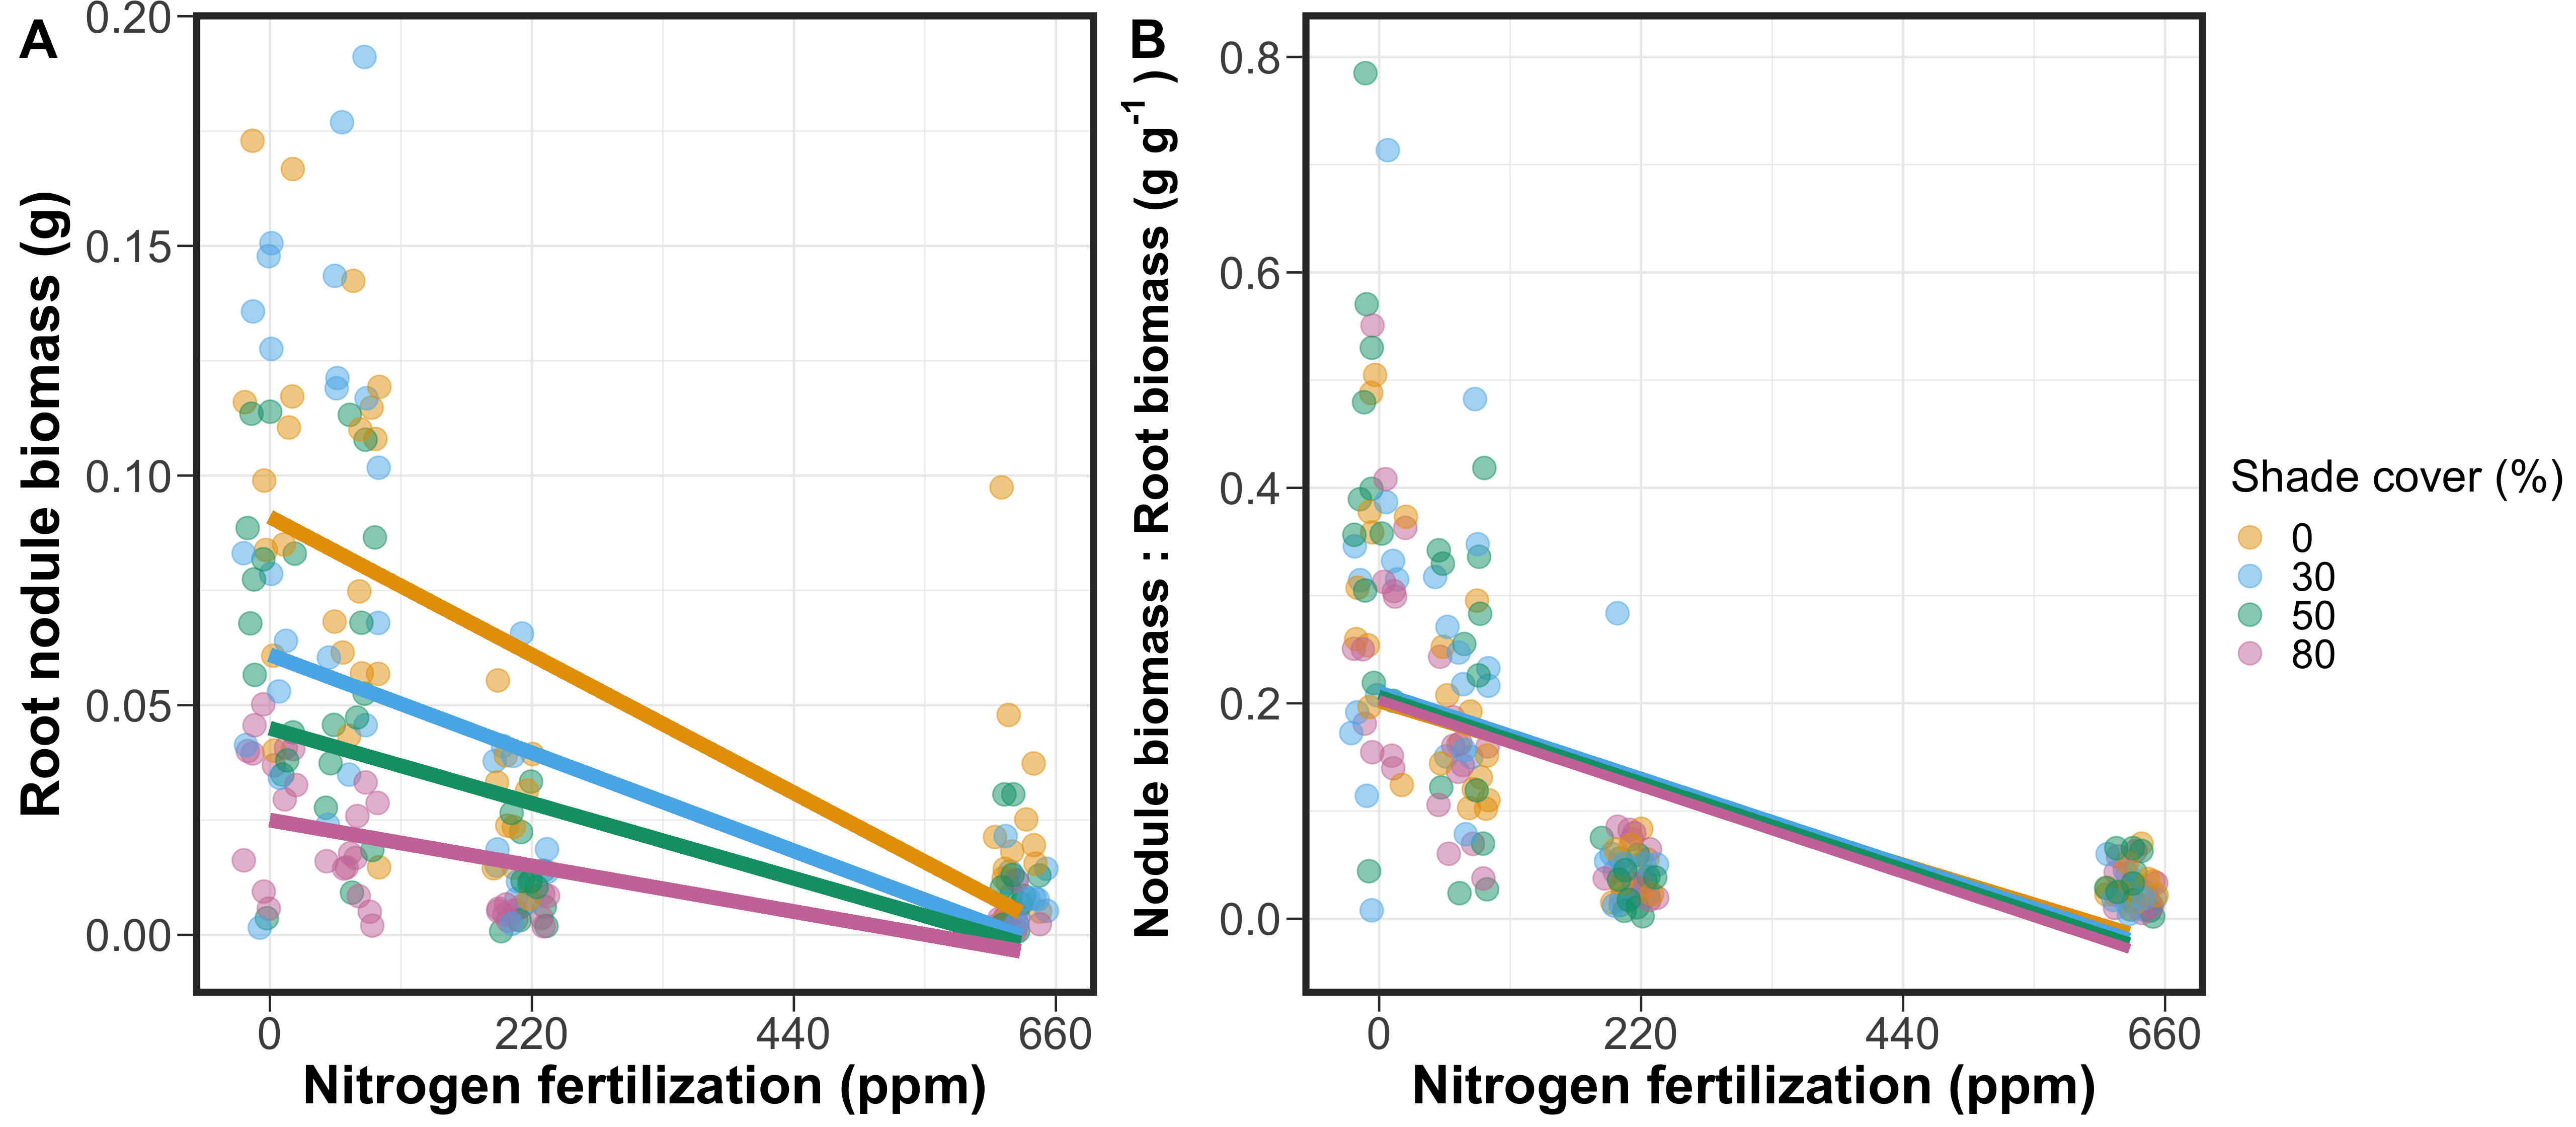
\includegraphics[width=\textwidth]{ch2_LxN_Greenhouse/figs/fig4_nodwgt.png}
    \caption[Effects of shade cover and nitrogen fertilization on root nodule biomass and the ratio of root nodule biomass to root biomass in \textit{G. max}.]{Effects of shade cover and nitrogen fertilization on root nodule biomass (A) and the ratio of root nodule biomass to root biomass (B) in \textit{G. max}. Nitrogen fertilization treatments are represented on the x-axis. Shade cover treatments are represented through colored points and trendlines. Trendlines were created by back-transforming marginal mean slopes and intercepts from species-specific linear mixed-effects models. These values were calculated using the ‘emtrends’ and ‘emmeans’ functions in the ‘emmeans’ R package \shortcite{Lenth2019}. Points are jittered for visibility. Yellow points and trendlines represent the 0\% shade cover treatment, blue points and trendlines represent the 30\% shade cover treatment, green points and trendlines represent the 50\% shade cover treatment, and purple points and trendlines represent the 80\% shade cover treatment. Solid trendlines indicate slopes that are significantly different from zero (Tukey: \textit{p} < 0.05), while dashed trendlines indicate slopes that are not statistically different from zero.}
    \label{fig:figure2.4}
\end{figure}
\clearpage

\section{Discussion}
In this chapter, we determined the effects of light availability and soil nitrogen fertilization on root mass carbon costs to acquire nitrogen in \textit{G. hirsutum} and \textit{G. max}. In support of our hypotheses, we found that carbon costs to acquire nitrogen generally increased with increasing light availability and decreased with increasing soil nitrogen fertilization in both species. These findings suggest that carbon costs to acquire nitrogen are determined by factors that influence plant nitrogen demand and soil nitrogen availability. In contrast to our second hypothesis, root nodulation data suggested that \textit{G. max} and \textit{G. hirsutum} achieved similar directional carbon cost responses to nitrogen fertilization despite a likely shift in G.!max allocation from nodulation to root biomass along the nitrogen fertilization gradient (Fig. \ref{fig:figure2.4}B).

Both \textit{G. max} and \textit{G. hirsutum} experienced an increase in carbon costs to acquire nitrogen due to increasing light availability. These patterns were driven by a larger increase in root carbon biomass than whole-plant nitrogen biomass. Increases in root carbon biomass due to factors that increase plant nitrogen demand are a commonly observed pattern, as carbon allocated belowground provides substrate needed to produce and maintain structures that satisfy aboveground plant nitrogen demand \shortcite{Nadelhoffer1992,Giardina2005,Raich2014}. Our findings suggest that plants allocate relatively more carbon for acquiring nitrogen when demand increases over short temporal scales, which may cause a temporary state of diminishing return due to asynchrony between belowground carbon and whole-plant nitrogen responses to plant nitrogen demand \shortcite{Kulmatiski2017,Noyce2019}. These responses might be attributed to a temporal lag associated with producing structures that enhance nitrogen acquisition. For example, fine roots \shortcite{Matamala2000,Norby2004,Arndal2018} and root nodules \shortcite{Parvin2020} take time to build and first require the construction of coarse roots. Thus, full nitrogen returns from these investments may not occur immediately \shortcite{Kayler2010,Kayler2017}, and may vary by species acquisition strategy. We speculate that increases in nitrogen acquisition from a given carbon investment may occur beyond the 5 week scope of this experiment. A similar study conducted over a longer temporal scale would address this.

Increasing soil nitrogen fertilization generally decreased carbon costs to acquire nitrogen in both species. These patterns were driven by a larger increase in whole-plant nitrogen biomass than root carbon biomass. In \textit{G. hirsutum}, reductions in carbon costs to acquire nitrogen may have been due to an increase in per-root nitrogen uptake, allowing individuals to maximize the amount of nitrogen acquired from a belowground carbon investment. Interestingly, increased soil nitrogen fertilization increased whole-plant nitrogen biomass in \textit{G. max} despite reductions in root nodule biomass that likely reduced the nitrogen-fixing capacity of \textit{G. max} \shortcite{Andersen2005,Munoz2016}. While reductions in root nodulation due to increased soil nitrogen availability are commonly observed \shortcite{Gibson1985,Fujikake2003}, our responses were observed in tandem with increased root carbon biomass, implying that \textit{G. max} shifted relative carbon allocation from nitrogen fixation to soil nitrogen acquisition \shortcite{Markham2007,Dovrat2020}. This was likely because there was a reduction in the carbon cost advantage of acquiring fixed nitrogen relative to soil nitrogen, and suggests that species capable of associating with symbiotic nitrogen-fixing bacteria shift their relative nitrogen acquisition pathway to optimize nitrogen uptake \shortcite{Rastetter2001}. Future studies should further investigate these patterns with a larger quantity of phylogenetically related species, or different varieties of a single species that differ in their ability to form associations with symbiotic nitrogen-fixing bacteria to more directly test the impact of nitrogen fixation on the patterns observed in this study.

Carbon costs to acquire nitrogen are subsumed in the general discussion of economic analogies to plant resource uptake \shortcite{Bloom1985,Rastetter2001,Vitousek2002,Phillips2013,Terrer2018,Henneron2020}. Despite this, terrestrial biosphere models rarely include these carbon costs within their framework for predicting plant nitrogen uptake. There is currently one plant resource uptake model, FUN, that quantitatively predicts carbon costs to acquire nitrogen within a framework for predicting plant nitrogen uptake for different nitrogen acquisition strategies \shortcite{Fisher2010,Brzostek2014FUN2}

\shortcite{Fisher2010,Brzostek2014FUN2}. Iterations of FUN are currently coupled to two terrestrial biosphere models: the Community Land Model 5.0 and the Joint UK Land Environment Simulator \shortcite{Shi2016,Lawrence2019,Clark2011}. Recent work suggests that coupling FUN to CLM 5.0 caused a large overprediction of plant nitrogen uptake associated with nitrogen fixation \shortcite{Davies-Barnard2020}. Thus, empirical data from manipulative experiments that explicitly quantify carbon costs to acquire nitrogen in species capable of associating with nitrogen-fixing bacteria across different environmental contexts is an important step toward identifying potential biases in models such as FUN.

Our findings broadly support the FUN formulation of carbon costs to acquire nitrogen in response to soil nitrogen availability. FUN calculates carbon costs to acquire nitrogen based on the sum of carbon costs to acquire nitrogen via nitrogen fixation, mycorrhizal active uptake, non-mycorrhizal active uptake, and retranslocation \shortcite{Fisher2010,Brzostek2014FUN2}. Carbon costs to acquire nitrogen via mycorrhizal or non-mycorrhizal active uptake pathways are derived as a function of nitrogen availability, root biomass, and two parameterized values based on nitrogen acquisition strategy \shortcite{Brzostek2014FUN2}. Due to this, FUN simulates a net decrease in carbon costs to acquire nitrogen with increasing nitrogen availability for mycorrhizal and non-mycorrhizal active uptake pathways, assuming constant root biomass. This was a pattern we observed in \textit{G. hirsutum} regardless of light availability. In contrast, FUN would not simulate a net change in carbon costs to acquire nitrogen via nitrogen fixation due to nitrogen availability. This is because carbon costs to acquire nitrogen via nitrogen fixation are derived from a well-established function of soil temperature, which is independent of soil nitrogen availability \shortcite{Houlton2008,Fisher2010}. We observed a net reduction in carbon costs to acquire nitrogen in \textit{G. max}, except when individuals were grown under 0\% shade cover (Fig. \ref{fig:figure2.1}). While a net reduction of carbon costs in response to nitrogen fertilization runs counter to nitrogen fixation carbon costs simulated by FUN, these patterns were likely because \textit{G. max} individuals switched their primary mode of nitrogen acquisition from symbiotic nitrogen fixation to a non-symbiotic active uptake pathway (Fig. \ref{fig:figure2.4}B).

It should be noted that the metric used in this study to determine carbon costs to acquire nitrogen has several limitations. Most notably, this metric uses root carbon biomass as a proxy for estimating the amount of carbon spent on nitrogen acquisition. While it is true that most carbon allocated belowground has at least an indirect structural role in acquiring soil resources, it remains unclear whether this assumption holds true for species that acquire nitrogen via symbiotic nitrogen fixation. We also cannot quantify carbon lost through root exudates or root turnover, which may increase due to factors that increase plant nitrogen demand \shortcite{Tingey2000,Phillips2011}, and can increase the magnitude of available nitrogen from soil organic matter through priming effects on soil microbial communities \shortcite{Uselman2000,Bengtson2012}. It is also not clear whether these assumptions hold under all environmental conditions, such as those that shift belowground carbon allocation toward a different mode of nitrogen acquisition \shortcite{Taylor2018,Friel2019} or between species with different acquisition strategies. In this study, increasing soil nitrogen fertilization increased carbon investment to roots relative to carbon transferred to root nodules (Fig. \ref{fig:figure2.4}B). By assuming that carbon allocated to root carbon was proportional to carbon allocated to root nodules across all treatment combinations, these observed responses to soil nitrogen fertilization were likely to be overestimated in \textit{G. max}. We encourage future research to quantify these carbon fates independently.

Researchers conducting pot experiments must carefully choose pot volume to minimize the likelihood of pot volume-induced growth limitation \shortcite{Poorter2012}. \shortciteN{Poorter2012} indicate that researchers are likely to avoid growth limitations associated with pot volume if measurements are collected when the plant biomass:pot volume ratio is less than 1 g L\textsuperscript{-1}. In this experiment, all treatment combinations in both species had biomass:pot volume ratios less than 1 g L\textsuperscript{-1} except for \textit{G. max} and \textit{G. hirsutum} that were grown under 0\% shade cover and had received 630 ppm N. Specifically, \textit{G. max} and \textit{G. hirsutum} had average respective biomass:pot volume ratios of 1.24$\pm$0.07 g L\textsuperscript{-1} and 1.34$\pm$0.13 g L\textsuperscript{-1}, when grown under 0\% shade cover and received 630 ppm N (Supplementary Tables S2, S3; Supplementary Fig. S1). If growth in this treatment combination was limited by pot volume, then individuals may have had larger carbon costs to acquire nitrogen than would be expected if they were grown in larger pots. This pot volume induced growth limitation could cause a reduction in per-root nitrogen uptake associated with more densely packed roots, which could reduce the positive effect of nitrogen fertilization on whole-plant nitrogen biomass relative to root carbon biomass \shortcite{Poorter2012}.

Growth limitation associated with pot volume provides a possible explanation for the marginally insignificant effect of increasing nitrogen fertilization on \textit{G. max} carbon costs to acquire nitrogen when grown under 0\% shade cover (Table \ref{tab:table2.3}; Fig. \ref{fig:figure2.1}). This is because the regression line describing the relationship between carbon costs to acquire nitrogen and nitrogen fertilization in \textit{G. max} grown under 0\% shade cover would have flattened if growth limitation had caused larger than expected carbon costs to acquire nitrogen in the 0\% shade cover, 630 ppm N treatment combination. This may have been exacerbated by the fact that \textit{G. max} likely shifted relative carbon allocation from nitrogen fixation to soil nitrogen acquisition, which could have increased the negative effect of more densely packed roots on nitrogen uptake. These patterns could have also occurred in \textit{G. hirsutum} grown under 0\% shade cover; however, there was no change in the effect of nitrogen fertilization on \textit{G. hirsutum} carbon costs to acquire nitrogen grown under 0\% shade cover relative to other shade cover treatments. Regardless, the possibility of growth limitation due to pot volume suggests that effects of increasing nitrogen fertilization on carbon costs to acquire nitrogen in both species grown under 0\% shade cover could have been underestimated. Follow-up studies using a similar experimental design with a larger pot volume would be necessary in order to determine whether these patterns were impacted by pot volume-induced growth limitation.

In conclusion, this study provides empirical evidence that carbon costs to acquire nitrogen are influenced by light availability and soil nitrogen fertilization in a species capable of acquiring nitrogen via symbiotic nitrogen fixation and a species not capable of forming such associations. We show that carbon costs to acquire nitrogen generally increase with increasing light availability and decrease with increasing nitrogen fertilization. This study provides important empirical data needed to evaluate the formulation of carbon costs to acquire nitrogen in terrestrial biosphere models, particularly carbon costs to acquire nitrogen that are associated with symbiotic nitrogen fixation. Our findings broadly support the general formulation of these carbon costs in the FUN biogeochemical model in response to shifts in nitrogen availability. However, there is a need for future studies to explicitly quantify carbon costs to acquire nitrogen under different environmental contexts, over longer temporal scales, and using larger selections of phylogenetically related species. In addition, we suggest that future studies minimize the limitations associated with the metric used here by explicitly measuring belowground carbon fates independently.


%%%%%%%%%%%%%%%%%%%%%%%%%%%%%%%%%%%%%%%%%%%%%%%%
%End LxN greenhouse experiment chapter           %
%%%%%%%%%%%%%%%%%%%%%%%%%%%%%%%%%%%%%%%%%%%%%%%%

%%%%%%%%%%%%%%%%%%%%%%%%%%%%%%%%%%%%%%%%%%%%%%%%%%
%%%%%%%%%%%%%%%%%%%%%%%%%%%%%%%%%%%%%%%%%%%%%%%%%%
%%%%%%%%%%%%%%%%%%%%%%%%%%%%%%%%%%%%%%%%%%%%%%%%%%
%Start NxS field experiment chapter              %
%%%%%%%%%%%%%%%%%%%%%%%%%%%%%%%%%%%%%%%%%%%%%%%%%%
%%%%%%%%%%%%%%%%%%%%%%%%%%%%%%%%%%%%%%%%%%%%%%%%%%
%%%%%%%%%%%%%%%%%%%%%%%%%%%%%%%%%%%%%%%%%%%%%%%%%%
\begin{singlespace}
    \chapter{\textbf{Soil nitrogen availability modifies leaf nitrogen economies in mature temperate deciduous forests: a direct test of photosynthetic least-cost theory}}
\end{singlespace}
    
\section{Introduction}
\noindent Photosynthesis represents the largest carbon flux between the atmosphere and land surface \shortcite{IPCC2021}, and plays a central role in biogeochemical cycling at multiple spatial and temporal scales \shortcite{Vitousek1991,LeBauer2008,Kaiser2015,Wieder2015_NPP}. Therefore, carbon and energy fluxes simulated by terrestrial biosphere models are sensitive to the formulation of photosynthetic processes \shortcite{Ziehn2011,Bonan2011,Booth2012,Smith2016,Smith2017} and must be represented using robust, empirically tested processes \shortcite{Prentice2015,Wieder2019}. Current formulations of photosynthesis vary across terrestrial biosphere models \shortcite{Smith2013,Rogers2017a}, which causes variation in modeled ecosystem processes \shortcite{Knorr2000,KnorrHeimann2001,Bonan2011,Friedlingstein2014} and casts uncertainty on the ability of these models to accurately predict terrestrial ecosystem responses and feedbacks to global change \shortcite{Zaehle2005,Schaefer2012,Davies-Barnard2020}.

Terrestrial biosphere models commonly represent C$_{3}$ photosynthesis th-rough variants of the \shortciteN{Farquhar1980} biochemical model \shortcite{Smith2013,Rogers2014,Rogers2017a}. This well-tested photosynthesis model estimates leaf-level carbon assimilation, or photosynthetic capacity, as a function of the maximum rate of Ribulose-1,5-bisphosphate carboxylase-oxygenase (Ru-bisco) carboxylation ($V_\mathrm{cmax}$) and the maximum rate of Ribulose-1,5-bisphosphate (RuBP) regeneration ($J_\mathrm{max}$) \shortcite{Farquhar1980}. Many terrestrial biosphere models predict these model inputs based on plant functional group specific linear relationships between leaf nutrient content and $V_\mathrm{cmax}$ \shortcite{Smith2013,Rogers2014,Rogers2017a} under the tenet that a large fraction of leaf nutrients, and nitrogen in particular, are partitioned toward building and maintaining enzymes that support photosynthetic capacity, such as Rubisco \shortcite{Brix1971,Gulmon1981,Evans1989_photoN,Kattge2009,Walker2014}. Terrestrial biosphere models predict leaf nutrient content from soil nutrient availability based on the assumption that increasing soil nutrients generally increases leaf nutrients \shortcite{Firn2019,Li2020,Liang2020} which, in the case of nitrogen, generally corresponds with an increase in photosynthetic processes \shortcite{Li2020,Liang2020}.

Recent work calls the generality of relationships between soil nutrient availability, leaf nutrient content, and photosynthetic capacity into question, suggesting instead that leaf nutrients and photosynthetic capacity are better predicted as an integrated product of aboveground climate, leaf traits, and soil nutrient availability, rather than soil nutrient availability alone \shortcite{Dong2017,Dong2020,Dong2022a,Firn2019,Smith2019,Peng2021}. It has been reasoned that this result is because plants allocate added nutrients to growth and storage rather than alterations in leaf chemistry \shortcite{Smith2019}, perhaps as a result of nutrient limitation of primary productivity \shortcite{LeBauer2008,Fay2015}. Additionally, recent work suggests that relationships between leaf nutrient content and photosynthesis vary across environments, and that the proportion of leaf nutrient content allocated to photosynthetic tissue varies over space and time with plant acclimation and adaptation responses to light availability, vapor pressure deficit, soil pH, soil nutrient availability, and environmental factors that influence leaf mass per area \shortcite{Pons1994,Niinemets1997,Evans2001,Hikosaka2009,Ghimire2017,Onoda2017,Luo2021}. The use of linear relationships between leaf nutrient content and $V_\mathrm{cmax}$ to predict photosynthetic capacity, as commonly used in terrestrial biosphere models \shortcite{Rogers2014}, is not capable of detecting such responses.

Photosynthetic least-cost theory provides an alternative framework for understanding relationships between soil nutrient availability, leaf nutrient content, and photosynthetic capacity \shortcite{Harrison2021}. Leveraging a two-input microeconomics approach \shortcite{Wright2003}, the theory posits that plants acclimate to a given environment by optimizing leaf photosynthesis rates at the lowest summed cost of using nutrients and water \shortcite{Prentice2014,Wang2017,Smith2019,Paillassa2020}. Across resource availability gradients, the theory predicts that optimal photosynthetic rates can be achieved by trading less efficient use of a resource that is less costly to acquire (or more abundant) for more efficient use of a resource more costly to acquire (or less abundant). For example, an increase in soil nutrient availability should reduce the cost of acquiring and using nutrients \shortcite{Bae2015,Eastman2021,Perkowski2021}, which could increase leaf nutrient investments in photosynthetic proteins to allow similar photosynthetic rates to be achieved with higher nutrient use (lower nutrient use efficiency) but lower water use (greater water use efficiency). The theory suggests similar tradeoffs in response to increasing soil pH \shortcite{Paillassa2020}, specifically, that increasing soil pH should reduce the cost of acquiring soil nutrients due to an increase in plant-available nutrient concentration \shortcite{Paillassa2020,Dong2022a}. The theory is also capable of reconciling dynamic leaf nutrient-photosynthesis relationships at global scales \shortcite{Luo2021}.

Patterns expected from photosynthetic least-cost theory have recently received empirical support both in global environmental gradient \shortcite{Smith2019,Paillassa2020,Luo2021,Querejeta2022,Westerband2023} and local manipulative invasion \shortcite{BialicMurphy2021} studies. However, nutrient addition experiments that directly examine nutrient-water use tradeoffs expected from the theory are rare (but see Guerrieri et al. 2011), and only global gradient studies testing the theory have considered soil pH in their analyses. As a result, there is a need to use nutrient addition and soil pH manipulation experiments to test mechanisms driving responses predicted by the theory.

In this study, I measured leaf responses to soil nitrogen availability in five deciduous tree species growing in the upper canopy of mature closed canopy temperate forests in the northeastern United States. Soil nitrogen availability and pH were manipulated through a nitrogen-by-pH field manipulation experiment with treatments applied since 2011, eight years prior to measurement. Two different soil nitrogen treatments were applied to increase nitrogen availability with opposing effects on soil pH. An additional nitrogen-free acidifying treatment was expected to decrease soil pH. I hypothesized that increased soil nitrogen availability would enable plants to increase nutrient uptake and create more photosynthetic enzymes per leaf, allowing similar photosynthetic rates achieved with lower leaf C$_\mathrm{i}$:C$_\mathrm{a}$ and increased leaf nitrogen content allocated to photosynthetic leaf tissue. I expected that this response would be driven by a reduction in the cost of acquiring nitrogen, which would cause trees to sacrifice efficient nitrogen use to enable more efficient use of other limiting resources (i.e., water). Finally, I hypothesized similar leaf responses to increasing soil pH.

\section{Methods}
\subsection{\textit{Study site description}}
\noindent I conducted this study in summer 2019 at three stands located within a 20-km radius of Ithaca, NY, USA (42.444 \textdegree{}N, 76.502 \textdegree{}W). All stands contain mature, closed-canopy forests dominated by deciduous tree species. Stands contained abundant sugar maple (\textit{Acer saccharum} Marshall), American beech (\textit{Fagus grandifolia} Ehrh.), and white ash (\textit{Fraxinus americana} L.), accounting for 43\%, 15\%, and 17\% of the total aboveground biomass across the three stands, respectively, with less frequent red maple (\textit{Acer rubrum} L.; 9\% of total aboveground biomass) and red oak occurrences (\textit{Quercus rubra} L.; 10\% of total aboveground biomass). Soils at each site were broadly classified as a channery silt loam Inceptisols using the USDA NRCS Web Soil Survey data product \shortcite{SoilSurveyStaff2022}. Between 2006 and 2020, study sites averaged 972 mm of precipitation per year and had an average temperature of 7.9 \textdegree{}C per a weather station located near the Cornell University campus (42.449 \textdegree{}N, 76.449 \textdegree{}W) part of the NOAA NCEI Global Historical Climatology Network \shortcite{Menne2012}.

\subsection{\textit{Experimental design}}
\noindent Four 40 m x 40 m plots were set up at each site in 2009, each with an additional 10 m buffer along plot perimeters (60 m x 60 m total). The plots were set up as a nitrogen-by-pH field manipulation experiment, with one each of four treatments at each site. Two nitrogen treatments were applied, both at 50 $\mathrm{kg\ N\ ha^{-1}\ yr^{-1}}$, as either sodium nitrate ($\mathrm{NaNO_3}$) to raise soil pH, or ammonium sulfate $\mathrm{((NH_4)_{2}SO_4)}$ to acidify; an elemental sulfur treatment was selected to acidify without nitrogen, applied at the same rate of S addition (57 $\mathrm{kg\ S\ ha^{-1}\ yr^{-1}}$); and control plots received no additions. All amendments were added in pelletized form using hand-held fertilizer spreaders to both the main plots and buffers. Amendments were divided into three equal doses distributed across the growing season from 2011-2017 and added as a single dose from 2018 onward. During 2019, plots were fertilized during the week of May 20.

\subsection{\textit{Leaf gas exchange and trait measurements}}
\noindent I sampled one leaf each from 6 to 10 individuals per plot between June 25 and July 12, 2019 for gas exchange measurements (Table \ref{table:tab.b1}). Leaves were collected from deciduous broadleaf trees represented across all sites and plots and were replicated in efforts to mimic the species abundance of each plot at each site. I attempted to collect leaves from the upper canopy to reduce differential shading effects on leaf physiology. Leaves were accessed by pulling down small branches using an arborist’s slingshot and weighted beanbag attached to a throw line. Branches were immediately recut under deionized water and remained submerged to reduce stomatal closure and avoid xylem embolism, as done in \shortciteN{Smith2018}, until gas exchange data were collected.

Randomly selected leaves with little to no visible external damage were attached to a Li-COR LI-6800 (Li-COR Bioscience, Lincoln, Nebraska, USA) portable photosynthesis machine to measure net photosynthesis ($A_\mathrm{net}$; $\mathrm{\mu mol\ m^{-2}}$ $\mathrm{{s}^{-1}}$), stomatal conductance ($g_\mathrm{sw}$; $\mathrm{mol\ m^{-2}\ s^{-1}}$), and intercellular CO$_2$ concentration ($C_\mathrm{i}$; $\mathrm{\mu mol\ mol^{-1}}$) at different reference CO$_2$ concentrations ($C_\mathrm{a}$; $\mathrm{\mu mol\ mol^{-1}}$) concentrations (i.e., an $A_\mathrm{net}/C_\mathrm{i}$ curve) under saturating light conditions (2,000 $\mathrm{\mu mol\ m^{-2}\ s^{-1}}$). Reference CO$_2$ concentrations followed the sequence: 400, 300, 200, 100, 50, 400, 400, 600, 800, 1000, 1200, 1500, and 2000 $\mathrm{\mu mol\ mol^{-1}\ CO_2}$. Leaf temperatures were not controlled in the cuvette and ranged from 21.8 \textdegree{}C to 31.7 \textdegree{}C (mean$\pm$SD: 27.2$\pm$2.2 \textdegree{}C). A linear and second order log-polynomial nonlinear regression suggested no effect of temperature on stomatal conductance measured at 400 $\mathrm{\mu mol\ mol^{-1}\ CO_2}$ or net photosynthesis measured at 400 $\mathrm{\mu mol\ mol^{-1}\ CO_2}$ (Table \ref{table:tab.b2}, \ref{table:tab.b3}; Fig. \ref{fig:figure.b1}). All $A_\mathrm{net}$/$C_\mathrm{i}$ curves were generated within one hour of branch severance.

Leaf morphological and chemical traits were collected on the same leaf used to generate each $A_\mathrm{net}/C_\mathrm{i}$ curve. Images of each leaf were taken using a flat-bed scanner to determine fresh leaf area using the ‘LeafArea’ R package \shortcite{Katabuchi2015}, which automates leaf area calculations using ImageJ software \shortcite{Schneider2012}. Each leaf was dried at 65\textdegree{}C for at least 48 hours, weighed, and ground using a Retsch MM200 ball mill grinder (Verder Scientific, Inc., Newtown, PA, USA) until homogenized. Leaf mass per unit leaf area ($M_\mathrm{area}$, g m$^{-2}$) was calculated as the ratio of dry leaf biomass to fresh leaf area. Using a subsample of ground and homogenized leaf biomass, leaf nitrogen content ($N_\mathrm{mass}$; gN g$^{-1}$) and leaf $\mathrm{\delta^{13}C}$ (‰, relative to Vienna Pee Dee Belemnite international reference standard) were measured at the Cornell Stable Isotope Lab with an elemental analyzer (NC 2500, CE Instruments, Wigan, UK) interfaced to an isotope ratio mass spectrometer (Delta V Isotope Ratio Mass Spectrometer, ThermoFisher Scientific, Waltham, MA, USA). Leaf nitrogen content per unit leaf area ($N_\mathrm{area}$; gN m$^{-2}$) was calculated by multiplying $N_\mathrm{mass}$ by $M_\mathrm{area}$.

I used leaf $\mathrm{\delta^{13}}$C values to estimate $\chi$ (unitless), which is an isotope-derived estimate of the leaf $C_\mathrm{i}$:$C_\mathrm{a}$ ratio. While intercellular and atmospheric CO$_2$ concentrations were directly measured during each $A_\mathrm{net}$/$C_\mathrm{i}$ curve, deriving $\chi$ from $\mathrm{\delta^{13}}$C provides a more integrative estimate of the leaf $C_\mathrm{i}$:$C_\mathrm{a}$ over an individual leaf’s lifespan. I derived $\chi$ following the approach of \shortciteN{Farquhar1989} described in \shortciteN{Cernusak2013}:

\begin{equation} \label{eq_2.1}
    \chi= \frac{\Delta^{13}C-a}{b-a}
\end{equation}

\noindent where $\mathrm{\Delta^{13}}$C represents the relative difference between leaf $\mathrm{\delta^{13}}$C (‰) and air $\mathrm{\delta^{13}}$C (‰), and is calculated from the following equation:

\begin{equation} \label{eq_2.2}
    \Delta^{13}C= \frac{\delta^{13}C_{air}-\delta^{13}C_{leaf}}{1+\delta^{13}C_{leaf}}
\end{equation}
    
\noindent where $\mathrm{\delta^{13}C_{air}}$ is assumed to be -8‰ \shortcite{Keeling1979,Farquhar1989}, \textit{a} represents the fractionation between $^{12}$C and $^{13}$C due to diffusion in air, assumed to be 4.4‰, and \textit{b} represents the fractionation caused by Rubisco carboxylation, assumed to be 27‰ \shortcite{Farquhar1989}.
    
\subsection{$A_{net}/C_i$ \textit{curve-fitting and parameter estimation}}
\noindent I fit $A_\mathrm{net}/C_\mathrm{i}$ curves of each individual using the ‘fitaci’ function in the ‘plantecophys’ R package \shortcite{Duursma2015}. This function estimates the maximum rate of Rubisco carboxylation ($V_\mathrm{cmax}$; $\mathrm{\mu mol\ m^{-2}\ s^{-1}}$) and maximum rate of electron transport for RuBP regeneration ($J_\mathrm{max}$; $\mathrm{\mu mol\ m^{-2}\ s^{-1}}$) based on the Farquhar, von Caemmerer, and Berry biochemical model of C$_{3}$ photosynthesis \shortcite{Farquhar1980}. For each curve fit, I included triose phosphate utilization (TPU) limitation to avoid underestimating $J_{\mathrm{max}}$ \shortcite{Gregory2021}. Curves were visually examined to confirm the likely presence of TPU limitation. 
    
I determined Michaelis-Menten coefficients for Rubisco affinity to CO$_2$ ($K_\mathrm{c}$; $\mathrm{\mu mol\ mol^{-1}}$) and $\mathrm{O_2}$ ($K_\mathrm{o}$; $\mathrm{\mu mol\ mol^{-1}}$), and the CO$_2$ compensation point ($\Gamma^*$; $\mathrm{\mu mol\ mol^{-1}}$) using leaf temperature and equations described in \shortciteN{Medlyn2002} and derived in \shortciteN{Bernacchi2001}. Specifically, $K_\mathrm{c}$ and $K_\mathrm{o}$ were calculated as:

\begin{equation} \label{eq_2.3}
    K_\mathrm{c}=404.9*exp^{\frac{79430(T_\mathrm{k}-298)}{298RT_\mathrm{k}}}
\end{equation}
    
\noindent and
    
\begin{equation} \label{eq_2.4}
    K_\mathrm{o}=278.4*exp^{\frac{36380(T_\mathrm{k}-298)}{298RT_\mathrm{k}}}
\end{equation}
    
\noindent while $\Gamma^*$ was calculated as:
    
\begin{equation} \label{eq_2.5}
    \Gamma^\mathrm{*}=42.75*exp^{\frac{37830(T_\mathrm{k}-298)}{298RT_\mathrm{k}}}
\end{equation}

\noindent In all three equations, $T_\mathrm{k}$ is the leaf temperature (in Kelvin) during each $A_\mathrm{net}/C_\mathrm{i}$ curve and R is the universal gas constant (8.314 J mol$^{-1}$ K$^{-1}$).

I standardized $V_\mathrm{cmax}$ and $J_\mathrm{max}$ estimates to 25 \textdegree{}C using a modified Arrhenius equation \shortcite{Kattge2007}:

\begin{equation} \label{eq_2.6}
    k_\mathrm{25}=\frac{k_\mathrm{obs}}{e^{\frac{H_a(T_{obs}-T_{ref})}{T_{ref}RT_{obs}}}*\frac{1+e^{\frac{T_{ref}\Delta S-H_d}{T_{ref}}}}{1+e^{\frac{T_{obs}\Delta S-H_d}{T_{obs}}}}}
\end{equation}

\noindent $k_\mathrm{25}$ represents the standardized $V_\mathrm{cmax}$ or $J_\mathrm{max}$ rate at 25\textdegree{}C, $k_\mathrm{obs}$ represents the $V_\mathrm{cmax}$ or $J_\mathrm{max}$ estimate at the average leaf temperature measured inside the cuvette during the $A_\mathrm{net}$/$C_\mathrm{i}$ curve. $H_\mathrm{a}$ is the activation energy of $V_{\mathrm{cmax}}$ (71,513 J mol$^{-1}$) \shortciteN{Kattge2007} or $J_\mathrm{max}$ (49,884 J mol$^{-1}$) \shortcite{Kattge2007}. $H_\mathrm{d}$ represents the deactivation energy of both $V_\mathrm{cmax}$ and $J_\mathrm{max}$ (200,000 J mol$^{-1}$) \shortcite{Medlyn2002}, and R represents the universal gas constant (8.314 J mol$^{-1}$ K$^{-1}$). $T_\mathrm{ref}$ represents the standardized temperature of 298.15 K (25\textdegree{}C) and $T_\mathrm{obs}$ represents the mean leaf temperature (in K) during each $A_\mathrm{net}$/$C_\mathrm{i}$ curve. $\Delta$S is an entropy term that \shortcite{Kattge2007} derived as a linear relationship with average growing season temperature ($T_\mathrm{g}$; \textdegree{}C), where: 

\begin{equation} \label{eq_2.7}
    \Delta S_{vcmax}=-1.07\ T_{g}+668.39
\end{equation}
    
\noindent and
   
\begin{equation} \label{eq_2.8}
    \Delta S_{jmax}=-0.75\ T_{g}+659.70
\end{equation}

\noindent I estimated $T_\mathrm{g}$ in Equations \ref{eq_2.7} and \ref{eq_2.8} based on mean daily (24-hour) air temperature of the 30 days leading up to the day of each sample collection using the same weather station reported in the site description. I used $V_\mathrm{cmax25}$ and $J_\mathrm{max25}$ estimates to calculate the ratio of $J_\mathrm{max25}$ to $V_\mathrm{cmax25}$ ($J_\mathrm{max25}$:$V_\mathrm{cmax25}$; unitless).

\subsection{\textit{Proportion of leaf nitrogen allocated to photosynthesis and structure}}
\noindent I used equations from \shortciteN{Niinemets1997} to estimate the proportion of leaf nitrogen content allocated to Rubisco and bioenergetics. The proportion of leaf nitrogen allocated to Rubisco ($\rho_\mathrm{rubisco}$; gN gN$^{-1}$) was calculated as a function of $V_\mathrm{cmax25}$ and $N_\mathrm{area}$: 

\begin{equation} \label{eqn_2.9}
    \rho_{rubisco}=\frac{V_{cmax25}N_r}{V_{cr}N_{area}}
\end{equation}

\noindent where $N_\mathrm{r}$ is the amount of nitrogen in Rubisco, set to 0.16 $\mathrm{gN\ (gN\ in\ Rubisco)^{-1}}$ and $V_\mathrm{cr}$ is the maximum rate of RuBP carboxylation per unit Rubisco protein, set to 20.5 $\mathrm{\mu mol\ CO_2\ (g\ Rubisco)^{-1}}$. The proportion of leaf nitrogen allocated to bioenergetics ($\mathrm{\rho_{bioe}}$; gN gN$^{-1}$) was similarly calculated as a function of $J_\mathrm{max25}$ and $N_\mathrm{area}$:

\begin{equation} \label{eqn_2.10}
    \rho_{bioe}=\frac{J_{max25}N_b}{J_{mc}N_{area}}
\end{equation}

\noindent where $N_\mathrm{b}$ is the amount of nitrogen in cytochrome f, set to 0.12407 gN ($\mu\mathrm{mol}$ cytochrome f)$^{-1}$ assuming a constant 1: 1: 1.2 cytochrome f: ferredoxin NADP reductase: coupling factor molar ratio \shortcite{EvansSeemann1989,Niinemets1997}, and $J_\mathrm{mc}$ is the capacity of electron transport per cytochrome f, set to 156 $\mathrm{\mu mol\ electron\ (\mu mol\ cytochrome\ f)^{-1} s^{-1}}$.

I estimated the proportion of leaf nitrogen content allocated to photosynthetic tissue ($\rho_\mathrm{photo}$; gN gN$^{-1}$) as the sum of $\rho_\mathrm{rubisco}$ and $\rho_\mathrm{bioe}$. This calculation is an underestimate of the proportion of leaf nitrogen allocated to photosynthetic tissue because it does not include nitrogen allocated to light harvesting proteins. This leaf nitrogen pool was not included because I did not perform chlorophyll extractions on focal leaves. However, the proportion of leaf nitrogen content allocated to light harvesting proteins tends to be small relative to $\rho_\mathrm{rubisco}$ and $\rho_\mathrm{bioe}$, and may scale with changes in $\rho_\mathrm{rubisco}$ and $\rho_\mathrm{bioe}$ \shortcite{Niinemets1997}.

Finally, the proportion of leaf nitrogen content allocated to structural tissue ($\rho_\mathrm{structure}$; gN gN$^{-1}$) was estimated as:
\begin{equation} \label{eqn_3.11}
    \rho_{structure}=\frac{N_{cw}}{N_{area}}
\end{equation}
\noindent where $N_\mathrm{cw}$ is the leaf nitrogen content allocated to cell walls (gN m$^{-2}$), calculated as a function of $M_\mathrm{area}$ using an empirical equation from \shortciteN{Onoda2017}:
\begin{equation} \label{eqn_3.12}
    N_{cw}=0.000355*{M_{area}}^{1.39}
\end{equation}


\subsection{\textit{Tradeoffs between nitrogen and water use}}
\noindent Photosynthetic nitrogen use efficiency (PNUE; $\mathrm{\mu mol\ CO_2\ mol^{-1}\ N\ s^{-1}}$) was calculated by dividing $A_\mathrm{net}$ by $N_\mathrm{area}$, first converting $N_\mathrm{area}$ to $\mathrm{mol\ N\ m^{-2}}$ using the molar mass of nitrogen (14 $\mathrm{g\ mol^{-1}}$). I used $\chi$ as an indicator of water use efficiency, which exploratory analyses suggest had similar responses to soil nitrogen availability and pH as intrinsic water use efficiency measured from gas exchange ($A_\mathrm{net}$/$g_\mathrm{sw}$). Tradeoffs between nitrogen and water use were determined by calculating the ratio of $N_\mathrm{area}$ to $\chi$ ($N_\mathrm{area}$:$\chi$; gN m$^{-2}$) and $V_\mathrm{cmax25}$ to $\chi$ ($V_\mathrm{cmax25}$:$\chi$; $\mathrm{\mu mol\ m^{-2}\ s^{-1}}$). This approach is similar to tradeoff calculations in which nitrogen-water use tradeoffs are measured as the ratio of $N_\mathrm{area}$ or $V_\mathrm{cmax25}$ to $g_\mathrm{sw}$ \shortcite{Paillassa2020,BialicMurphy2021}. In this chapter, I quantify these relationships using $\chi$ in lieu of $g_\mathrm{sw}$ because $g_\mathrm{sw}$ rapidly changes with environmental conditions and therefore may have been altered by recent tree branch severance and/or placement in the cuvette.

\subsection{\textit{Soil nitrogen availability and pH}}
\noindent To characterize soil nitrogen availability at the time of our leaf gas exchange measurements, I used mixed bed resin bags to quantify mobile ammonium-N and nitrate-N concentrations in each plot. Lycra mesh bags were filled with 5 g of Dowex\textregistered\ Marathon MR-3 hydrogen and hydroxide form resin (MilliporeSigma, Burlington, MA USA) and sealed with a zip tie. Each bag was activated by soaking in 0.5 M HCl for 20 minutes, then in 2 M NaCl until pH of the saline solution stabilized, as described in \shortciteN{Allison2008a}. Five resin bags were inserted about 10 cm below the soil surface at each plot on June 25, 2019: one near each of the four plot corners and one near the plot center. All resin bags were collected 24 days later on July 19, 2019 and were frozen until extracted.
    
Prior to anion and cation extraction, each resin bag was rinsed with ultrapure water (MilliQ IQ 7000; Millipore Sigma, Burlington, MA) to remove any surface soil residues. Anions and cations were extracted from surface-cleaned resin bags by individually soaking and shaking each bag in 100 mL of a 0.1 M HCl/2.0 M NaCl matrix for one hour. Using a microplate reader (Biotek Synergy H1; Biotek Instruments, Winooski, VT USA), I quantified nitrate-N concentrations spectrophotometrically at 540 nm with the end product of a single reagent vanadium (III) chloride reaction \shortcite{Doane2003}, and ammonium-N concentrations quantified at 650 nm with the end product of a modified phenol-hypochlorite reaction \shortcite{Weatherburn1967,Rhine1998}. Both the single reagent vanadium (III) chloride and modified phenol-hypochlorite methodologies are well established for determining nitrate-N and ammonium-N concentrations in resin bag extracts \shortcite{Arnone1997,Allison2008a}. I used a series of negative and positive controls throughout each well plate to verify the accuracy and precision of our measurements, assaying each resin bag extract and control in triplicate. Soil nitrogen availability was estimated as the sum of the nitrate-N and ammonium-N concentration in each resin bag, normalized per g of resin and duration in the field ($\mathrm{\mu g\ N\ g^{-1}\ resin\ d^{-1}}$), then subsequently averaged across all resin bags in a plot for a plot-level mean.
    
Soil pH was measured on 0-10 cm mineral soil samples collected prior to fertilization in 2019. Near each of the four plot corners, three 5.5 cm diameter soil cores were collected after first removing the forest floor where present. Each set of three cores was placed in a plastic bag, and later composited by hand mixing and sieved to 4mm. Soil pH was determined for a 1:2 soil:water slurry (10 g field-moist soil to 20 mL DI water) of each sample using an Accumet AB15 pH meter with flushable junction probe (Fisher Scientific; Hampton, NH, USA), and was estimated at the plot level as the mean soil pH within each plot.

\subsection{\textit{Statistical analyses}}
\noindent I built two separate series of linear mixed-effects models to explore effects of soil nitrogen availability, soil pH, species, and leaf nitrogen content on leaf physiological traits. In the first series of linear mixed-effects models, I explored the effect of soil nitrogen availability, soil pH, and species on leaf nitrogen content, leaf photosynthesis, stomatal conductance, and nitrogen-water use tradeoffs. Models included plot-level soil nitrogen availability and plot-level soil pH as continuous fixed effects, species as a categorical fixed effect, and site as a categorical random intercept term. Interaction terms between fixed effects were not included due to the small number of experimental plots. I built a series of separate models with this independent variable structure to quantify individual effects of soil nitrogen availability, soil pH, and species on $N_\mathrm{area}$, $M_\mathrm{area}$, $N_\mathrm{mass}$, $A_\mathrm{net}$, $V_\mathrm{cmax25}$, $J_\mathrm{max25}$, $J_\mathrm{max25}$:$V_\mathrm{cmax25}$, $\rho_\mathrm{rubisco}$, $\rho_\mathrm{bioenergetics}$, $\rho_\mathrm{photo}$, $\rho_\mathrm{structure}$, $\chi$, PNUE, $N_\mathrm{area}$:$\chi$, and $V_\mathrm{cmax25}$:$\chi$.

A second series of linear mixed-effects models were built to investigate relationships between leaf nitrogen content and photosynthetic parameters. Statistical models included $N_\mathrm{area}$ as a single continuous fixed effect with species and site designated as individual random intercept terms. I used this independent variable structure to quantify individual effects of leaf nitrogen content on $A_\mathrm{net}$, $V_\mathrm{cmax25}$, $J_\mathrm{max25}$, $J_\mathrm{max25}$:$V_\mathrm{cmax25}$, and $\chi$.

For all linear mixed-effects models, I used Shapiro-Wilk tests of normality to determine whether linear mixed-effects models satisfied residual normality assumptions. If residual normality assumptions were not met, then models were fit using dependent variables that were natural log transformed. If residual normality assumptions were still not met (Shapiro-Wilk: \textit{p}<0.05), then models were fit using dependent variables that were square root transformed. All residual normality assumptions for both sets of models that did not originally satisfy residual normality assumptions were met with either a natural log or square root data transformation (Shapiro-Wilk: \textit{p}>0.05 in all cases).

In the first series of models, models for $N_\mathrm{area}$, $M_\mathrm{area}$, $N_\mathrm{mass}$, $V_\mathrm{cmax25}$, $J_\mathrm{max25}$, $\chi$, $N_{\mathrm{area}}$:$\chi$, and $V_\mathrm{cmax25}$:$\chi$, $\rho_\mathrm{rubisco}$, $\rho_\mathrm{bioenergetics}$, $\rho_\mathrm{photo}$, $\rho_\mathrm{structure}$ satisfied residual normality assumptions without data transformations (Shapiro-Wilk: \textit{p}>0.05 in all cases). The model for $J_\mathrm{max25}$:$V_\mathrm{cmax25}$ satisfied residual normality assumptions with a natural log data transformation, while models for $A_\mathrm{net}$ and PNUE each satisfied residual normality assumptions with square root data transformations. In the second series of models, models for $V_\mathrm{cmax25}$, $J_\mathrm{max25}$, $\chi$, and $V_\mathrm{cmax25}$:$\chi$ satisfied residual normality assumptions without data transformations (Shapiro-Wilk: \textit{p}>0.05 in all cases). The model for $J_\mathrm{max25}$:$V_\mathrm{cmax25}$ required a natural log data transformation and the model for $A_\mathrm{net}$ required a square root data transformation (Shapiro-Wilk: \textit{p}>0.05 in both cases).
    
In all models, I used the ‘lmer’ function in the ‘lme4’ R package \shortcite{Bates2015} to fit each model and the ‘Anova’ function in the ‘car’ R package \shortcite{Fox2019} to calculate Type II Wald’s $\chi^2$ and determine the significance level ($\alpha$=0.05) of each fixed effect coefficient. Finally, I used the ‘emmeans’ R package (Lenth, 2019) to conduct post-hoc comparisons using Tukey’s tests, where degrees of freedom were approximated using the Kenward-Roger approach \shortcite{Kenward1997}. All analyses and plots were conducted in R version 4.1.1 \shortcite{RCoreTeam2021}. All figure regression lines and associated 95\% confidence interval error bars were plotted using predictions generated across the soil nitrogen availability gradient using the ‘emmeans’ R package \shortcite{Lenth2019}.
    
\section{Results}
\subsection{\textit{Leaf nitrogen content}}  
\noindent Increasing soil nitrogen availability generally increased $N_\mathrm{area}$ (Table \ref{tab:table3.1}; Fig. \ref{fig:figure3.1}a). This pattern was driven by an increase in $N_\mathrm{mass}$ (Table \ref{tab:table3.1}; Fig. \ref{fig:figure3.1}c) and a marginal increase in $M_\mathrm{area}$ (Table \ref{tab:table3.1}; Fig. \ref{fig:figure3.1}e) with increasing soil nitrogen availability. There was no effect of soil pH on $N_\mathrm{area}$, $N_\mathrm{mass}$, or $M_\mathrm{area}$ (Table \ref{tab:table3.1}); however, I also observed strong differences in $N_\mathrm{area}$ (Fig. \ref{fig:figure3.1}b), $N_\mathrm{mass}$ (Fig. \ref{fig:figure3.1}d), and $M_\mathrm{area}$ (Fig. \ref{fig:figure3.1}e) between species (Table \ref{tab:table3.1}).
    \clearpage

    \newpage
    \begin{landscape}
        \begin{table}[]
        \centering
        \caption[Effects of soil nitrogen availability, soil pH, and species on leaf nitrogen content per unit leaf area, leaf nitrogen content per unit leaf mass, and leaf mass per unit leaf area]{Effects of soil nitrogen availability, soil pH, and species on leaf nitrogen content per unit leaf area ($N_\mathrm{area}$; gN m$^{-2}$), leaf nitrogen content per unit leaf mass ($N_\mathrm{mass}$; gN g$^{-1}$), and leaf mass per unit leaf area ($M_\mathrm{area}$; g m$^{-2}$)$^*$}
        \resizebox{\columnwidth}{!}{
        \begin{tabular}{p{2.5cm}p{0.5cm}p{2cm}p{1.5cm}p{1.5cm}p{2cm}p{1.5cm}p{1.5cm}p{2cm}p{1.5cm}p{1.5cm}}
                 && 
                 \multicolumn{3}{l}{$N_\mathrm{area}$} 
                 & \multicolumn{3}{l}{$N_\mathrm{mass}$} 
                 & \multicolumn{3}{l}{$M_\mathrm{area}$} 
                 \\
                 \hline 
                 & 
                 \multicolumn{1}{r}{df} 
                 & \multicolumn{1}{r}{Coefficient} & \multicolumn{1}{r}{$\chi^{2}$} & \multicolumn{1}{r}{\textit{p}} 
                 & \multicolumn{1}{r}{Coefficient} & \multicolumn{1}{r}{$\chi^{2}$} & \multicolumn{1}{r}{\textit{p}} 
                 & \multicolumn{1}{r}{Coefficient} & \multicolumn{1}{r}{$\chi^{2}$} & \multicolumn{1}{r}{\textit{p}} 
                 \\ 
                 \hline

                 Intercept & \multicolumn{1}{r}{-} 
                 &  \multicolumn{1}{r}{9.03E$-$01} & \multicolumn{1}{r}{-} & \multicolumn{1}{r}{-}
                 &  \multicolumn{1}{r}{1.68E+00} & \multicolumn{1}{r}{-} & \multicolumn{1}{r}{-}
                 &  \multicolumn{1}{r}{4.60E+01} & \multicolumn{1}{r}{-} & \multicolumn{1}{r}{-} 
                 \\

                 Soil N & \multicolumn{1}{r}{1}
                 & \multicolumn{1}{r}{1.68E$-$02} & \multicolumn{1}{r}{11.990} & \multicolumn{1}{r}{\textbf{0.001}}
                 & \multicolumn{1}{r}{1.25E$-$02}  & \multicolumn{1}{r}{6.902} & \multicolumn{1}{r}{\textbf{0.009}}
                 & \multicolumn{1}{r}{4.87E$-$01}  & \multicolumn{1}{r}{4.143} & \multicolumn{1}{r}{\textbf{0.042}} 
                 \\


                 Soil pH & \multicolumn{1}{r}{1}
                 & \multicolumn{1}{r}{9.28E$-$02} & \multicolumn{1}{r}{0.836} & \multicolumn{1}{r}{0.361}
                 & \multicolumn{1}{r}{8.08E$-$02} & \multicolumn{1}{r}{0.663} & \multicolumn{1}{r}{0.415}
                 & \multicolumn{1}{r}{4.05E+00} & \multicolumn{1}{r}{0.653} & \multicolumn{1}{r}{0.419} 
                 \\

                 Species & \multicolumn{1}{r}{4}
                 & \multicolumn{1}{r}{-} & \multicolumn{1}{r}{72.128} &  \multicolumn{1}{r}{\textbf{\textless{}0.001}}
                 & \multicolumn{1}{r}{-} & \multicolumn{1}{r}{35.074} &  \multicolumn{1}{r}{\textbf{\textless{}0.001}}
                 & \multicolumn{1}{r}{-} & \multicolumn{1}{r}{29.869} &  \multicolumn{1}{r}{\textbf{\textless{}0.001}}
                 \\
                 \hline

                 &&&&&&&&&& 
                 \\
    \end{tabular}}
    \label{tab:table3.1}
\end{table}
\begin{singlespace}
    \noindent $^*$Significance determined using Type II Wald $\chi^{2}$ tests ($\alpha$=0.05). \textit{P}-values<0.05 are in bold.       
\end{singlespace}
\end{landscape}
\clearpage

\newpage
\begin{figure}
    \includegraphics[scale = 0.055]{ch3_NxpH/figs/NxS_fig1_leafn.png}
    \centering
    \caption[Effects of soil nitrogen availability and species on leaf nitrogen content per unit leaf area, leaf nitrogen content per unit leaf biomass, and leaf mass per leaf area]{Effects of soil N availability and species on leaf nitrogen content per unit leaf area (a-b), leaf nitrogen content per unit leaf biomass (c-d), and leaf mass per leaf area (e-f). Soil nitrogen availability is represented on the x-axis in the left column of panels, while species is represented on the x-axis in the right column of panels. Tree species are represented as colored points and treatment plots are represented as shaped points, jittered for visibility. Species are abbreviated in the right column of panels through their assigned NRCS PLANTS Database symbol \shortcite{USDANRCS2022}, grouped along the x-axis per common mycorrhizal association, where the first three species commonly associate with arbuscular mycorrhizae (ACRU, ASCA, FAGR) and the second two species with ectomycorrhizae (FAGR, QURU). Trendlines are only included when the regression slope is statistically different from zero (\textit{p}<0.05).}
    \label{fig:figure3.1}
\end{figure}
\clearpage

\newpage
\subsection{\textit{Net photosynthesis and leaf biochemistry}}
\noindent Increasing soil nitrogen availability generally had no effect on $A_\mathrm{net}$, $V_\mathrm{cmax25}$, $J_\mathrm{max25}$, or $J_\mathrm{max25}$:$V_\mathrm{cmax25}$ (Table \ref{tab:table3.2}, Figs. \ref{fig:figure3.2}a, \ref{fig:figure3.2}d, \ref{fig:figure3.2}g). I also observed strong species effects on all measured leaf photosynthetic traits (Table \ref{tab:table3.2}; Figs. \ref{fig:figure3.2}b, \ref{fig:figure3.2}e, \ref{fig:figure3.2}h). Increasing soil pH had a marginal negative effect on $A_\mathrm{net}$, but had no effect on $V_\mathrm{cmax25}$, $J_\mathrm{max25}$, or $J_\mathrm{max25}$:$V_\mathrm{cmax25}$ (Table \ref{tab:table3.2}). There was a weak positive effect of increasing $N_\mathrm{area}$ on $A_\mathrm{net}$ (Fig. \ref{fig:figure3.2}c), but quite strong positive effects of increasing $N_\mathrm{area}$ on $V_\mathrm{cmax25}$ and $J_\mathrm{max25}$ (Table \ref{tab:table3.2}; Fig. \ref{fig:figure3.2}f and \ref{fig:figure3.2}i).
\clearpage
    
\newpage
\begin{landscape}
    \begin{table}
    \centering
    \caption[Effects of soil nitrogen availability, soil pH, species, and $N_\mathrm{area}$ on net photosynthesis, the maximum rate of Rubisco carboxylation, the maximum rate of RuBP regeneration, and the ratio of the maximum rate of RuBP regeneration to the maximum rate of Rubisco carboxylation]{Effects of soil nitrogen availability, soil pH, species, and $N_\mathrm{area}$ on net photosynthesis ($A_\mathrm{net}$; $\mathrm{\mu mol\ m^{-2}\ s^{-1}}$), the maximum rate of Rubisco carboxylation ($V_\mathrm{cmax25}$; $\mathrm{\mu mol\ m^{-2}\ s^{-1}}$), the maximum rate of RuBP regeneration ($J_\mathrm{max25}$; $\mathrm{\mu mol\ m^{-2}\ s^{-1}}$), and the ratio of the maximum rate of RuBP regeneration to the maximum rate of Rubisco carboxylation ($J_\mathrm{max25}$:$V_\mathrm{cmax25}$; unitless)$^*$}
    \resizebox{\columnwidth}{!}{
    \begin{tabular}{p{2.5cm}p{0.5cm}p{2cm}p{1.5cm}p{1.5cm}p{2cm}p{1.5cm}p{1.5cm}p{2cm}p{1.5cm}p{1.5cm}}
            && 
            \multicolumn{3}{l}{$A_\mathrm{net}$} 
            & \multicolumn{3}{l}{$V_\mathrm{cmax25}$} 
            & \multicolumn{3}{l}{$J_\mathrm{max25}$} 
            \\
            \hline 
            & 
            \multicolumn{1}{r}{df} 
            & \multicolumn{1}{r}{Coefficient} & \multicolumn{1}{r}{$\chi^{2}$} & \multicolumn{1}{r}{\textit{p}} 
            & \multicolumn{1}{r}{Coefficient} & \multicolumn{1}{r}{$\chi^{2}$} & \multicolumn{1}{r}{\textit{p}} 
            & \multicolumn{1}{r}{Coefficient} & \multicolumn{1}{r}{$\chi^{2}$} & \multicolumn{1}{r}{\textit{p}} 
            \\ 
            \hline

            (Intercept) & \multicolumn{1}{r}{-} 
            &  \multicolumn{1}{r}{3.29E+00$^\mathrm{b}$} & \multicolumn{1}{r}{-} & \multicolumn{1}{r}{-}
            &  \multicolumn{1}{r}{6.38E+01}                    & \multicolumn{1}{r}{-} & \multicolumn{1}{r}{-}
            &  \multicolumn{1}{r}{1.12E+02}                    & \multicolumn{1}{r}{-} & \multicolumn{1}{r}{-} 
            \\

            Soil N & \multicolumn{1}{r}{1}
            & \multicolumn{1}{r}{-1.23E$-$03$^\mathrm{b}$} & \multicolumn{1}{r}{1.798} & \multicolumn{1}{r}{0.180}
            & \multicolumn{1}{r}{-3.84E$-$01}                    & \multicolumn{1}{r}{1.745} & \multicolumn{1}{r}{0.187}
            & \multicolumn{1}{r}{-6.70E$-$01}                    & \multicolumn{1}{r}{2.172} & \multicolumn{1}{r}{0.141} 
            \\

            Soil pH & \multicolumn{1}{r}{1}
            & \multicolumn{1}{r}{-3.09E$-$01$^\mathrm{b}$} & \multicolumn{1}{r}{3.312} & \multicolumn{1}{r}{\textit{0.069}}
            & \multicolumn{1}{r}{-4.91E+00}                    & \multicolumn{1}{r}{0.655} & \multicolumn{1}{r}{0.418}
            & \multicolumn{1}{r}{-8.18E+00}                    & \multicolumn{1}{r}{0.742} & \multicolumn{1}{r}{0.389} 
            \\

            Species & \multicolumn{1}{r}{4}
            & \multicolumn{1}{r}{-} & \multicolumn{1}{r}{11.838} & \multicolumn{1}{r}{\textbf{0.019}}
            & \multicolumn{1}{r}{-} & \multicolumn{1}{r}{31.748} & \multicolumn{1}{r}{\textbf{\textless{}0.001}}
            & \multicolumn{1}{r}{-} & \multicolumn{1}{r}{27.291} & \multicolumn{1}{r}{\textbf{\textless{}0.001}}
            \\
            \hline

            ($N_\mathrm{area}$ int.) & \multicolumn{1}{r}{-}
            & \multicolumn{1}{r}{6.59E$-$01$^\mathrm{b}$} & \multicolumn{1}{r}{-} & \multicolumn{1}{r}{-}
            & \multicolumn{1}{r}{1.45E$-$01}                    & \multicolumn{1}{r}{-} & \multicolumn{1}{r}{-}
            & \multicolumn{1}{r}{2.86E+01}                    & \multicolumn{1}{r}{-} & \multicolumn{1}{r}{-}
            \\

            $N_\mathrm{area}$ & \multicolumn{1}{r}{4}
            & \multicolumn{1}{r}{3.13E$-$01$^\mathrm{b}$} & \multicolumn{1}{r}{4.790} & \multicolumn{1}{r}{\textbf{0.029}}
            & \multicolumn{1}{r}{2.43E+01}                    & \multicolumn{1}{r}{22.616} & \multicolumn{1}{r}{\textbf{\textless{}0.001}}
            & \multicolumn{1}{r}{4.04E+01}                    & \multicolumn{1}{r}{28.259} & \multicolumn{1}{r}{\textbf{\textless{}0.001}}
            \\
            \hline
            &&&&&&&&&&
            \\

            && \multicolumn{3}{l}{$J_\mathrm{max25}$:$V_\mathrm{cmax25}$} &&&&& \\
            \hline
            & \multicolumn{1}{r}{df}
            & \multicolumn{1}{r}{Coefficient} & \multicolumn{1}{r}{$\chi^{2}$} & \multicolumn{1}{r}{\textit{p}} 
            \\
            \hline

            (Intercept) & \multicolumn{1}{r}{-}
            & \multicolumn{1}{r}{6.59E$-$01$^\mathrm{a}$} & \multicolumn{1}{r}{-} & \multicolumn{1}{r}{-}
            &&&&&&
            \\

            Soil N & \multicolumn{1}{r}{1}
            & \multicolumn{1}{r}{7.04E$-$04$^\mathrm{a}$}  & \multicolumn{1}{r}{0.088} & \multicolumn{1}{r}{0.767}
            &&&&&& 
            \\

            Soil pH & \multicolumn{1}{r}{1}
            & \multicolumn{1}{r}{-7.84E$-$03$^\mathrm{a}$} & \multicolumn{1}{r}{0.025} & \multicolumn{1}{r}{0.874}
            &&&&&& 
            \\

            Species & \multicolumn{1}{r}{4}
            & \multicolumn{1}{r}{-} & \multicolumn{1}{r}{12.745} & \multicolumn{1}{r}{\textbf{0.013}} \\
            \hline

            ($N_\mathrm{area}$ int.) & \multicolumn{1}{r}{-}
            & \multicolumn{1}{r}{6.69E$-$01$^\mathrm{a}$} & \multicolumn{1}{r}{-} & \multicolumn{1}{r}{-}
            &&&&&& 
            \\

            $N_\mathrm{area}$ & \multicolumn{1}{r}{4}
            & \multicolumn{1}{r}{-4.69E$-$02$^\mathrm{a}$} & \multicolumn{1}{r}{1.142} & \multicolumn{1}{r}{0.285}
            &&&&& \\
            \hline
        \end{tabular}}
        \label{tab:table3.2}
    \end{table}
\begin{singlespace}
    \noindent \textsuperscript{$*$}Significance determined using Type II Wald $\chi^{2}$ tests ($\alpha$=0.05). \textit{P}-values less than 0.05 are in bold, while \textit{p}-values between 0.05 and 0.1 are italicized. Superscript letters indicate model coefficients fit to natural-log ($^\mathrm{a}$) or square-root ($^\mathrm{b}$) transformed data. Relationships between $N_\mathrm{area}$ and each response variable were fit using the second series of bivariate mixed-effects models, so model coefficients and results are independent of model coefficients and results reported for relationships between soil nitrogen, soil pH, and species for each response variable.
\end{singlespace}
\end{landscape}
\clearpage

\newpage
\begin{figure}
    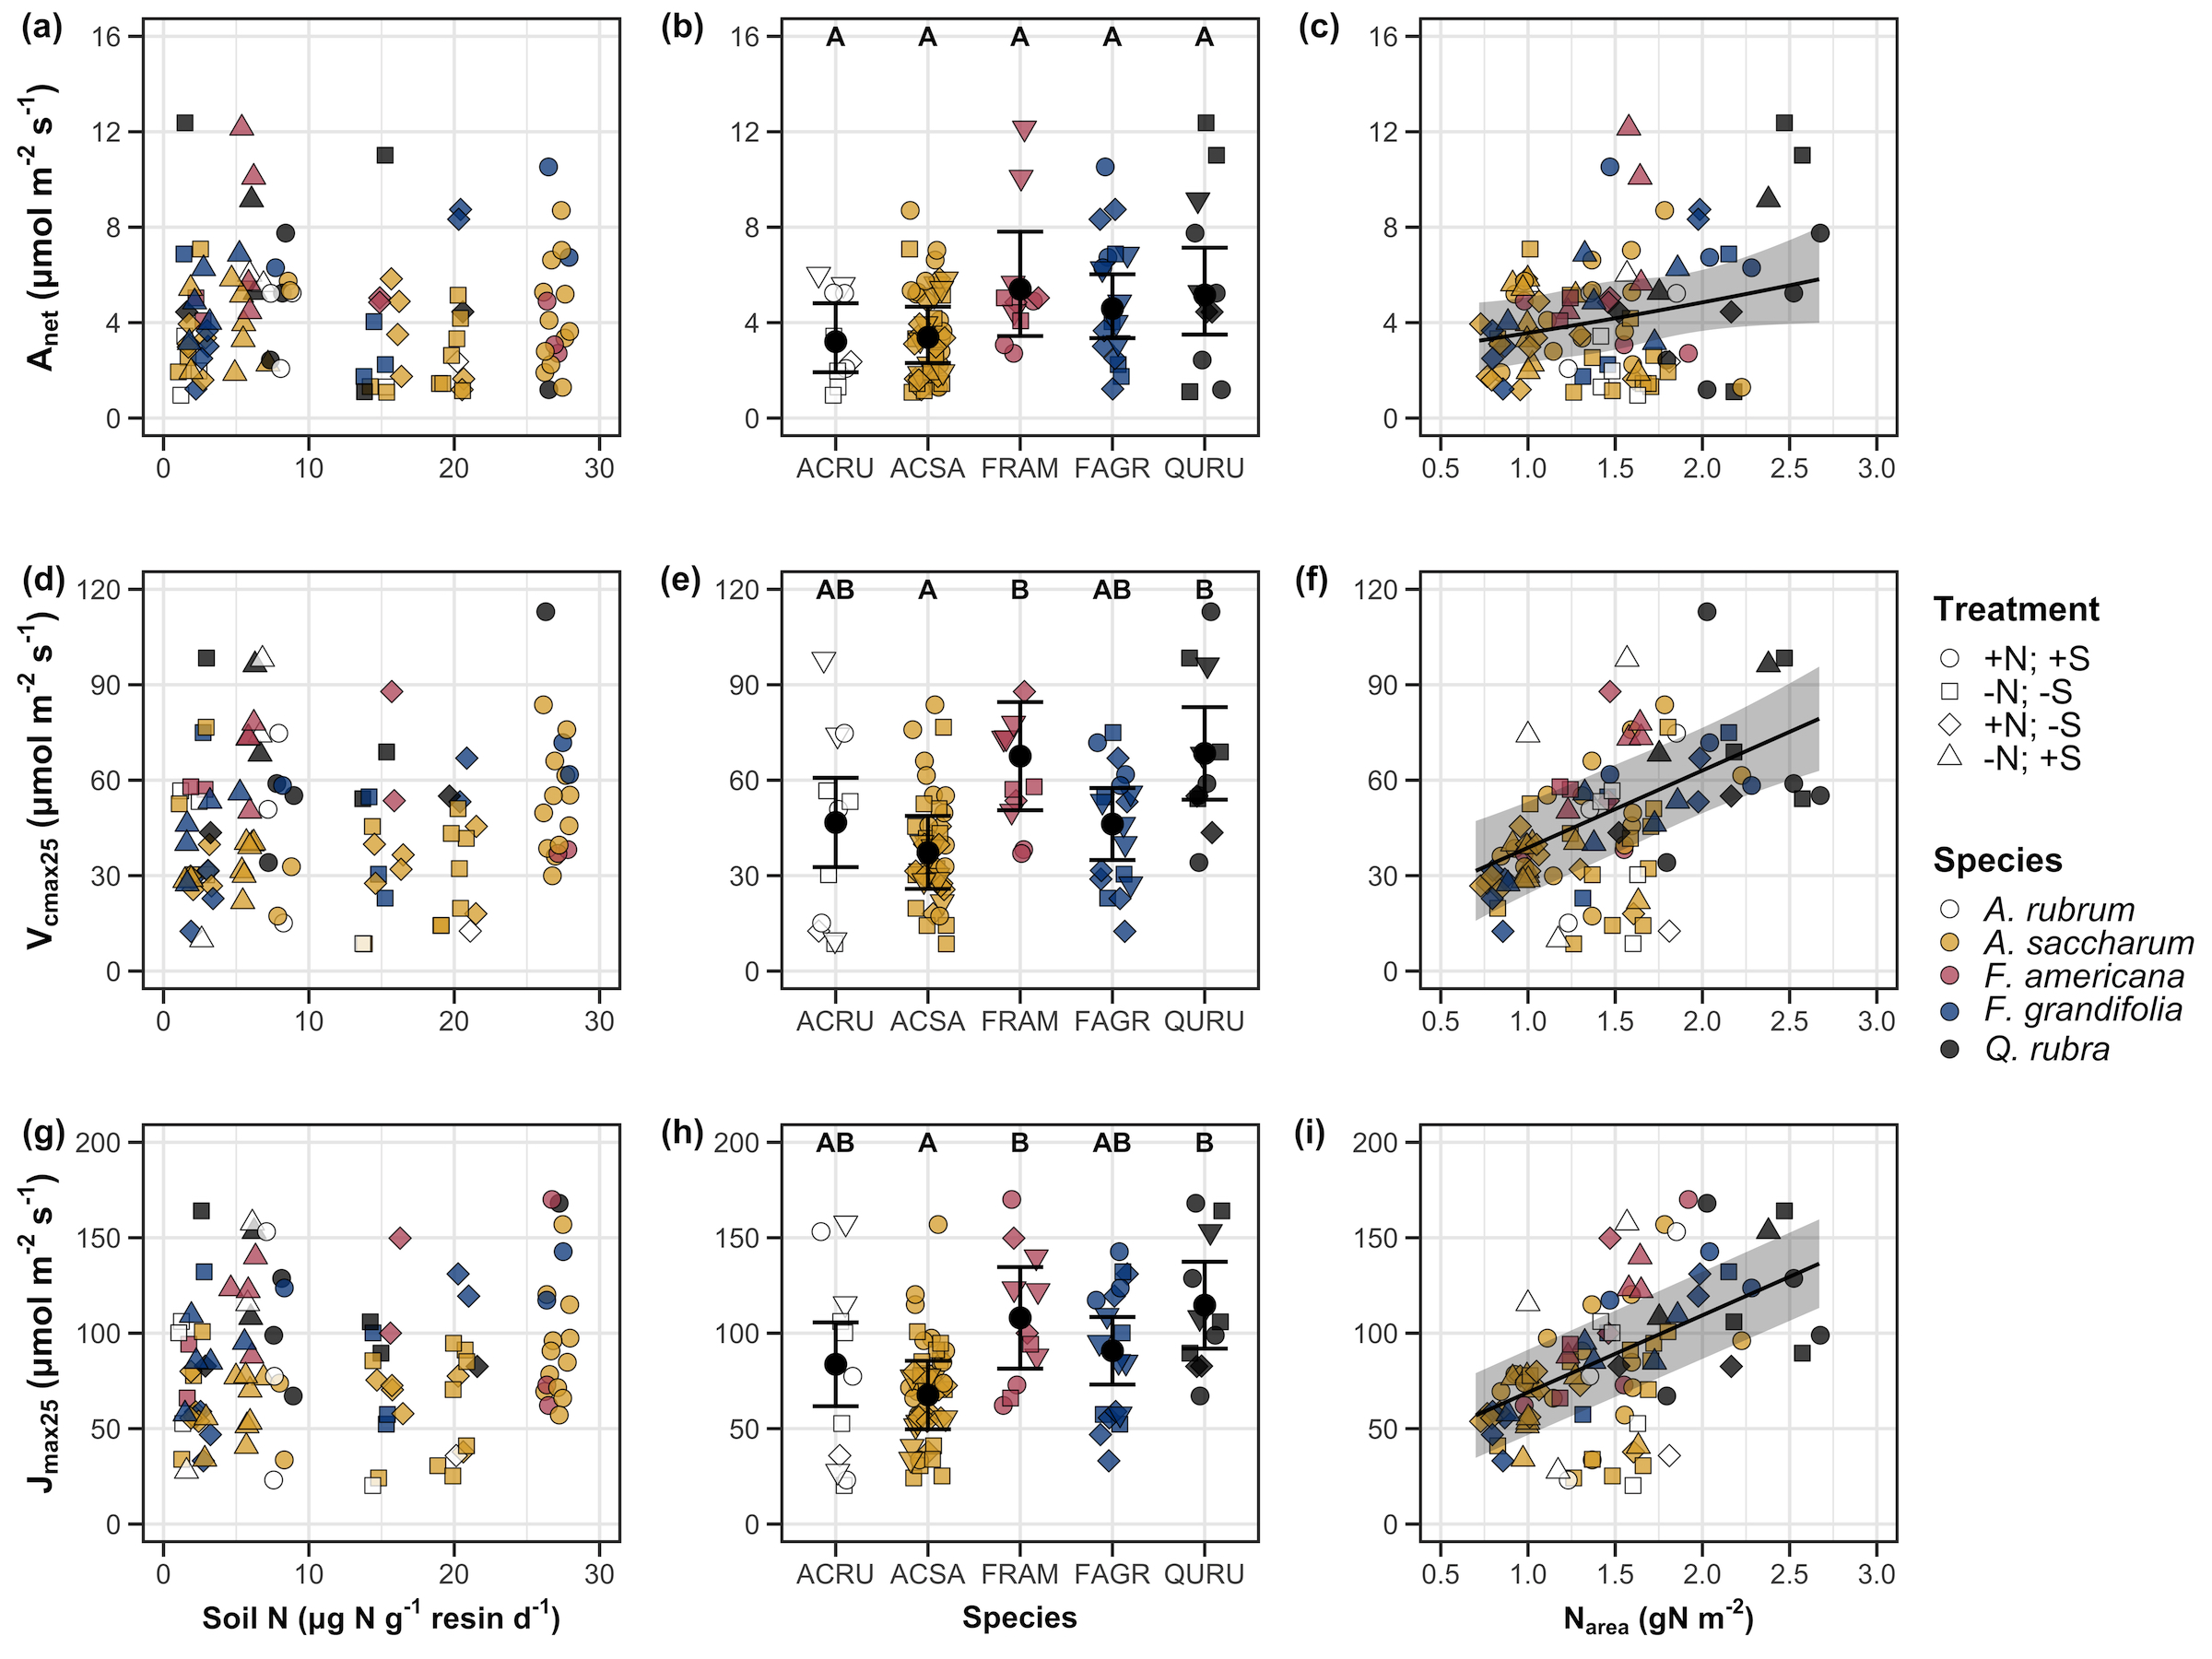
\includegraphics[width=\textwidth]{ch3_NxpH/figs/NxS_fig2_leafbiochem.png}
    \centering
    \caption[Effects of soil nitrogen availability, species, and leaf nitrogen content on net photosynthesis, maximum Rubisco carboxylation rate, and maximum RuBP regeneration rate]{Effects of soil nitrogen availability (left column of panels), species (middle column of panels), and leaf nitrogen content per unit leaf area (right column of panels) on net photosynthesis (a-c), maximum Rubisco carboxylation rate (d-f), and maximum RuBP regeneration rate (g-i). Soil nitrogen availability is represented on the x-axis in the left column of panels, species is represented on the x-axis in the middle column of panels, and leaf nitrogen content per unit leaf area is represented continuously on the x-axis in the right column of panels. Species abbreviations and position along the x-axis in the middle column of panels, colored points, shapes, and trendlines are as explained in Figure \ref{fig:figure3.1}.}
    \label{fig:figure3.2}
\end{figure}
\clearpage

\newpage
\subsection{\textit{Leaf nitrogen allocation}}
\noindent Neither soil nitrogen availability nor soil pH affected the proportion of leaf nitrogen allocated to Rubisco or bioenergetics (Table \ref{tab:table3.3}; Fig. \ref{fig:figure3.3}a, Fig. \ref{fig:figure3.3}c). There was also no effect of soil nitrogen availability or soil pH on the proportion of leaf nitrogen allocated to photosynthesis (Table \ref{tab:table3.3}; Fig. \ref{fig:figure3.3}f). I found no effect of soil nitrogen availability or soil pH on the proportion of leaf nitrogen allocated to structure (Table \ref{tab:table3.3}; Fig \ref{fig:figure3.3}g). Species varied in the proportion of leaf nitrogen allocated to Rubisco, photosynthesis, and structure (Fig \ref{fig:figure3.3}b, Fig. \ref{fig:figure3.3}f, Fig \ref{fig:figure3.3}h), with no detectable species effect on the proportion of leaf nitrogen allocated to bioenergetics (Table \ref{tab:table3.3}, Fig. \ref{fig:figure3.3}d).
\clearpage

\newpage
\begin{landscape}
    \begin{table}
    \centering
    \caption[Effects of soil nitrogen availability, soil pH, and species on the proportion of leaf nitrogen content allocated to photosynthesis, Rubisco, bioenergetics, and structure]{Effects of soil nitrogen availability, soil pH, and species on the proportion of leaf nitrogen content allocated to photosynthesis ($\rho_\mathrm{photo}$; gN gN$^{-1}$), Rubisco ($\rho_\mathrm{rubisco}$; gN gN$^{-1}$), bioenergetics ($\rho_\mathrm{bioe}$; gN gN$^{-1}$), and structure ($\rho_\mathrm{structure}$; gN gN$^{-1}$)$^*$}
    \resizebox{\columnwidth}{!}{
    \begin{tabular}{p{2.5cm}p{0.5cm}p{2cm}p{1.5cm}p{1.5cm}p{2cm}p{1.5cm}p{1.5cm}p{2cm}p{1.5cm}p{1.5cm}}
        && 
        \multicolumn{3}{l}{$\rho_\mathrm{photo}$} 
        & \multicolumn{3}{l}{$\rho_\mathrm{rubisco}$} 
        & \multicolumn{3}{l}{$\rho_\mathrm{bioe}$} 
        \\
        \hline 
        & 
        \multicolumn{1}{r}{df} 
        & \multicolumn{1}{r}{Coefficient} & \multicolumn{1}{r}{$\chi^{2}$} & \multicolumn{1}{r}{\textit{p}} 
        & \multicolumn{1}{r}{Coefficient} & \multicolumn{1}{r}{$\chi^{2}$} & \multicolumn{1}{r}{\textit{p}} 
        & \multicolumn{1}{r}{Coefficient} & \multicolumn{1}{r}{$\chi^{2}$} & \multicolumn{1}{r}{\textit{p}} 
        \\ 
        \hline

        Intercept & \multicolumn{1}{r}{-} 
        &  \multicolumn{1}{r}{4.93E$-$01} & \multicolumn{1}{r}{-} & \multicolumn{1}{r}{-}
        &  \multicolumn{1}{r}{4.17E$-$01} & \multicolumn{1}{r}{-} & \multicolumn{1}{r}{-}
        &  \multicolumn{1}{r}{7.64E$-$02} & \multicolumn{1}{r}{-} & \multicolumn{1}{r}{-} 
        \\

        Soil N & \multicolumn{1}{r}{1}
        & \multicolumn{1}{r}{-1.23E$-$03} & \multicolumn{1}{r}{0.521} & \multicolumn{1}{r}{0.470}
        & \multicolumn{1}{r}{-1.04E$-$03}  & \multicolumn{1}{r}{0.501} & \multicolumn{1}{r}{0.479}
        & \multicolumn{1}{r}{-1.77E$-$04}  & \multicolumn{1}{r}{0.557} & \multicolumn{1}{r}{0.455} 
        \\

        Soil pH & \multicolumn{1}{r}{1}
        & \multicolumn{1}{r}{-4.37E$-$02} & \multicolumn{1}{r}{1.581} & \multicolumn{1}{r}{0.209}
        & \multicolumn{1}{r}{-3.70E$-$02} & \multicolumn{1}{r}{1.511} & \multicolumn{1}{r}{0.219}
        & \multicolumn{1}{r}{-6.84E$-$03} & \multicolumn{1}{r}{1.941} & \multicolumn{1}{r}{0.164} 
        \\

        Species & \multicolumn{1}{r}{4}
        & \multicolumn{1}{r}{-} & \multicolumn{1}{r}{13.106} & \multicolumn{1}{r}{\textbf{0.011}}
        & \multicolumn{1}{r}{-} & \multicolumn{1}{r}{14.152} & \multicolumn{1}{r}{\textbf{0.007}}
        & \multicolumn{1}{r}{-} & \multicolumn{1}{r}{7.300} & \multicolumn{1}{r}{0.121}
        \\

        &&&&&&&&&&
        \\

        && \multicolumn{3}{l}{$\rho_\mathrm{structure}$} &&&&& \\
        \hline
        & \multicolumn{1}{r}{df}
        & \multicolumn{1}{r}{Coefficient} & \multicolumn{1}{r}{$\chi^{2}$} & \multicolumn{1}{r}{\textit{p}} 
        \\
        \hline

        Intercept & \multicolumn{1}{r}{-}
        & \multicolumn{1}{r}{9.77E$-$02} & \multicolumn{1}{r}{-} & \multicolumn{1}{r}{-}
        &&&&&&
        \\

        Soil N & \multicolumn{1}{r}{1}
        & \multicolumn{1}{r}{-2.29E$-$04}  & \multicolumn{1}{r}{1.165} & \multicolumn{1}{r}{0.280}
        &&&&&& 
        \\

        Soil pH & \multicolumn{1}{r}{1}
        & \multicolumn{1}{r}{-1.87E$-$03} & \multicolumn{1}{r}{0.179} & \multicolumn{1}{r}{0.672}
        &&&&&& 
        \\

        Species & \multicolumn{1}{r}{4}
        & \multicolumn{1}{r}{-} & \multicolumn{1}{r}{16.428} & \multicolumn{1}{r}{\textbf{0.002}}
        &&&&&&
        \\
        \hline
    \end{tabular}}
    \label{tab:table3.3}
\end{table}
\begin{singlespace}
    \noindent $^*$Significance determined using Type II Wald $\chi^{2}$ tests ($\alpha$=0.05). \textit{P}-values less than 0.05 are in bold. 
\end{singlespace}
\end{landscape}
\clearpage

\newpage
\begin{figure}
    \includegraphics[scale = 0.049]{ch3_NxpH/figs/NxS_fig3_leafn_allocation.png}
    \centering
    \caption[Effects of soil nitrogen availability, species, and leaf nitrogen content on the fraction of leaf nitrogen allocated to photosynthesis and structure]{Effects of soil nitrogen availability and species on the proportion of leaf nitrogen content allocated to Rubisco (a-b), bioenergetics (c-d), photosynthesis (e-f), and structure (g-h). Soil nitrogen availability is represented on the x-axis in the left column of panels and species are represented on the x-axis in the right column of panels. Species abbreviations and position along the x-axis in the middle column of panels, colored points, shapes, trendlines, error bars, and compact lettering are as explained in Figure \ref{fig:figure3.1}.}
    \label{fig:figure3.3}
    \end{figure}
\clearpage

\newpage
\subsection{\textit{Tradeoffs between nitrogen and water use}}
\noindent Although soil nitrogen availability did not affect $\chi$ (Table \ref{tab:table3.4}; Fig. \ref{fig:figure3.4}a), increasing soil nitrogen availability decreased PNUE (Table \ref{tab:table3.4}; Fig. \ref{fig:figure3.4}d) and increased the ratio of $N_\mathrm{area}$:$\chi$ (Table \ref{tab:table3.4}; Fig. \ref{fig:figure3.4}f). Specifically, this response yielded a 26\% reduction in PNUE and 37\% stimulation in $N_\mathrm{area}$:$\chi$ across the soil nitrogen availability gradient. There was no apparent effect of soil nitrogen availability on $V_\mathrm{cmax25}$:$\chi$ (Table \ref{tab:table3.4}; Fig. \ref{fig:figure3.4}h). Increasing soil pH had a weak marginal negative effect on PNUE, but did not influence $\chi$, $N_\mathrm{area}$:$\chi$, or $V_\mathrm{cmax25}$:$\chi$ (Table \ref{tab:table3.4}). I observed differences in $\chi$ (Fig. \ref{fig:figure3.4}b), PNUE (Fig. \ref{fig:figure3.4}e), $N_\mathrm{area}$:$\chi$ (Fig. \ref{fig:figure3.4}g), and $V_\mathrm{cmax25}$:$\chi$ (Fig. \ref{fig:figure3.4}i) between species (Table \ref{tab:table3.4}). Finally, increasing $N_\mathrm{area}$ had a strong negative effect on $\chi$ (Table \ref{tab:table3.4}; Fig. \ref{fig:figure3.4}c) and a strong positive effect on $V_\mathrm{cmax25}$:$\chi$ (Table \ref{tab:table3.4}; Fig. \ref{fig:figure3.4}j).
\clearpage

\newpage
\begin{landscape}
    \begin{table}
    \centering
    \caption[Effects of soil nitrogen availability, soil pH, species, and $N_\mathrm{area}$ on $\chi$, photosynthetic nitrogen use efficiency, leaf nitrogen content per unit $\chi$, and maximum Rubisco carboxylation rate per unit $\chi$]{Effects of soil nitrogen availability, soil pH, species, and $N_\mathrm{area}$ on $\chi$ (unitless), photosynthetic nitrogen use efficiency (PNUE; $\mathrm{\mu mol\ CO_2\ mol^{-1}\ N\ s^{-1}}$), leaf nitrogen content per unit $\chi$ ($N_\mathrm{area}$:$\chi$; gN m$^{-2}$), and maximum Rubisco carboxylation rate per unit $\chi$ ($V_\mathrm{cmax25}$:$\chi$; $\mathrm{\mu mol\ m^{-2}\ s^{-1}}$)$^*$}
    \resizebox{\columnwidth}{!}{
    \begin{tabular}{p{2.5cm}p{0.5cm}p{2cm}p{1.5cm}p{1.5cm}p{2cm}p{1.5cm}p{1.5cm}p{2cm}p{1.5cm}p{1.5cm}}
        && 
        \multicolumn{3}{l}{$\chi$} 
        & \multicolumn{3}{l}{PNUE} 
        & \multicolumn{3}{l}{$N_\mathrm{area}$:$\chi$} 
        \\
        \hline 
            
        & \multicolumn{1}{r}{df} 
        & \multicolumn{1}{r}{Coefficient} & \multicolumn{1}{r}{$\chi^{2}$} & \multicolumn{1}{r}{\textit{p}} 
        & \multicolumn{1}{r}{Coefficient} & \multicolumn{1}{r}{$\chi^{2}$} & \multicolumn{1}{r}{\textit{p}} 
        & \multicolumn{1}{r}{Coefficient} & \multicolumn{1}{r}{$\chi^{2}$} & \multicolumn{1}{r}{\textit{p}} 
        \\ 
        \hline

        (Intercept) & \multicolumn{1}{r}{-} 
        &  \multicolumn{1}{r}{8.12E$-$01}   & \multicolumn{1}{r}{-} & \multicolumn{1}{r}{-}
        &  \multicolumn{1}{r}{9.57E+00$^\mathrm{b}$}   & \multicolumn{1}{r}{-} & \multicolumn{1}{r}{-}
        &  \multicolumn{1}{r}{9.19E$-$01}   & \multicolumn{1}{r}{-} & \multicolumn{1}{r}{-} 
        \\

        Soil N & \multicolumn{1}{r}{1}
        & \multicolumn{1}{r}{-1.14E$-$03}  & \multicolumn{1}{r}{1.698} & \multicolumn{1}{r}{0.193}
        & \multicolumn{1}{r}{-6.63E$-$02$^\mathrm{b}$}  & \multicolumn{1}{r}{6.396} & \multicolumn{1}{r}{\textbf{0.011}}
        & \multicolumn{1}{r}{2.60E$-$02}   & \multicolumn{1}{r}{9.533} & \multicolumn{1}{r}{\textbf{0.002}} 
        \\


        Soil pH & \multicolumn{1}{r}{1}
        & \multicolumn{1}{r}{-1.91E$-$02}  & \multicolumn{1}{r}{1.087} & \multicolumn{1}{r}{0.297}
        & \multicolumn{1}{r}{-9.25E$-$01$^\mathrm{b}$}  & \multicolumn{1}{r}{2.843} & \multicolumn{1}{r}{\textit{0.092}}
        & \multicolumn{1}{r}{2.03E$-$01}   & \multicolumn{1}{r}{1.321} & \multicolumn{1}{r}{0.250} 
        \\

        Species & \multicolumn{1}{r}{4}
        & \multicolumn{1}{r}{-} & \multicolumn{1}{r}{18.843} & \multicolumn{1}{r}{\textbf{0.001}}
        & \multicolumn{1}{r}{-} & \multicolumn{1}{r}{13.454} & \multicolumn{1}{r}{\textbf{0.009}}
        & \multicolumn{1}{r}{-} & \multicolumn{1}{r}{52.983} & \multicolumn{1}{r}{\textbf{<0.001}}
        \\
        \hline

        ($N_\mathrm{area}$ int.) & \multicolumn{1}{r}{-}
        & \multicolumn{1}{r}{8.93E$-$01}  & \multicolumn{1}{r}{-}    & \multicolumn{1}{r}{-}
        & \multicolumn{1}{r}{-}         & \multicolumn{1}{r}{-}    & \multicolumn{1}{r}{-}
        & \multicolumn{1}{r}{-}         & \multicolumn{1}{r}{-}    & \multicolumn{1}{r}{-}
        \\

        $N_\mathrm{area}$ & \multicolumn{1}{r}{1}
        & \multicolumn{1}{r}{-1.11E$-$01} & \multicolumn{1}{r}{80.606}  & \multicolumn{1}{r}{\textbf{<0.001}}
        & \multicolumn{1}{r}{-}         & \multicolumn{1}{r}{-}       & \multicolumn{1}{r}{-}
        & \multicolumn{1}{r}{-}         & \multicolumn{1}{r}{-}       & \multicolumn{1}{r}{-}
        \\
        \hline

        &&&&&&&&&&
        \\

        && \multicolumn{3}{l}{$V_{\mathrm{cmax25}}$:$\chi$} &&&&& \\
        \hline
        & \multicolumn{1}{r}{df}
        & \multicolumn{1}{r}{Coefficient} & \multicolumn{1}{r}{$\chi^{2}$} & \multicolumn{1}{r}{\textit{p}} 
        \\
        \hline

        (Intercept) & \multicolumn{1}{r}{-}
        & \multicolumn{1}{r}{7.20E+01} & \multicolumn{1}{r}{-} & \multicolumn{1}{r}{-}
        &&&&&&
        \\

        Soil N & \multicolumn{1}{r}{1}
        & \multicolumn{1}{r}{3.99E$-$01}  & \multicolumn{1}{r}{0.963} & \multicolumn{1}{r}{0.326}
        &&&&&& 
        \\

        Soil pH & \multicolumn{1}{r}{1}
        & \multicolumn{1}{r}{-3.12E+00} & \multicolumn{1}{r}{0.138} & \multicolumn{1}{r}{0.711}
        &&&&&& 
        \\

        Species & \multicolumn{1}{r}{4}
        & \multicolumn{1}{r}{-} & \multicolumn{1}{r}{31.450} & \multicolumn{1}{r}{\textbf{<0.001}}
        \\
        \hline

        ($N_\mathrm{area}$ int.) & \multicolumn{1}{r}{-}
        & \multicolumn{1}{r}{1.18E+01} & \multicolumn{1}{r}{-} & \multicolumn{1}{r}{-}
        &&&&&& 
        \\

        $N_\mathrm{area}$ & \multicolumn{1}{r}{4}
        & \multicolumn{1}{r}{3.87E+01} & \multicolumn{1}{r}{32.797} & \multicolumn{1}{r}{\textbf{<0.001}}
        &&&&&
        \\
        \hline
    \end{tabular}}
    \label{tab:table3.4}
    \end{table}
\begin{singlespace}
    \noindent $^*$Significance determined using Type II Wald $\chi^{2}$ tests ($\alpha$ = 0.05). \textit{P}-values less than 0.05 are in bold, while \textit{p}-values between 0.05 and 0.1 are italicized. Superscript letters indicate model coefficients fit to natural-log ($^\mathrm{a}$) or square-root ($^\mathrm{b}$) transformed data. Relationships between $N_\mathrm{area}$ and each response variable were fit using the second series of bivariate mixed-effects models, so model coefficients and results are independent of model coefficients and results reported for relationships between soil nitrogen, soil pH, and species for each response variable.
\end{singlespace}
\end{landscape}
\clearpage

\newpage
\begin{figure}
    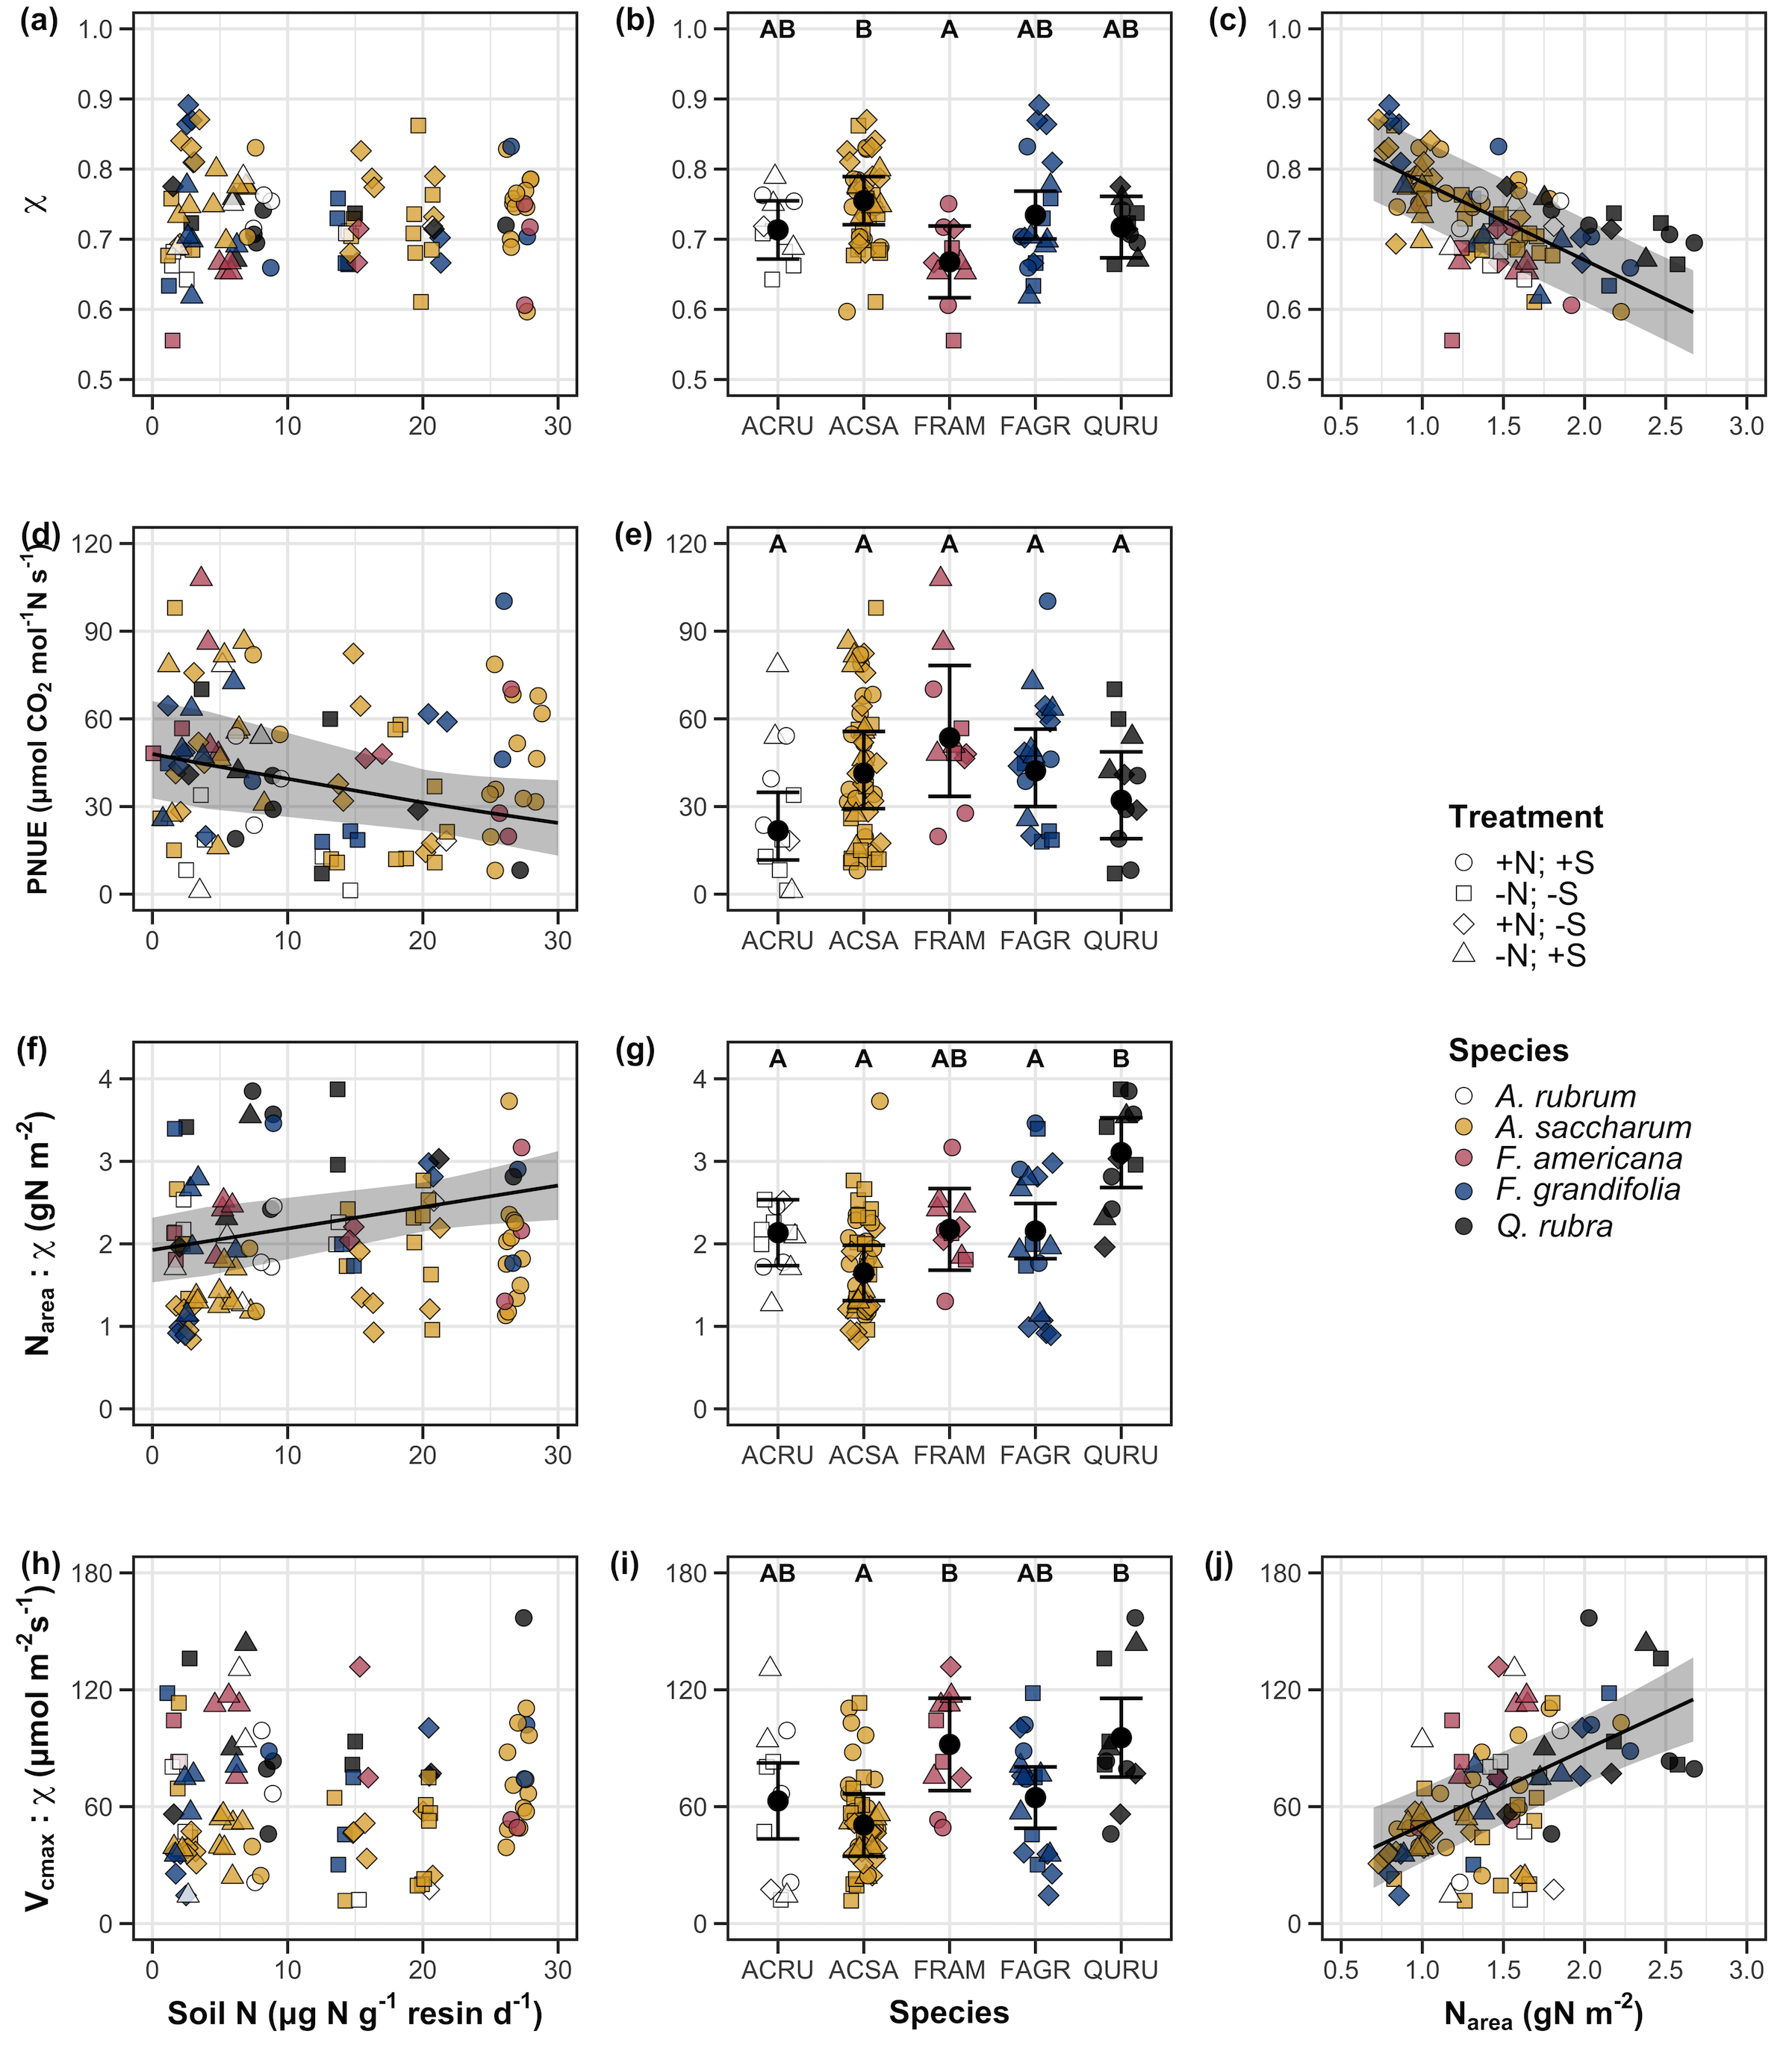
\includegraphics[width=\textwidth]{ch3_NxpH/figs/NxS_fig4_pnueiwue.png}
    \centering
    \caption[Effects of soil N availability, species, and leaf N content on tradeoffs between nitrogen and water use]{Effects of soil nitrogen availability and species on the proportion of leaf nitrogen content allocated to Rubisco (a-b), bioenergetics (c-d), photosynthesis (Rubisco + bioenergetics; e-f), and structure (g-h). Soil nitrogen availability is represented on the x-axis in the left column of panels and species are represented on the x-axis in the right column of panels. Species abbreviations and position along the x-axis in the middle column of panels, colored points, shapes, trendlines, error bars, and compact lettering are as explained in Figure \ref{fig:figure3.1}.}
    \label{fig:figure3.4}
\end{figure}
\clearpage

\section{Discussion}
\noindent Photosynthetic least-cost theory provides an explanation for understanding relationships between soil nutrient availability, leaf nutrient allocation, and photosynthetic capacity. The theory suggests that plants acclimate to a given environment by optimizing leaf photosynthesis rates at the lowest summed cost of using nutrients and water \shortcite{Prentice2014,Wang2017,Smith2019,Paillassa2020}. The theory predicts that an increase in soil nutrient availability should allow similar photosynthesis rates to be achieved with increased leaf nutrient content and photosynthetic capacity (i.e., $V_\mathrm{cmax25}$ and $J_\mathrm{max25}$) at lower leaf $C_\mathrm{i}$:$C_\mathrm{a}$ ($\chi$), resulting in an increase in water use efficiency, decrease in nutrient use efficiency, and increase in both leaf nutrient content and photosynthetic capacity per unit $\chi$. The theory predicts similar leaf responses to increasing soil pH under acidic conditions, presumably due to generally faster nutrient cycle dynamics and consequent reductions in the cost of acquiring nutrients relative to water with increasing soil pH \shortcite{Wang2017,Paillassa2020,Dong2020}.
    
Supporting the theory, increasing soil nitrogen availability was associated with increased leaf nitrogen content, a pattern that reduced photosynthetic nitrogen use efficiency and increased leaf nitrogen content per unit $\chi$. Increasing soil nitrogen coincided with slight, but non-significant decreases in $\chi$ and increases in $V_\mathrm{cmax25}$ and $J_\mathrm{max25}$ (\textit{p}<0.2, Table \ref{tab:table3.2}). The positive trend between soil nitrogen availability and photosynthetic capacity was supported by the concurrent strong increase in leaf nitrogen content with increasing soil nitrogen availability, which resulted in no change in the proportion of leaf nitrogen content allocated to photosynthesis across the soil nitrogen availability gradient. Additionally, leaf nitrogen content exhibited a strong negative correlation with $\chi$, indicative of strong nitrogen-water use tradeoffs at the leaf level. Responses tended to vary more due to soil nitrogen availability than soil pH. Overall, these findings are consistent with the nutrient-water use tradeoffs predicted from theory.

\subsection{\textit{Soil nitrogen availability modifies tradeoffs between nitrogen and water use}}
\noindent In support of expected least-cost outcomes and past environmental gradient studies \shortcite{Dong2017,Paillassa2020}, increasing soil nitrogen availability was associated with increased leaf nitrogen content. Soil nitrogen availability had smaller impacts on measures of net photosynthesis and $\chi$, which led to reductions in PNUE and increases in leaf nitrogen content per unit $\chi$, as expected from theory. Photosynthetic least-cost theory suggests that reductions in PNUE should be driven by an increase in the proportion of leaf nitrogen allocated to photosynthetic tissue, a pattern that should allow plants to achieve optimal photosynthetic rates with greater photosynthetic capacity to make better use of available light. Contrasting theory predictions, I found no effect of soil nitrogen availability on photosynthetic capacity. However, photosynthetic capacity did tend to increase with increasing soil nitrogen availability (\textit{p}<0.20; Table \ref{tab:table3.2}) resulting in no effect of soil nitrogen availability on the relative fraction of leaf nitrogen allocated to photosynthesis, Rubisco, or bioenergetics. These lines of evidence support the idea that trees use additional nitrogen to support increased leaf nitrogen allocation toward photosynthetic tissue and enhance photosynthetic capacity \shortcite{Wright2003}.

Soil nitrogen availability had a stronger effect on leaf nitrogen than photosynthetic capacity. This pattern suggests that additional plant nitrogen uptake due to increased soil nitrogen availability was also being used to support non-photosynthetic nitrogen pools, possibly to structural tissue or stress-induced amino acid and polyamine synthesis \shortcite{Minocha2000,Onoda2004,Bubier2011}. While I found no change in the proportion of leaf nitrogen allocated to leaf structural tissue, the overall stimulation in leaf nitrogen content with increasing soil nitrogen availability suggests an increase in the net amount of nitrogen invested in leaf structural tissue along the nitrogen availability gradient. Importantly, leaf nitrogen allocated to structure was calculated using an empirical relationship between $M_\mathrm{area}$ and the amount of leaf nitrogen allocated to cell walls \shortcite{Onoda2017}. As the generality of relationships between $M_\mathrm{area}$ and the amount of leaf nitrogen allocated to cell walls has been called into question \shortcite{Harrison2009}, future work should consider explicitly measuring nitrogen allocation to cell wall tissue and stress-induced amino acid synthesis to confirm these patterns.
    
In opposition to patterns expected from least-cost theory, increasing soil nitrogen availability had no apparent effect on $\chi$. Interestingly, despite the null effect of soil nitrogen availability on $\chi$, I observed a strong negative effect of increasing $N_\mathrm{area}$ on $\chi$, consistent with the nitrogen-water use tradeoffs expected from theory. The null response of $\chi$ to increasing soil nitrogen availability may have been due to a lack of water limitation in the system, given that the area received approximately 20\% more precipitation (1167 mm) during the 12-month period leading up to our measurement period than normally expected (972 mm). However, droughts can and do occur in temperate forests of the northeastern United States \shortcite{Sweet2017}, so the observed increase in leaf nitrogen content with increasing soil nitrogen availability could be a strategy that allows trees to hedge bets against drier than normal growing seasons \shortcite{Onoda2004,Onoda2017,Hallik2009}. As was suggested in \shortciteN{Paillassa2020}, and more recently by \shortciteN{Querejeta2022}, negative effects of soil nitrogen availability on $\chi$ may increase with increasing aridity. This strategy would be especially advantageous if it allows individuals growing in arid regions to maintain carbon assimilation rates with reduced water loss. Future work should attempt to quantify interactive roles of climate and soil nitrogen availability on nitrogen-water use tradeoffs, which could be done by leveraging coordinated and multifactor nutrient \shortcite{Borer2014} and water \shortcite{Knapp2017} manipulation experiments across broad climatic gradients.
    
\subsection{\textit{Soil pH did not modify tradeoffs between nitrogen and water usage}}
\noindent While the primary purpose of this study was to examine the role of soil nitrogen availability on nitrogen-water use tradeoffs, this experimental design manipulated both soil nitrogen and pH, providing an opportunity to isolate the roles of these variables. Previous correlational studies along environmental gradients have identified soil pH as a particularly important factor that can modify tradeoffs between nutrient and water use \shortcite{Smith2019,Paillassa2020,Westerband2023} and the proportion of leaf nitrogen allocated to photosynthesis \shortcite{Luo2021}. Such studies implied that these patterns may be driven by reductions in the cost of acquiring nutrients relative to water with increasing pH, which may be exacerbated in acidic soils.

Consistent with theory \shortcite{Wright2003,Prentice2014}, results indicate that increasing soil pH was negatively associated with PNUE. However, there was no effect of soil pH on leaf nitrogen content, $\chi$, or leaf nitrogen content per unit $\chi$, most likely because the experimental nitrogen additions increased soil nitrogen supply while both increasing (sodium nitrate) and decreasing (ammonium sulfate) soil pH. These results suggest that soil pH did not play a major role in modifying expected photosynthetic least-cost theory patterns, contrasting findings from \shortciteN{Paillassa2020} and other gradient studies that note positive effects of increasing soil pH on leaf nitrogen content, Rubisco carboxylation, and $\chi$ \shortcite{Viet2013,Cornwell2018,Luo2021}. Instead, null responses to soil pH show that leaf photosynthetic parameters depend more on soil nitrogen availability than pH per se, and that inferences from gradient studies might be confounding covariation between nitrogen availability and soil acidity.

\subsection{\textit{Species identity explains a large amount of variation in leaf and whole plant traits}}
\noindent Species generally explained a larger amount of variation in measured leaf traits than soil nitrogen availability or soil pH. Interspecies variation is an important factor to consider when deducing mechanisms that drive photosynthetic least-cost theory, particularly for species that form distinct mycorrhizal associations or have different photosynthetic pathways, growth forms, or leaf habit \shortcite{Espelta2005,Adams2016,BialicMurphy2021,Scott2022}. The need to consider species may also be important when comparing nutrient-water use tradeoffs in early and late successional species, or in species with different resource economic strategies \shortcite{Abrams1995,Ellsworth1996,Wright2004,Reich2014,Onoda2017,Ziegler2020}.
    
A strength of the study design and sampling effort is that it controls for many species differences that should modify nitrogen-water use tradeoffs expected from theory. All tree species measured in this study shared the leaf habit of deciduous broadleaves, were growing in forests of similar successional stage, but differed in mycorrhizal association and consequent resource economic strategies. As stands tended to be dominated by trees that associate with arbuscular mycorrhizae (\textit{Fraxinus} and both \textit{Acer} species made up roughly 70\% of total aboveground biomass across stands), ecosystem biogeochemical cycle dynamics may be more closely aligned to the inorganic nutrient economy proposed in \shortciteN{Phillips2013}, which may promote stronger nitrogen-water use tradeoffs in tree species that associate with arbuscular mycorrhizae. This result was not observed here, as photosynthetic properties varied as much within as across the two mycorrhizal associations represented. Given the high variability in measured photosynthetic traits within and across species, effects of mycorrhizal association likely require more intensive sampling efforts to detect than were possible here.
    
\subsection{\textit{Implications for photosynthetic least-cost theory model development}}
\noindent In the field, soil nutrient availability is heterogeneous across time and space (Table \ref{tab:table.b4}). Unaccounted within-plot heterogeneity may have contributed to the low amount of variation explained by soil nitrogen availability in statistical models, as resin bags are a coarse surrogate for soil nitrogen availability. Despite this, I still observed evidence for nutrient-water use tradeoffs, suggesting that observed responses reported here may be an underestimate toward the net effect of soil nitrogen availability on these tradeoffs. While I urge caution in the interpretation of these results, they do provide a promising baseline for future studies investigating patterns expected from photosynthetic least-cost theory at finer spatiotemporal resolutions.
    
The general stronger relationship between leaf nitrogen content and photosynthetic parameters versus between leaf nitrogen content and soil nitrogen availability suggests that leaf nitrogen content is more directly tied to photosynthesis than soil nitrogen availability. While this could be due to the high spatiotemporal heterogeneity of soil nitrogen availability, principles from photosynthetic least-cost theory suggest that leaf nitrogen content is the downstream product of leaf nutrient demand to build and maintain photosynthetic machinery, which is set by aboveground environmental conditions such as light availability, CO$_2$, temperature, or vapor pressure deficit \shortcite{Smith2019,Paillassa2020,Peng2021,Westerband2023}. The stronger relationship between leaf nitrogen and photosynthetic parameters, paired with the strong negative relationship between leaf nitrogen and $\chi$, could indicate a relatively stronger effect of climate on leaf nitrogen-photosynthesis relationships than soil resource availability. However, the short distance between plots and across sites limited my ability to test this mechanism.
    
Variation in soil pH affected least cost responses less than variations in soil nitrogen availability, in part because experimental treatments directly increased soil nitrogen and affected soil pH in opposite directions. While soil pH has been shown to drive nitrogen-water tradeoffs in global gradient analyses \shortcite{Viet2013,Paillassa2020}, these responses may be due to covariations between soil pH and nutrient cycling rather than a role of pH per se. The direct manipulations of soil pH and soil nitrogen availability in this study partly disentangle these factors and show that variation in nitrogen availability matters more for least-cost tradeoffs than pH alone.

\subsection{\textit{Conclusions}}
\noindent Increasing soil nitrogen availability generally increased leaf nitrogen content (both area- and mass-based), but did not significantly influence $\chi$. This shift in leaf nitrogen led to a reduction in PNUE, and an increase in leaf nitrogen per unit $\chi$ with increasing soil nitrogen availability. Despite null effects of soil nitrogen availability on $\chi$, I observed a strong negative relationship between leaf nitrogen content and $\chi$. These results provide empirical support for the nutrient-water use tradeoffs expected from photosynthetic least-cost theory in response to increasing soil nutrient availability, but suggest that all tenets of the theory may not hold in every environment. These results experimentally test previous work suggesting that leaf nitrogen-water economies vary across gradients of soil nutrient availability and pH, and show that variations in nutrient availability matter more for determining variation in leaf photosynthetic traits than soil pH.


%%%%%%%%%%%%%%%%%%%%%%%%%%%%%%%%%%%%%%%%%%%%%%%%%%
%%%%%%%%%%%%%%%%%%%%%%%%%%%%%%%%%%%%%%%%%%%%%%%%%%
%%%%%%%%%%%%%%%%%%%%%%%%%%%%%%%%%%%%%%%%%%%%%%%%%%
%Start TX ecolab experiment chapter              %
%%%%%%%%%%%%%%%%%%%%%%%%%%%%%%%%%%%%%%%%%%%%%%%%%%
%%%%%%%%%%%%%%%%%%%%%%%%%%%%%%%%%%%%%%%%%%%%%%%%%%
%%%%%%%%%%%%%%%%%%%%%%%%%%%%%%%%%%%%%%%%%%%%%%%%%%
\begin{singlespace}
    \chapter{\textbf{The relative cost of resource use for photosynthesis drives variance in leaf nitrogen content across climate and soil resource availability gradients}}
\end{singlespace}

\section{Introduction}
Terrestrial biosphere models, which comprise the land surface component of Earth system models, are sensitive to the formulation of photosynthetic processes \shortcite{Knorr2000,Ziehn2011,Booth2012}. This is because photosynthesis is the largest carbon flux between the atmosphere and terrestrial biosphere, and is constrained by ecosystem carbon and nutrient cycles \shortcite{Hungate2003,LeBauer2008,IPCC2021,Fay2015}. Many terrestrial biosphere models formulate photosynthesis by parameterizing photosynthetic capacity within plant functional groups through empirical linear relationships between area-based leaf nitrogen content ($N_\mathrm{area}$) and the maximum carboxylation rate of Ribulose-1,5-bisphosphate carboxylase/oxygenase \shortcite{Kattge2009,Rogers2014,Rogers2017a}. Models are also beginning to include connected carbon-nitrogen cycles \shortcite{Wieder2015_NPP,Shi2016,Davies-Barnard2020,Braghiere2022}, which allows leaf photosynthesis to be predicted directly through changes in $N_{\mathrm{area}}$ and indirectly through changes in soil nitrogen availability (e.g., LPJ-GUESS, Smith et al., 2014; CLM5.0, Lawrence et al., 2019). Despite recent model developments, open questions remain regarding the generality of ecological relationships between soil nitrogen availability, leaf nitrogen content, and leaf photosynthesis across edaphic and climatic gradients.

Empirical support for positive relationships between soil nitrogen availability and $N_\mathrm{area}$ is abundant \shortcite{Firn2019,Liang2020}, and is a result often attributed to the high nitrogen cost of building and maintaining Rubisco \shortcite{Evans1989_photoN,EvansSeemann1989,Onoda2004,Onoda2017,Dong2020}. Such patterns imply that positive relationships between soil nitrogen availability and $N_\mathrm{area}$ should cause an increase in leaf photosynthesis and photosynthetic capacity by increasing the maximum rate of Rubisco carboxylation through increased investments to Rubisco construction and maintenance. This integrated $N_\mathrm{area}$-photosynthesis response to soil nitrogen availability has been observed both in manipulative experiments and across environmental gradients \shortcite{Field1986,Evans1989_photoN,Walker2014,Li2020}, and is thought to be driven by ecosystem nitrogen limitation, which limits primary productivity globally \shortcite{LeBauer2008,Fay2015}. However, this response is not consistently observed, as recent studies note variable $N_\mathrm{area}$-photosynthesis relationships across soil nitrogen availability gradients \shortcite{Liang2020,Luo2021} and that aboveground growing conditions (e.g., light availability, temperature, vapor pressure deficit) or species identity traits (e.g., photosynthetic pathway, nitrogen acquisition strategy) may be more important for explaining variance in $N_\mathrm{area}$ and photosynthetic capacity across time and space \shortcite{Adams2016,Dong2017,Dong2020,Dong2022a,Smith2019,Peng2021,Westerband2023}.

One hypothesized mechanism to explain variance in $N_\mathrm{area}$ across environmental gradients has been proposed via photosynthetic least-cost theory \shortcite{Wright2003,Prentice2014,Paillassa2020,Harrison2021}. The theory predicts that plants acclimate to environments by optimizing photosynthetic assimilation rates at the lowest summed cost of nitrogen and water use \shortcite{Wright2003,Prentice2014}. In a given environment, the theory proposes that nitrogen and water use can be substituted for each other to maintain the lowest summed cost to satisfy leaf resource demand, such that optimal photosynthetic rates are achieved with less efficient use of the more abundant and less costly resource to acquire in exchange for more efficient use of the less abundant and more costly resource to acquire. 

Photosynthetic least-cost theory predicts that, all else equal, an increase in soil nitrogen availability should decrease the cost of acquiring and using nitrogen relative to water ($\beta$), resulting in optimal photosynthetic rates achieved with greater $N_\mathrm{area}$ at lower stomatal conductance and lower leaf C\textsubscript{i}:C\textsubscript{a} ($\chi$) \shortcite{Wright2003,Prentice2014}. Alternatively, an increase in soil moisture should reduce costs of water acquisition and use, increasing $\beta$, stomatal conductance, and $\chi$, resulting in optimal photosynthetic rates achieved with decreased $N_\mathrm{area}$. The theory also predicts variability in stomatal conductance and $N_\mathrm{area}$ in response to climatic factors, suggesting that the optimal response to increased vapor pressure deficit (VPD) should be a reduction in stomatal conductance and $\chi$ that is counterbalanced by an increase in $N_\mathrm{area}$ to support the higher photosynthetic capacity needed to maintain high assimilation at lower conductance \shortcite{Grossiord2020,Dong2020,Westerband2023}.

Leaf nitrogen allocation responses to changing climates or soil resource availability may also depend on their mode of nutrient acquisition or photosynthetic pathway. For example, species that form associations with symbiotic nitrogen-fixing bacteria (referred as “N-fixing species” from this point forward) should, in theory, have access to a less finite nitrogen supply, which may result in lower $\beta$ values than species not capable of forming such associations (referred as “non-fixing species” from this point forward). This result was previously shown in a greenhouse experiment, where a leguminous species generally had lower costs of nitrogen acquisition compared to a non-leguminous species, although these differences were generally stronger under increased nitrogen limitation (Fig. \ref{fig:figure2.1}) \shortcite{Perkowski2021}. Lower $\beta$ values could be a possible explanation for why N-fixing species commonly have higher leaf nitrogen content than non-fixing species \shortcite{Adams2016,Dong2017}. 

Similarly, leaf nitrogen allocation patterns across environmental gradients may be dependent on photosynthetic pathway. General lower $\chi$ values in C$_4$ species suggests that C$_4$ species should have lower $\beta$ values than C$_3$ species, a pattern that could be the result of increased costs associated with water acquisition and use or reduced costs associated with nutrient acquisition and use relative to C$_3$ species. No study to date has directly quantified $\chi$ in C$_4$ species aside from the dataset used to initially parameterize an optimality model for C$_4$ species \shortcite{Scott2022}.

While photosynthetic least-cost theory provides a unified hypothesis for understanding effects of climate and soil resource availability on $N_\mathrm{area}$, empirical tests of the theory are sparse. Increasing soil nitrogen availability has been previously shown to decrease the cost of acquiring nutrients \shortcite{Bae2015,Lu2022,Eastman2021}, which can induce predictable nutrient-water use tradeoffs expected from the theory across broad environmental gradients \shortcite{Paillassa2020,Querejeta2022,Westerband2023} and in manipulation experiments \shortcite{BialicMurphy2021}. Additionally, increasing VPD has been shown to have a positive effect on $N_\mathrm{area}$ \shortcite{Dong2017,Dong2020,Firn2019}. However, studies have been restricted to exploring these patterns with C$_3$ species and, while previous studies have shown that variance in $N_\mathrm{area}$ across environmental gradients is driven by strong negative relationships with $\chi$ (Fig \ref{fig:figure3.4}c)\shortcite{Dong2017,Paillassa2020,Westerband2023}, no study to date has explicitly investigated effects of soil resource availability or plant functional group on $N_\mathrm{area}$ using $\beta$ as a direct predictor of $\chi$. Additionally, as $N_\mathrm{area}$ can be broken down into structural (leaf mass per area; $M_\mathrm{area}$; $\mathrm{g\ m^{-2}}$) and metabolic (mass-based leaf nitrogen content; $N_\mathrm{mass}$; $\mathrm{g N\ g^{-1}}$) components (Dong et al. 2017), no study has investigated which component of $N_\mathrm{area}$ drives the hypothesized response of $N_\mathrm{area}$ to $\chi$, which would be useful for detecting whether changes in $N_\mathrm{area}$ due to $\chi$ are driven by changes in leaf morphology or stoichiometry.

Here, I measured $N_\mathrm{area}$, $N_\mathrm{mass}$, $M_\mathrm{area}$, leaf $\delta^{13}$C-derived estimates of $\chi$, and leaf $\delta^{13}$C-derived estimates of $\beta$ in 520 individuals spanning 57 species scattered across 24 grassland sites in Texas, USA (Table S1). Texas contains a diverse climatic gradient, indicated by 2006-2020 mean annual precipitation totals ranging from 204 to 1803 mm and 2006-2020 mean annual temperature ranging from 11.8\textdegree{} to 24.6\textdegree{}C. Variability in soil nitrogen availability and soil moisture was expected across sites, owing to differences in soil texture and aboveground climate that would drive differential rates of water retention and nitrogen transformations to plant-available substrate. I leveraged the expected climatic and soil resource variability across sites to test the following hypotheses:

\begin{enumerate}
    \item Soil nitrogen availability will decrease $\beta$ through a reduction in costs of nitrogen acquisition and use, while soil moisture will increase $\beta$ through a reduction in costs of water acquisition and use. We expected that N-fixing species would have lower $\beta$ values due to their ability to minimize costs of nitrogen acquisition under low nitrogen availability and that C$_4$ species would have lower $\beta$ values due to increased costs of water acquisition and use or reduced costs of nitrogen acquisition and use.
    
    \item $\chi$ will be positively related to $\beta$, a pattern that will result in a negative indirect effect of increasing soil nitrogen availability, positive indirect effect of increasing soil moisture on $\chi$, and lower $\chi$ in both N-fixing species and C$_4$ species. We also expected that $\chi$ would be negatively related to VPD, as increasing atmospheric dryness should cause plants to close stomata to minimize water loss.

    \item $N_\mathrm{area}$ will be negatively related to $\chi$. This response will result in an indirect positive effect of increasing soil nitrogen availability, a negative effect of increasing soil moisture on $N_\mathrm{area}$, and generally larger $N_\mathrm{area}$ values in both N-fixing species. We expected these patterns to be mediated through a positive relationship between $\beta$ and $\chi$. While theory predicts that negative relationships between $N_\mathrm{area}$ and $\chi$ should yield generally larger $N_\mathrm{area}$ in C$_4$ species, we expected that C$_4$ species would have lower $N_\mathrm{area}$ due to generally greater nitrogen use efficiency in C$_4$ species than C$_3$ species. Additionally, VPD was expected to increase $N_\mathrm{area}$, a pattern that would be directly mediated through the reduction in $\chi$ with increasing VPD.
\end{enumerate}

\section{Methods}
\subsection{\textit{Site descriptions and sampling methodology}}
I collected leaf and soil samples from 24 open grassland sites across central and eastern Texas in summer 2020 and summer 2021 (Fig. \ref{fig:figure4.1}). Twelve sites were visited between June and July 2020 and 14 sites (11 unique from 2020) were visited between May and June 2021 (Table 1). I explicitly chose sites that maximized variability in precipitation and edaphic variability between sites while minimizing temperature variability across the environmental gradient (Table 1). No site with personally communicated or anecdotal evidence of grazing or disturbance (e.g., mowing, feral hog activity, etc.) were used. I collected leaf material from three individuals each of the five most abundant species at random locations at each site, only  selecting species that were broadly classified as graminoid or forb/herb growth habits per the USDA PLANTS database \shortcite{USDANRCS2022}. All collected leaves were fully expanded with no visible herbivory or other external damage and also free from shading by nearby shrubs or trees. Five soil samples were collected from 0-15cm below the soil surface at each site near the leaf collection sample locations. Soil samples were later mixed together by hand to create one composite soil sample per site.

\subsection{\textit{Leaf trait measurements}}
Images of each leaf were taken immediately following each site visit using a flat-bed scanner. Fresh leaf area was determined from each image using the 'LeafArea' R package \shortcite{Katabuchi2015}, which automates leaf area calculations using ImageJ software \shortcite{Schneider2012}. Each leaf was dried at 65\textdegree{}C for at least 48 hours to a constant mass, weighed, and manually ground in a mortar and pestle until homogenized. Leaf mass per area ($M_\mathrm{area}$; $\mathrm{g\ m^{-2}}$) was calculated as the ratio of dry leaf biomass to fresh leaf area. Subsamples of dried and homogenized leaf tissue were used to measure leaf nitrogen content ($N_\mathrm{mass}$; $\mathrm{gN\ g^{-1}}$) through elemental combustion analysis (Costech-4010, Costech Instruments, Valencia, CA). Leaf nitrogen content per unit leaf area ($N_area$; $\mathrm{gN\ m^{-2}}$) was then calculated as the product of $N_\mathrm{mass}$ and $M_\mathrm{area}$.
    
Subsamples of dried and homogenized leaf tissue were sent to the University of California-Davis Stable Isotope Facility to determine leaf $\delta^{13}$C. Leaf $\delta^{13}$C values were determined using an elemental analyzer (PDZ Europa ANCA-GSL; Sercon Ltd., Chestshire, UK) interfaced to an isotope ratio mass spectrometer (PDZ Europa 20-20 Isotope Ratio Mass Spectrometer, Sercon Ltd., Chestshire, UK). I used leaf $\delta^{13}$C values (‰; relative to Vienna Pee Dee Belemnite international reference standard) to estimate the ratio of intercellular ($C_\mathrm{i}$) to extracellular ($C_\mathrm{a}$) CO\textsubscript{2} ratio (leaf $C_\mathrm{i}$:$C_\mathrm{a}$, $\chi$; unitless) following the approach of Farquhar et al. (1989) described in Cernusak et al. (2013). Specifically, I derived $\chi$ as:

\begin{equation} 
    \label{eq_4.1}
    \chi=\frac{C_{i}}{C_{a}}=\frac{\Delta^{13}C - a}{b - a}
\end{equation}
    
\noindent where $\Delta^{13}$C represents the relative difference between leaf $\delta^{13}$C (‰) and air $\delta^{13}$C (‰), and is calculated as:

\begin{equation}
    \label{eq_4.2}
    \Delta^{13}C = \frac{\delta^{13}C_{air} - \delta^{13}C_{leaf}}{1 + \delta^{13}C_{leaf}}
\end{equation}

\noindent $\delta^{13}\mathrm{C_{air}}$, traditionally assumed to be -8‰ \shortcite{Keeling1979,Farquhar1989}, was calculated as a function of calendar year \textit{t} using an empirical equation derived in \shortciteN{Feng1999}:

\begin{equation}
    \label{eq_4.3}
    \delta^{13}C_{air} = -6.429 - 0.006e^{0.0217(t-1740)}
\end{equation}
    
 \noindent This calculation resulted in $\delta^{13}\mathrm{C_{air}}$ values for 2020 and 2021 as -9.04 and -9.09, respectively. a represents the fractionation between $^{12}\mathrm{C}$ and $^{13}\mathrm{C}$ due to diffusion in air, assumed to be 4.4‰, and b represents the fractionation caused by Rubisco carboxylation, assumed to be 27‰ \shortcite{Farquhar1989}. For $C_{4}$ species, b in Eqn. \ref{eq_4.1} was set to 6.3‰, and was derived from:

\begin{equation}
    \label{eq_4.4}
    b = c + (d \cdot \phi)
\end{equation}
    
\noindent Where c was set to -5.7‰ and d was set to 30‰ \shortcite{Farquhar1989}. $\phi$, which is the bundle sheath leakiness term, was set to 0.4. All $\chi$ values less than 0.2 and greater than 1.0 were assumed to be incorrect and removed.
    
I derived the unit cost of resource use ($\beta$) using leaf $\chi$ and site climate data with equations first described in \shortciteN{Prentice2014} and simplified in \shortciteN{Lavergne2020}:

\begin{equation}
    \label{eq_4.5}
    \beta = 1.6\eta^{*} D \frac{\chi - (\frac{\Gamma^*}{C_{a}})^{2}}{(1 - \chi)^{2}(K_{m} + \Gamma^{*})}
\end{equation}
    
\noindent where $\eta^{*}$ is the viscosity of water relative to 25\textdegree{}C, calculated using elevation and mean air temperature of the seven days leading up to each site visit following equations in \shortciteN{Huber2009}. D represents vapor pressure deficit (Pa), set to the mean vapor pressure deficit of the seven days leading up to each site visit, $C_\mathrm{a}$ represents atmospheric CO\textsubscript{2} concentration, arbitrarily set to 420 $\mathrm{\mu mol\ mol^{-1}}$ CO\textsuperscript{2}. $K_\mathrm{m}$ (Pa) is the Michaelis-Menten coefficient for Rubisco affinity to CO\textsubscript{2} and O\textsubscript{2}, calculated as:
    
\begin{equation} \label{eq_4.6}
    K_{m} = K_{c} \cdot \left ( 1 + \frac{O_i}{K_o} \right )
\end{equation}

\noindent where $K_\mathrm{c}$ (Pa) and $K_\mathrm{o}$ (Pa) are the Michaelis-Menten coefficients for Rubisco affinity to CO\textsubscript{2} and O\textsubscript{2}, respectively, and $O_\mathrm{i}$  is the intercellular O\textsubscript{2} concentration. $\Gamma^{*}$ (Pa) is the CO\textsubscript{2} compensation point in the absence of dark respiration. $K_\mathrm{c}$, $K_\mathrm{o}$, and $\Gamma^{*}$ were determined using equations described in \shortciteN{Medlyn2002} and derived in \shortciteN{Bernacchi2001}, invoking an elevation correction for atmospheric pressure as explained in \shortciteN{Stocker2020}.
\clearpage

\newpage
\begin{table}
    \centering
    \caption{Site locality information, sampling year(s), 2006-2020 mean annual precipitation (MAP; mm), mean annual temperature (MAT; \textdegree{}C), and water holding capacity (WHC; mm)*}
    \resizebox{\columnwidth}{!}{
        \begin{tabular}{p{5cm}p{3cm}p{3cm}p{3cm}p{3cm}p{3cm}p{3cm}}
            \hline
            \multicolumn{1}{l}{Site} 
            & \multicolumn{1}{r}{Latitude} 
            & \multicolumn{1}{r}{Longitude} 
            & \multicolumn{1}{r}{Sampling year}
            & \multicolumn{1}{r}{MAP}  
            & \multicolumn{1}{r}{MAT} 
            & \multicolumn{1}{r}{WHC} 
            \\
            \hline 

            \multicolumn{1}{l}{Edwards\_2019\_17} 
            & \multicolumn{1}{r}{29.95}
            & \multicolumn{1}{r}{-100.36}
            & \multicolumn{1}{r}{2020}
            & \multicolumn{1}{r}{563.5}
            & \multicolumn{1}{r}{19.0}
            & \multicolumn{1}{r}{224.7}
            \\

            \multicolumn{1}{l}{Uvalde\_2020\_02} 
            & \multicolumn{1}{r}{29.59}
            & \multicolumn{1}{r}{-100.09}
            & \multicolumn{1}{r}{2020, 2021}
            & \multicolumn{1}{r}{648.5}
            & \multicolumn{1}{r}{19.5}
            & \multicolumn{1}{r}{224.7}
            \\

            \multicolumn{1}{l}{Menard\_2020\_01} 
            & \multicolumn{1}{r}{30.91}
            & \multicolumn{1}{r}{-99.59}
            & \multicolumn{1}{r}{2020}
            & \multicolumn{1}{r}{641.9}
            & \multicolumn{1}{r}{18.3}
            & \multicolumn{1}{r}{220.2}
            \\

            \multicolumn{1}{l}{Kerr\_2020\_03} 
            & \multicolumn{1}{r}{30.06}
            & \multicolumn{1}{r}{-99.34}
            & \multicolumn{1}{r}{2021}
            & \multicolumn{1}{r}{672.4}
            & \multicolumn{1}{r}{18.3}
            & \multicolumn{1}{r}{237.5}
            \\

            \multicolumn{1}{l}{Bandera\_2020\_03} 
            & \multicolumn{1}{r}{29.85}
            & \multicolumn{1}{r}{-99.30}
            & \multicolumn{1}{r}{2021}
            & \multicolumn{1}{r}{789.4}
            & \multicolumn{1}{r}{18.8}
            & \multicolumn{1}{r}{235.1}
            \\

            \multicolumn{1}{l}{Sansaba\_2020\_01} 
            & \multicolumn{1}{r}{31.29}
            & \multicolumn{1}{r}{-98.62}
            & \multicolumn{1}{r}{2020}
            & \multicolumn{1}{r}{733.0}
            & \multicolumn{1}{r}{18.8}
            & \multicolumn{1}{r}{234.3}
            \\

            \multicolumn{1}{l}{Comal\_2020\_21} 
            & \multicolumn{1}{r}{29.79}
            & \multicolumn{1}{r}{-98.43}
            & \multicolumn{1}{r}{2020}
            & \multicolumn{1}{r}{878.5}
            & \multicolumn{1}{r}{19.9}
            & \multicolumn{1}{r}{220.7}
            \\

            \multicolumn{1}{l}{Blanco\_2019\_16} 
            & \multicolumn{1}{r}{29.99}
            & \multicolumn{1}{r}{-98.43}
            & \multicolumn{1}{r}{2020}
            & \multicolumn{1}{r}{833.0}
            & \multicolumn{1}{r}{19.2}
            & \multicolumn{1}{r}{222.2}
            \\

            \multicolumn{1}{l}{Bexar\_2019\_13} 
            & \multicolumn{1}{r}{29.24}
            & \multicolumn{1}{r}{-98.43}
            & \multicolumn{1}{r}{2020}
            & \multicolumn{1}{r}{759.3}
            & \multicolumn{1}{r}{21.5}
            & \multicolumn{1}{r}{206.0}
            \\

            \multicolumn{1}{l}{Burnet\_2020\_14} 
            & \multicolumn{1}{r}{30.84}
            & \multicolumn{1}{r}{-98.34}
            & \multicolumn{1}{r}{2021}
            & \multicolumn{1}{r}{763.3}
            & \multicolumn{1}{r}{19.5}
            & \multicolumn{1}{r}{217.8}
            \\

            \multicolumn{1}{l}{Comal\_2020\_19} 
            & \multicolumn{1}{r}{30.01}
            & \multicolumn{1}{r}{-98.32}
            & \multicolumn{1}{r}{2021}
            & \multicolumn{1}{r}{845.0}
            & \multicolumn{1}{r}{19.3}
            & \multicolumn{1}{r}{220.4}
            \\

            \multicolumn{1}{l}{Hays\_2020\_54} 
            & \multicolumn{1}{r}{29.96}
            & \multicolumn{1}{r}{-98.17}
            & \multicolumn{1}{r}{2021}
            & \multicolumn{1}{r}{861.3}
            & \multicolumn{1}{r}{20.0}
            & \multicolumn{1}{r}{225.6}
            \\

            \multicolumn{1}{l}{Burnet\_2020\_12} 
            & \multicolumn{1}{r}{30.82}
            & \multicolumn{1}{r}{-98.06}
            & \multicolumn{1}{r}{2021}
            & \multicolumn{1}{r}{815.1}
            & \multicolumn{1}{r}{19.4}
            & \multicolumn{1}{r}{245.3}
            \\
            
            \multicolumn{1}{l}{Williamson\_2019\_09} 
            & \multicolumn{1}{r}{30.71}
            & \multicolumn{1}{r}{-97.86}
            & \multicolumn{1}{r}{2020}
            & \multicolumn{1}{r}{867.7}
            & \multicolumn{1}{r}{19.7}
            & \multicolumn{1}{r}{270.2}
            \\

            \multicolumn{1}{l}{Williamson\_2019\_10} 
            & \multicolumn{1}{r}{30.54}
            & \multicolumn{1}{r}{-97.77}
            & \multicolumn{1}{r}{2020}
            & \multicolumn{1}{r}{819.5}
            & \multicolumn{1}{r}{19.9}
            & \multicolumn{1}{r}{239.8}
            \\

            \multicolumn{1}{l}{Bell\_2021\_08} 
            & \multicolumn{1}{r}{31.06}
            & \multicolumn{1}{r}{-97.55}
            & \multicolumn{1}{r}{2021}
            & \multicolumn{1}{r}{937.3}
            & \multicolumn{1}{r}{19.6}
            & \multicolumn{1}{r}{232.3}
            \\

            \multicolumn{1}{l}{Fayette\_2021\_12} 
            & \multicolumn{1}{r}{29.86}
            & \multicolumn{1}{r}{-97.21}
            & \multicolumn{1}{r}{2021}
            & \multicolumn{1}{r}{985.7}
            & \multicolumn{1}{r}{20.4}
            & \multicolumn{1}{r}{165.6}
            \\

            \multicolumn{1}{l}{Fayette\_2019\_04} 
            & \multicolumn{1}{r}{30.09}
            & \multicolumn{1}{r}{-96.78}
            & \multicolumn{1}{r}{2020}
            & \multicolumn{1}{r}{1017.4}
            & \multicolumn{1}{r}{20.6}
            & \multicolumn{1}{r}{226.9}
            \\

            \multicolumn{1}{l}{Fayette\_2020\_09} 
            & \multicolumn{1}{r}{29.86}
            & \multicolumn{1}{r}{-96.71}
            & \multicolumn{1}{r}{2021}
            & \multicolumn{1}{r}{1002.7}
            & \multicolumn{1}{r}{20.8}
            & \multicolumn{1}{r}{187.6}
            \\

            \multicolumn{1}{l}{Washington\_2020\_08} 
            & \multicolumn{1}{r}{30.28}
            & \multicolumn{1}{r}{-96.41}
            & \multicolumn{1}{r}{2021}
            & \multicolumn{1}{r}{1077.4}
            & \multicolumn{1}{r}{20.4}
            & \multicolumn{1}{r}{203.9}
            \\

            \multicolumn{1}{l}{Austin\_2020\_03} 
            & \multicolumn{1}{r}{29.78}
            & \multicolumn{1}{r}{-96.24}
            & \multicolumn{1}{r}{2021}
            & \multicolumn{1}{r}{1108.7}
            & \multicolumn{1}{r}{20.6}
            & \multicolumn{1}{r}{253.0}
            \\

            \multicolumn{1}{l}{Brazos\_2020\_16} 
            & \multicolumn{1}{r}{30.93}
            & \multicolumn{1}{r}{-96.23}
            & \multicolumn{1}{r}{2021}
            & \multicolumn{1}{r}{1078.0}
            & \multicolumn{1}{r}{20.1}
            & \multicolumn{1}{r}{202.2}
            \\

            \multicolumn{1}{l}{Brazos\_2020\_18} 
            & \multicolumn{1}{r}{30.52}
            & \multicolumn{1}{r}{-96.21}
            & \multicolumn{1}{r}{2020, 2021}
            & \multicolumn{1}{r}{1099.4}
            & \multicolumn{1}{r}{20.4}
            & \multicolumn{1}{r}{233.5}
            \\

            \multicolumn{1}{l}{Harris\_2020\_03} 
            & \multicolumn{1}{r}{29.88}
            & \multicolumn{1}{r}{-95.31}
            & \multicolumn{1}{r}{2020, 2021}
            & \multicolumn{1}{r}{1492.0}
            & \multicolumn{1}{r}{21.6}
            & \multicolumn{1}{r}{265.6}
            \\
            \hline

        \end{tabular}}
        \label{tab:table4.1}
\end{table}
\noindent *Rows are arranged by longitude to visualize precipitation variability across sites
\clearpage

\newpage
\begin{landscape}
    \begin{figure}
        \centering
        \includegraphics[scale = 0.049]{ch4_TXeco/figs/TXeco_fig1_site_map.png}
        \caption[Maps that detail site locations along 2006-2020 mean annual precipitation and mean annual temperature gradients in Texas, USA.]{Maps that detail site locations along 2006-2020 mean annual precipitation (a) and mean annual temperature (b) gradients in Texas, USA. Precipitation and temperature data were plotted at a 4-km grid resolution and are masked to include only grid cells that occur in the Texas state boundary in the United States. In both panels, open circles refer to sites visited in 2020, open triangles to sites visited in 2021, and closed circles to sites visited in 2020 and 2021. The scale bar in panel A also applies to panel B.}
        \label{fig:figure4.1}
    \end{figure}
\end{landscape}
\clearpage

\subsection{\textit{Site climate data}}
I used the Parameter-elevation Regressions on Independent Slopes Model (PRISM) \shortcite{Daly2008}climate product to access gridded daily temperature and precipitation data for the coterminous United States at a 4-km grid resolution between January 1, 2006 and July 31, 2021 (PRISM Climate Group, Oregon State University, https://prism.oregonstate.edu, data created 4 Feb 2014, accessed 24 Mar 2022). Daily mean air temperature, mean VPD, and total precipitation data were extracted from the grid cell that contained the latitude and longitude of each property using the ‘extract’ function in the ‘terra’ R package \shortcite{Hijmans2022}. PRISM data were used in lieu of local weather station data because several rural sites did not have a local weather station present within a 20-km radius of the site. Daily site climate data were used to estimate mean annual precipitation and mean annual temperature for each site between 2006 and 2020 (Table 1). I calculated total precipitation and mean daily VPD for the prior 1, 2, 3, 4, 5, 6, 7, 8, 9, 10, 15, 20, 25, 30, 60, and 90 days leading up to each site visit.

\subsection{\textit{Site edaphic characteristics}}
Subsamples of composited soil samples were sent to the Texas A \& M Soil, Water and Forage Laboratory to quantify soil nitrate concentration (NO3-N; ppm). Soil NO$_{3}$-N was determined by extracting composite soil samples in 1 M KCl, measuring absorbance values of extracts at 520 nm using the end product of a NO$_{3}$-N to NO$_{2}$-N cadmium reduction reaction \shortcite{Kachurina2000}. Soil texture data from 0-15cm below the soil surface were accessed using the SoilGrids2.0 data product \shortcite{Poggio2021} through the ‘fetchSoilGrids’ function in the ‘soilDB’ R package \shortcite{Beaudette2022}. I used SoilGrids2.0 to access soil texture data in lieu of analyses using the collected composite soil sample due to a lack of soil material from some sites after sending samples for soil NO$_{3}$-N.

Soil moisture was not measured in the field, but was estimated using the ‘Simple Process-Led Algorithms for Simulating Habitats’ model ('SPLASH') \shortcite{Davis2017}. This model, derived from the STASH model \shortcite{Cramer1988}, spins up a bucket model using Priestley-Taylor equations \shortcite{Priestley1972} to calculate daily soil moisture (Wn; mm) as a function of the previous day’s soil moisture ($W_\mathrm{n}{}^{-1}$; mm), daily precipitation ($P_\mathrm{n}$; mm), condensation ($C_\mathrm{n}$; mm), actual evapotranspiration ($E_{n}^a$; mm), and runoff (RO; mm):

\begin{equation}
    \label{eq_4.7}
    W_n = W_{n-1} + P_n + C_n - E_{n}^{a} - RO
\end{equation}

Models were spun up by equilibrating the previous day’s soil moisture using successive model iterations with daily mean air temperature, daily precipitation total, the number of daily sunlight hours, and latitude as model inputs \shortcite{Davis2017}. Daily sunlight hours were estimated for each day at each site using the ‘getSunlightTimes’ function in the ‘suncalc’ R package, which estimated sunrise and sunset times of each property using date and site coordinates \shortcite{Thieurmel2019}. Water holding capacity (mm), or bucket size, was estimated as a function of soil texture using pedotransfer equations explained in \shortciteN{Saxton2006}, as done in \shortciteN{Stocker2020} and \shortciteN{Bloomfield2022}. A summary of these equations is included in the Supplemental Information.

Daily soil moisture outputs from the SPLASH model for each site were used to calculate mean daily soil moisture for the prior 1, 2, 3, 4, 5, 6, 7, 8, 9, 10, 15, 20, 25, 30, 60, and 90 days leading up to each site visit. Mean daily soil moisture values were then expressed as a fraction of water holding capacity to normalize across sites with different bucket depths, as done in \shortciteN{Stocker2018}.

\subsection{\textit{Plant functional group assignments}}
Plant functional group was assigned to each species and used as the primary descriptor of species identity. Specifically, I assigned plant functional groups based on photosynthetic pathway (C$_3$, C$_4$) and ability to form associations with symbiotic nitrogen-fixing bacteria. The ability to form associations with symbiotic nitrogen-fixing bacteria was assigned based on whether species were in the \textit{Fabaceae} family, and photosynthetic pathway of each species was determined from past literature and confirmed through leaf $\delta^{13}$C values. We chose these plant functional groups based on \textit{a priori} hypotheses regarding the functional role of nitrogen fixation and photosynthetic pathway on the sensitivity of plant nitrogen uptake and leaf nitrogen allocation to soil nutrient availability and aboveground growing conditions. These plant functional group classifications resulted in three distinct plant functional groups within our dataset: C$_3$ legumes (n = 53), C$_3$ non-legumes (n = 350), and C$_4$ non-legumes (n = 117).

\subsection{\textit{Data analysis}}
All analyses and plotting were conducted in R version 4.1.1 \shortcite{RCoreTeam2021}. I constructed a series of separate linear mixed-effects models to investigate environmental drivers of $\beta$, $\chi$, $N_\mathrm{area}$, $N_\mathrm{mass}$, and $M_\mathrm{area}$, followed by a path analysis using a piecewise structural equation model to investigate direct and indirect effects of climate and soil resource availability on $N_\mathrm{area}$.

To explore environmental drivers of $\beta$, I built a linear mixed-effects model that included soil moisture, soil nitrogen availability, and plant functional group as fixed effect coefficients. Species were designated as a random intercept term. Interaction coefficients between all possible combinations of the three fixed effect coefficients were also included. $\beta$ was natural log transformed to linearize data. I used an information-theoretic model selection approach to determine whether 90-, 60-, 30-, 20-, 15-, 10-, 9-, 8-, 7-, 6-, 5-, 4-, 3-, 2-, or 1-day mean daily soil moisture conferred the best model fit for $\beta$. To do this, I constructed 16 separate linear mixed-effects models where log-transformed $\beta$ was included as the response variable and each soil moisture time step was separately included as a single continuous fixed effect. Species were included as a random intercept term for all models. I used corrected Akaike Information Criterion (AICc) to select the soil moisture timescale that conferred the best model fit, indicated by the model with the lowest AICc score (Table S2; Fig. S2).

To explore environmental drivers of $\chi$, I constructed a second linear mixed effects model that included VPD, soil moisture, soil nitrogen availability, and plant functional group as fixed effect coefficients. Two-way interactions between plant functional group and VPD, soil nitrogen availability, or soil moisture were also included as fixed effect coefficients, in addition to a three-way interaction between soil moisture, soil nitrogen availability, and plant functional group. Species were included as a random intercept term. I used an information-theoretic model selection approach to determine whether 90-, 60-, 30-, 20-, 15-, 10-, 9-, 8-, 7-, 6-, 5-, 4-, 3-, 2-, or 1-day mean daily VPD conferred the best model fit for $\chi$ using the same approach explained above for the soil moisture effect on $\beta$. The soil moisture timescale was set to the same timescale that conferred the best fit for $\beta$.

To explore environmental drivers of $N_\mathrm{area}$, $N_\mathrm{mass}$, and $M_\mathrm{area}$, I constructed three separate linear mixed effects model that each included $\chi$, soil nitrogen availability, soil moisture, and plant functional group as fixed effect coefficients. Two-way interactions between plant functional group and $\beta$, $\chi$, soil nitrogen availability, or soil moisture were included as additional fixed effect coefficients, in addition to a three-way interaction between soil nitrogen availability, soil moisture, and plant functional group. Species were included as a random intercept term, with the soil moisture timescale set to the same timescale that conferred the best fit for $\beta$.

In all linear mixed-effects models explained above, including those to select relevant timescales, I used the 'lmer' function in the 'lme4' R package \shortcite{Bates2015} to fit each model and the 'Anova' function in the 'car' R package \shortcite{Fox2019} to calculate Type II Wald's $\chi^2$ and determine the significance level ($\alpha$ = 0.05) of each fixed effect coefficient. I used the 'emmeans' R package \shortcite{Lenth2019} to conduct post-hoc comparisons using Tukey's tests, where degrees of freedom were approximated using the Kenward-Roger approach \shortcite{Kenward1997}. Trendlines and error ribbons for all plots were drawn using a series of ‘emmeans’ outputs across the range in plotted x-axis values.

Finally, I conducted a path analysis using a piecewise structural equation model to examine direct and indirect pathways that determined variance in $N_\mathrm{area}$. Seven separate linear mixed effects models were loaded into the piecewise structural equation model. Models were constructed per our \textit{a priori} hypotheses following patterns expected from photosynthetic least-cost theory. The first model regressed $N_\mathrm{area}$ against $\chi$, $N_\mathrm{mass}$, and $M_\mathrm{area}$. The second model regressed $M_\mathrm{area}$ against $\chi$. The third model regressed $N_\mathrm{mass}$ against $\chi$ and $M_\mathrm{area}$ \shortcite{Dong2017,Dong2020}. The fourth model regressed $\chi$ against $\beta$ and VPD. The fifth model regressed $\beta$ against soil nitrogen availability, soil moisture, ability to associate with symbiotic nitrogen-fixing bacteria, and photosynthetic pathway. The sixth model regressed soil nitrogen availability against soil moisture, while the seventh model regressed VPD against soil moisture \shortcite{Novick2016,Sulman2016}. All models included the relevant timescale selected in the individual linear mixed effect models explained above (2-day soil moisture, 4-day vapor pressure deficit). Models also included species as a random intercept term, were built using the ‘lme’ function in the ‘nlme’ R package \shortcite{Pinheiro2022}, and subsequently loaded into the piecewise structural equation model using the ‘psem’ function in the ‘piecewiseSEM’ R package \shortcite{Lefcheck2016}.

\section{Results}
\subsection{\textit{Cost to acquire nitrogen relative to water ($\beta$)}}
Model selection indicated that 2-day soil moisture was the timescale that conferred the best model fit for $\beta$ (AICc = 1227.83; Table S2; Fig. S1). Increasing soil nitrogen availability generally decreased $\beta$ (\textit{p} < 0.001; Table \ref{tab:table4.2}), a pattern driven by a negative effect of increasing soil nitrogen availability on $\beta$ in C$_3$ nonlegumes (Tukey: \textit{p} < 0.001) and C$_3$ legumes (Tukey: \textit{p} = 0.004; Fig. \ref{fig:figure4.2}a). C$_4$ nonlegumes also demonstrated a negative trend in the effect of increasing soil nitrogen availability on $\beta$, but this pattern was not significantly different from zero (Tukey: \textit{p} = 0.307; Fig. \ref{fig:figure4.2}a). There was no apparent effect of soil moisture on $\beta$ (\textit{p} = 0.264; Table \ref{tab:table4.2}; Fig. \ref{fig:figure4.2}b). A functional group effect (\textit{p} < 0.001; Table \ref{tab:table4.2}) indicated that C$_4$ nonlegumes generally had lower $\beta$ values than both C$_3$ legumes and C$_3$ non-legumes when averaged across soil moisture and soil nitrogen availability values (Tukey: p < 0.001 in both cases), while average $\beta$ values in C$_3$ legumes did not differ from C$_3$ nonlegumes (Tukey: \textit{p} = 0.691).

\newpage
\begin{table}
    \centering
    \caption{Effects of soil moisture, soil nitrogen availability, and plant functional group on $\beta$}
    %\resizebox{\columnwidth}{!}{
        \begin{tabular}{p{3.75cm}p{0.5cm}p{2cm}p{1.5cm}p{1.5cm}}
            \hline 
            & \multicolumn{1}{r}{df} 
            & \multicolumn{1}{r}{Coefficient} 
            & \multicolumn{1}{r}{$\chi^{2}$} 
            & \multicolumn{1}{r}{\textit{p}} 
            \\ 
            \hline
            
            Intercept
            & \multicolumn{1}{r}{-}
            & \multicolumn{1}{r}{3.20E+00}
            & \multicolumn{1}{r}{-}
            & \multicolumn{1}{r}{-}
            \\

            Soil moisture (SM\textsubscript{2})
            & \multicolumn{1}{r}{1}
            & \multicolumn{1}{r}{2.19E-01}
            & \multicolumn{1}{r}{1.244}
            & \multicolumn{1}{r}{0.265}
            \\

            Soil N (N)
            & \multicolumn{1}{r}{1}
            & \multicolumn{1}{r}{-1.70E-02}
            & \multicolumn{1}{r}{26.823}
            & \multicolumn{1}{r}{\textbf{<0.001}}
            \\

            PFT
            & \multicolumn{1}{r}{2}
            & \multicolumn{1}{r}{-}
            & \multicolumn{1}{r}{199.617}
            & \multicolumn{1}{r}{\textbf{<0.001}}
            \\

            SM\textsubscript{2}*N
            & \multicolumn{1}{r}{1}
            & \multicolumn{1}{r}{1.77E-03}
            & \multicolumn{1}{r}{0.438}
            & \multicolumn{1}{r}{0.508}
            \\

            SM\textsubscript{2}*PFT
            & \multicolumn{1}{r}{2}
            & \multicolumn{1}{r}{-}
            & \multicolumn{1}{r}{2.038}
            & \multicolumn{1}{r}{0.361}
            \\

            N*PFT
            & \multicolumn{1}{r}{2}
            & \multicolumn{1}{r}{-}
            & \multicolumn{1}{r}{7.668}
            & \multicolumn{1}{r}{\textbf{0.022}}
            \\

            SM\textsubscript{2}*N*PFT
            & \multicolumn{1}{r}{2}
            & \multicolumn{1}{r}{-}
            & \multicolumn{1}{r}{0.127}
            & \multicolumn{1}{r}{0.939}
            \\
            \hline
        \end{tabular}%}
    \label{tab:table4.2}
\end{table}
\noindent \textsuperscript{*}Significance determined using Type II Wald $\chi^{2}$ tests ($\alpha$ = 0.05). \textit{P}-values < 0.05 are in bold. Model coefficients are expressed on the natural-log scale and are only included for continuous fixed effects. Key: df = degrees of freedom, $\chi^2$ = Wald Type II chi-square test statistic
\clearpage

\newpage
\begin{landscape}
    \begin{figure}
    \centering
    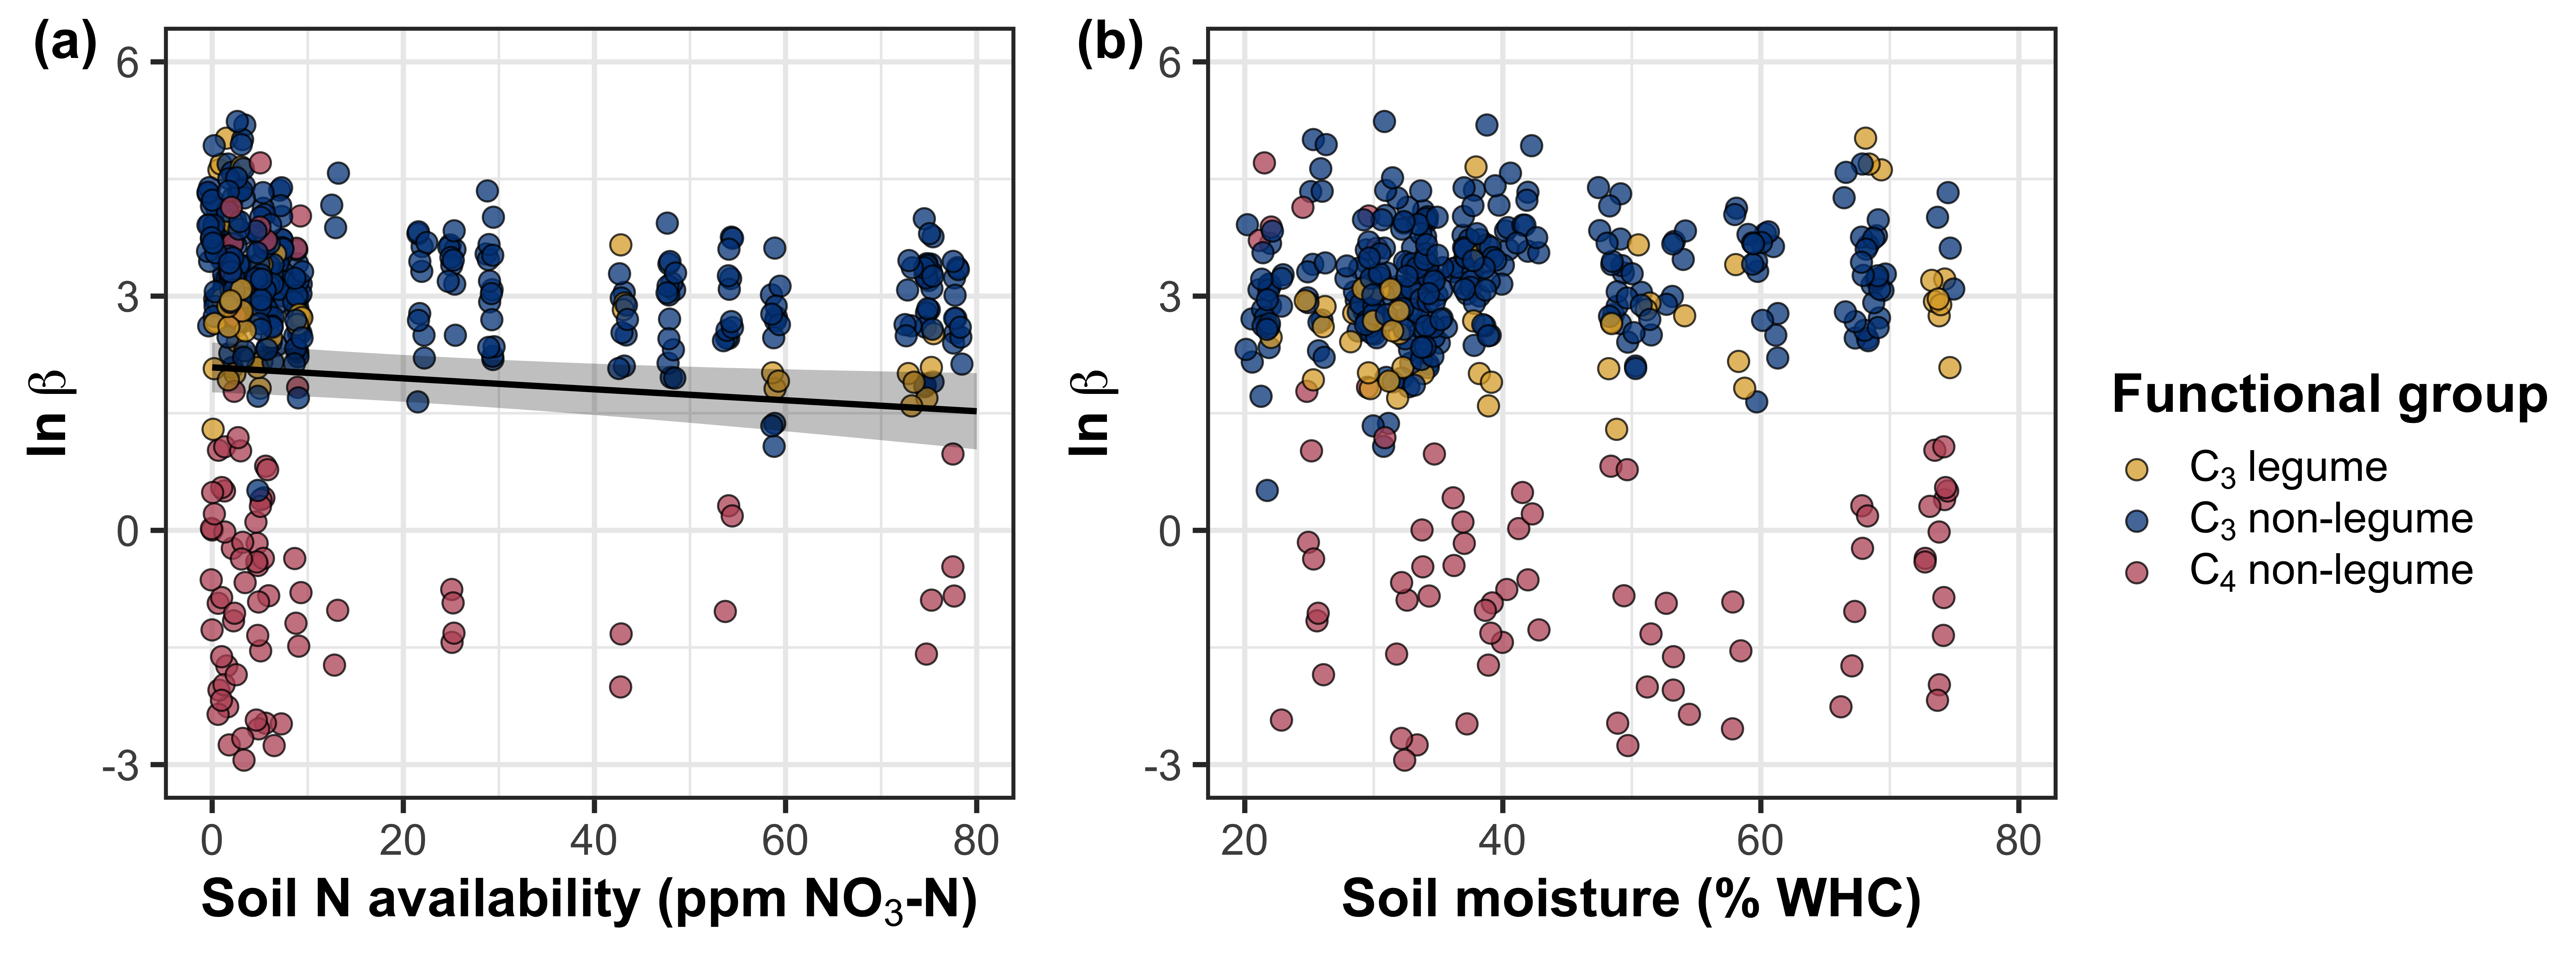
\includegraphics[scale = 0.075]{ch4_TXeco/figs/TXeco_fig2_beta.png}
    \caption[Effects of soil nitrogen availability and soil moisture on the unit cost ratio $\beta$]{Effects of soil nitrogen availability (a) and soil moisture (b) on the unit cost ratio $\beta$. In (b), soil moisture is represented as a percent of site water holding capacity. Yellow shading and trendlines indicate C$_3$ legumes, blue shading and trendlines indicate C$_3$ non-legumes, and red shading and trendlines indicate C$_4$ non-legumes. Points are jittered for visibility. Variably colored trendlines are only included if there is an interaction between the x-axis and plant functional group, where solid trendlines indicate slopes that are different from zero (\textit{p} < 0.05) and dashed trendlines indicate slopes that are not different from zero (\textit{p} < 0.05). Error ribbons represent the upper and lower 95\% confidence intervals of each fitted trendline.}
    \label{fig:figure4.2}
\end{figure}
\end{landscape}
\clearpage

\subsection{\textit{Leaf C\textsubscript{i}:C\textsubscript{a} ($\chi$)}}
Model selection indicated that 4-day daily VPD was the timescale that conferred the best model fit for $\chi$ (AICc = -883.97; Table S1; Fig. S2).

Variance in $\chi$ was driven by a series of two-way interactions between functional group and VPD (\textit{p} = 0.006; Table 3), soil moisture (\textit{p} = 0.033, Table \ref{fig:figure3.3}), and soil nitrogen availability (\textit{p} = 0.022; Table 3). The interaction between 4-day VPD and functional group revealed that the general negative effect of increasing VPD (\textit{p} < 0.001; Table 3) was driven by a negative effect of increasing VPD on $\chi$ in C$_3$ nonlegumes (Tukey: \textit{p} < 0.001) and marginal negative effect in C$_3$ legumes (Tukey: \textit{p} = 0.074) paired with a positive trending, but insignificant effect of increasing VPD in C$_4$ nonlegumes (Tukey: \textit{p} = 0.130; Fig. 3a). The interaction between 2-day soil moisture and functional group indicated that the general negative effect of increasing soil moisture on $\chi$ was driven by a positive effect of increasing soil moisture on $\chi$ in C$_4$ nonlegumes (Tukey: \textit{p} = 0.009) despite a positive trending but insignificant effect of increasing soil moisture on $\chi$ in C$_3$ legumes (Tukey: \textit{p} = 0.116) and a null effect of soil moisture on $\chi$ in C$_3$ nonlegumes (Tukey: \textit{p} = 0.693; Fig. 3c). The interaction between soil nitrogen availability and plant functional group revealed a weak negative effect of increasing soil nitrogen availability on $\chi$ in C$_3$ legumes (Tukey: \textit{p} = 0.045), with no apparent effect in C$_3$ nonlegumes (Tukey: \textit{p} = 0.706) or C$_4$ nonlegumes (Tukey: \textit{p} = 0.757). Finally, an individual effect of functional group (\textit{p} < 0.001; Table 3) revealed that C$_4$ nonlegumes generally had lower $\chi$ than C$_3$ legumes and C$_3$ nonlegumes (Tukey: \textit{p} < 0.001 in both cases), with no apparent difference between C$_3$ legumes and C$_3$ nonlegumes (Tukey: \textit{p} = 0.831).

\newpage
\begin{table}
    \centering
    \caption{Effects of soil moisture, soil nitrogen availability, and plant functional group on $\chi^*$}
    %\resizebox{\columnwidth}{!}{
        \begin{tabular}{p{6cm}p{0.5cm}p{2cm}p{1.5cm}p{1.5cm}}
            \hline 
            & \multicolumn{1}{r}{df} 
            & \multicolumn{1}{r}{Coefficient} 
            & \multicolumn{1}{r}{$\chi^{2}$} 
            & \multicolumn{1}{r}{\textit{p}} 
            \\ 
            \hline
            
            Intercept
            & \multicolumn{1}{r}{-}
            & \multicolumn{1}{r}{9.33E-01}
            & \multicolumn{1}{r}{-}
            & \multicolumn{1}{r}{-}
            \\

            Vapor pressure deficit (VPD\textsubscript{4})
            & \multicolumn{1}{r}{1}
            & \multicolumn{1}{r}{-1.78E-01}
            & \multicolumn{1}{r}{20.792}
            & \multicolumn{1}{r}{\textbf{<0.001}}
            \\

            Soil moisture (SM\textsubscript{2})
            & \multicolumn{1}{r}{1}
            & \multicolumn{1}{r}{4.53E-02}
            & \multicolumn{1}{r}{1.972}
            & \multicolumn{1}{r}{0.160}
            \\

            Soil N (N)
            & \multicolumn{1}{r}{1}
            & \multicolumn{1}{r}{-1.30E-03}
            & \multicolumn{1}{r}{0.168}
            & \multicolumn{1}{r}{0.682}
            \\

            PFT
            & \multicolumn{1}{r}{2}
            & \multicolumn{1}{r}{-}
            & \multicolumn{1}{r}{172.624}
            & \multicolumn{1}{r}{\textbf{<0.001}}
            \\

            SM\textsubscript{2}*N
            & \multicolumn{1}{r}{1}
            & \multicolumn{1}{r}{7.40E-04}
            & \multicolumn{1}{r}{0.849}
            & \multicolumn{1}{r}{0.357}
            \\

            VPD\textsubscript{4}*PFT
            & \multicolumn{1}{r}{2}
            & \multicolumn{1}{r}{-}
            & \multicolumn{1}{r}{10.241}
            & \multicolumn{1}{r}{\textbf{0.006}}
            \\

            SM\textsubscript{2}*PFT
            & \multicolumn{1}{r}{2}
            & \multicolumn{1}{r}{-}
            & \multicolumn{1}{r}{6.806}
            & \multicolumn{1}{r}{\textbf{0.033}}
            \\

            N*PFT
            & \multicolumn{1}{r}{2}
            & \multicolumn{1}{r}{-}
            & \multicolumn{1}{r}{7.602}
            & \multicolumn{1}{r}{\textbf{0.022}}
            \\

            SM\textsubscript{2}*N*PFT
            & \multicolumn{1}{r}{2}
            & \multicolumn{1}{r}{-}
            & \multicolumn{1}{r}{0.732}
            & \multicolumn{1}{r}{0.694}
            \\
            \hline
        \end{tabular}%}
    \label{tab:table4.3}
\end{table}
\noindent \textsuperscript{$*$}Significance determined using Type II Wald $\chi^{2}$ tests ($\alpha$ = 0.05). \textit{P}-values less than 0.05 are in bold and \textit{p}-values where 0.05 < \textit{p} < 0.1 are italicized. $\chi$ was not transformed prior to model fitting, so model coefficients are reported on the response scale. Model coefficients are only included for continuous fixed effects.
\clearpage

\newpage
\begin{figure}
    \centering
    
\includegraphics[scale = 0.07]{ch4_TXeco/figs/TXeco_fig3_chi.png}
    \caption[Effects of 4-day mean vapor pressure deficit, 2-day soil moisture (per water holding capacity), and soil nitrogen availability on $\chi$. ]{Effects of 4-day mean vapor pressure deficit (a), 2-day soil moisture (per water holding capacity; b), and soil nitrogen availability (c) on $\chi$. Shading and trendlines are as explained in Figure 2. Points are jittered for visibility. Variably colored trendlines are only included if there is an interaction between the x-axis and plant functional group, where solid trendlines indicate slopes that are different from zero (\textit{p} < 0.05) and dashed trendlines indicate slopes that are not different from zero (\textit{p} < 0.05). Error ribbons represent the upper and lower 95\% confidence intervals of each fitted trendline.}
    \label{fig:figure4.3}
\end{figure}
\clearpage

\subsection{\textit{Leaf nitrogen content}}
An interaction between $\chi$ and plant functional group (\textit{p} < 0.001; Table 4) revealed that the general negative effect of increasing $\chi$ on $N_\mathrm{area}$ (\textit{p} < 0.001; Table 4) was driven by a negative effect of increasing $\chi$ on $N_\mathrm{area}$ in C$_3$ nonlegumes (Tukey: \textit{p} < 0.001) and C$_3$ legumes (Tukey: \textit{p} = 0.002) despite a null effect of $\chi$ on $N_\mathrm{area}$ in C$_4$ nonlegumes (Tukey: \textit{p} = 0.795; Fig. 4a). An interaction between soil nitrogen availability and soil moisture (\textit{p} = 0.028; Table 4) indicated that the marginal positive effect of increasing soil nitrogen availability on $N_\mathrm{area}$ (\textit{p} = 0.091; Table 4) decreased with increasing soil moisture, despite no apparent individual effect of soil moisture on $N_\mathrm{area}$ (\textit{p} = 0.692; Table 4). Finally, a plant functional group effect (\textit{p} < 0.001; Table 4) indicated that C$_4$ nonlegumes had lower $N_\mathrm{area}$ values on average compared to C$_3$ legumes (Tukey: \textit{p} < 0.001) and C$_3$ nonlegumes (Tukey: \textit{p} = 0.001), while C$_3$ legumes had lower average $N_\mathrm{area}$ values compared to C$_3$ nonlegumes (Tukey: \textit{p} = 0.012).

A marginal interaction between $\chi$ and plant functional group (\textit{p} = 0.088; Table 4) revealed that, despite no apparent general effect of $\chi$ on $N_\mathrm{mass}$ (\textit{p} = 0.273; Table 4), increasing $\chi$ decreased $N_\mathrm{mass}$ in C$_3$ nonlegumes (Tukey: \textit{p} = 0.021), but this effect was not apparent in C$_4$ nonlegumes (Tukey: \textit{p} = 0.693) or C$_3$ legumes (Tukey: p = 0.477). An interaction between soil nitrogen availability and soil moisture (\textit{p} < 0.001; Table 4) indicated that the general positive effect of increasing soil nitrogen availability on $N_\mathrm{mass}$ (\textit{p} < 0.001; Table 4) generally decreased with increasing soil moisture, despite an apparent general positive effect of increasing soil moisture on $N_\mathrm{mass}$ (\textit{p} < 0.001; Table 4). This interaction indicated that the positive effect of increasing soil nitrogen availability on $N_\mathrm{mass}$ was only apparent when soil moisture was less than 70\% the maximum water holding capacity (Tukey: \textit{p} < 0.05 in all cases) despite a positive effect of increasing soil moisture on $N_\mathrm{mass}$ (\textit{p} < 0.001; Table 4). Finally, a plant functional group effect (\textit{p} < 0.001; Table 4) indicated that C$_4$ nonlegumes had lower $N_\mathrm{mass}$ values on average compared to C$_3$ legumes (Tukey: \textit{p} = 0.002) and C$_3$ nonlegumes (Tukey: \textit{p} = 0.019), while $N_\mathrm{mass}$ did not differ between C$_3$ legumes and C$_3$ nonlegumes (Tukey: p = 0.149).

An interaction between $\chi$ and functional group (\textit{p} = 0.005; Table 4) indicated that the general negative effect of increasing $\chi$ on $M_\mathrm{area}$ (\textit{p} < 0.001; Table 4; Fig. 4c) was driven by a negative effect of increasing $\chi$ on $M_\mathrm{area}$ in C$_3$ legumes and C$_3$ nonlegumes (Tukey: \textit{p} < 0.001 in both cases) despite a nonsignificant effect of increasing $\chi$ on $M_\mathrm{area}$ in C$_4$ nonlegumes (Tukey: \textit{p} = 0.724). An interaction between soil nitrogen and soil moisture (\textit{p} < 0.001; Table 4) indicated that the general negative effect of increasing soil nitrogen availability on $M_\mathrm{area}$ (\textit{p} < 0.001; Table 4) decreased with increasing soil moisture, despite an apparent general negative effect of increasing soil moisture on $M_\mathrm{area}$ (\textit{p} = 0.002; Table 4). Specifically, the negative effect of increasing soil nitrogen availability on $M_\mathrm{area}$ was only apparent when soil moisture was less than 65\% the maximum water holding capacity (Tukey: \textit{p} < 0.05 in all cases). An additional interaction between soil nitrogen availability and functional group (\textit{p} = 0.034; Table 4) indicated that the general negative effect of increasing soil nitrogen availability on $M_\mathrm{area}$ was driven by decreases in C$_3$ nonlegumes (Tukey: \textit{p} < 0.001) and C$_4$ nonlegumes (Tukey: \textit{p} = 0.003), with no apparent effect of soil nitrogen availability on $M_\mathrm{area}$ in C$_3$ legumes (Tukey: \textit{p} = 0.997).

\newpage
\begin{landscape}
    \begin{table}
    \centering
    \caption{Effects of soil nitrogen fertilization, inoculation, and CO$_2$ treatments on $N_\mathrm{area}$, $N_\mathrm{mass}$, and $M_\mathrm{area}$}
    \resizebox{\columnwidth}{!}{
        \begin{tabular}{p{3.75cm}p{0.5cm}p{1.75cm}p{1.5cm}p{1.5cm}p{1.75cm}p{1.5cm}p{1.5cm}p{1.75cm}p{1.5cm}p{1.5cm}}
            && 
            \multicolumn{3}{l}{$N_\mathrm{area}$} 
            & \multicolumn{3}{l}{$N_\mathrm{mass}$} 
            & \multicolumn{3}{l}{$M_\mathrm{area}$} 
            \\
            \hline 
            & 
            \multicolumn{1}{r}{df} 
            & \multicolumn{1}{r}{Coefficient}   & \multicolumn{1}{r}{$\chi^{2}$}    & \multicolumn{1}{r}{\textit{p}} 
            & \multicolumn{1}{r}{Coefficient}   & \multicolumn{1}{r}{$\chi^{2}$}    & \multicolumn{1}{r}{\textit{p}} 
            & \multicolumn{1}{r}{Coefficient}   & \multicolumn{1}{r}{$\chi^{2}$}    & \multicolumn{1}{r}{\textit{p}} 
            \\ 
            \hline

            (Intercept) & \multicolumn{1}{r}{-} 
            &  \multicolumn{1}{r}{2.78E+00}     & \multicolumn{1}{r}{-}             & \multicolumn{1}{r}{-}
            &  \multicolumn{1}{r}{4.42E-01}     & \multicolumn{1}{r}{-}             & \multicolumn{1}{r}{-}
            &  \multicolumn{1}{r}{6.97E+00}     & \multicolumn{1}{r}{-}             & \multicolumn{1}{r}{-} 
            \\

            $\chi$ & \multicolumn{1}{r}{1}
            & \multicolumn{1}{r}{-2.53E+00}     & \multicolumn{1}{r}{15.771}        & \multicolumn{1}{r}{\textbf{<0.001}}
            & \multicolumn{1}{r}{4.56E-01}      & \multicolumn{1}{r}{1.201}         & \multicolumn{1}{r}{0.273}
            & \multicolumn{1}{r}{-3.10E+00}     & \multicolumn{1}{r}{20.620}        & \multicolumn{1}{r}{\textbf{<0.001}} 
            \\


            Soil N (N) & \multicolumn{1}{r}{1}
            & \multicolumn{1}{r}{1.08E-02}      & \multicolumn{1}{r}{2.855}         & \multicolumn{1}{r}{\textit{0.091}}
            & \multicolumn{1}{r}{1.37E-02}      & \multicolumn{1}{r}{54.531}        & \multicolumn{1}{r}{\textbf{<0.001}}
            & \multicolumn{1}{r}{-2.87E-03}     & \multicolumn{1}{r}{29.759}        & \multicolumn{1}{r}{\textbf{<0.001}} 
            \\

            Soil moisture (SM\textsubscript{2}) & \multicolumn{1}{r}{1}
            & \multicolumn{1}{r}{3.61E-01}      & \multicolumn{1}{r}{0.157}         & \multicolumn{1}{r}{0.692}
            & \multicolumn{1}{r}{5.04E-01}      & \multicolumn{1}{r}{16.255}        & \multicolumn{1}{r}{\textbf{<0.001}}
            & \multicolumn{1}{r}{-1.26E-01}     & \multicolumn{1}{r}{9.282}         & \multicolumn{1}{r}{\textbf{ 0.002}} 
            \\

            PFT & \multicolumn{1}{r}{1}
            & \multicolumn{1}{r}{-}             & \multicolumn{1}{r}{60.641}        & \multicolumn{1}{r}{\textbf{<0.001}}
            & \multicolumn{1}{r}{-}             & \multicolumn{1}{r}{21.539}        & \multicolumn{1}{r}{\textbf{<0.001}}
            & \multicolumn{1}{r}{-}             & \multicolumn{1}{r}{11.520}        & \multicolumn{1}{r}{\textbf{0.003}} 
            \\

            SM\textsubscript{2}*N & \multicolumn{1}{r}{1}
            & \multicolumn{1}{r}{-1.09E-02}     & \multicolumn{1}{r}{4.779}         & \multicolumn{1}{r}{\textbf{ 0.029}}
            & \multicolumn{1}{r}{-1.76E-02}     & \multicolumn{1}{r}{41.784}        & \multicolumn{1}{r}{\textbf{<0.001}}
            & \multicolumn{1}{r}{6.35E-03}      & \multicolumn{1}{r}{14.111}        & \multicolumn{1}{r}{\textbf{<0.001}} 
            \\

            $\chi$*PFT & \multicolumn{1}{r}{1}
            & \multicolumn{1}{r}{-}             & \multicolumn{1}{r}{15.188}        & \multicolumn{1}{r}{\textbf{<0.001}}
            & \multicolumn{1}{r}{-}             & \multicolumn{1}{r}{4.864}         & \multicolumn{1}{r}{\textit{ 0.088}}
            & \multicolumn{1}{r}{-}             & \multicolumn{1}{r}{17.032}        & \multicolumn{1}{r}{\textbf{ 0.025}} 
            \\

            N*PFT & \multicolumn{1}{r}{1}
            & \multicolumn{1}{r}{-}             & \multicolumn{1}{r}{2.289}         & \multicolumn{1}{r}{0.318}
            & \multicolumn{1}{r}{-}             & \multicolumn{1}{r}{0.914}         & \multicolumn{1}{r}{0.633}
            & \multicolumn{1}{r}{-}             & \multicolumn{1}{r}{6.760}         & \multicolumn{1}{r}{\textbf{0.034}}
            \\

            SM\textsubscript{2}*PFT & \multicolumn{1}{r}{1}
            & \multicolumn{1}{r}{-}             & \multicolumn{1}{r}{0.978}         & \multicolumn{1}{r}{0.613}
            & \multicolumn{1}{r}{-}             & \multicolumn{1}{r}{0.128}         & \multicolumn{1}{r}{0.938}
            & \multicolumn{1}{r}{-}             & \multicolumn{1}{r}{2.121}         & \multicolumn{1}{r}{0.346} 
            \\

            SM\textsubscript{2}*N*PFT & \multicolumn{1}{r}{1}
            & \multicolumn{1}{r}{-}             & \multicolumn{1}{r}{1.289}         & \multicolumn{1}{r}{0.525}
            & \multicolumn{1}{r}{-}             & \multicolumn{1}{r}{2.180}         & \multicolumn{1}{r}{0.336}
            & \multicolumn{1}{r}{-}             & \multicolumn{1}{r}{0.629}         & \multicolumn{1}{r}{0.730}
            \\
            \hline

    \end{tabular}}
    \label{tab:table4.4}
    \end{table}
    \noindent \textsuperscript{$*$}Significance determined using Type II Wald $\chi^{2}$ tests ($\alpha$ = 0.05). \textit{P}-values less than 0.05 are in bold and \textit{p}-values where 0.05 < \textit{p} < 0.1 are italicized. Coefficients are reported on the natural-log scale and are only included for continuous fixed effects.
\end{landscape}
\clearpage

\newpage
    \begin{figure}
        \centering
        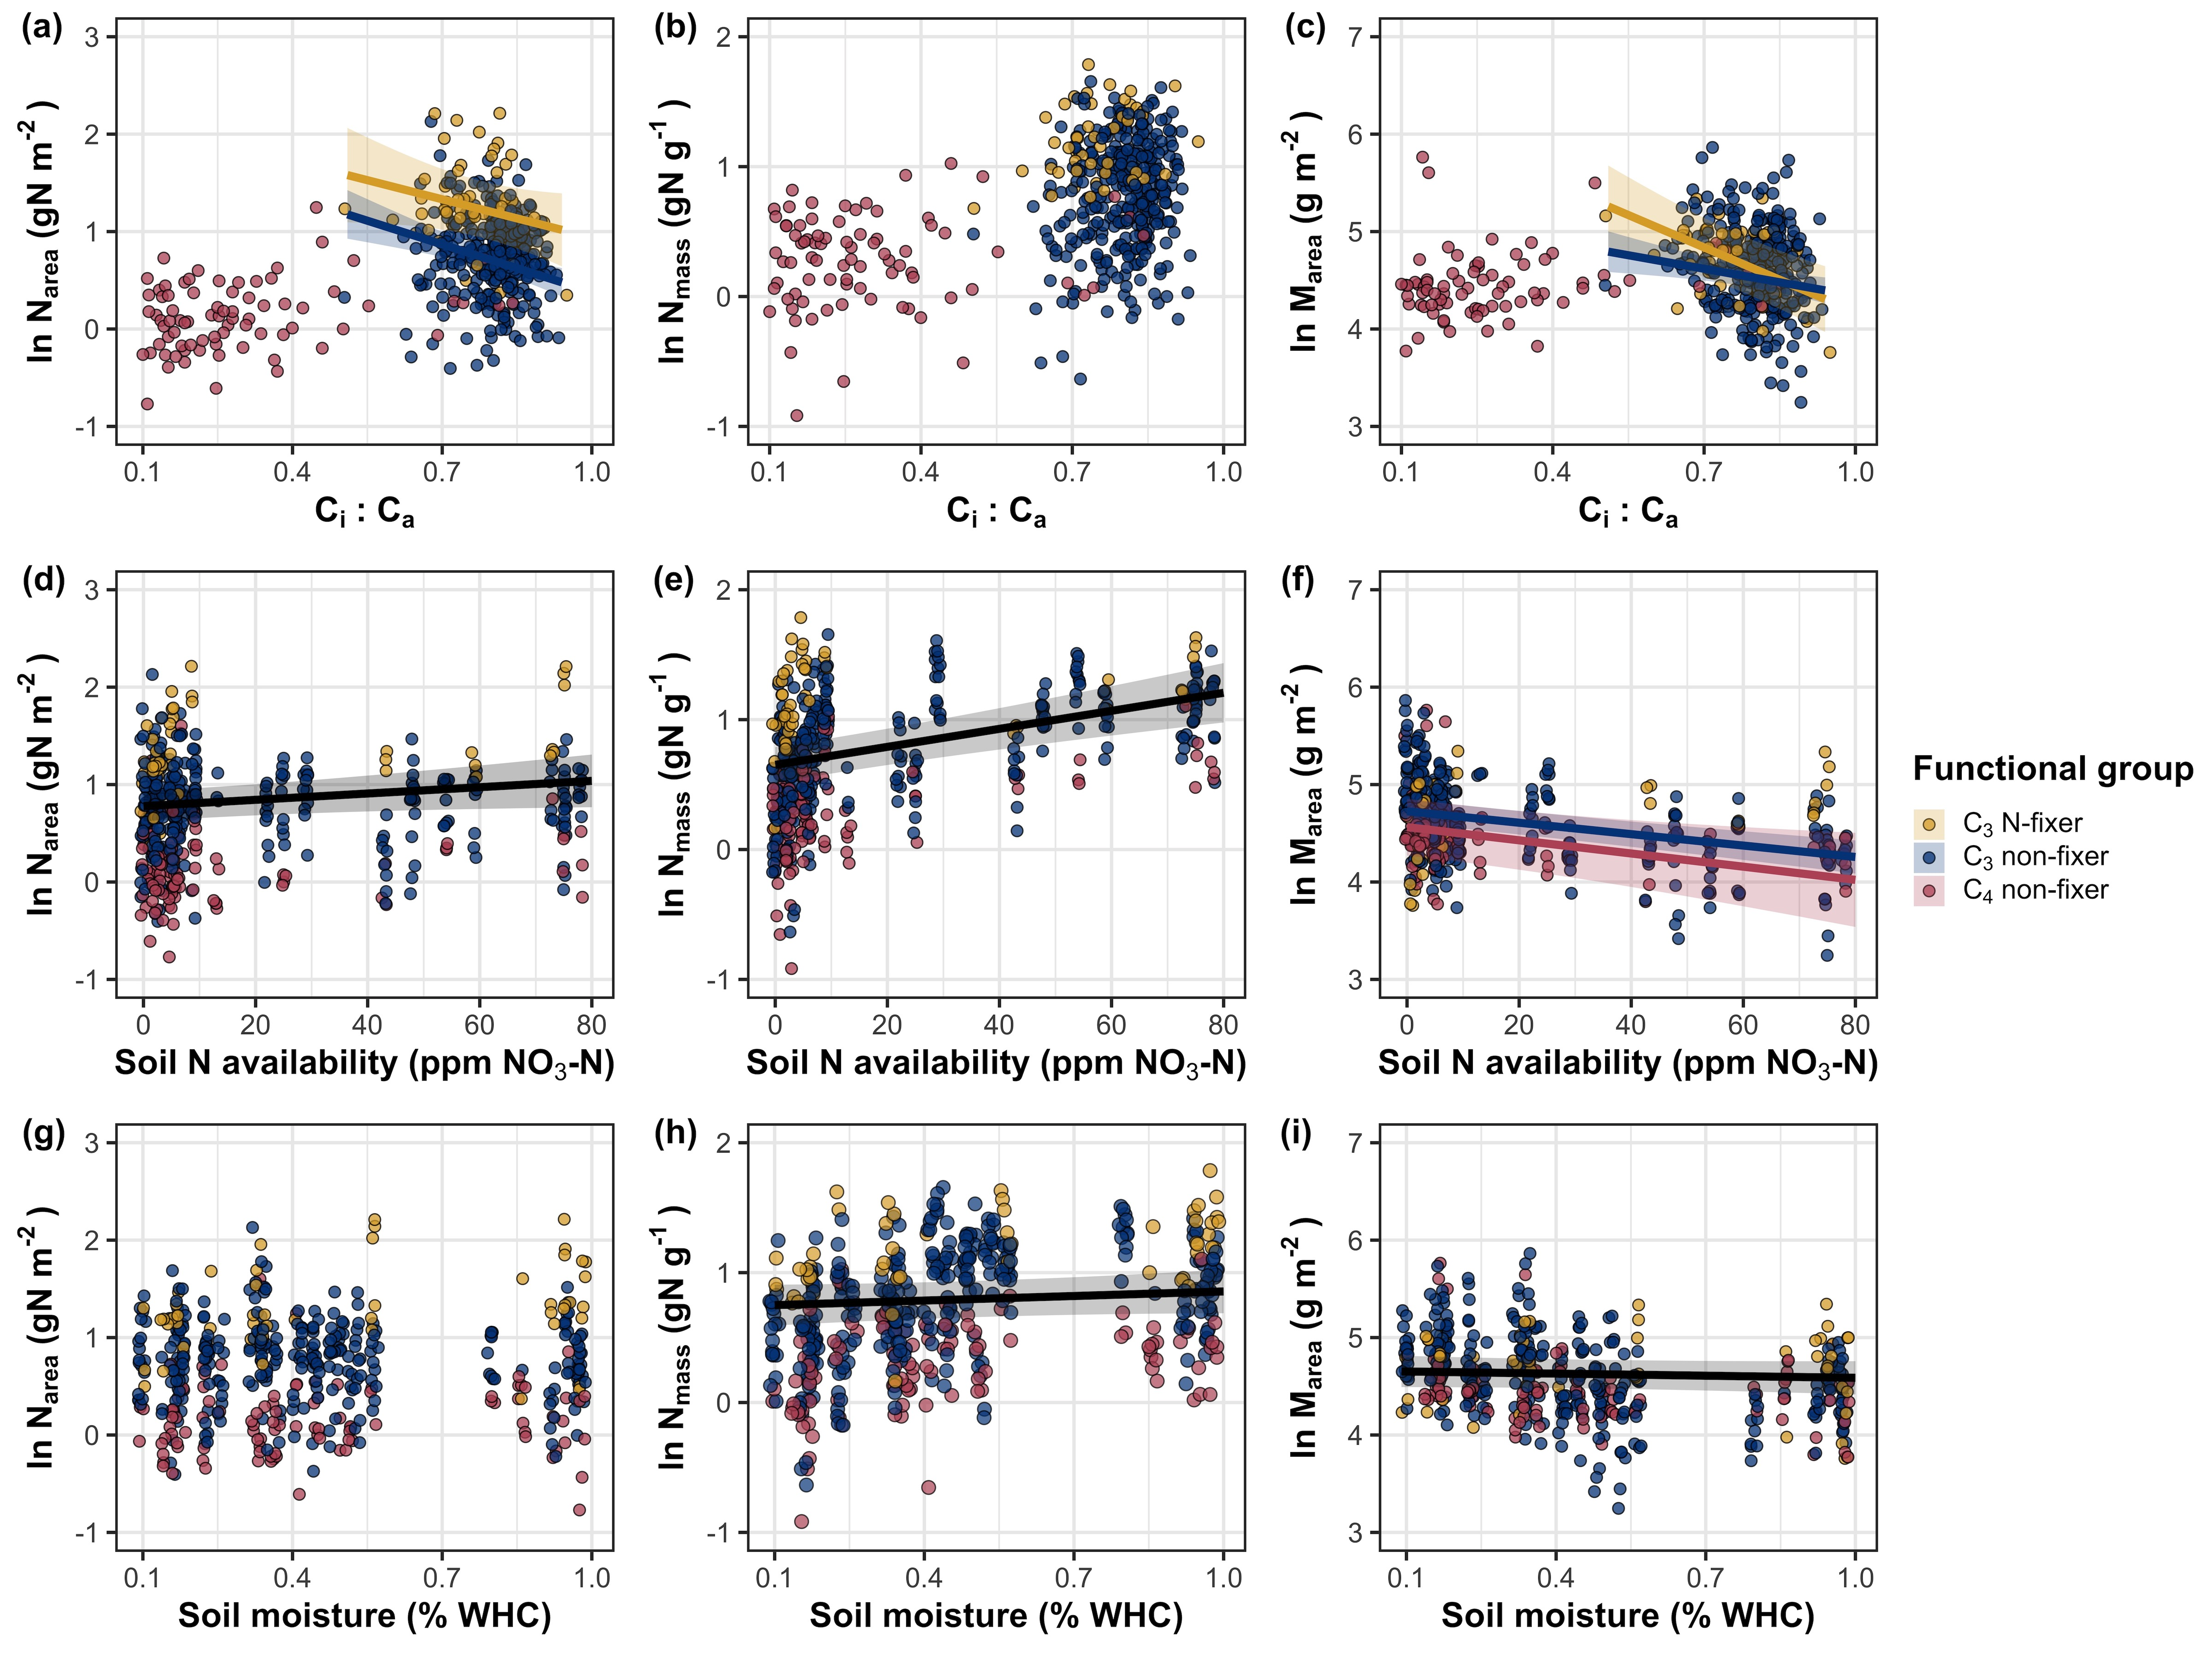
\includegraphics[scale = 0.042]{ch4_TXeco/figs/TXeco_fig4_narea.png}
        \caption[Effects of $\chi$, soil nitrogen availability, and soil moisture on leaf nitrogen content per unit leaf area, leaf nitrogen content per unit leaf biomass, and leaf mass per area.]{Effects of $\chi$ (a-c), soil nitrogen availability (d-f), and soil moisture (g-i) on leaf nitrogen content per unit leaf area (a, d, g), leaf nitrogen content per unit leaf biomass (b, e, h), and leaf mass per area (c, f, i). A solid black trendline indicates the bivariate relationship between the fixed effect the x-axis and response variable on the y-axis and is only included when there is no interaction between the x-axis and plant functional group.}
        \label{fig:figure4.4}
    \end{figure}
\clearpage

\subsection{\textit{Structural equation model}}
The piecewise structural equation model explained 90\%, 54\%, 80\%, 92\%, and 41\% of variance in $N_\mathrm{area}$, $N_\mathrm{mass}$, $M_\mathrm{area}$, $\chi$, and $\beta$, respectively (Table 5; Fig. 5). Variance in $N_\mathrm{area}$ was driven by a negative effect of increasing $\chi$ (\textit{p} < 0.001; Table 5) paired with positive effects of increasing $N_\mathrm{mass}$ and $M_\mathrm{area}$ (\textit{p} < 0.001 in both cases; Table 5; Fig. 5). Model results indicated that the negative effect of $\chi$ on $N_\mathrm{area}$ was driven by a strong reduction in $M_\mathrm{area}$ with increasing $\chi$ (\textit{p} < 0.001; Table 5) paired with no change in $\chi$ due to $N_\mathrm{mass}$ (\textit{p} = 0.150; Table 5). However, there was a strong negative effect of increasing $M_\mathrm{area}$ on $N_\mathrm{mass}$ (\textit{p} < 0.001; Table 5; Fig. 5). $\chi$ generally increased with increasing $\beta$  (\textit{p} < 0.001; Table 5) and decreased with increasing VPD (\textit{p} < 0.001; Table 5; Fig. 5). Variance in $\beta$  was driven by a negative effect of increasing soil nitrogen availability (\textit{p} < 0.001; Table 5) and was generally higher in C$_3$ species (\textit{p} < 0.001; Table 5; Fig. 5). However, $\beta$ did not change with soil moisture (\textit{p} = 0.332; Table 5) or with ability to acquire nitrogen via symbiotic nitrogen fixation (\textit{p} = 0.546; Table 5). Finally, soil nitrogen availability was positively associated with increasing soil moisture (\textit{p} < 0.001; Table 5; Fig. 5), while VPD was negatively associated with increasing soil moisture (\textit{p} < 0.001; Table 5; Fig. 5).

\newpage
\begin{table}
    \centering
    \caption{Structural equation model results investigating direct effects of climatic and soil resource availability on $N_\mathrm{area}$, $N_\mathrm{mass}$, $M_\mathrm{area}$, $\chi$, and $\beta$}
    %\resizebox{\columnwidth}{!}{
        \begin{tabular}{p{0.5cm}p{3cm}p{1.5cm}p{1.5cm}}
            \hline
            & Predictor & \multicolumn{1}{r}{Coefficient} & \multicolumn{1}{r}{\textit{p}} \\
            \hline

            \multicolumn{2}{l}{$N_\mathrm{area}$ ($R^2{}_c$) = 0.90} && \\
            & \multicolumn{1}{l}{$\chi$} & \multicolumn{1}{r}{-0.140} & \multicolumn{1}{r}{\textbf{<0.001}} \\
            & \multicolumn{1}{l}{$M_\mathrm{area}$} & \multicolumn{1}{r}{0.807} & \multicolumn{1}{r}{\textbf{<0.001}} \\
            & \multicolumn{1}{l}{$N_\mathrm{mass}$} & \multicolumn{1}{r}{0.795} & \multicolumn{1}{r}{\textbf{<0.001}} \\
            \hline

            \multicolumn{2}{l}{$N_\mathrm{mass}$ ($R^2{}_c$) = 0.54} && \\
            & \multicolumn{1}{l}{$\chi$} & \multicolumn{1}{r}{0.097} & \multicolumn{1}{r}{\textbf{<0.001}} \\
            \hline

            \multicolumn{2}{l}{$M_\mathrm{area}$ ($R^2{}_c$) = 0.80} && \\
            & \multicolumn{1}{l}{$\chi$} & \multicolumn{1}{r}{-0.372} & \multicolumn{1}{r}{0.150} \\
            & \multicolumn{1}{l}{$M_\mathrm{area}$} & \multicolumn{1}{r}{-0.303} & \multicolumn{1}{r}{\textbf{<0.001}} \\
            \hline

            \multicolumn{2}{l}{$\chi$ ($R^2{}_c$) = 0.92} && \\
            & \multicolumn{1}{l}{$\beta$} & \multicolumn{1}{r}{0.261} & \multicolumn{1}{r}{\textbf{<0.001}} \\
            & \multicolumn{1}{l}{VPD\textsubscript{4}} & \multicolumn{1}{r}{-0.122} & \multicolumn{1}{r}{\textbf{<0.001}} \\
            \hline

            \multicolumn{2}{l}{$\beta$ ($R^2{}_c$) = 0.41} && \\
            & \multicolumn{1}{l}{Soil N} & \multicolumn{1}{r}{-0.201} & \multicolumn{1}{r}{\textbf{<0.001}} \\
            & \multicolumn{1}{l}{SM\textsubscript{2}} & \multicolumn{1}{r}{-0.048} & \multicolumn{1}{r}{0.332} \\
            & \multicolumn{1}{l}{Photo. pathway} & \multicolumn{1}{r}{0.490} & \multicolumn{1}{r}{\textbf{<0.001}} \\
            & \multicolumn{1}{l}{N-fixing ability} & \multicolumn{1}{r}{-0.053} & \multicolumn{1}{r}{0.546} \\
            \hline

            \multicolumn{2}{l}{Soil N ($R^2{}_c$) = 0.39} && \\
            & \multicolumn{1}{l}{SM\textsubscript{2}} & \multicolumn{1}{r}{0.410} & \multicolumn{1}{r}{\textbf{<0.001}} \\
            \hline

        \end{tabular}%}
        \label{tab:table4.5}
    \end{table}
\begin{singlespace}
    \noindent \textsuperscript{$*$}Reported coefficients are standardized across the structural equation model. \textit{P}-values less than 0.05 are noted in bold. Positive coefficients for photosynthetic pathway indicate generally larger values in C\textsubscript{3} species, while positive coefficients for N-fixing ability indicate generally larger values in N-fixing species. Key: $N_\mathrm{area}$=leaf nitrogen content per unit leaf area, $M_\mathrm{area}$=leaf mass per unit leaf dry biomass, $N_\mathrm{mass}$=leaf nitrogen content per unit leaf dry biomass, $\beta$=cost of acquiring nitrogen relative to water, $\chi$=isotope-derived estimate of the leaf Ci:Ca ratio, VPD\textsubscript{4}= 4-day mean vapor pressure deficit, SM\textsubscript{2}=2-day mean soil moisture, R\textsuperscript{2}\textsubscript{c} = conditional R\textsuperscript{2} value
\end{singlespace}
\clearpage

\newpage
\begin{landscape}
    \begin{figure}
        \centering
        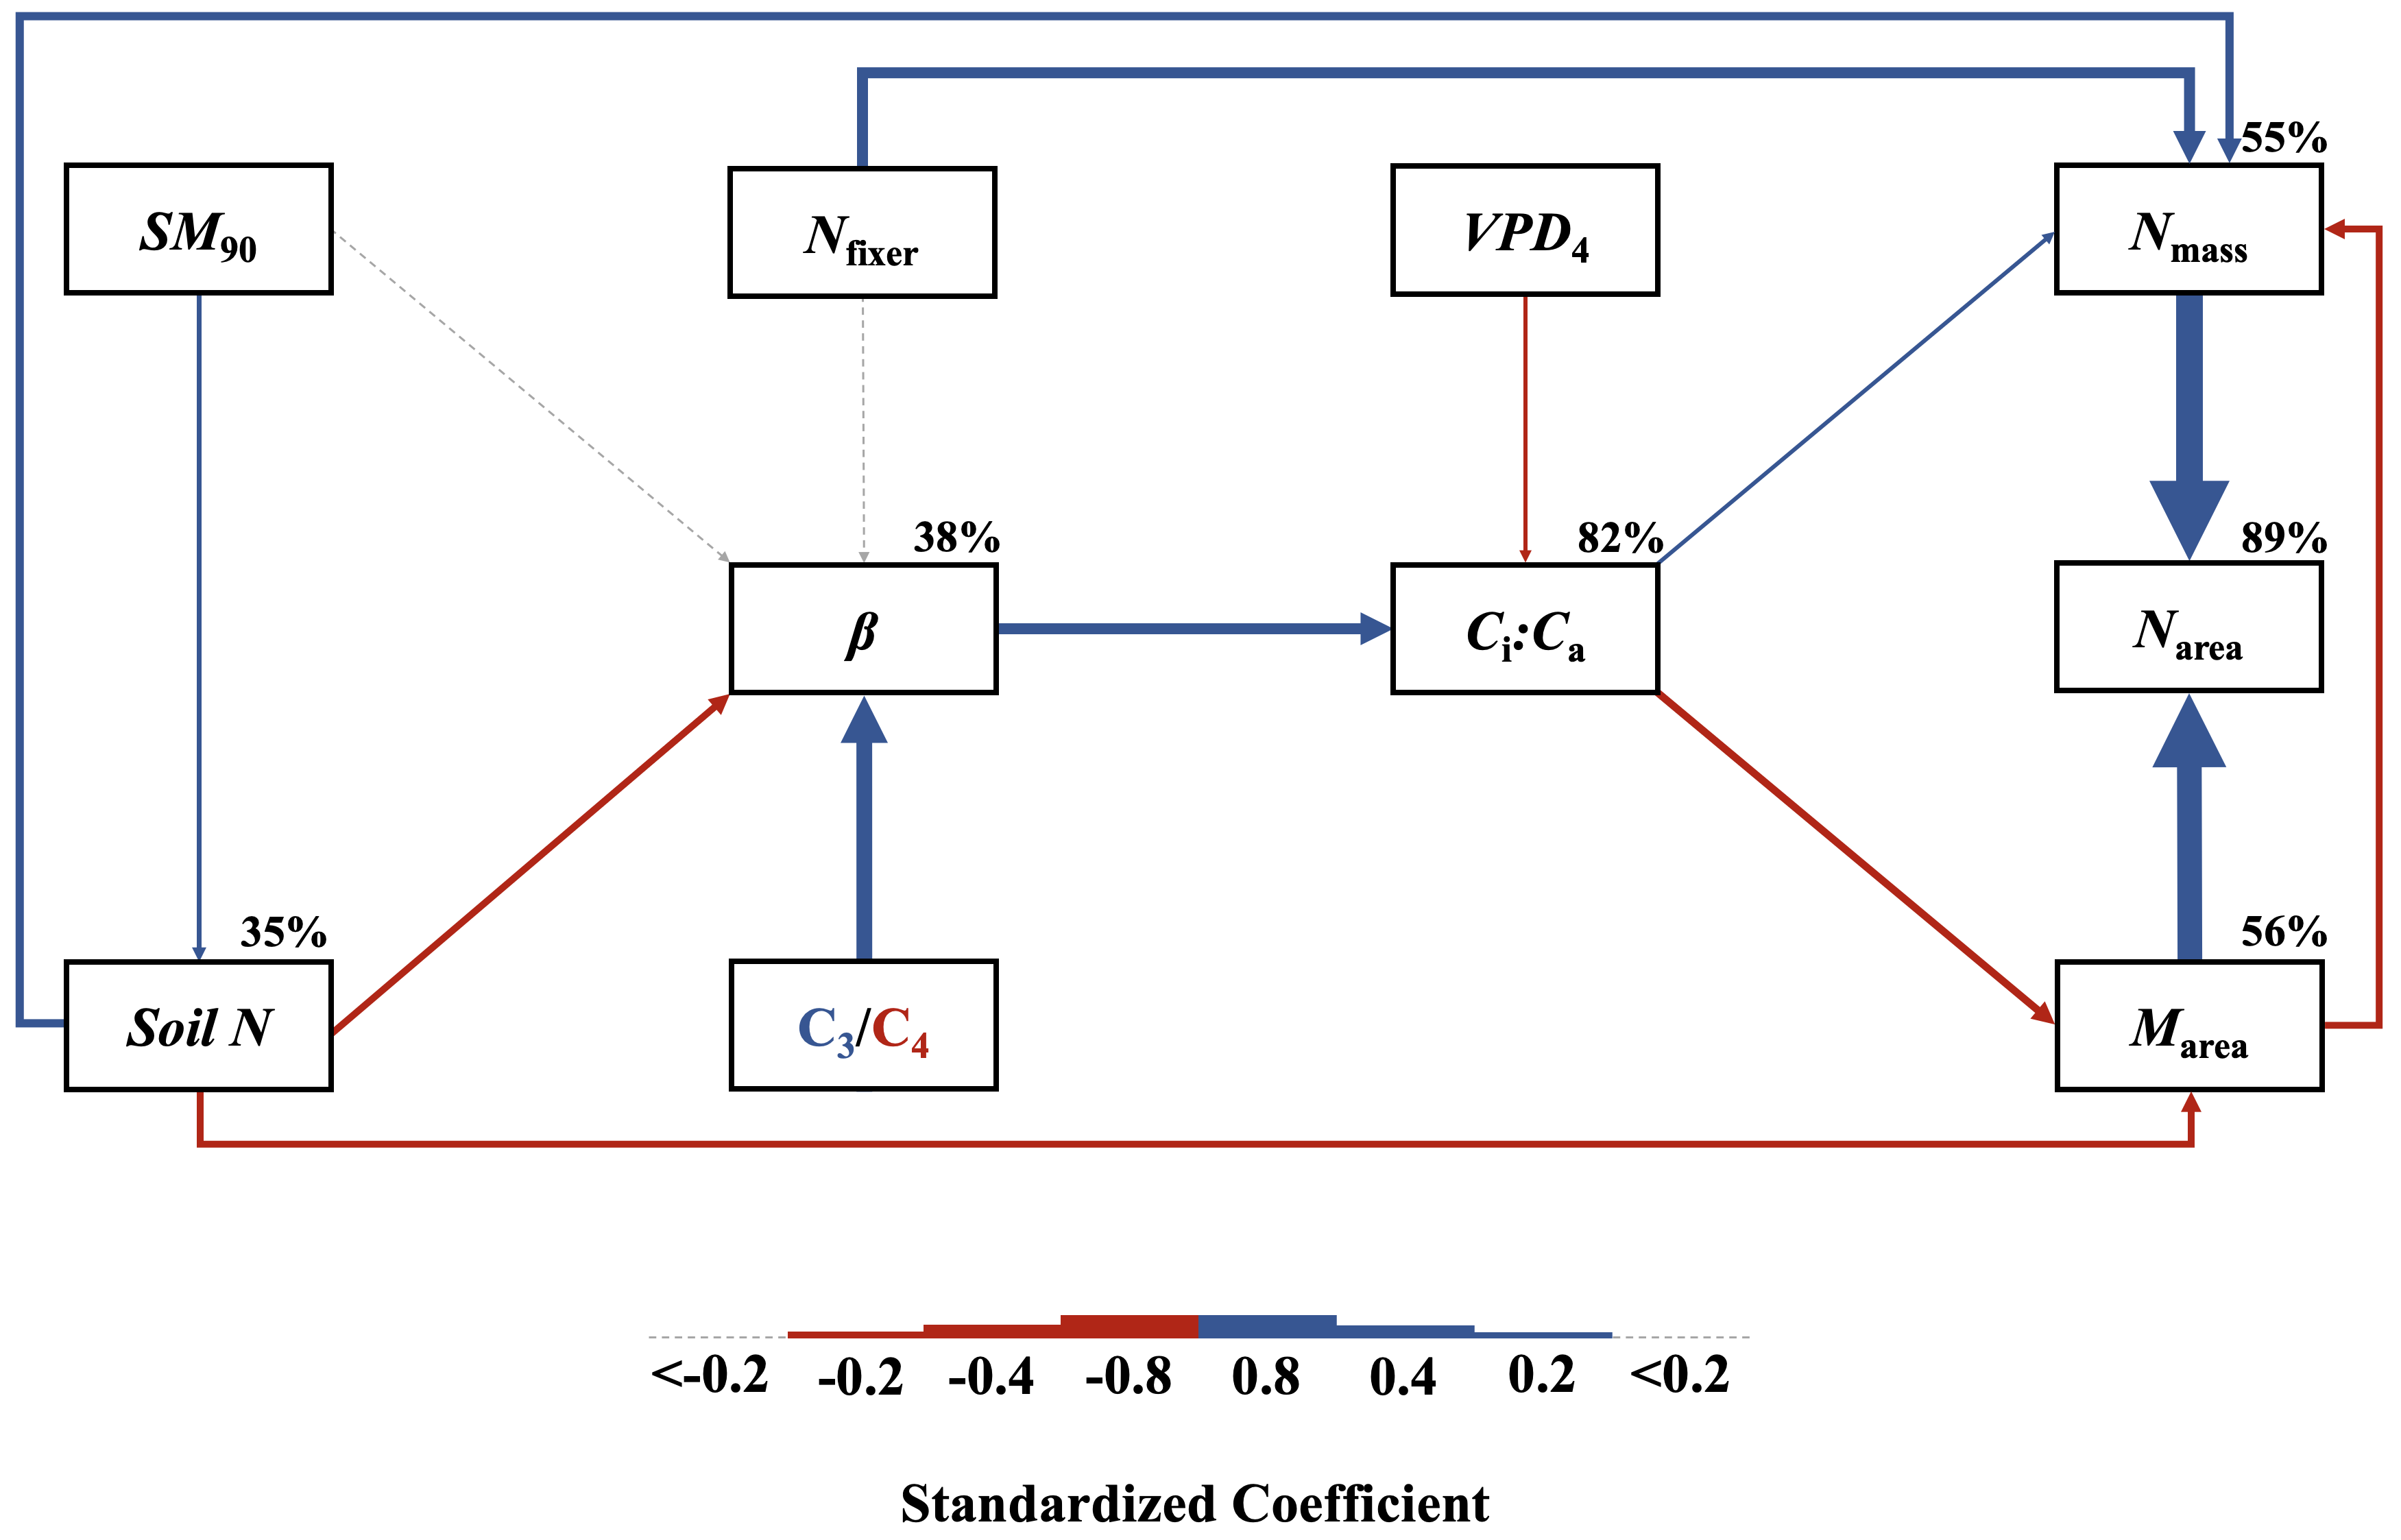
\includegraphics[scale = 0.3]{ch4_TXeco/figs/TXeco_fig5_SEM.png}
        \caption[Structural equation model results exploring direct and indirect drivers of $N_\mathrm{area}$]{Structural equation model results exploring direct and indirect drivers of $N_\mathrm{area}$. Boxes indicate measured edaphic factors, climatic factors, and leaf traits. Percentages above boxes indicate conditional $R^{2}$ values of each respective leaf trait. Solid arrows indicate bivariate relationships where \textit{p} < 0.05, while dashed arrows indicate bivariate relationships where \textit{p} > 0.05. Positive model coefficients are indicated through blue arrows, while negative model coefficients are indicated through red arrows. Arrow thickness scales with the standardized model coefficient of each bivariate relationship. A positive coefficient for photosynthetic pathway indicates generally larger values in C$_3$ species, while a positive coefficient for $N_\mathrm{fixer}$ indicates generally larger values in N-fixing species. Standardized model coefficients and associated \textit{p}-values are reported in Table 5.}
        \label{fig:figure4.5}
    \end{figure}
\end{landscape}
\clearpage


\section{Discussion}
In this study, we quantified direct and indirect effects of soil resource availability, climate, $\chi$, and $\beta$ on $N_\mathrm{area}$ and components of $N_\mathrm{area}$ ($N_\mathrm{mass}$ and $M_\mathrm{area}$) in 520 individuals spanning across a soil resource availability and climate gradient in Texas, USA. We found consistent support for patterns expected from photosynthetic least-cost theory, a result driven by a strong direct negative relationship between the relative costs to acquire nitrogen versus water ($\beta$) on $N_\mathrm{area}$ as mediated through changes in the leaf C\textsubscript{i}:C\textsubscript{a} ratio ($\chi$). In further support of patterns expected from theory, increasing soil nitrogen availability had a strong negative effect on $\beta$, resulting in an indirect stimulation in $N_\mathrm{area}$. Increasing VPD also indirectly increased $N_\mathrm{area}$ through a direct negative effect of increasing VPD on $\chi$. Interestingly, we found a strong positive association between soil moisture and soil nitrogen availability resulted in an indirect positive effect of increasing soil moisture on $N_\mathrm{area}$ despite an apparent null direct effect of soil moisture on $N_\mathrm{area}$. Overall, results provide strong and consistent support for patterns expected from photosynthetic least-cost theory, showing that both soil resource availability and climate drive variance in $N_\mathrm{area}$ through changes in $\chi$.

\subsection{\textit{Negative effects of $\chi$ on $N_\mathrm{area}$ are driven by reductions in $M_\mathrm{area}$, not $N_\mathrm{mass}$}}
A strong negative effect of increasing $\chi$ on $N_\mathrm{area}$ was detected in both the linear mixed effect and piecewise structural equation models. The negative response of $N_\mathrm{area}$ to increasing $\chi$ is consistent with previous environmental gradient \shortcite{Dong2017,Querejeta2022} and manipulation experiments (Perkowski et al. n.d.), showing strong support for the nitrogen-water use tradeoffs expected from photosynthetic least cost theory \shortcite{Wright2003,Prentice2014}. Negative effects of increasing $\chi$ on $N_\mathrm{area}$ were driven by a strong negative effect of increasing $\chi$ on $M_\mathrm{area}$, with no apparent effect of $\chi$ on $N_\mathrm{mass}$, suggesting that changes in $N_\mathrm{area}$ were driven by changes in leaf structure and not leaf chemistry. Interestingly, increasing $M_\mathrm{area}$ was negatively associated with $N_\mathrm{mass}$, indicating that an increase in $N_\mathrm{mass}$ was associated with larger, thinner leaves (i.e. lower $M_\mathrm{area}$). These results are consistent with patterns reported from previous studies indicating that variance in $N_\mathrm{area}$ is driven by changes in $M_\mathrm{area}$ across environmental gradients, and that part of this response is due to negative covariance between $M_\mathrm{area}$ and $N_\mathrm{mass}$ associated with tradeoffs between leaf longevity and leaf productivity \shortcite{Wright2004,Dong2017,Dong2022a,Wang2023,Querejeta2022}.

The negative relationship between $\chi$ and $M_\mathrm{area}$ could be also response that allows leaves to maximize productivity in shorter-lived leaves. Tradeoffs between leaf longevity and leaf productivity are commonly observed and are included in a continuum of coordinated leaf traits that position individuals along a fast- or slow-growing leaf economics spectrum \shortcite{Wright2004,Onoda2004,Onoda2017,Reich2014,Wang2023}. Negative relationships between $\chi$ and $M_\mathrm{area}$ indicate that increased stomatal conductance and reduced water use efficiency were associated with thinner, larger leaves (i.e., lower $M_\mathrm{area}$). These patterns, combined with the negative relationship between $M_\mathrm{area}$ and $N_\mathrm{mass}$ mentioned above, likely allowed individuals to maximize light interception and productivity by exploiting high light environments, though this may come at the expense of increased water loss and decreased water-use efficiency. This strategy may be especially advantageous for fast-growing species in open canopy systems. In this study, C$_3$ legumes and C$_3$ nonlegumes dominated the dataset (78\% of total sampling effort), of which 22\% (17\% of total sampling effort) were classified as annual species with short growing seasons. We observed no effect of $\chi$ on $N_\mathrm{area}$ or $M_\mathrm{area}$ in C$_4$ nonlegumes, which made up 22\% of the sampling effort and were generally classified as warm season graminoid species with slower growth rates and longer growing seasons. These patterns indicate that stronger tradeoffs between nitrogen and water use may be more apparent in fast-growing species with high demand for building and maintaining productive leaf tissues.

\subsection{\textit{Soil nitrogen availability increases $N_\mathrm{area}$ through changes in the cost to acquire nitrogen}}
The null effect of soil nitrogen availability on $N_\mathrm{area}$ was driven by positive and negative respective effects of increasing soil nitrogen availability on $N_\mathrm{mass}$ and $M_\mathrm{area}$ that were equal in magnitude. The null response of $N_\mathrm{area}$ to soil nitrogen availability occurred alongside a negative effect of increasing soil nitrogen availability on $\beta$, which, paired with the negative relationship between $\chi$ and $N_\mathrm{area}$, suggests a general positive effect of increasing soil nitrogen availability on $N_\mathrm{area}$, but only when mediated through changes in $\beta$. This result is consistent with our hypotheses and patterns expected from photosynthetic least-cost theory. These results suggest that positive direct effects of increasing soil nitrogen availability on $N_\mathrm{area}$ are not ubiquitous across environmental gradients. Instead, as predicted by our hypotheses and patterns expected from theory, positive responses of $N_\mathrm{area}$ to increasing soil nitrogen availability are a deterministic acclimation response to shifts in climate-related demand to build and maintain photosynthetic enzymes, which allows plants to optimize photosynthetic processes and resource use to a given environment \shortcite{Paillassa2020,Peng2021,Dong2022a,Westerband2023}.

\subsection{\textit{Soil moisture increases $N_\mathrm{area}$ by facilitating increases in soil nitrogen availability}}
Increasing soil moisture generally had no effect on $N_\mathrm{area}$, a response that was associated with a null effect of soil moisture on $\beta$. These results contrast patterns expected from theory, where increasing soil moisture is expected to indirectly decrease $N_\mathrm{area}$ through an increase in $\beta$ due to a reduction in costs associated with water acquisition and use \shortcite{Wright2003,Prentice2014,Lavergne2020}. Interestingly, structural equation model results revealed a strong positive association between soil moisture and soil nitrogen availability, indicating an indirect positive effect of increasing soil moisture on $N_\mathrm{area}$ mediated by the negative effect of increasing soil nitrogen availability on $\beta$. In Texan grasslands, productivity and nutrient uptake are often co-limited by precipitation and nutrient availability \shortcite{Yahdjian2011,Wang2017_NPP_stability}. Thus, increases in soil moisture may have facilitated more favorable and productive environments for soil microbial communities, thereby stimulating the accumulation of plant-available nitrogen substrate through increased ammonification or nitrification rates \shortcite{Reichman1966,Stark1995,Paul2003}. Alternatively, soil moisture may have facilitated greater nitrogen mobility through soil solution. As discussed above, the positive indirect response of $N_\mathrm{area}$ to increasing soil nitrogen availability as mediated through reductions in $\beta$ follow patterns expected from theory.

\subsection{\textit{Indirect effects of climate on $N_\mathrm{area}$ are mediated through changes in leaf C\textsubscript{i}:C\textsubscript{a} and $\beta$}}
In support of our hypothesis and patterns expected from theory, increasing VPD indirectly increased $N_\mathrm{area}$, mediated through the negative effect of increasing VPD on $\chi$. These responses are consistent with previous work noting strong reductions in stomatal conductance with increasing VPD \shortcite{Oren1999,Novick2016,Sulman2016,Grossiord2020}, a response that allows plants to minimize water loss as a result of high atmospheric water demand. Results also support findings from previous experiments across environmental gradients, where increasing VPD generally increases $N_\mathrm{area}$ at lower stomatal conductance across environmental gradients \shortcite{Dong2017,Dong2022a,Paillassa2020,Westerband2023}.

\subsection{\textit{Species identity traits modify effects of the environment on $\beta$, $\chi$, and $N_\mathrm{area}$}}
N-fixing species generally had higher $N_\mathrm{area}$ values on average compared to non-fixing species, a pattern driven by a stronger stimulation in $N_\mathrm{mass}$ in N-fixing species coupled with no change in $M_\mathrm{area}$ between species with different N-fixation ability. We found no evidence to suggest that N-fixing species had different $\beta$ or $\chi$ values compared to non-fixing species across the environmental gradient. These results follow patterns from previous environmental gradient experiments that investigate variance in leaf nitrogen allocation in N-fixing species \shortcite{Adams2016,Dong2017,Dong2020}, and that increases in $N_\mathrm{mass}$ and $N_\mathrm{area}$ in N-fixing species are not necessarily correlated to increases in water use efficiency or reductions in $\chi$ \shortcite{Adams2016}. While our results are consistent with results from previous environmental gradient experiments, they do not necessarily support our hypothesis or patterns expected form theory, which predicts that stimulations in $N_\mathrm{area}$ by N-fixing species should be driven by a reduction in $\beta$ relative to non-fixing species, and that this response should decrease stomatal conductance and $\chi$.

C\textsubscript{4} species generally had lower $\beta$, $\chi$, and $N_\mathrm{area}$ values than C\textsubscript{3} species. Reduced $\beta$ and $\chi$ values in C\textsubscript{4} species follow our hypothesis, a pattern that could be the result of either reduced costs of nitrogen acquisition and use or increased costs of water acquisition and use or both \shortcite{Wright2003,Prentice2014}. Results also indicate that $\beta$ in C\textsubscript{4} nonlegumes was unresponsive to changes in soil nitrogen availability despite an apparent negative effect of increasing soil nitrogen availability on $\beta$ in C\textsubscript{3} legumes and C\textsubscript{3} nonlegumes. Combined with a general null response of $\beta$ to soil moisture regardless of plant functional group, these patterns imply that reduced $\beta$ values in C\textsubscript{4} species may be the result of lower costs of nitrogen acquisition and use relative to C\textsubscript{3} species. While lower $\beta$ values in C\textsubscript{4} species provides a possible explanation for why C\textsubscript{4} species often have lower $\chi$ and greater water use efficiency, theory predicts that this response should cause C\textsubscript{4} species to have greater $N_\mathrm{area}$ values compared to C\textsubscript{3} species, though C\textsubscript{4} species commonly exhibit lower $N_\mathrm{area}$ and higher nitrogen use efficiency than C\textsubscript{3} species \shortcite{Schmitt1981,Sage1987_c3c4,Ghannoum2011}. We speculate that lowered costs of nitrogen acquisition and use in C\textsubscript{4} species could be driven by more efficient Rubisco carboxylation efficiency in C\textsubscript{4} species associated with CO2 concentrating mechanisms that eliminate photorespiration \shortcite{Ghannoum2011}, which could reduce or eliminate the need to sacrifice inefficient nitrogen use for efficient water use to achieve optimal photosynthesis rates.

\subsection{\textit{Next steps for optimality model development}}
Optimality models for both C\textsubscript{3} and C\textsubscript{4} species have been developed using principles from photosynthetic least-cost theory \shortcite{Prentice2014,Wang2017,Smith2019,Stocker2020,Scott2022}. In both C\textsubscript{3} and C\textsubscript{4} model variants, $\beta$ values are held constant using global datasets of leaf $\delta^{13}$C \shortcite{Wang2017,Cornwell2018}. Specifically, the C\textsubscript{3} optimality model initially assumed a constant $\beta$ value of 240 \shortcite{Wang2017}, later corrected to 146 \shortcite{Stocker2020}, while the C\textsubscript{4} optimality model assumes a constant $\beta$ value of 166 \shortcite{Scott2022}. Our results, which build on findings from \shortciteN{Paillassa2020}, demonstrate high variability in calculated $\beta$ values across environmental gradients. Specifically, $\beta$ values in C\textsubscript{3} species ranged from 1.7 to 188.0 (mean: 30.2; median: 23.1; standard deviation: 25.4), while ranged from 0.1 to 110.6 in C\textsubscript{4} species (mean: 7.2; median: 0.7; standard deviation: 18.6). Mean $\beta$ values in both C\textsubscript{3} and C\textsubscript{4} species were consistently lower than values currently implemented in optimality models, though this was likely the result of increased water limitation across our sites relative to global averages. Regardless, the high degree of $\beta$ variability across this environmental gradient, together with findings from \shortciteN{Lavergne2020} and \shortciteN{Paillassa2020}, suggests that the use of constant $\beta$ values may contribute to erroneous errors when conducting optimality model simulations. We therefore build on suggestions from \shortciteN{Wang2017}, recommending future photosynthetic least-cost model developments to consider the use of dynamic $\beta$ values.

\subsection{\textit{Conclusions}}
To summarize, variability in Narea across an environmental gradient in Texan grasslands was driven by indirect effects of climate and soil resource availability mediated. Results from this experiment provide strong and consistent support for patterns expected from photosynthetic least-cost theory, demonstrating that negative relationships between $\chi$ and $N_\mathrm{area}$ unify expected effects of climatic and edaphic characteristics on Narea across environmental gradients. Our results also demonstrate a need to consider the dynamic nature of the relative cost of nitrogen versus water uptake ($\beta$) across environmental gradients in optimality models that leverage principles of photosynthetic least-cost theory.

%%%%%%%%%%%%%%%%%%%%%%%%%%%%%%%%%%%%%%%%%%%%%%%%%%
%%%%%%%%%%%%%%%%%%%%%%%%%%%%%%%%%%%%%%%%%%%%%%%%%%
%%%%%%%%%%%%%%%%%%%%%%%%%%%%%%%%%%%%%%%%%%%%%%%%%%
%Start NxCO2xI growth chamber experiment chapter %
%%%%%%%%%%%%%%%%%%%%%%%%%%%%%%%%%%%%%%%%%%%%%%%%%%
%%%%%%%%%%%%%%%%%%%%%%%%%%%%%%%%%%%%%%%%%%%%%%%%%%
%%%%%%%%%%%%%%%%%%%%%%%%%%%%%%%%%%%%%%%%%%%%%%%%%%
\begin{singlespace}
    \chapter{\textbf{Optimal resource investment to photosynthetic capacity maximizes nutrient allocation to whole plant growth under elevated CO2}}
\end{singlespace}
    
\section{Introduction}
Terrestrial ecosystems are regulated by complex carbon and nitrogen cycles. As a result, terrestrial biosphere models, which are beginning to include coupled carbon and nitrogen cycles \shortcite{Shi2016,Davies-Barnard2020,Braghiere2022}, must accurately represent these cycles under different environmental scenarios to reliably simulate carbon and nitrogen atmosphere-biosphere fluxes \shortcite{Hungate2003,Prentice2015}. While the inclusion of coupled carbon and nitrogen cycles tends to reduce model uncertainty \shortcite{Arora2020}, large uncertainty in role of soil nitrogen availability and nitrogen acquisition strategy on leaf and whole plant acclimation responses to CO\textsubscript{2} remains \shortcite{Smith2013,Terrer2018,Smith2020}. This source of uncertainty likely contributes to the widespread divergence in future carbon and nitrogen flux simulations across terrestrial biosphere models \shortcite{Friedlingstein2014,Zaehle2014,Meyerholt2020}.

Plants grown under elevated CO\textsubscript{2} generally have less leaf nitrogen content than those grown under ambient CO\textsubscript{2}, a response that often corresponds with reductions in photosynthetic capacity and stomatal conductance at the leaf-level and biomass stimulation over time at the whole plant level \shortcite{Curtis1996,Drake1997,Ainsworth2002,Makino2003,Morgan2004,Ainsworth2005,Ainsworth2007,Smith2013,Poorter2022}. As net primary productivity is generally limited by nitrogen availability \shortcite{Vitousek1991,LeBauer2008,Fay2015}, and soil nitrogen availability is often positively correlated with leaf nitrogen content and photosynthetic capacity \shortcite{Field1986,EvansSeemann1989,Evans1989_photoN,Walker2014,Firn2019,Liang2020}, some have hypothesized that leaf and whole plant acclimation responses to CO\textsubscript{2} are constrained by soil nitrogen availability. The progressive nitrogen limitation hypothesis predicts that elevated CO\textsubscript{2} will increase plant nitrogen demand, which will increase plant nitrogen uptake and progressively deplete soil nitrogen if soil nitrogen supply does not exceed plant nitrogen demand \shortcite{Luo2004}. The hypothesis predicts that this response should result in strong acute stimulations in whole plant growth and primary productivity that diminish over time as nitrogen becomes more limiting. Assuming a positive relationship between soil nitrogen availability, leaf nitrogen content, and photosynthetic capacity, this hypothesis also implies that progressive reductions in soil nitrogen availability should be the mechanism that drives the downregulation in leaf nitrogen content and photosynthetic capacity under elevated CO\textsubscript{2}. This hypothesis has received some support from free air CO\textsubscript{2} enrichment experiments \shortcite{Reich2006,Norby2010}, although is not consistently observed across experiments \shortcite{Finzi2006,Moore2006,Liang2016}.

While possible that progressive nitrogen limitation may determine leaf and whole plant acclimation responses to CO\textsubscript{2}, growing evidence indicates that leaf nitrogen and photosynthetic capacity are more strongly determined through aboveground growing conditions than by soil resource availability \shortcite{Dong2017,Dong2020,Dong2022a,Smith2019,Smith2020,Paillassa2020,Peng2021,Querejeta2022,Westerband2023}, and satellite-derived chlorophyll fluorescence data indicate that increasing atmospheric CO\textsubscript{2} may decrease leaf and canopy demand for nitrogen \shortcite{Dong2022_eCO2}. Together, results from these studies suggest that the downregulation in leaf nitrogen content and photosynthetic capacity due to increasing CO\textsubscript{2} may not be as tightly linked to progressive nitrogen limitation as previously hypothesized.

A unification of optimal coordination and photosynthetic least-cost theories predicts that leaves acclimate to elevated CO\textsubscript{2} by downregulating nitrogen allocation to Ribulose-1,5-bisphosphate (RuBP) carboxylase/oxygenase (Rubisco) to optimize resource use efficiencies at the leaf level, which allows for greater resource allocation to whole plant growth \shortcite{Drake1997,Wright2003,Prentice2014,Smith2019}. The theory predicts that the downregulation in nitrogen allocation to Rubisco results in a stronger downregulation in the maximum rate of Rubisco carboxylation ($V_\mathrm{cmax}$) than the maximum rate of RuBP regeneration ($J_\mathrm{max}$), which maximizes photosynthetic efficiency by allowing net photosynthesis rates to be equally co-limited by Rubisco carboxylation and RuBP regeneration \shortcite{Chen1993,Maire2012}. This acclimation response allows plants to make more efficient use of available light while avoiding overinvestment in Rubisco, which has high nitrogen and energetic costs of building and maintaining \shortcite{Evans1989_photoN,Evans2019}. Instead, additional acquired resources not needed to optimize leaf photosynthesis are allocated to the maintenance of structures that support whole plant growth (e.g., total leaf area, whole plant biomass, etc.) or to allocation processes not related to leaf photosynthesis or growth, such as plant defense mechanisms or leaf structural tissue. Regardless, optimized resource allocation at the leaf level should allow for greater resource allocation to whole plant growth. The theory indicates that leaf acclimation responses to CO\textsubscript{2} should be independent of changes in soil nitrogen availability. While this leaf acclimation response maximizes nitrogen allocation to structures that support whole plant growth, the theory suggests that the positive effect of elevated CO\textsubscript{2} on whole plant growth may be further stimulated by soil nitrogen availability through a reduction in the cost of acquiring nitrogen \shortcite{Bae2015,Perkowski2021,Lu2022}.

Plants acquire nitrogen by allocating photosynthetically derived carbon belowground in exchange for nitrogen through different nitrogen acquisition strategies. These nitrogen acquisition strategies can include direct uptake pathways such as mass flow or diffusion \shortcite{Barber1962}, symbioses with mycorrhizal fungi or symbiotic nitrogen-fixing bacteria \shortcite{Vance1991,Marschner1994,Smith2008,Udvardi2013}, or through the release of root exudates that prime free-living soil microbial communities \shortcite{Phillips2011,Wen2022}. Plants cannot acquire nitrogen without first allocating carbon belowground, which implies an inherent carbon cost to the plant for acquiring nitrogen regardless of nitrogen acquisition strategy. Carbon costs to acquire nitrogen often vary in species with different nitrogen acquisition strategies and are dependent on external environmental factors such as atmospheric CO\textsubscript{2}, light availability, and soil nitrogen availability \shortcite{Brzostek2014FUN2,Terrer2016,Terrer2018,Allen2020,Perkowski2021,Lu2022}, which suggests that acquisition strategy may be an important factor in determining effects of soil nitrogen availability on leaf and whole plant acclimation responses to elevated CO\textsubscript{2}.

A recent meta-analysis using data across 20 grassland and forest CO\textsubscript{2} enrichment experiments suggested that species which acquire nitrogen from symbiotic nitrogen-fixing bacteria had reduced costs of nitrogen acquisition under elevated CO\textsubscript{2} \shortcite{Terrer2018}. Findings from this meta-analysis indicated that reductions in costs of nitrogen acquisition in species that form associations with symbiotic nitrogen-fixing bacteria under elevated CO\textsubscript{2} may drive stronger stimulations in whole plant growth and downregulations in $V_\mathrm{cmax}$ than species that associate with arbuscular mycorrhizal fungi \shortcite{Smith2020}, which generally have higher costs of nitrogen acquisition under elevated CO\textsubscript{2} \shortcite{Terrer2018}. However, plant investments in symbiotic nitrogen fixation generally decline with increasing nitrogen availability \shortcite{Dovrat2018,Perkowski2021}, a response that has been previously inferred to be the result of a shift in the dominant mode of nitrogen acquisition to direct uptake pathways as costs of direct uptake decrease with increasing soil nitrogen availability \shortcite{Rastetter2001,Perkowski2021}. Thus, effects of symbiotic nitrogen fixation on plant acclimation responses to CO\textsubscript{2} should decline with increasing soil nitrogen availability, although manipulative experiments that directly test these patterns are rare.

Here, I conducted a 7-week growth chamber experiment using \textit{Glycine max} L. (Merr.) to examine the effects of soil nitrogen fertilization and inoculation with symbiotic nitrogen-fixing bacteria on leaf and whole plant acclimation responses to elevated CO\textsubscript{2}. Following patterns expected from theory, I hypothesized that individual leaves should acclimate to elevated CO\textsubscript{2} by more strongly downregulating $V_\mathrm{cmax}$ relative to $J_\mathrm{max}$, allowing leaf photosynthesis to approach optimal coordination. I expected this response to correspond with a stronger downregulation in leaf nitrogen content than $V_\mathrm{cmax}$ and $J_\mathrm{max}$, which would increase the fraction of leaf nitrogen content allocated to photosynthesis and photosynthetic nitrogen use efficiency. At the whole-plant level, I hypothesized that plants would acclimate to elevated CO\textsubscript{2} by stimulating whole plant growth and productivity, a response that would be driven by a strong positive response of total leaf area and aboveground biomass to elevated CO\textsubscript{2}. I predicted that leaf acclimation responses to elevated CO\textsubscript{2} would be independent of soil nitrogen fertilization and inoculation with symbiotic nitrogen-fixing bacteria; however, I expected that increasing soil nitrogen fertilization would increase the positive effect of elevated CO\textsubscript{2} on measures of whole plant growth due to a stronger reduction in the cost of acquiring nitrogen under elevated CO\textsubscript{2} with increasing fertilization. I also expected stronger stimulations in whole plant growth due to inoculation, but that this effect would only be apparent under low fertilization due to a reduction in root nodulation with increasing fertilization.

\section{Methods}
\subsection{\textit{Seed treatments and experimental design}}
\textit{Glycine max} L. (Merr) seeds were planted in 144 6-liter surface sterilized pots (NS-600, Nursery Supplies, Orange, CA, USA) containing a steam-sterilized 70:30 v:v mix of Sphagnum peat moss (Premier Horticulture, Quakertown, PA, USA) to sand (Pavestone, subsidiary of Quikrete Companies, Atlanta, GA, USA). Before planting, all \textit{G. max} seeds were surface sterilized in 2\% sodium hypochlorite for 3 minutes, followed by three separate 3-minute washes with ultrapure water (MilliQ 7000; MilliporeSigma, Burlington, MA USA). A subset of surface sterilized seeds were inoculated with Bradyrhizobium japonicum (Verdesian N-Dure\texttrademark\ Soybean, Cary, NC, USA) in a slurry following manufacturer recommendations (3.12 g inoculant and 241 g deionized water per 1 kg seed).
    
Seventy-two pots were randomly planted with surface-sterilized seeds inoculated with \textit{B. japonicum}, while the remaining 72 pots were planted with surface-sterilized uninoculated seeds. Thirty-six pots within each inoculation treatment were randomly placed in one of two atmospheric CO\textsubscript{2} treatments (ambient and 1000 $\mathrm{\mu mol\ mol^{-1}}$ CO\textsubscript{2}). Pots within each unique inoculation-by-CO\textsubscript{2} treatment combination randomly received one of nine soil nitrogen fertilization treatments equivalent to 0, 35, 70, 105, 140, 210, 280, 350, or 630 ppm N. Nitrogen fertilization treatments were created using a modified Hoagland solution \shortcite{Hoagland1950} designed to keep concentrations of other macronutrients and micronutrients equivalent across treatments (Table S1). Pots received the same fertilization treatment throughout the entire duration experiment, which were applied twice per week in 150 mL doses as topical agents to the soil surface throughout the duration of the experiment. This experimental design yielded a fully factorial experiment with four replicates per unique fertilization-by-inoculation-by-CO\textsubscript{2} combination.

\subsection{\textit{Growth chamber conditions}}
Upon experiment initiation, pots were randomly placed in one of six Percival LED-41L2 growth chambers (Percival Scientific Inc., Perry, IA, USA) over two experimental iterations due to chamber space limitation. Two iterations were conducted such that one iteration included all elevated CO\textsubscript{2} pots and the second iteration included all ambient CO\textsubscript{2} pots. Average ($\pm$ SD) CO\textsubscript{2} concentrations across chambers throughout the experiment were 439 $\pm$ 5 $\mathrm{\mu mol\ mol^{-1}}$ for the ambient CO\textsubscript{2} treatment and 989 $\pm$ 4 $\mathrm{\mu mol\ mol^{-1}}$ for the elevated CO\textsubscript{2} treatment.
    
Daytime growing conditions were simulated using a 16-hour photoperiod, with incoming light radiation set to chamber maximum (mean $\pm$ SD: 1240 $\pm$ 32 $\mathrm{\mu mol\ m^{-2}\ s^{-1}}$ across chambers), air temperature set to 25\textdegree{}C, and relative humidity set to 50\%. The remaining 8 hours simulated nighttime growing conditions, with incoming light radiation set to 0 $\mathrm{\mu mol\ m^{-2}\ s^{-1}}$, chamber temperature set to 17\textdegree{}C, and relative humidity set to 50\%. Transitions between daytime and nighttime growing conditions were simulated by ramping incoming light radiation in 45-minute increments and temperature in 90-minute increments over a 3-hour period (Table S2).
    
Including the two, 3-hour ramping periods, pots grew under average ($\pm$ SD) daytime light intensity of 1049 $\pm$ 27 $\mathrm{\mu mol\ m^{-2}\ s^{-1}}$. In the elevated CO\textsubscript{2} iteration, pots grew under 24.0 $\pm$ 0.2\textdegree{}C during the day, 16.4 $\pm$ 0.8\textdegree{}C during the night, and 51.6 $\pm$ 0.4\% relative humidity. In the ambient CO\textsubscript{2} iteration, pots grew under 23.9 $\pm$ 0.2\textdegree{}C during the day, 16.0 $\pm$ 1.4\textdegree{}C during the night, and 50.3 $\pm$ 0.2\% relative humidity. We accounted for climatic differences across the six chambers by shuffling the same group of pots daily throughout the growth chambers. This process was done by iteratively moving the group of pots on the top rack of a chamber to the bottom rack of the same chamber, while simultaneously moving the group of pots on the bottom rack of a chamber to the top rack of the adjacent chamber. I moved pots within and across chambers every day throughout the course of each experiment iteration.

\subsection{\textit{Leaf gas exchange measurements}}
Gas exchange measurements were collected for all individuals on the seventh week of development. All gas exchange measurements were collected on the center leaf of the most recent fully expanded trifoliate leaf set. Specifically, I measured net photosynthesis ($A_\mathrm{{net}}$; $\mathrm{\mu mol\ m^{-2}\ s^{-1}}$), stomatal conductance ($g_\mathrm{{sw}}$; $\mathrm{mol\ m^{-2}\ s^{-1}}$), and intercellular CO\textsubscript{2} ($C_\mathrm{{i}}$; $\mathrm{\mu mol\ mol^{-1}}$) concentrations across a range of atmospheric CO\textsubscript{2} concentrations (i.e., an $A_\mathrm{{net}}/C_\mathrm{i}$ curve) using the Dynamic Assimilation Technique\texttrademark. The Dynamic Assimilation Technique\texttrademark\ has been shown to correspond well with traditional steady-state CO\textsubscript{2} response curves in \textit{G. max} \shortcite{Saathoff2021}. $A_\mathrm{{net}}/C_\mathrm{i}$ curves were generated along a reference CO\textsubscript{2} ramp down from 420 $\mathrm{\mu mol\ mol^{-1}}$ CO\textsubscript{2} to 20 $\mathrm{\mu mol\ mol^{-1}}$ CO\textsubscript{2}, followed by a ramp up from 420 $\mathrm{\mu mol\ mol^{-1}}$ CO\textsubscript{2} to 1620 $\mathrm{\mu mol\ mol^{-1}}$ CO\textsubscript{2} after a 90-second wait period at 420 $\mathrm{\mu mol\ mol^{-1}}$ CO\textsubscript{2}. The ramp rate for each curve was set to 200 $\mathrm{\mu mol\ mol^{-1}\ min^{1}}$, logging every five seconds, which generated 96 data points per response curve. All $A_\mathrm{{net}}/C_\mathrm{i}$ curves were generated after $A_\mathrm{{net}}$ and $g_\mathrm{{sw}}$ stabilized in a LI-6800 cuvette set to a 500 $\mathrm{mol\ s^{-1}}$, 10,000 rpm mixing fan speed, 1.5 kPa vapor pressure deficit, 25\textdegree{}C leaf temperature, 2000 $\mathrm{\mu mol\ m^{-2}\ s^{-1}}$ incoming light radiation, and initial reference CO\textsubscript{2} set to 420 $\mathrm{\mu mol\ mol^{-1}}$.

With the same focal leaf used to generate $A_\mathrm{{net}}/C_\mathrm{i}$ curves, I measured dark respiration ($R_\mathrm{{d25}}$; $\mathrm{\mu mol\ m^{-2}\ s^{-1}}$) following at least a 30-minute period of darkness. Measurements were collected on a 5-second log interval for 60 seconds after stabilizing in a LI-6800 cuvette set to a 500 $\mathrm{mol\ s^{-1}}$, 10,000 rpm mixing fan speed, 1.5 kPa vapor pressure deficit, 25\textdegree{}C leaf temperature, and 420 $\mathrm{\mu mol\ mol^{-1}}$ reference CO\textsubscript{2} concentration (for both CO\textsuperscript{2} concentrations), with incoming light radiation set to 0 $\mathrm{\mu mol\ m^{-2}\ s^{-1}}$. A single dark respiration value was determined for each focal leaf by calculating the mean dark respiration value (i.e. the absolute value of $A_\mathrm{{net}}$ during the logging period) across the logging interval.

\subsection{\textit{Leaf trait measurements}}

The focal leaf used to generate $A_\mathrm{{net}}/C_\mathrm{i}$ curves and dark respiration was harvested immediately following gas exchange measurements. Images of each focal leaf were curated using a flat-bed scanner to determine wet leaf area using the 'LeafArea' R package \shortcite{Katabuchi2015}, which automates leaf area calculations using ImageJ software \shortcite{Schneider2012}. Each leaf was dried at 65\textdegree{}C for at least 48 hours, and subsequently weighed and ground until homogenized. Leaf mass per area ($M_\mathrm{area}$; $\mathrm{g\ m^{-2}}$) was calculated as the ratio of dry leaf biomass to fresh leaf area. Using subsamples of ground and homogenized leaf tissue, I measured leaf nitrogen content ($N_\mathrm{mass}$; $\mathrm{g N\ g^{-1}}$) through elemental combustion analysis (Costech-4010, Costech, Inc., Valencia, CA, USA). Leaf nitrogen content per unit leaf area ($N_\mathrm{area}$; $\mathrm{g N\ m^{-2}}$) was calculated by multiplying $N_\mathrm{mass}$ and $M_\mathrm{area}$.

I extracted chlorophyll content from a second leaf in the same trifoliate leaf set as the focal leaf used to generate $A_\mathrm{{net}}/C_\mathrm{i}$ curves. Prior to chlorophyll extraction, I used a cork borer to punch between 3 and 5 0.6 $\mathrm{cm^{2}}$ disks from the leaf. Separate images of each punched leaf and set of leaf disks were curated using a flat-bed scanner to determine wet leaf area, again quantified using the 'LeafArea' R package \shortcite{Katabuchi2015}. The punched leaf was dried and weighed after at least 65\textdegree{}C in the drying oven to determine $M_\mathrm{area}$ of the chlorophyll leaf.
    
Leaf disks were shuttled into a test tube containing 10mL dimethyl sulfoxide, vortexed, and incubated at 65\text degree{}C for 120 minutes \shortcite{Barnes1992}. Incubated test tubes were vortexed again before loaded in 150 $\mu$L triplicate aliquots to a 96-well plate. Dimethyl sulfoxide was also loaded in a 150 $\mu$L triplicate aliquot as a blank. Absorbance measurements at 649.1 nm ($A_{649.1}$) and 665.1 nm ($A_{665.1}$) were read in each well using a plate reader (Biotek Synergy H1; Biotek Instruments, Winooski, VT USA) \shortcite{Wellburn1994}, with triplicates subsequently averaged and corrected by the mean of the blank absorbance value. Blank-corrected absorbance values were used to estimate $Chl_\mathrm{a}$ ($\mathrm{\mu g\ mL^{-1}}$) and $Chl_\mathrm{b}$ ($\mathrm{\mu g\ mL^{-1}}$) following equations from \shortciteN{Wellburn1994}:

\begin{equation} \label{eq_5.1}
    Chl_{a}=12.47A_{665.1}-3.62A_{649.1}
\end{equation}
\noindent and
\begin{equation} \label{eq_5.2}
    Chl_{b}=25.06A_{665.1}-6.50A_{649.1}
\end{equation}
    
\noindent $Chl_\mathrm{a}$ and $Chl_\mathrm{b}$ were converted to $\mathrm{mmol\ mL^{-1}}$ using the molar mass of chlorophyll a (893.51 $\mathrm{g\ mol^{-1}}$) and the molar mass of chlorophyll b (907.47 $\mathrm{g\ mol^{-1}}$), then added together to calculate total chlorophyll content in the dimethyl sulfoxide extractant ($\mathrm{mmol\ mL^{-1}}$). Total chlorophyll content was multiplied by the volume of the dimethyl sulfoxide extractant (10 mL) and converted to area-based chlorophyll content by dividing by the total area of the leaf disks ($Chl_\mathrm{area}$; $\mathrm{mmol\ m^{-2}}$). Mass-based chlorophyll content ($Chl_\mathrm{mass}$; $\mathrm{mmol\ g^{-1}}$) was calculated by dividing $Chl_\mathrm{area}$ by the leaf mass per area of the punched leaf.

\subsection{\textit{A/C\textsubscript{i} curve fitting and parameter estimation}}
I fit $A_\mathrm{{net}}/C_\mathrm{i}$ curves of each individual using the ‘fitaci’ function in the ‘plantecophys’ R package \shortcite{Duursma2015}. This function estimates the maximum rate of Rubisco carboxylation ($V_{\mathrm{cmax}}$; $\mathrm{\mu mol\ m^{-2}\ s^{-1}}$) and maximum rate of electron transport for RuBP regeneration ($J_{\mathrm{max}}$; $\mathrm{\mu mol\ m^{-2}\ s^{-1}}$) based on the Farquhar biochemical model of C$_{3}$ photosynthesis \shortcite{Farquhar1980}. Triose phosphate utilization (TPU) limitation was included in all curve fits, and all curve fits included measured dark respiration values. As $A_\mathrm{{net}}/C_\mathrm{i}$ curves were generated using a common leaf temperature, curves were fit using Michaelis-Menten coefficients for Rubisco affinity to CO\textsubscript{2} ($K_\mathrm{c}$; $\mathrm{\mu mol\ mol^{-1}}$) and $\mathrm{O_2}$ ($K_\mathrm{o}$; $\mathrm{\mu mol\ mol^{-1}}$), and the CO\textsubscript{2} compensation point ($\Gamma^*$; $\mathrm{\mu mol\ mol^{-1}}$) reported in \shortciteN{Bernacchi2001}. Specifically, $K_\mathrm{c}$ was set to 404.9 $\mathrm{\mu mol\ mol^{-1}}$, $K_\mathrm{o}$ was set to 278.4 $\mathrm{\mu mol\ mol^{-1}}$, and $\Gamma^*$ was set to 42.75 $\mathrm{\mu mol\ mol^{-1}}$. The use of a common leaf temperature across curves and dark respiration measurements also eliminated the need to manually temperature standardize rate estimates. For clarity, I reference $V_{\mathrm{cmax}}$, $J_{\mathrm{max}}$, and $R_{\mathrm{d}}$ estimates throughout the rest of the paper as $V_{\mathrm{cmax25}}$, $J_{\mathrm{max25}}$, and $R_{\mathrm{d25}}$.

\subsection{Stomatal limitation}
I quantified the extent by which stomatal conductance limited photosynthesis (l; unitless) following equations originally described in \shortciteN{Farquhar1982}. Stomatal limitation was calculated as:

\begin{equation} \label{eq_5.3}
    l = 1 - \frac{A_{net}}{A_{mod}}
\end{equation}
\noindent where $A_\mathrm{mod}$ represents the photosynthetic rate where $C_\mathrm{{i}}=C_\mathrm{{a}}$. $A_\mathrm{mod}$ was calculated as:
\begin{equation} \label{eq_5.4}
    A_{mod} = V_{cmax25} - \frac{420 - \Gamma^*}{420 + K_{m}} - R_{d25}
\end{equation}
\noindent $K_\mathrm{m}$ is the Michaelis-Menten coefficient for Rubisco-limited photosynthesis, calculated as:
\begin{equation} \label{eq_5.5}
    K_{m} = K_{c} \cdot \left ( 1 + \frac{O_i}{K_o} \right )
\end{equation}
\noindent where $O_\mathrm{i}$ refers to leaf intercellular O\textsubscript{2} concentrations, set to 210 $\mathrm{\mu mol\ mol^{-1}}$.

\subsection{\textit{Proportion of leaf nitrogen allocated to photosynthesis and structure}}
I used equations from \shortciteN{Niinemets1997} to estimate the proportion of leaf N content allocated to Rubisco bioenergetics, and light harvesting proteins. The proportion of leaf N allocated to Rubisco ($\rho_\mathrm{{rub}}$; $\mathrm{gN\ gN^{-1}}$) was calculated as a function of $V_\mathrm{cmax25}$ and $N_\mathrm{area}$: 
\begin{equation} \label{eqn_5.6}
    \rho_{rubisco}=\frac{V_{cmax25}N_r}{V_{cr}N_{area}}
\end{equation}
\noindent where $N_\mathrm{r}$ is the amount of nitrogen in Rubisco, set to 0.16 $\mathrm{gN\ (gN\ in\ Rubisco)^{-1}}$ and $V_\mathrm{cr}$ is the maximum rate of RuBP carboxylation per unit Rubisco protein, set to 20.5 $\mathrm{\mu mol\ CO_2\ (g\ Rubisco)^{-1}}$. The proportion of leaf nitrogen allocated to bioenergetics ($\mathrm{\rho_{bioe}}$; $\mathrm{gN\ gN^{-1}}$) was similarly calculated as a function of $J_\mathrm{max25}$ and $N_\mathrm{area}$:
\begin{equation} \label{eqn_5.7}
    \rho_{bioe}=\frac{J_{max25}N_b}{J_{mc}N_{area}}
\end{equation}
\noindent where $N_\mathrm{b}$ is the amount of nitrogen in cytochrome f, set to 0.12407 $\mathrm{gN\ (\mu mol}$ $\mathrm{cytochrome\ f)^{-1}}$ assuming a constant 1: 1: 1.2 cytochrome f: ferredoxin NADP reductase: coupling factor molar ratio \shortcite{EvansSeemann1989,Niinemets1997}, and $J_\mathrm{mc}$ is the capacity of electron transport per cytochrome f, set to 156 $\mathrm{\mu mol\ electron\ (\mu mol\ cytochrome\ f)^{-1} s^{-1}}$.

The proportion of leaf nitrogen allocated to light harvesting proteins was calculated as a function of $Chl_\mathrm{{mass}}$ and $N_\mathrm{{mass}}$:
\begin{equation} \label{eqn_5.8}
    \rho_{light}=\frac{Chl_{mass}}{N_{mass}c_{b}}
\end{equation}
\noindent where $c_\mathrm{{b}}$ is the stoichiometry of the light-harvesting chlorophyll complexes of photosystem II, set to 2.75 $\mathrm{mmol}$ chlorophyll (gN in chlorophyll)\textsuperscript{-1}. We used the $N_\mathrm{{mass}}$ value of the focal leaf used to generate $A_\mathrm{{net}}/C_\mathrm{i}$ curves instead of the leaf used to extract chlorophyll content, as the two leaves are from the same trifoliate leaf set and are highly correlated with each other (Figure SX).

The proportion of leaf nitrogen content allocated to photosynthetic tissue ($\rho_\mathrm{{photo}}$; $\mathrm{gN\ gN^{-1}}$) was estimated as the sum of $\rho_\mathrm{{rubisco}}$, $\rho_\mathrm{{bioe}}$, and $\rho_\mathrm{{light}}$.

Finally, the proportion of leaf N content allocated to structural tissue ($\rho_\mathrm{{str}}$; $\mathrm{gN\ gN^{-1}}$) was estimated as:
\begin{equation} \label{eqn_5.9}
    \rho_{structure}=\frac{N_{cw}}{N_{area}}
\end{equation}
\noindent where $N_\mathrm{cw}$ is the leaf N content allocated to cell walls ($\mathrm{gN\ m^{-2}}$), calculated as a function of $M_\mathrm{area}$ using an empirical equation from \shortciteN{Onoda2017}:
\begin{equation} \label{eqn_5.10}
    N_{cw}=0.000355*{M_{area}}^{1.39}
\end{equation}

\subsection{\textit{Whole plant traits}}
Seven weeks after experiment initiation and immediately following gas exchange measurements, I harvested all experimental individuals and separated biomass of each experimental individual into major organ types (leaves, stems, roots, and nodules when present). Fresh leaf area of all harvested leaves was measured using an LI-3100C (Li-COR Biosciences, Lincoln, Nebraska, USA). Total fresh leaf area (cm\textsuperscript{2}) was calculated as the sum of all leaf areas, including the focal leaf used to collect gas exchange data and the focal leaf used to extract chlorophyll content. All harvested material was dried in an oven set to 65\textdegree{}C for at least 48 hours, weighed, and ground to homogeneity. Leaves and nodules were manually ground either with a mortar and pestle, while stems and roots were ground using a Wiley mill (E3300 Mini Mill; Eberbach Corp., MI, USA). Total dry biomass (g) was calculated as the sum of dry leaf (including focal leaf for both the $A_\mathrm{{net}}/C_\mathrm{i}$ curve and leaf used to extract chlorophyll content), stem, root, and root nodule biomass. I quantified carbon and nitrogen content of each respective organ type through elemental combustion (Costech-4010, Costech, Inc., Valencia, CA, USA) using subsamples of ground and homogenized organ tissue. 

Following the approach explained in the first experimental chapter, I calculated structural carbon costs to acquire nitrogen as the ratio of total belowground carbon biomass to whole plant nitrogen biomass ($N_\mathrm{cost}$; $\mathrm{gC\ gN^{-1}}$). Belowground carbon biomass ($C_\mathrm{bg}$; gC) was calculated as the sum of root carbon biomass and root nodule carbon biomass. Root carbon biomass and root nodule carbon biomass was calculated as the product of the organ biomass and the respective organ carbon content. Whole plant nitrogen biomass ($N_\mathrm{wp}$; gN) was similarly calculated as the sum of total leaf, stem, root, and root nodule nitrogen biomass, including the focal leaf used for $A_\mathrm{{net}}/C_\mathrm{i}$ curve and chlorophyll extractions. Leaf, stem, root, and root nodule nitrogen biomass was calculated as the product of the organ biomass and the respective organ nitrogen content. This calculation only quantifies plant structural carbon costs to acquire nitrogen and does not include any additional costs of nitrogen acquisition associated with respiration, root exudation, or root turnover. An explicit explanation of the limitations for interpreting this calculation can be found in \shortciteN{Perkowski2021} and \shortciteN{Terrer2018}.

Finally, plant investments in nitrogen fixation were calculated as the ratio of root nodule biomass to root biomass, where increasing values indicate an increase in plant investments to nitrogen fixation \shortcite{Dovrat2018,Dovrat2020,Perkowski2021}. I also calculated the percent of leaf nitrogen acquired from the atmosphere (\%$N_\mathrm{dfa}$) using leaf $\delta\mathrm{^{15}{N}}$ and the following equation from \shortciteN{Andrews2011}:

\begin{equation} \label{eqn_5.11}
    \%N_{dfa} = \frac{\delta^{15}N{}_{reference} - \delta^{15}N{}_{sample}}{\delta^{15}N{}_{reference} - B}
\end{equation}
    
\noindent where $\delta\mathrm{^{15}{N}_{reference}}$ refers to a reference plant that exclusively acquires nitrogen via direct uptake, $\delta\mathrm{^{15}{N}_{sample}}$ refers to an individual’s leaf $\delta\mathrm{^{15}{N}}$, and B refers to individuals that are entirely reliant on nitrogen fixation. Within each unique nitrogen fertilization treatment-by-CO\textsubscript{2} treatment combination, I calculated the mean leaf $\delta\mathrm{^{15}{N}}$ for individuals growing in the non-inoculated treatment for $\delta\mathrm{^{15}{N}_{reference}}$. Any individuals with visual confirmation of root nodule formation or nodule initiation were omitted from the calculation of $\delta\mathrm{^{15}{N}_{reference}}$. Following recommendations from Andrews et al. (2011) I calculated B within each CO2 treatment using the mean leaf $\delta\mathrm{^{15}{N}}$ of inoculated individuals that received 0 ppm N. I did not calculate B within each unique soil nitrogen-by-CO2 treatment combination, as previous studies suggest decreased reliance on nitrogen fixation with increasing soil nitrogen availability \shortcite{Perkowski2021}. This approach for estimating nitrogen fixation standardizes values such that approaching 1 indicates increasing reliance on nitrogen fixation.

\subsection{\textit{Statistical analyses}}
Any uninoculated pots that had substantial root nodule formation (nodule biomass: root biomass values greater than 0.05 $\mathrm{g\ g^{-1}}$) were removed from analyses. This was because they were assumed to have been colonized by symbiotic nitrogen-fixing bacteria from outside sources. This decision resulted in the removal of sixteen pots from our analysis: two pots in the elevated CO\textsubscript{2} treatment that received 35 ppm N, three pots in the elevated CO\textsubscript{2} treatment that received 70 ppm N, one pot in the elevated CO\textsubscript{2} treatment that received 210 ppm N, two pots in the elevated CO\textsubscript{2} treatment that received 280 ppm N, two pots in the ambient CO\textsubscript{2} treatment that received 0 ppm N, three pots in the ambient CO\textsubscript{2} treatment that received 70 ppm N, two pots in the ambient CO\textsubscript{2} treatment that received 105 ppm N, and one pot in the ambient CO\textsubscript{2} treatment that received 280 ppm N.

I built a series of linear mixed effects models to investigate the impacts of CO\textsubscript{2} concentration, soil nitrogen fertilization, and inoculation with \textit{B. japonicum} on \textit{G. max} gas exchange, tradeoffs between nitrogen and water use, whole plant growth, and investment in nitrogen fixation. All models included CO\textsubscript{2} treatment as a categorical fixed effect, inoculation treatment as a categorical fixed effect, soil nitrogen fertilization as a continuous fixed effect, with interaction terms between all three fixed effects. All models also accounted for climatic difference between chambers across experiment iterations by including a random intercept term that nested starting chamber rack by CO\textsubscript{2} treatment. Models with this independent variable structure were created for each of the following dependent variables: $N_\mathrm{area}$, $M_\mathrm{area}$, $N_\mathrm{mass}$, $Chl_\mathrm{area}$, $V_\mathrm{cmax25}$, $J_\mathrm{max25}$, $J_\mathrm{max25}$:$V_\mathrm{cmax25}$, $R_\mathrm{d25}$, $g_\mathrm{sw}$, stomatal limitation, $\rho_\mathrm{rubisco}$, $\rho_\mathrm{bioe}$, $\rho_\mathrm{light}$, $\rho_\mathrm{photo}$, $\rho_\mathrm{structure}$, $N_\mathrm{cost}$, $C_\mathrm{bg}$, $N_\mathrm{wp}$, total biomass, total leaf area, nodule biomass, and the ratio of nodule biomass to root biomass.

I used Shapiro-Wilk tests of normality to determine whether linear mixed effects models satisfied residual normality assumptions. If residual normality assumptions were not met (Shapiro-Wilk: \textit{p} < 0.05), then models were fit using dependent variables that were natural log transformed. All residual normality assumptions that did not originally satisfy residual normality assumptions were met with either a natural log or square root data transformation (Shapiro-Wilk: \textit{p} > 0.05 in all cases). Specifically, models for $N_\mathrm{area}$, $N_\mathrm{mass}$, $Chl_\mathrm{area}$, $V_\mathrm{cmax25}$, $J_\mathrm{max25}$, $J_\mathrm{max25}$:$V_\mathrm{cmax25}$, $g_\mathrm{sw}$, stomatal limitation, $\rho_\mathrm{rubisco}$, $\rho_\mathrm{bioe}$, $\rho_\mathrm{light}$, $\rho_\mathrm{photo}$, and total leaf area satisfied residual normality assumptions without data transformation. Models for $M_\mathrm{area}$, $\rho_\mathrm{structure}$, $N_\mathrm{cost}$, $C_\mathrm{bg}$, $N_\mathrm{wp}$, and total biomass satisfied residual normality assumptions with a natural log data transformation, while models for nodule biomass and nodule biomass: root biomass satisfied residual normality assumptions with a square root data transformation.

In all statistical models, I used the 'lmer' function in the 'lme4' R package \shortcite{Bates2015} to fit each model and the 'Anova' function in the 'car' R package \shortcite{Fox2019} to calculate Type II Wald's $\chi^{2}$ and determine the significance ($\alpha$ = 0.05) of each fixed effect coefficient. I used the 'emmeans' R package \shortcite{Lenth2019} to conduct post-hoc comparisons using Tukey's tests, where degrees of freedom were approximated using the Kenward-Roger approach \shortcite{Kenward1997}. All analyses and plots were conducted in R version 4.2.0 \shortcite{RCoreTeam2021}.

\section{Results}
\subsection{\textit{Leaf nitrogen content, chlorophyll content, and mass per area}}
Elevated CO$_2$ reduced $N_\mathrm{area}$, $N_\mathrm{mass}$, and $Chl_\mathrm{area}$ by 29\%, 50\%, and 31\%, respectively, and stimulated $M_\mathrm{area}$ by 44\% (\textit{p} < 0.001 in all cases; Table 1). An interaction between fertilization and CO$_2$ (CO$_2$-by-fertilization interaction: $p_{N\mathrm{area}}$ = 0.017, $p_{N\mathrm{mass}}$ < 0.001, $p_{M\mathrm{area}}$ = 0.006, $p_{Chl\mathrm{area}}$ = 0.083; Table 1) indicated that the general positive effect of increasing fertilization on $N_\mathrm{area}$, $N_\mathrm{mass}$, and $Chl_\mathrm{area}$ (\textit{p} < 0.001 in all cases; Table 1) was generally stronger under ambient CO$_2$ (Tukey$_{N\mathrm{area}}$: \textit{p} = 0.026; Tukey$_{N\mathrm{mass}}$: \textit{p} < 0.001; Tukey$_{M\mathrm{area}}$: \textit{p} = 0.009; Tukey$_{Chl\mathrm{area}}$: \textit{p} = 0.065; Table 1; Figs. 1a-d). This pattern resulted in a stronger reduction in $N_\mathrm{area}$, $N_\mathrm{mass}$, and $Chl_\mathrm{area}$  as well as a stronger stimulation in $M_\mathrm{area}$ under elevated CO$_2$ with increasing fertilization. An additional interaction between inoculation and CO$_2$ on $N_\mathrm{area}$ (CO$_2$-by-inoculation interaction: \textit{p} = 0.030; Table 1) indicated that the general positive effect of inoculation on $N_\mathrm{area}$ (\textit{p} < 0.001; Table 1) was stronger under elevated CO$_2$ (45\% increase; Tukey: \textit{p} < 0.001) than under ambient CO$_2$ (18\% increase; Tukey: \textit{p} < 0.001), a result that increased the reduction in $N_\mathrm{area}$ in inoculated pots under elevated CO$_2$. Inoculation treatment did not modify the downregulation in $N_\mathrm{mass}$ (CO$_2$-by-inoculation interaction: \textit{p} = 0.148; Table 1) and $Chl_\mathrm{area}$ (\textit{p} = 0.147; Table 1) or the stimulation in $M_\mathrm{area}$ (\textit{p} = 0.866; Table 1) under elevated CO$_2$. However, interactions between fertilization and inoculation on $N_\mathrm{area}$ (fertilization-by-inoculation interaction: \textit{p} < 0.001; Table 1; Fig. 1a), $N_\mathrm{mass}$ (\textit{p} = 0.001; Table 1; Fig. 1b), $M_\mathrm{area}$ (\textit{p} = 0.025; Table 1; Fig. 1c), and $Chl_\mathrm{area}$ (\textit{p} < 0.001; Table 1; Fig. 1d) indicated that the general positive effect of increasing fertilization on each trait was stronger in uninoculated pots (Tukey$_{N\mathrm{area}}$: \textit{p} < 0.001; Tukey$_{N\mathrm{mass}}$: \textit{p} = 0.001; Tukey$_{M\mathrm{area}}$: \textit{p} = 0.031; Tukey$_{Chl\mathrm{area}}$: \textit{p} < 0.001).


\newpage
\begin{landscape}
    \begin{table}[]
    \centering
    \caption{Effects of soil nitrogen fertilization, inoculation, and CO$_2$ treatments on $N_\mathrm{area}$, $N_\mathrm{mass}$, $M_\mathrm{area}$, and $Chl_\mathrm{area}$}
    \resizebox{\columnwidth}{!}{
        \begin{tabular}{p{3cm}p{0.5cm}p{1.75cm}p{1.5cm}p{1.5cm}p{1.75cm}p{1.5cm}p{1.5cm}p{1.75cm}p{1.5cm}p{1.5cm}}
            && 
            \multicolumn{3}{l}{$N_\mathrm{area}$} 
            & \multicolumn{3}{l}{$N_\mathrm{mass}$} 
            & \multicolumn{3}{l}{$M_\mathrm{area}{}^a$} 
            \\
            \hline 
            & 
            \multicolumn{1}{r}{df} 
            & \multicolumn{1}{r}{Coefficient} & \multicolumn{1}{r}{$\chi^{2}$} & \multicolumn{1}{r}{\textit{p}} 
            & \multicolumn{1}{r}{Coefficient} & \multicolumn{1}{r}{$\chi^{2}$} & \multicolumn{1}{r}{\textit{p}} 
            & \multicolumn{1}{r}{Coefficient} & \multicolumn{1}{r}{$\chi^{2}$} & \multicolumn{1}{r}{\textit{p}} 
            \\ 
            \hline

            (Intercept) & \multicolumn{1}{r}{-} 
            &  \multicolumn{1}{r}{1.10E+00} & \multicolumn{1}{r}{-} & \multicolumn{1}{r}{-}
            &  \multicolumn{1}{r}{3.05E-02} & \multicolumn{1}{r}{-} & \multicolumn{1}{r}{-}
            &  \multicolumn{1}{r}{3.64E+00} & \multicolumn{1}{r}{-} & \multicolumn{1}{r}{-} 
            \\

            CO$_2$ & \multicolumn{1}{r}{1}
            & \multicolumn{1}{r}{-5.67E-01} & \multicolumn{1}{r}{155.908}  & \multicolumn{1}{r}{\textbf{<0.001}}
            & \multicolumn{1}{r}{-1.80E-02} & \multicolumn{1}{r}{272.362}  & \multicolumn{1}{r}{\textbf{<0.001}}
            & \multicolumn{1}{r}{ 3.04E-01} & \multicolumn{1}{r}{151.319}  & \multicolumn{1}{r}{\textbf{<0.001}} 
            \\

            Inoculation (I) & \multicolumn{1}{r}{1}
            & \multicolumn{1}{r}{6.21E-01}  & \multicolumn{1}{r}{ 86.029}  & \multicolumn{1}{r}{\textbf{<0.001}}
            & \multicolumn{1}{r}{7.54E-03}  & \multicolumn{1}{r}{ 15.576}  & \multicolumn{1}{r}{\textbf{<0.001}}
            & \multicolumn{1}{r}{1.81E-01}  & \multicolumn{1}{r}{ 19.158}  & \multicolumn{1}{r}{\textbf{<0.001}} 
            \\

            Fertilization (N) & \multicolumn{1}{r}{1}
            & \multicolumn{1}{r}{3.06E-03}  & \multicolumn{1}{r}{316.408}  & \multicolumn{1}{r}{\textbf{<0.001}}
            & \multicolumn{1}{r}{5.78E-05}  & \multicolumn{1}{r}{106.659}  & \multicolumn{1}{r}{\textbf{<0.001}}
            & \multicolumn{1}{r}{3.10E-04}  & \multicolumn{1}{r}{ 21.440}  & \multicolumn{1}{r}{\textbf{<0.001}} 
            \\

            CO$_2$*I & \multicolumn{1}{r}{1}
            & \multicolumn{1}{r}{ 2.63E-01} & \multicolumn{1}{r}{  4.729}  & \multicolumn{1}{r}{\textbf{ 0.030}}
            & \multicolumn{1}{r}{ 3.96E-03} & \multicolumn{1}{r}{  2.025}  & \multicolumn{1}{r}{0.155}
            & \multicolumn{1}{r}{-3.37E-02} & \multicolumn{1}{r}{  0.029}  & \multicolumn{1}{r}{0.866} 
            \\

            CO$_2$*N & \multicolumn{1}{r}{1}
            & \multicolumn{1}{r}{-3.68E-04} & \multicolumn{1}{r}{  5.723}  & \multicolumn{1}{r}{\textbf{ 0.017}}
            & \multicolumn{1}{r}{-2.85E-05} & \multicolumn{1}{r}{ 22.542}  & \multicolumn{1}{r}{\textbf{<0.001}}
            & \multicolumn{1}{r}{ 2.80E-04} & \multicolumn{1}{r}{  7.619}  & \multicolumn{1}{r}{\textbf{ 0.006}} 
            \\

            I*N & \multicolumn{1}{r}{1}
            & \multicolumn{1}{r}{-1.36E-03}  & \multicolumn{1}{r}{ 43.381}  & \multicolumn{1}{r}{\textbf{<0.001}}
            & \multicolumn{1}{r}{-2.00E-05}  & \multicolumn{1}{r}{ 11.137}  & \multicolumn{1}{r}{\textbf{ 0.001}}
            & \multicolumn{1}{r}{-3.36E-04}  & \multicolumn{1}{r}{  5.022}  & \multicolumn{1}{r}{\textbf{ 0.025}} 
            \\

            CO$_2$*I*N & \multicolumn{1}{r}{1}
            & \multicolumn{1}{r}{-3.23E-04}  & \multicolumn{1}{r}{  0.489}  & \multicolumn{1}{r}{0.484}
            & \multicolumn{1}{r}{-2.59E-06}  & \multicolumn{1}{r}{  0.041}  & \multicolumn{1}{r}{0.839}
            & \multicolumn{1}{r}{ 1.15E-04}  & \multicolumn{1}{r}{  0.208}  & \multicolumn{1}{r}{0.649} 
            \\
            \hline

            &&&&&&&&&&
            \\

            && \multicolumn{3}{l}{$Chl_\mathrm{area}$} &&&&& \\
            \hline
            & \multicolumn{1}{r}{df}
            & \multicolumn{1}{r}{Coefficient} & \multicolumn{1}{r}{$\chi^{2}$} & \multicolumn{1}{r}{\textit{p}} 
            \\
            \hline

            (Intercept) & \multicolumn{1}{r}{-}
            & \multicolumn{1}{r}{2.13E-02}  & \multicolumn{1}{r}{-}         & \multicolumn{1}{r}{-}
            & \multicolumn{1}{r}{}          & \multicolumn{1}{r}{}          & \multicolumn{1}{r}{}
            & \multicolumn{1}{r}{}          & \multicolumn{1}{r}{}          & \multicolumn{1}{r}{}
            \\

            CO$_2$ & \multicolumn{1}{r}{1}
            & \multicolumn{1}{r}{-1.33E-02} & \multicolumn{1}{r}{ 69.233}   & \multicolumn{1}{r}{\textbf{<0.001}}
            & \multicolumn{1}{r}{}          & \multicolumn{1}{r}{}          & \multicolumn{1}{r}{}
            & \multicolumn{1}{r}{}          & \multicolumn{1}{r}{}          & \multicolumn{1}{r}{} 
            \\


            Inoculation (I) & \multicolumn{1}{r}{1}
            & \multicolumn{1}{r}{1.24E-01}  & \multicolumn{1}{r}{136.341}   & \multicolumn{1}{r}{\textbf{<0.001}}
            & \multicolumn{1}{r}{}          & \multicolumn{1}{r}{}          & \multicolumn{1}{r}{}
            & \multicolumn{1}{r}{}          & \multicolumn{1}{r}{}          & \multicolumn{1}{r}{} 
            \\

            Fertilization (N) & \multicolumn{1}{r}{1}
            & \multicolumn{1}{r}{3.35E-04}  & \multicolumn{1}{r}{163.111}   & \multicolumn{1}{r}{\textbf{<0.001}}
            & \multicolumn{1}{r}{}          & \multicolumn{1}{r}{}          & \multicolumn{1}{r}{}
            & \multicolumn{1}{r}{}          & \multicolumn{1}{r}{}          & \multicolumn{1}{r}{} 
            \\

            CO$_2$*I & \multicolumn{1}{r}{1}
            & \multicolumn{1}{r}{-3.18E-02} & \multicolumn{1}{r}{  2.102}   & \multicolumn{1}{r}{0.147}
            & \multicolumn{1}{r}{}          & \multicolumn{1}{r}{}          & \multicolumn{1}{r}{}
            & \multicolumn{1}{r}{}          & \multicolumn{1}{r}{}          & \multicolumn{1}{r}{} 
            \\

            CO$_2$*N & \multicolumn{1}{r}{1}
            & \multicolumn{1}{r}{-8.79E-05} & \multicolumn{1}{r}{  2.999}   & \multicolumn{1}{r}{\textit{0.083}}
            & \multicolumn{1}{r}{}          & \multicolumn{1}{r}{}          & \multicolumn{1}{r}{}
            & \multicolumn{1}{r}{}          & \multicolumn{1}{r}{}          & \multicolumn{1}{r}{} 
            \\

            I*N & \multicolumn{1}{r}{1}
            & \multicolumn{1}{r}{-2.65E-04} & \multicolumn{1}{r}{ 75.769}   & \multicolumn{1}{r}{\textbf{<0.001}}
            & \multicolumn{1}{r}{}          & \multicolumn{1}{r}{}          & \multicolumn{1}{r}{}
            & \multicolumn{1}{r}{}          & \multicolumn{1}{r}{}          & \multicolumn{1}{r}{} 
            \\

            CO$_2$*I*N & \multicolumn{1}{r}{1}
            & \multicolumn{1}{r}{7.68E-05}  & \multicolumn{1}{r}{  2.144}   & \multicolumn{1}{r}{0.147}
            & \multicolumn{1}{r}{}          & \multicolumn{1}{r}{}          & \multicolumn{1}{r}{}
            & \multicolumn{1}{r}{}          & \multicolumn{1}{r}{}          & \multicolumn{1}{r}{} 
            \\
            \hline
    \end{tabular}}
    \label{tab:table5.1}
    \end{table}
\begin{singlespace}
    \noindent \textsuperscript{$*$}Significance determined using Type II Wald $\chi^{2}$ tests ($\alpha$ = 0.05). \textit{P}-values < 0.05 are in bold, while \textit{p}-values between 0.05 and 0.1 are italicized. A superscript “a” is included after trait labels to indicate if models were fit with natural log transformed response variables. Key: df = degrees of freedom, $N_\mathrm{area}$ = leaf nitrogen content per unit leaf area, $N_\mathrm{mass}$ = leaf nitrogen content, $M_\mathrm{area}$ = leaf mass per unit leaf area.
\end{singlespace}
\end{landscape}
\clearpage

\newpage
\begin{landscape}
    \begin{figure}
        \centering
        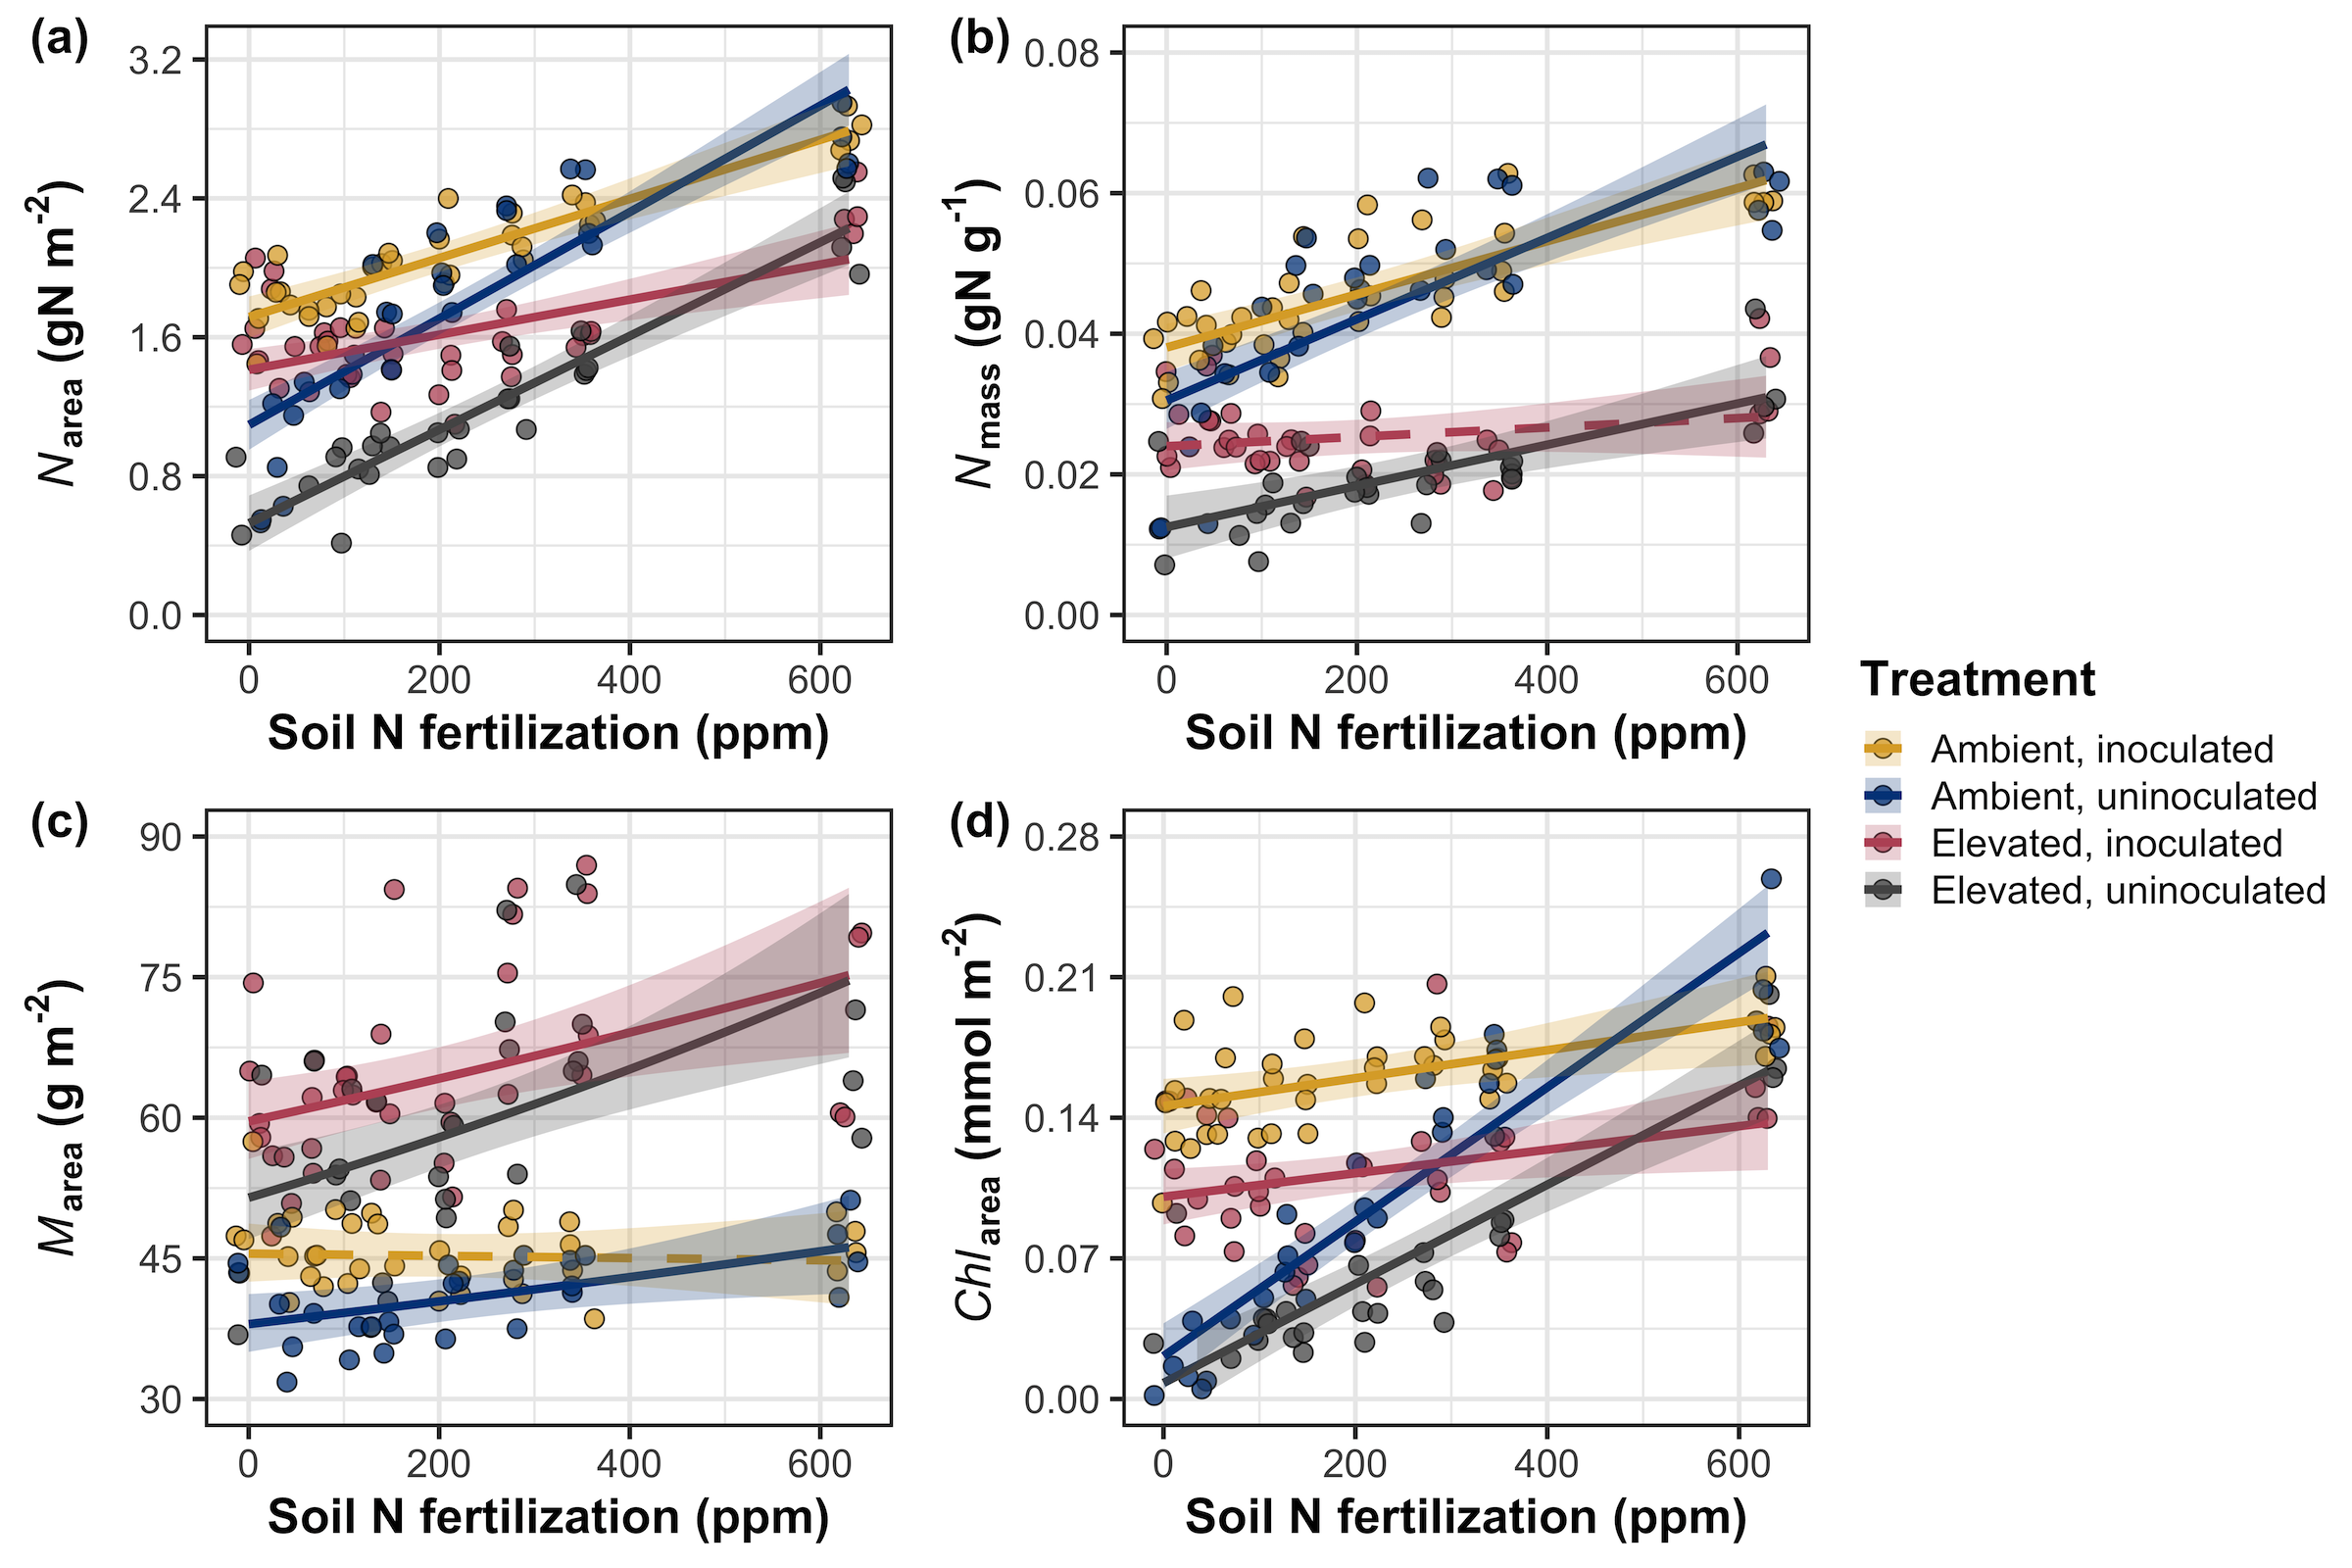
\includegraphics[scale = 0.0625]{ch5_NxCO2xI/figs/NxCO2xI_fig1_leafN.png}
        \caption[Effects of CO$_2$, fertilization, and inoculation on leaf nitrogen per unit leaf area, leaf nitrogen content, leaf mass per unit leaf area, and chlorophyll content per unit leaf area.]{Effects of CO$_2$, fertilization, and inoculation on leaf nitrogen per unit leaf area (a), leaf nitrogen content (b), leaf mass per unit leaf area (c), and chlorophyll content per unit leaf area (d). Soil nitrogen fertilization is represented on the x-axis in all panels. Yellow points and trendlines indicate inoculated individuals grown under ambient CO$_2$, blue points and trendlines indicate uninoculated individuals grown under ambient CO$_2$, red points and trendlines indicate inoculated individuals grown under elevated CO2, and grey points indicate uninoculated individuals grown under elevated CO$_2$. Solid trendlines indicate regression slopes that are different from zero (\textit{p} < 0.05), while dashed trendlines indicate slopes that are not distinguishable from zero (\textit{p} > 0.05).}
        \label{fig:figure5.1}
    \end{figure}
\end{landscape}
\clearpage

\subsection{\textit{Leaf biochemistry and stomatal conductance}}
Elevated CO$_2$ resulted in plants with 16\% lower $V_\mathrm{cmax25}$ (\textit{p} < 0.001; Table 2) and 10\% lower $J_\mathrm{max25}$ (\textit{p} = 0.014; Table 2) as compared to those grown under ambient CO$_2$, but did not influence $R_\mathrm{d25}$ (\textit{p} = 0.613; Table 2). A relatively stronger downregulation in $V_\mathrm{cmax25}$ than $J_\mathrm{max25}$ resulted in an 8\% stimulation in $J_\mathrm{max25}$:$V_\mathrm{cmax25}$ under elevated CO$_2$ (\textit{p} < 0.001; Table 2; Fig. 2E). The downregulatory effect of CO$_2$ on $V_\mathrm{cmax25}$ and $J_\mathrm{max25}$ was not modified across the fertilization gradient (CO$_2$-by-fertilization interaction: \textit{p} = 0.185, \textit{p} = 0.389 for $V_\mathrm{cmax25}$ and $J_\mathrm{max25}$, respectively; Table 2; Fig. 2A, 2C) or between inoculation treatments (CO$_2$-by-inoculation interaction: \textit{p} = 0.799 and \textit{p} = 0.714 for $V_\mathrm{cmax25}$ and $J_\mathrm{max25}$, respectively; Table 2). However, a strong interaction between fertilization and inoculation (fertilization-by-inoculation interaction: p $\le$ 0.001 in all cases; Table 2) indicated that the general positive effect of increasing fertilization on $V_\mathrm{cmax25}$ (\textit{p} < 0.001; Table 2), $J_\mathrm{max25}$ (\textit{p} < 0.001; Table 2), and $R_\mathrm{d25}$ (\textit{p} = 0.015; Table 2) was only observed in uninoculated pots (Tukey: \textit{p} $\le$ 0.001 in all cases), as there was no apparent effect of fertilization on $V_\mathrm{cmax25}$ (Tukey: \textit{p} = 0.456), $J_\mathrm{max25}$ (Tukey: \textit{p} = 0.180), or $R_\mathrm{d25}$ (Tukey: \textit{p} = 0.443) in inoculated pots (Figs. 2B, 2D, 2F, 2H). A relatively stronger positive effect of increasing fertilization on $V_\mathrm{cmax25}$ than $J_\mathrm{max25}$ resulted in a general reduction in $J_\mathrm{max25}$:$V_\mathrm{cmax25}$ with increasing fertilization (\textit{p} < 0.001), though this pattern was only seen in uninoculated pots (Tukey: \textit{p} = 0.003) and not inoculated plants (Tukey: \textit{p} > 0.05).

Elevated CO$_2$ reduced stomatal conductance by 20\% (\textit{p} < 0.001; Table 2) compared to ambient CO$_2$, but this downregulation did not influence stomatal limitation of photosynthesis (\textit{p} = 0.355; Table 2). As with $V_\mathrm{cmax25}$ and $J_\mathrm{max25}$, the downregulation of stomatal conductance due to elevated CO$_2$ was not modified across the fertilization gradient (CO$_2$-by-fertilization interaction: \textit{p} = 0.141; Table 2) or between inoculation treatments (CO$_2$-by-inoculation interaction: \textit{p} = 0.179; Table 2). Fertilization also did not modify the general null effect of CO$_2$ on stomatal limitation (CO$_2$-by-fertilization interaction: \textit{p} = 0.554; Table 2), although an interaction between CO$_2$ and inoculation (CO$_2$-by-inoculation interaction: \textit{p} = 0.043; Table 2) indicated that inoculation increased stomatal limitation under ambient CO$_2$ (Tukey: \textit{p} = 0.021), but not under elevated CO$_2$ (Tukey: \textit{p} > 0.999). An interaction between inoculation and fertilization on stomatal conductance (fertilization-by-inoculation interaction: \textit{p} < 0.001; Table 2) indicated that increasing fertilization increased stomatal conductance in uninoculated pots (Tukey: \textit{p} = 0.003) but decreased stomatal conductance in inoculated pots (Tukey: \textit{p} = 0.021). The similar in magnitude, but opposite direction, trend in the effect of increasing fertilization on stomatal conductance between inoculation treatments likely drove a null general response of stomatal conductance to increasing fertilization (\textit{p} = 0.642; Table 2).

\newpage
\begin{landscape}
    \begin{table}
    \centering
    \caption{Effects of soil nitrogen fertilization, inoculation, and CO$_2$ on leaf biochemistry}
    \resizebox{\columnwidth}{!}{
        \begin{tabular}{p{3cm}p{0.5cm}p{1.75cm}p{1.5cm}p{1.5cm}p{1.75cm}p{1.5cm}p{1.5cm}p{1.75cm}p{1.5cm}p{1.5cm}}
            && 
            \multicolumn{3}{l}{$V_{\mathrm{cmax25}}$} 
            & \multicolumn{3}{l}{$J_{\mathrm{max25}}$} 
            & \multicolumn{3}{l}{$R_{\mathrm{d25}}$} 
            \\
            \hline 
            & 
            \multicolumn{1}{r}{df} 
            & \multicolumn{1}{r}{Coefficient}   & \multicolumn{1}{r}{$\chi^{2}$}    & \multicolumn{1}{r}{\textit{p}} 
            & \multicolumn{1}{r}{Coefficient}   & \multicolumn{1}{r}{$\chi^{2}$}    & \multicolumn{1}{r}{\textit{p}} 
            & \multicolumn{1}{r}{Coefficient}   & \multicolumn{1}{r}{$\chi^{2}$}    & \multicolumn{1}{r}{\textit{p}} 
            \\ 
            \hline

            (Intercept) & \multicolumn{1}{r}{-} 
            &  \multicolumn{1}{r}{4.36E+01}     & \multicolumn{1}{r}{-}             & \multicolumn{1}{r}{-}
            &  \multicolumn{1}{r}{8.30E+01}     & \multicolumn{1}{r}{-}             & \multicolumn{1}{r}{-}
            &  \multicolumn{1}{r}{1.69E+00}     & \multicolumn{1}{r}{-}             & \multicolumn{1}{r}{-} 
            \\

            CO$_2$ & \multicolumn{1}{r}{1}
            & \multicolumn{1}{r}{-7.05E+00}     & \multicolumn{1}{r}{18.039}        & \multicolumn{1}{r}{\textbf{<0.001}}
            & \multicolumn{1}{r}{-9.11E+00}     & \multicolumn{1}{r}{ 6.042}        & \multicolumn{1}{r}{\textbf{0.014}}
            & \multicolumn{1}{r}{ 4.53E-01}     & \multicolumn{1}{r}{ 0.256}        & \multicolumn{1}{r}{0.613} 
            \\


            Inoculation (I) & \multicolumn{1}{r}{1}
            & \multicolumn{1}{r}{5.87E+01}      & \multicolumn{1}{r}{98.579}        & \multicolumn{1}{r}{\textbf{<0.001}}
            & \multicolumn{1}{r}{9.62E+01}      & \multicolumn{1}{r}{85.064}        & \multicolumn{1}{r}{\textbf{<0.001}}
            & \multicolumn{1}{r}{1.04E+00}      & \multicolumn{1}{r}{3.094}         & \multicolumn{1}{r}{\textit{ 0.079}} 
            \\

            Fertilization (N) & \multicolumn{1}{r}{1}
            & \multicolumn{1}{r}{1.32E-01}      & \multicolumn{1}{r}{37.053}        & \multicolumn{1}{r}{\textbf{<0.001}}
            & \multicolumn{1}{r}{2.09E-01}      & \multicolumn{1}{r}{25.356}        & \multicolumn{1}{r}{\textbf{<0.001}}
            & \multicolumn{1}{r}{2.86E-03}      & \multicolumn{1}{r}{5.965}         & \multicolumn{1}{r}{\textbf{ 0.015}} 
            \\

            CO$_2$*I & \multicolumn{1}{r}{1}
            & \multicolumn{1}{r}{-4.65E+00}     & \multicolumn{1}{r}{0.065}         & \multicolumn{1}{r}{0.799}
            & \multicolumn{1}{r}{ 7.84E-01}     & \multicolumn{1}{r}{0.667}         & \multicolumn{1}{r}{0.414}
            & \multicolumn{1}{r}{-5.71E-01}     & \multicolumn{1}{r}{2.563}         & \multicolumn{1}{r}{0.109} 
            \\

            CO$_2$*N & \multicolumn{1}{r}{1}
            & \multicolumn{1}{r}{-3.58E-02}     & \multicolumn{1}{r}{1.758}         & \multicolumn{1}{r}{0.185}
            & \multicolumn{1}{r}{-4.33E-02}     & \multicolumn{1}{r}{0.742}         & \multicolumn{1}{r}{0.389}
            & \multicolumn{1}{r}{-1.55E-03}     & \multicolumn{1}{r}{2.675}         & \multicolumn{1}{r}{0.102} 
            \\

            I*N & \multicolumn{1}{r}{1}
            & \multicolumn{1}{r}{-1.35E-01}     & \multicolumn{1}{r}{60.394}        & \multicolumn{1}{r}{\textbf{<0.001}}
            & \multicolumn{1}{r}{-2.30E-01}     & \multicolumn{1}{r}{57.410}        & \multicolumn{1}{r}{\textbf{<0.001}}
            & \multicolumn{1}{r}{-2.84E-03}     & \multicolumn{1}{r}{12.083}        & \multicolumn{1}{r}{\textbf{0.001}} 
            \\

            CO$_2$*I*N & \multicolumn{1}{r}{1}
            & \multicolumn{1}{r}{2.73E-02}      & \multicolumn{1}{r}{0.748}         & \multicolumn{1}{r}{0.387}
            & \multicolumn{1}{r}{3.46E-02}      & \multicolumn{1}{r}{0.377}         & \multicolumn{1}{r}{0.539}
            & \multicolumn{1}{r}{7.21E-04}      & \multicolumn{1}{r}{0.244}         & \multicolumn{1}{r}{0.622} 
            \\

            \hline

            &&&&&&&&&&
            \\

            && \multicolumn{3}{l}{$J_{\mathrm{max25}}$:$V_\mathrm{cmax25}$} 
            &  \multicolumn{3}{l}{$g_{\mathrm{sw}}$}
            &  \multicolumn{3}{l}{Stomatal limitation}
            \\
            \hline
            & \multicolumn{1}{r}{df}
            & \multicolumn{1}{r}{Coefficient}   & \multicolumn{1}{r}{$\chi^{2}$}    & \multicolumn{1}{r}{\textit{p}}
            & \multicolumn{1}{r}{Coefficient}   & \multicolumn{1}{r}{$\chi^{2}$}    & \multicolumn{1}{r}{\textit{p}} 
            & \multicolumn{1}{r}{Coefficient}   & \multicolumn{1}{r}{$\chi^{2}$}    & \multicolumn{1}{r}{\textit{p}}  
            \\
            \hline

            (Intercept) & \multicolumn{1}{r}{-}
            & \multicolumn{1}{r}{1.92E+00}      & \multicolumn{1}{r}{-}             & \multicolumn{1}{r}{-}
            & \multicolumn{1}{r}{1.95E-01}      & \multicolumn{1}{r}{-}             & \multicolumn{1}{r}{-}
            & \multicolumn{1}{r}{2.12E-01}      & \multicolumn{1}{r}{-}             & \multicolumn{1}{r}{-}
            \\

            CO$_2$ & \multicolumn{1}{r}{1}
            & \multicolumn{1}{r}{ 5.71E-02}     & \multicolumn{1}{r}{92.010}        & \multicolumn{1}{r}{\textbf{<0.001}}
            & \multicolumn{1}{r}{-6.23E-02}     & \multicolumn{1}{r}{9.718}         & \multicolumn{1}{r}{\textbf{ 0.002}}
            & \multicolumn{1}{r}{ 3.91E-02}     & \multicolumn{1}{r}{0.856}         & \multicolumn{1}{r}{0.355} 
            \\

            Inoculation (I) & \multicolumn{1}{r}{1}
            & \multicolumn{1}{r}{-1.79E-01}     & \multicolumn{1}{r}{27.768}        & \multicolumn{1}{r}{\textbf{<0.001}}
            & \multicolumn{1}{r}{ 1.30E-01}     & \multicolumn{1}{r}{22.351}        & \multicolumn{1}{r}{\textbf{<0.001}}
            & \multicolumn{1}{r}{ 7.87E-02}     & \multicolumn{1}{r}{4.582}         & \multicolumn{1}{r}{\textbf{ 0.032}} 
            \\

            Fertilization (N) & \multicolumn{1}{r}{1}
            & \multicolumn{1}{r}{-4.61E-04}     & \multicolumn{1}{r}{28.147}        & \multicolumn{1}{r}{\textbf{<0.001}}
            & \multicolumn{1}{r}{ 2.50E-04}     & \multicolumn{1}{r}{0.066}         & \multicolumn{1}{r}{0.797}
            & \multicolumn{1}{r}{ 2.60E-04}     & \multicolumn{1}{r}{32.218}        & \multicolumn{1}{r}{\textbf{<0.001}} 
            \\

            CO$_2$*I & \multicolumn{1}{r}{1}
            & \multicolumn{1}{r}{ 8.94E-02}     & \multicolumn{1}{r}{2.916}         & \multicolumn{1}{r}{\textit{0.088}}
            & \multicolumn{1}{r}{ 6.69E-02}     & \multicolumn{1}{r}{1.810}         & \multicolumn{1}{r}{0.179}
            & \multicolumn{1}{r}{-7.84E-02}     & \multicolumn{1}{r}{4.093}         & \multicolumn{1}{r}{\textbf{0.043}} 
            \\

            CO$_2$*N & \multicolumn{1}{r}{1}
            & \multicolumn{1}{r}{ 2.35E-04}     & \multicolumn{1}{r}{3.210}         & \multicolumn{1}{r}{\textit{0.073}}
            & \multicolumn{1}{r}{-8.50E-05}     & \multicolumn{1}{r}{2.165}         & \multicolumn{1}{r}{0.141}
            & \multicolumn{1}{r}{-1.24E-04}     & \multicolumn{1}{r}{0.350}         & \multicolumn{1}{r}{0.554} 
            \\

            I*N & \multicolumn{1}{r}{1}
            & \multicolumn{1}{r}{ 3.27E-04}     & \multicolumn{1}{r}{9.607}         & \multicolumn{1}{r}{\textbf{0.002}}
            & \multicolumn{1}{r}{-3.09E-04}     & \multicolumn{1}{r}{14.696}        & \multicolumn{1}{r}{\textbf{<0.001}}
            & \multicolumn{1}{r}{-1.67E-04}     & \multicolumn{1}{r}{2.547}         & \multicolumn{1}{r}{0.110} 
            \\

            CO$_2$*I*N & \multicolumn{1}{r}{1}
            & \multicolumn{1}{r}{-1.66E-04}     & \multicolumn{1}{r}{1.102}         & \multicolumn{1}{r}{0.294}
            & \multicolumn{1}{r}{-8.89E-05}     & \multicolumn{1}{r}{0.234}         & \multicolumn{1}{r}{0.629}
            & \multicolumn{1}{r}{ 1.67E-04}     & \multicolumn{1}{r}{2.231}         & \multicolumn{1}{r}{0.135} 
            \\
            \hline
    \end{tabular}}
    \label{tab:table5.2}
    \end{table}
\begin{singlespace}
\noindent \textsuperscript{$*$}Significance determined using Type II Wald $\chi^{2}$ tests ($\alpha$ = 0.05). \textit{P}-values < 0.05 are in bold, while \textit{p}-values between 0.05 and 0.1 are italicized. Key: $V_\mathrm{cmax25}$ – maximum rate of Rubisco carboxylation at 25\textdegree{}C; $J_\mathrm{max25}$ – maximum rate of electron transport for RuBP regeneration at 25\textdegree{}C, $R_\mathrm{d25}$ - dark respiration at 25\textdegree{}C; $J_{\mathrm{max25}}$:$V_\mathrm{cmax25}$ – the ratio of $J_\mathrm{max25}$ to $V_\mathrm{cmax25}$; $g_{sw}$ - stomatal conductance.
\end{singlespace}
\end{landscape}
\clearpage

\newpage
\begin{figure}
    \centering
    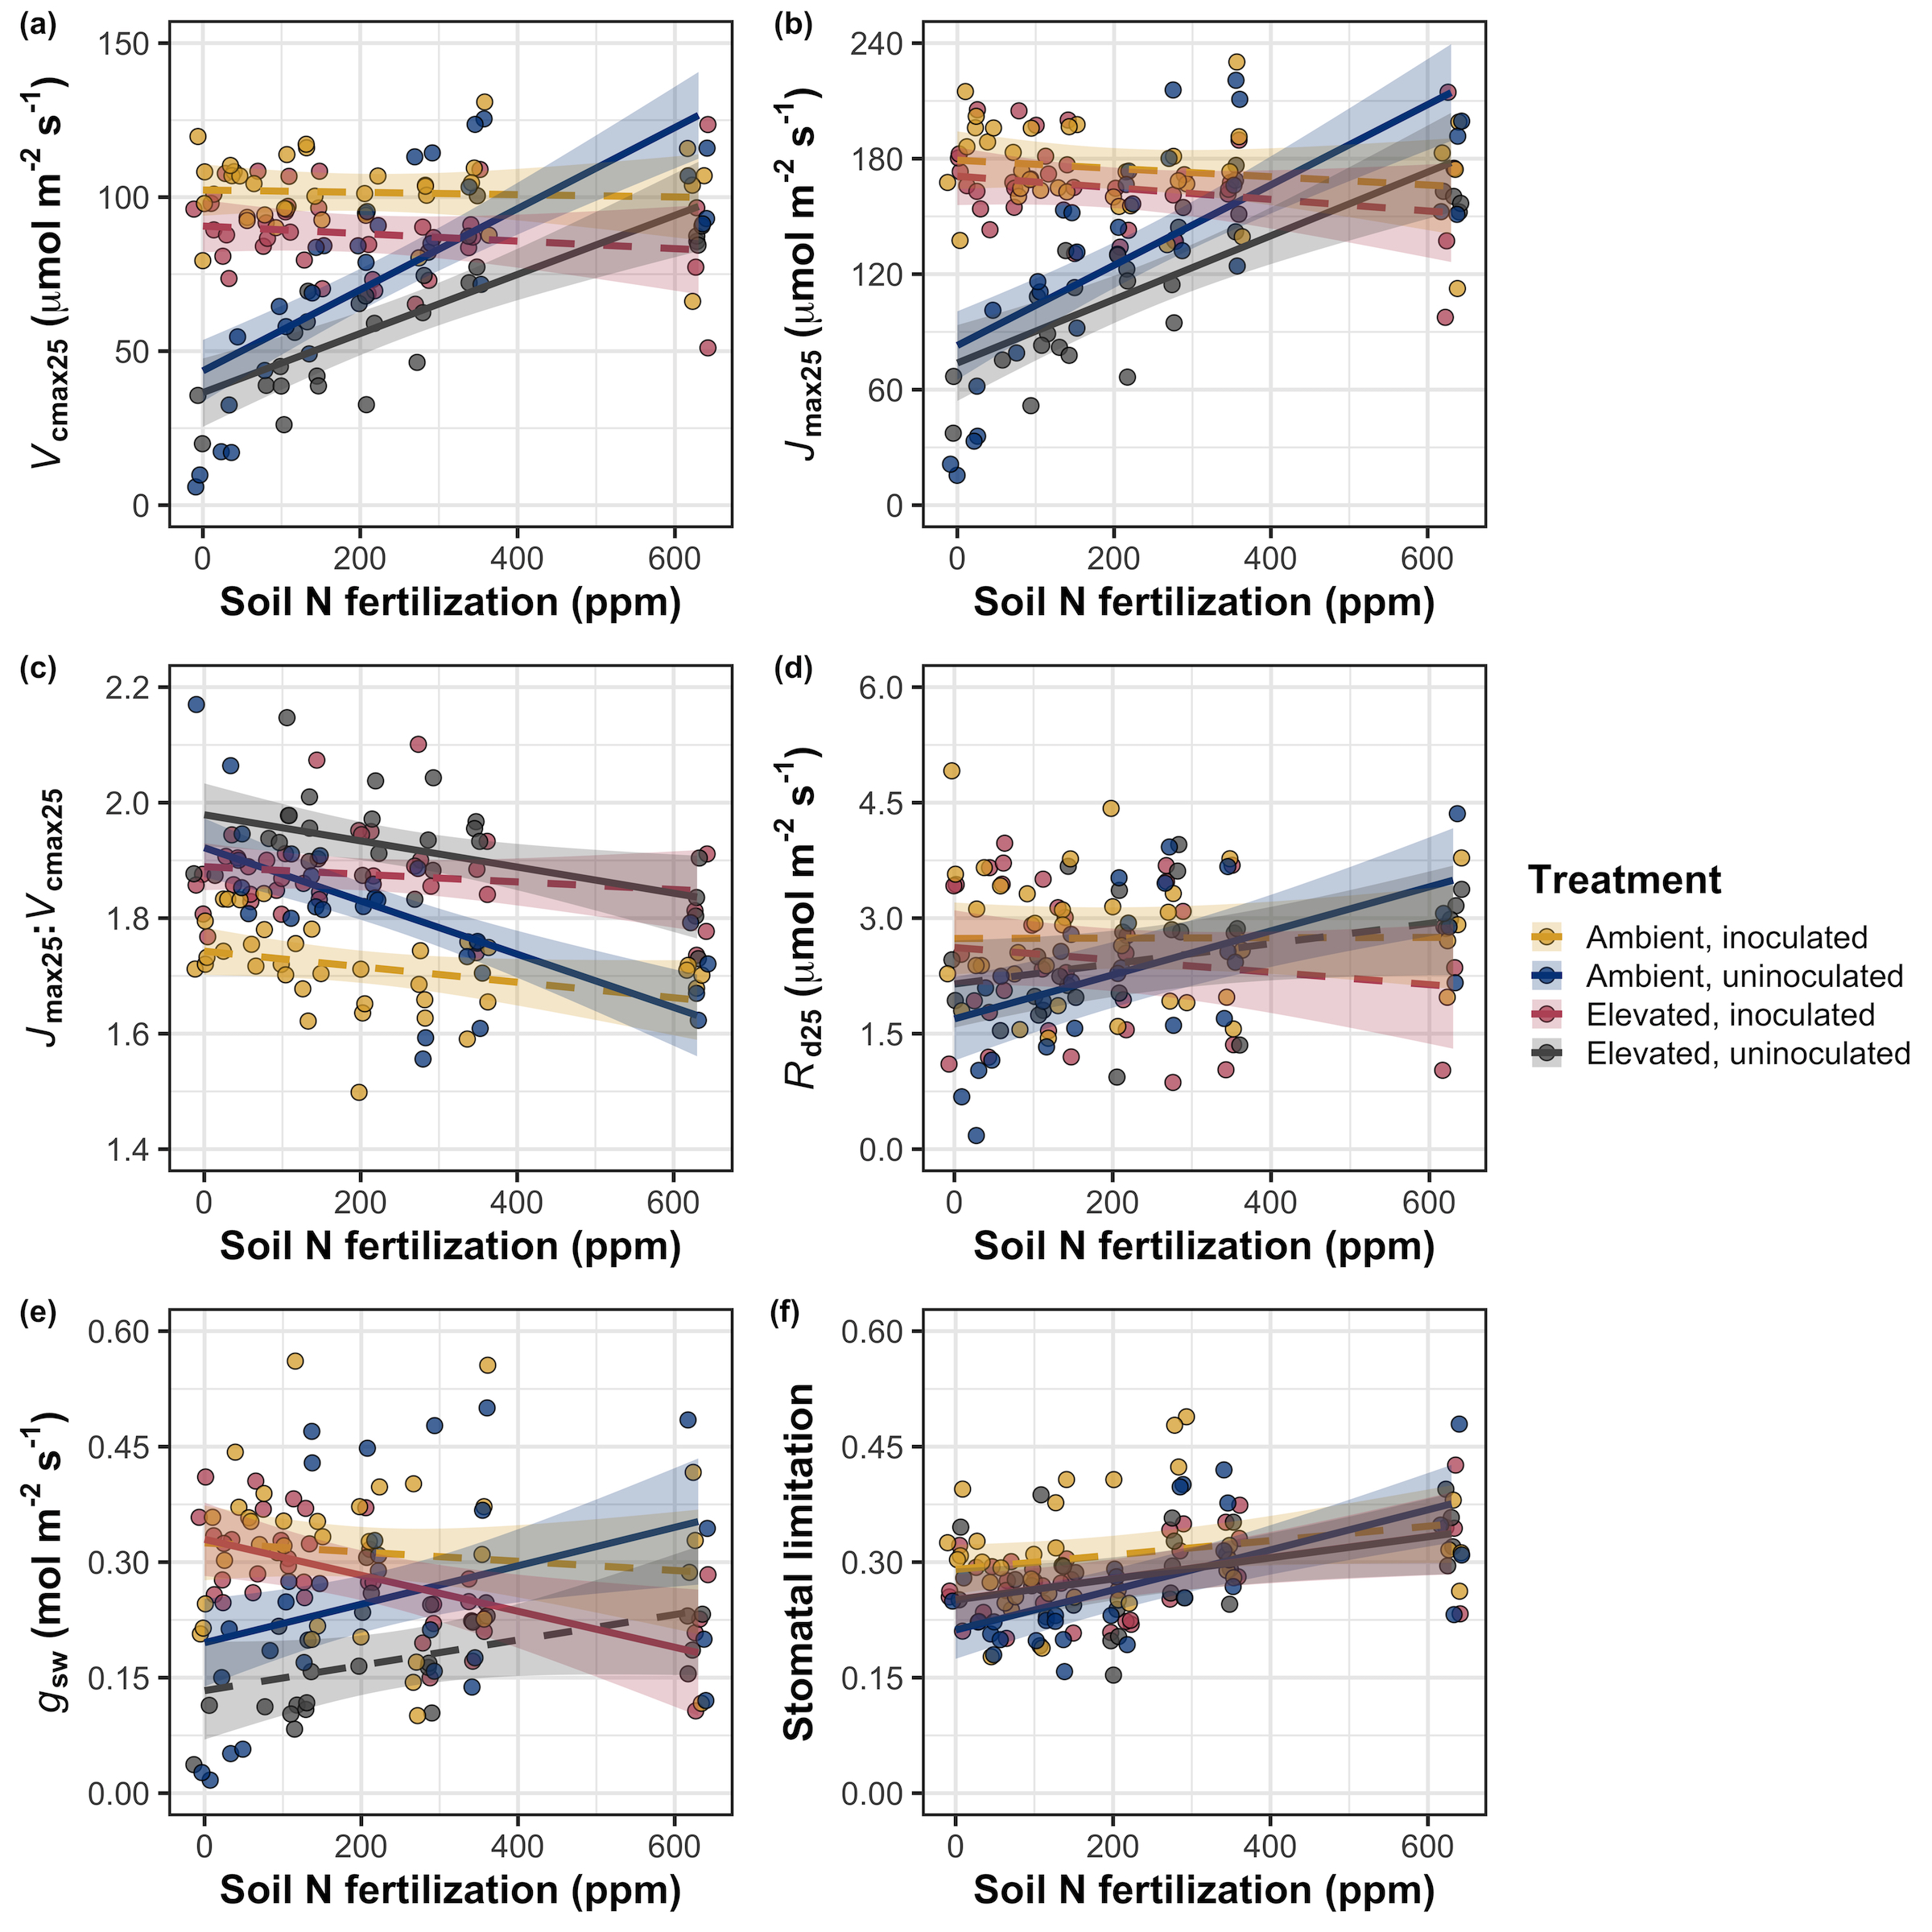
\includegraphics[scale = 0.057]{ch5_NxCO2xI/figs/NxCO2xI_fig2_photo.png}
    \caption[Effects of CO$_2$, fertilization, and inoculation on maximum rate of Rubisco carboxylation, the maximum rate of RuBP regeneration, and the ratio of the maximum rate of RuBP regeneration to the maximum rate of Rubisco carboxylation leaf mass per unit leaf area, dark respiration, stomatal conductance, and stomatal limitation.]{Effects of CO$_2$, fertilization, and inoculation on maximum rate of Rubisco carboxylation (a), the maximum rate of RuBP regeneration (b), and the ratio of the maximum rate of RuBP regeneration to the maximum rate of Rubisco carboxylation leaf mass per unit leaf area (c), dark respiration (d), stomatal conductance (e), and stomatal limitation (f). Soil nitrogen fertilization is represented on the x-axis in all panels. Colored points and trendlines are as explained in Figure 1.}
    \label{fig:figure5.2}
\end{figure}
\clearpage

\subsection{\textit{Leaf nitrogen allocation}}
A relatively stronger downregulation in $N_\mathrm{area}$ than $V_\mathrm{cmax25}$ or $J_\mathrm{max25}$ resulted in an 20\% and 29\% respective stimulation in $\rho_\mathrm{rubisco}$ and $\rho_\mathrm{bioe}$ under elevated CO$_2$ (\textit{p} < 0.001 in both cases; Table 3). There was no apparent CO$_2$ effect on $\rho_\mathrm{light}$ (\textit{p} = 0.700; Table 3), but the strong stimulation in $\rho_\mathrm{rubisco}$ and $\rho_\mathrm{bioe}$ resulted in a 21\% stimulation of $\rho_\mathrm{photo}$ under elevated CO$_2$ (\textit{p} < 0.001; Table 3; Fig. 3A). The stimulation of $\rho_\mathrm{rubisco}$, $\rho_\mathrm{bioe}$, and $\rho_\mathrm{photo}$ due to elevated CO$_2$ was not modified across the fertilization gradient (CO$_2$-by-fertilization interaction: $p_\mathrm{rubisco}$ = 0.269, $p_\mathrm{bioe}$ = 0.298, $p_\mathrm{photo}$ = 0.281; Table 3). A marginal interaction between inoculation and CO2 on $\rho_\mathrm{rubisco}$ and $\rho_\mathrm{photo}$ (CO$_2$-by-inoculation interaction: $p_\mathrm{rubisco}$ = 0.057, $p_\mathrm{photo}$ = 0.057; Table 3) indicated that the general positive effect of inoculation on $\rho_\mathrm{rubisco}$ and $\rho_\mathrm{photo}$ (\textit{p} < 0.001 in both cases; Table 3) was only apparent under ambient CO$_2$ (Tukey: \textit{p} < 0.001 in both cases), with no apparent effect of inoculation under elevated CO$_2$ (Tukey\textsubscript{rubisco}: \textit{p} = 0.200; Tukey\textsubscript{photo}: \textit{p} = 0.147). Inoculation did not modify the stimulation of $\rho_\mathrm{bioe}$ under elevated CO$_2$ (CO$_2$-by-inoculation interaction: \textit{p} = 0.122; Table 3) or the null effect of CO$_2$ on $\rho_\mathrm{bioe}$ (CO$_2$-by-inoculation interaction: \textit{p} = 0.298; Table 3). Strong interactions between fertilization and inoculation on $\rho_\mathrm{rubisco}$, $\rho_\mathrm{bioe}$, and $\rho_\mathrm{photo}$ (fertilization-by-inoculation interaction: \textit{p} < 0.001 in all cases; Table 3) indicated that the general negative effect of increasing fertilization (\textit{p} < 0.001 in all cases; Table 3) was only observed in inoculated pots (Tukey: \textit{p} < 0.001 in all cases), with no apparent effect of fertilization on $\rho_\mathrm{rubisco}$ (Tukey: \textit{p} = 0.612), $\rho_\mathrm{bioe}$ (Tukey: p = 0.544), or $\rho_\mathrm{photo}$ (Tukey: \textit{p} = 0.521; Fig 3B) in uninoculated pots. An additional interaction between fertilization and inoculation on $\rho_\mathrm{light}$ (fertilization-by-inoculation interaction: \textit{p} < 0.001; Table 3) indicated a negative effect of increasing fertilization on $\rho_\mathrm{light}$ in inoculated pots (Tukey: \textit{p} = 0.041), but a positive effect of increasing fertilization in uninoculated pots (Tukey: \textit{p} < 0.001).

The stimulation in $M_\mathrm{area}$ resulted in an 133\% stimulation of $\rho_\mathrm{structure}$ under elevated CO$_2$ (\textit{p} < 0.001; Table 3; Fig 3C). An interaction between fertilization and CO$_2$ (CO$_2$-by-fertilization interaction: \textit{p} = 0.039; Table 3) indicated that the general negative effect of increasing fertilization (p < 0.001; Table 3) on $\rho_\mathrm{structure}$ was marginally stronger under ambient CO$_2$ (Tukey: \textit{p} = 0.055), resulting in a stronger stimulation in $\rho_\mathrm{structure}$ under elevated CO$_2$ with increasing fertilization. A marginal interaction between inoculation and CO$_2$ (CO$_2$-by-inoculation interaction: \textit{p} = 0.057; Table 3) indicated that the general positive effect of inoculation on $\rho_\mathrm{structure}$ (\textit{p} < 0.001; Table 3) was only observed under elevated CO$_2$ (Tukey: \textit{p} < 0.001), with no apparent inoculation effect observed under ambient CO$_2$ (Tukey: \textit{p} = 0.513). Finally, an interaction between fertilization and inoculation (fertilization-by-inoculation interaction: \textit{p} < 0.001; Table 3; Fig. 3D) indicated that, while increasing fertilization generally increased $\rho_\mathrm{structure}$ (\textit{p} < 0.001; Table 3), this response was generally stronger in uninoculated pots (Tukey: \textit{p} = 0.001).

\newpage
\begin{landscape}
    \begin{table}
    \centering
    \caption{Effects of soil N availability, soil pH, species, and $N_\mathrm{area}$ on leaf nitrogen allocation}
    \resizebox{\columnwidth}{!}{
        \begin{tabular}{p{3cm}p{0.5cm}p{1.75cm}p{1.5cm}p{1.5cm}p{1.75cm}p{1.5cm}p{1.5cm}p{1.75cm}p{1.5cm}p{1.5cm}}
            && 
            \multicolumn{3}{l}{$\rho_{\mathrm{rubisco}}$} 
            & \multicolumn{3}{l}{$\rho_{\mathrm{bioe}}$} 
            & \multicolumn{3}{l}{$\rho_{\mathrm{light}}$} 
            \\
            \hline 
            & 
            \multicolumn{1}{r}{df} 
            & \multicolumn{1}{r}{Coefficient}   & \multicolumn{1}{r}{$\chi^{2}$}    & \multicolumn{1}{r}{\textit{p}} 
            & \multicolumn{1}{r}{Coefficient}   & \multicolumn{1}{r}{$\chi^{2}$}    & \multicolumn{1}{r}{\textit{p}} 
            & \multicolumn{1}{r}{Coefficient}   & \multicolumn{1}{r}{$\chi^{2}$}    & \multicolumn{1}{r}{\textit{p}} 
            \\ 
            \hline

            (Intercept) & \multicolumn{1}{r}{-} 
            &  \multicolumn{1}{r}{2.70E-01}     & \multicolumn{1}{r}{-}             & \multicolumn{1}{r}{-}
            &  \multicolumn{1}{r}{5.26E-02}     & \multicolumn{1}{r}{-}             & \multicolumn{1}{r}{-}
            &  \multicolumn{1}{r}{8.48E-03}     & \multicolumn{1}{r}{-}             & \multicolumn{1}{r}{-} 
            \\

            CO$_2$ & \multicolumn{1}{r}{1}
            & \multicolumn{1}{r}{1.42E-01}      & \multicolumn{1}{r}{23.510}        & \multicolumn{1}{r}{\textbf{<0.001}}
            & \multicolumn{1}{r}{3.00E-02}      & \multicolumn{1}{r}{53.899}        & \multicolumn{1}{r}{\textbf{<0.001}}
            & \multicolumn{1}{r}{2.03E-03}      & \multicolumn{1}{r}{0.149}         & \multicolumn{1}{r}{0.700} 
            \\


            Inoculation (I) & \multicolumn{1}{r}{1}
            & \multicolumn{1}{r}{1.83E-01}      & \multicolumn{1}{r}{23.475}        & \multicolumn{1}{r}{\textbf{<0.001}}
            & \multicolumn{1}{r}{2.80E-02}      & \multicolumn{1}{r}{13.860}        & \multicolumn{1}{r}{\textbf{<0.001}}
            & \multicolumn{1}{r}{2.04E-02}      & \multicolumn{1}{r}{147.234}       & \multicolumn{1}{r}{\textbf{<0.001}} 
            \\

            Fertilization (N) & \multicolumn{1}{r}{1}
            & \multicolumn{1}{r}{1.35E-04}      & \multicolumn{1}{r}{16.609}        & \multicolumn{1}{r}{\textbf{<0.001}}
            & \multicolumn{1}{r}{1.22E-05}      & \multicolumn{1}{r}{26.827}        & \multicolumn{1}{r}{\textbf{<0.001}}
            & \multicolumn{1}{r}{3.22E-05}      & \multicolumn{1}{r}{19.378}        & \multicolumn{1}{r}{\textbf{<0.001}} 
            \\

            CO$_2$*I & \multicolumn{1}{r}{1}
            & \multicolumn{1}{r}{-1.07E-01}     & \multicolumn{1}{r}{3.629}         & \multicolumn{1}{r}{\textit{0.057}}
            & \multicolumn{1}{r}{-1.67E-02}     & \multicolumn{1}{r}{2.390}         & \multicolumn{1}{r}{0.122}
            & \multicolumn{1}{r}{-5.33E-03}     & \multicolumn{1}{r}{0.684}         & \multicolumn{1}{r}{0.408} 
            \\

            CO$_2$*N & \multicolumn{1}{r}{1}
            & \multicolumn{1}{r}{-2.16E-04}     & \multicolumn{1}{r}{1.223}         & \multicolumn{1}{r}{0.269}
            & \multicolumn{1}{r}{-3.59E-05}     & \multicolumn{1}{r}{1.085}         & \multicolumn{1}{r}{0.298}
            & \multicolumn{1}{r}{-7.01E-06}     & \multicolumn{1}{r}{0.351}         & \multicolumn{1}{r}{0.553} 
            \\

            I*N & \multicolumn{1}{r}{1}
            & \multicolumn{1}{r}{-4.26E-04}     & \multicolumn{1}{r}{20.045}        & \multicolumn{1}{r}{\textbf{<0.001}}
            & \multicolumn{1}{r}{-6.87E-05}     & \multicolumn{1}{r}{15.458}        & \multicolumn{1}{r}{\textbf{<0.001}}
            & \multicolumn{1}{r}{-4.37E-05}     & \multicolumn{1}{r}{64.042}        & \multicolumn{1}{r}{\textbf{<0.001}} 
            \\

            CO$_2$*I*N & \multicolumn{1}{r}{1}
            & \multicolumn{1}{r}{2.50E-04}      & \multicolumn{1}{r}{3.327}         & \multicolumn{1}{r}{\textit{0.068}}
            & \multicolumn{1}{r}{4.08E-05}      & \multicolumn{1}{r}{2.651}         & \multicolumn{1}{r}{0.103}
            & \multicolumn{1}{r}{1.74E-05}      & \multicolumn{1}{r}{3.735}         & \multicolumn{1}{r}{\textit{0.053}} 
            \\

            \hline

            &&&&&&&&&&
            \\

            &&  \multicolumn{3}{l}{$\rho_\mathrm{photo}$} 
            &   \multicolumn{3}{l}{$\rho_\mathrm{structure}{}^a$} 
            &&& \\
            \hline
            & \multicolumn{1}{r}{df}
            & \multicolumn{1}{r}{Coefficient}   & \multicolumn{1}{r}{$\chi^{2}$}    & \multicolumn{1}{r}{\textit{p}} 
            & \multicolumn{1}{r}{Coefficient}   & \multicolumn{1}{r}{$\chi^{2}$}    & \multicolumn{1}{r}{\textit{p}} 
            \\
            \hline

            (Intercept) & \multicolumn{1}{r}{-}
            & \multicolumn{1}{r}{3.32E-01}      & \multicolumn{1}{r}{-}             & \multicolumn{1}{r}{-}
            & \multicolumn{1}{r}{-2.93E+00}     & \multicolumn{1}{r}{-}             & \multicolumn{1}{r}{-}
            & \multicolumn{1}{r}{}              & \multicolumn{1}{r}{}              & \multicolumn{1}{r}{}
            \\

            CO$_2$ & \multicolumn{1}{r}{1}
            & \multicolumn{1}{r}{1.81E-01}      & \multicolumn{1}{r}{27.651}        & \multicolumn{1}{r}{\textbf{<0.001}}
            & \multicolumn{1}{r}{8.77E-01}      & \multicolumn{1}{r}{229.571}       & \multicolumn{1}{r}{\textbf{<0.001}}
            & \multicolumn{1}{r}{}              & \multicolumn{1}{r}{}              & \multicolumn{1}{r}{} 
            \\

            Inoculation (I) & \multicolumn{1}{r}{1}
            & \multicolumn{1}{r}{2.31E-01}      & \multicolumn{1}{r}{26.238}        & \multicolumn{1}{r}{\textbf{<0.001}}
            & \multicolumn{1}{r}{-2.55E-01}     & \multicolumn{1}{r}{13.872}        & \multicolumn{1}{r}{\textbf{<0.001}}
            & \multicolumn{1}{r}{}              & \multicolumn{1}{r}{}              & \multicolumn{1}{r}{} 
            \\

            Fertilization (N) & \multicolumn{1}{r}{1}
            & \multicolumn{1}{r}{1.76E-04}      & \multicolumn{1}{r}{15.899}        & \multicolumn{1}{r}{\textbf{<0.001}}
            & \multicolumn{1}{r}{-1.51E-03}     & \multicolumn{1}{r}{38.128}        & \multicolumn{1}{r}{\textbf{<0.001}}
            & \multicolumn{1}{r}{}              & \multicolumn{1}{r}{}              & \multicolumn{1}{r}{} 
            \\

            CO$_2$*I & \multicolumn{1}{r}{1}
            & \multicolumn{1}{r}{-1.36E-01}     & \multicolumn{1}{r}{3.671}         & \multicolumn{1}{r}{\textit{0.055}}
            & \multicolumn{1}{r}{-2.99E-01}     & \multicolumn{1}{r}{3.622}         & \multicolumn{1}{r}{\textit{0.057}}
            & \multicolumn{1}{r}{}              & \multicolumn{1}{r}{}              & \multicolumn{1}{r}{} 
            \\

            CO$_2$*N & \multicolumn{1}{r}{1}
            & \multicolumn{1}{r}{-2.72E-04}     & \multicolumn{1}{r}{1.163}         & \multicolumn{1}{r}{0.281}
            & \multicolumn{1}{r}{3.14E-04}      & \multicolumn{1}{r}{4.266}         & \multicolumn{1}{r}{\textbf{0.039}}
            & \multicolumn{1}{r}{}              & \multicolumn{1}{r}{}              & \multicolumn{1}{r}{} 
            \\

            I*N & \multicolumn{1}{r}{1}
            & \multicolumn{1}{r}{-5.37E-04}     & \multicolumn{1}{r}{21.355}        & \multicolumn{1}{r}{\textbf{<0.001}}
            & \multicolumn{1}{r}{7.00E-04}      & \multicolumn{1}{r}{11.025}        & \multicolumn{1}{r}{\textbf{0.001}}
            & \multicolumn{1}{r}{}              & \multicolumn{1}{r}{}              & \multicolumn{1}{r}{} 
            \\

            CO$_2$*I*N & \multicolumn{1}{r}{1}
            & \multicolumn{1}{r}{3.29E-04}      & \multicolumn{1}{r}{4.009}         & \multicolumn{1}{r}{\textbf{0.045}}
            & \multicolumn{1}{r}{4.52E-04}      & \multicolumn{1}{r}{0.669}         & \multicolumn{1}{r}{0.413}
            & \multicolumn{1}{r}{}              & \multicolumn{1}{r}{}              & \multicolumn{1}{r}{} 
            \\
            \hline
    \end{tabular}}
    \label{tab:table5.3}
    \end{table}
\begin{singlespace}
    \noindent \textsuperscript{$*$}Significance determined using Type II Wald $\chi^{2}$ tests ($\alpha$ = 0.05). \textit{P}-values < 0.05 are in bold, while \textit{p}-values between 0.05 and 0.1 are italicized. A superscript “a” is included after trait labels to indicate if models were fit with natural log transformed response variables. Key: df=degrees of freedom, $\rho_\mathrm{rubisco}$ = proportion of leaf N allocated to photosynthesis, $\rho_\mathrm{bioe}$ = proportion of leaf N allocated to bioenergetics, $\rho_\mathrm{light}$=proportion of leaf N allocated to light harvesting proteins, $\rho_\mathrm{photo}$=proportion of leaf N allocated to photosynthesis, $\rho_\mathrm{structure}$=proportion of leaf N allocated to cell wall structural tissue
\end{singlespace}
\end{landscape}
\clearpage

\newpage
\begin{landscape}
    \begin{figure}
        \centering
        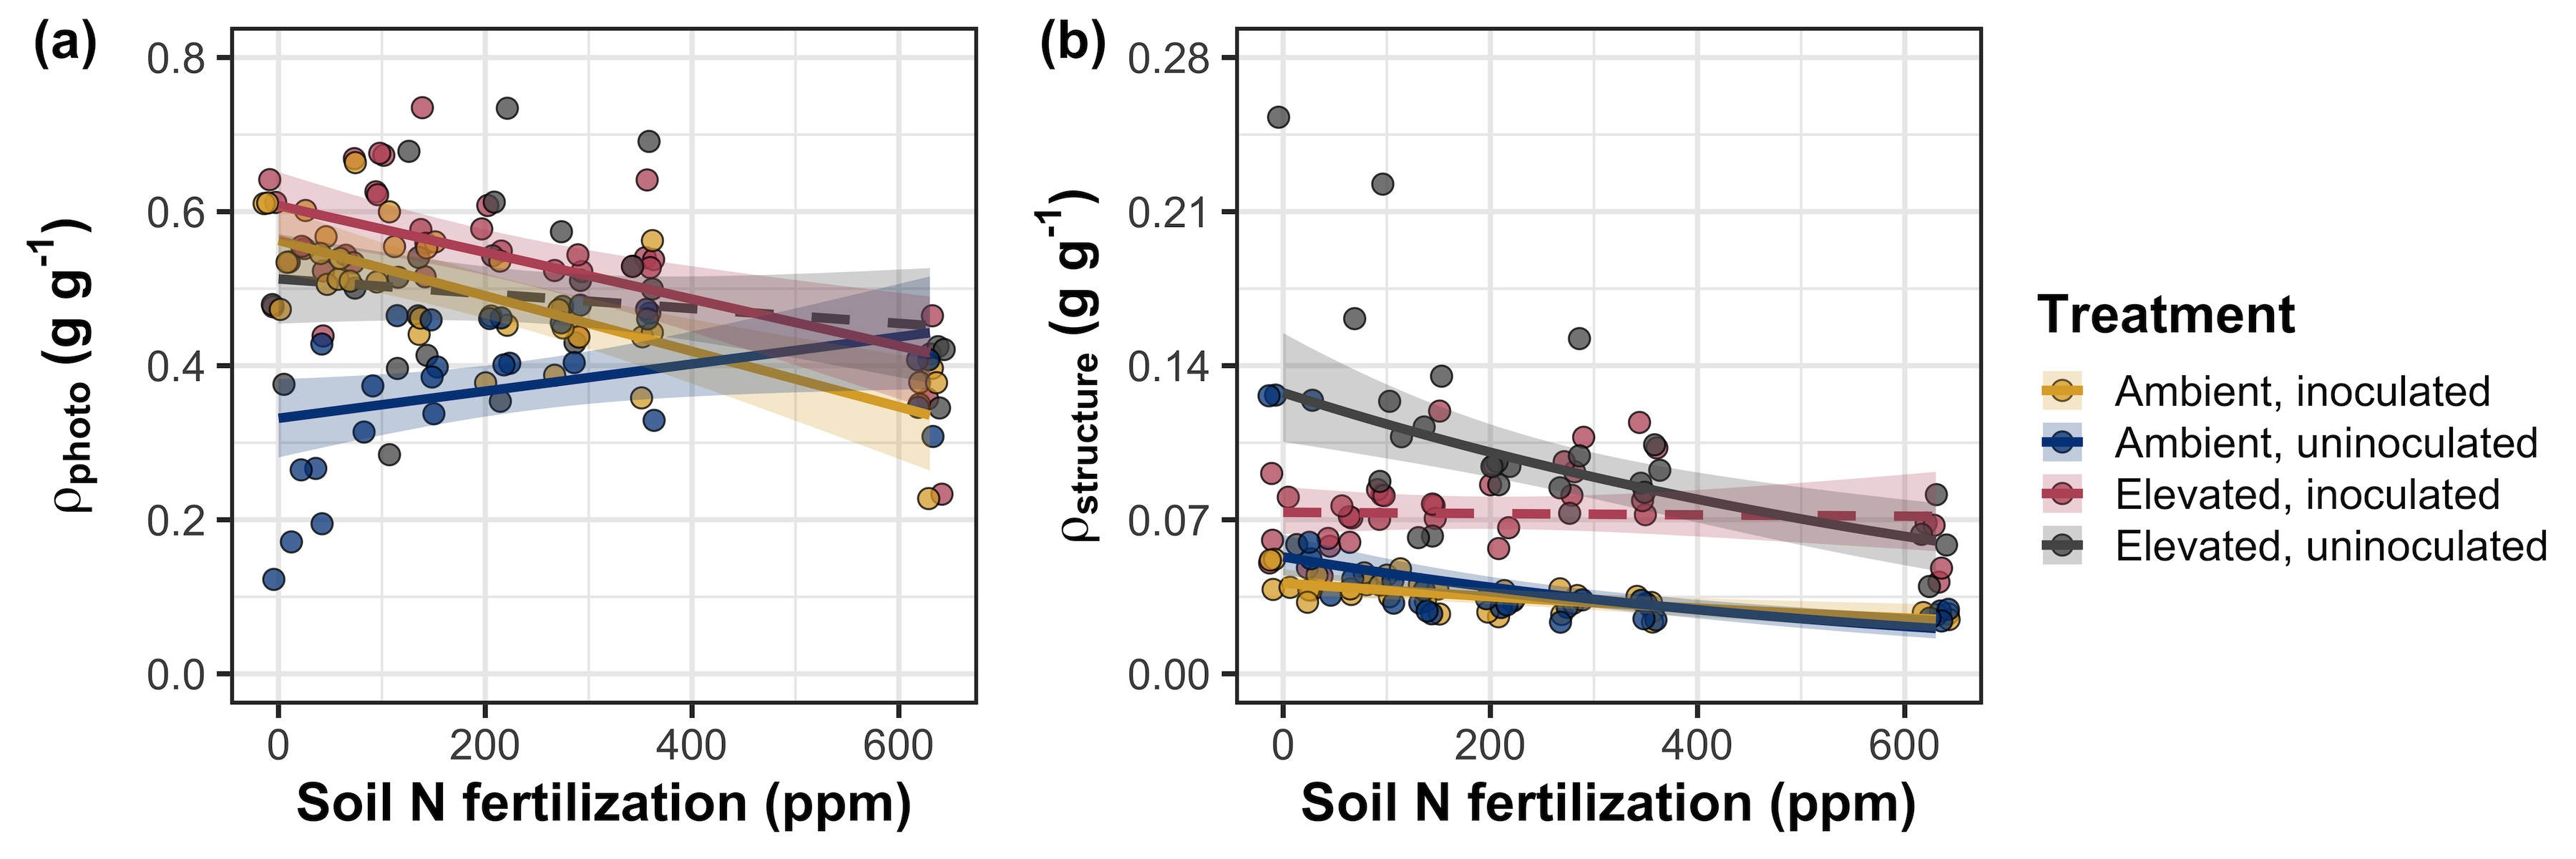
\includegraphics[scale = 0.075]{ch5_NxCO2xI/figs/NxCO2xI_fig3_propN.png}
        \caption[Effects of CO$_2$, fertilization, and inoculation on the relative fraction of leaf nitrogen allocated to photosynthesis and the fraction of leaf nitrogen allocated to structure.]{Effects of CO$_2$, fertilization, and inoculation on the relative fraction of leaf nitrogen allocated to photosynthesis (a) and the fraction of leaf nitrogen allocated to structure (b). Soil nitrogen fertilization is represented on the x-axis in both panels. Colored points and trendlines are as explained in Figure 1.}
        \label{fig:figure5.3}
    \end{figure}
\end{landscape}
\clearpage

\subsection{\textit{Whole plant growth and total leaf area}}
Total leaf area was 51\% greater and total biomass was 102\% greater under elevated CO$_2$ (\textit{p} < 0.001 in both cases; Table 4), a pattern that was enhanced by fertilization (CO$_2$-by-fertilization interaction: \textit{p} < 0.001 in both cases; Table 4; Fig. 4a-b) but was not modified across inoculation treatments (CO$_2$-by-inoculation interaction: $p_{total\_leaf\_area}$ = 0.151, $p_{total\_biomass}$: 0.472; Table 4). Specifically, the general positive effect of increasing fertilization on total leaf area and whole plant biomass (\textit{p} < 0.001 in both cases; Table 4) was stronger under elevated CO$_2$ (Tukey: \textit{p} < 0.001 in both cases). The general positive effect of increasing fertilization on total leaf area was modified by inoculation treatment (fertilization-by-inoculation interaction: \textit{p} < 0.001 in both cases; Table 4), indicating a stronger positive effect of increasing fertilization in uninoculated pots (Tukey: $p_{total\_leaf\_area}$ = 0.002, $p_{total\_biomass}$ = 0.001).

\subsection{\textit{Carbon costs to acquire nitrogen}}
A general 62\% stimulation in $N_\mathrm{cost}$ under elevated CO$_2$ was modified thr-ough a strong three-way interaction between CO$_2$, fertilization, and inoculation (CO$_2$-by-inoculation-by-fertilization interaction: \textit{p} < 0.001; Table 4). This interaction revealed a general negative effect of increasing fertilization on $N_\mathrm{cost}$ (\textit{p} < 0.001; Table 4) that was observed in all treatment combinations (Tukey: \textit{p} < 0.001 in all cases) except for inoculated pots grown under elevated CO$_2$ (Tukey: \textit{p} = 0.779; Fig. 5c). This response also resulted in generally stronger negative effects of increasing fertilization on $N_\mathrm{cost}$ in uninoculated pots grown under elevated CO$_2$ than uninoculated pots grown under ambient CO$_2$ (Tukey: \textit{p} = 0.001) and inoculated pots grown under either ambient CO$_2$ (Tukey: \textit{p} < 0.001) or elevated CO$_2$ (Tukey: \textit{p} < 0.001), while uninoculated pots grown under ambient CO$_2$ had generally stronger negative effects of increasing fertilization on $N_\mathrm{cost}$ than inoculated pots grown under elevated CO$_2$ (Tukey: \textit{p} = 0.002), but not inoculated pots grown under ambient CO$_2$ (Tukey: \textit{p} = 0.216). The general reduction in $N_\mathrm{cost}$ with increasing fertilization and in uninoculated pots were driven by a stronger positive effect of increasing fertilization on $N_\mathrm{wp}$ (denominator of $N_\mathrm{cost}$) than $C_\mathrm{bg}$ (numerator of $N_\mathrm{cost}$), while the general stimulation in $N_\mathrm{cost}$ under elevated CO$_2$ was driven by a stronger positive effect of elevated CO$_2$ on $C_\mathrm{bg}$ than $N_\mathrm{wp}$ (Table 4).

\newpage
\begin{landscape}
    \begin{table}
    \centering
    \caption{Effects of soil N availability, soil pH, species, and $N_\mathrm{area}$ on total leaf area, whole plant biomass, and costs of nitrogen acquisition}
    \resizebox{\columnwidth}{!}{
        \begin{tabular}{p{3cm}p{0.5cm}p{1.75cm}p{1.5cm}p{1.5cm}p{1.75cm}p{1.5cm}p{1.5cm}p{1.75cm}p{1.5cm}p{1.5cm}}
            && 
            \multicolumn{3}{l}{Total leaf area} 
            & \multicolumn{3}{l}{Total biomass} 
            & \multicolumn{3}{l}{$N_\mathrm{cost}$} 
            \\
            \hline 
            & 
            \multicolumn{1}{r}{df} 
            & \multicolumn{1}{r}{Coefficient}   & \multicolumn{1}{r}{$\chi^{2}$}    & \multicolumn{1}{r}{\textit{p}} 
            & \multicolumn{1}{r}{Coefficient}   & \multicolumn{1}{r}{$\chi^{2}$}    & \multicolumn{1}{r}{\textit{p}} 
            & \multicolumn{1}{r}{Coefficient}   & \multicolumn{1}{r}{$\chi^{2}$}    & \multicolumn{1}{r}{\textit{p}} 
            \\ 
            \hline

            (Intercept) & \multicolumn{1}{r}{-} 
            &  \multicolumn{1}{r}{8.78E+01}     & \multicolumn{1}{r}{-}             & \multicolumn{1}{r}{-}
            &  \multicolumn{1}{r}{9.96E-01}     & \multicolumn{1}{r}{-}             & \multicolumn{1}{r}{-}
            &  \multicolumn{1}{r}{8.67E+00}     & \multicolumn{1}{r}{-}             & \multicolumn{1}{r}{-} 
            \\

            CO$_2$ & \multicolumn{1}{r}{1}
            & \multicolumn{1}{r}{3.36E+01}      & \multicolumn{1}{r}{69.291}        & \multicolumn{1}{r}{\textbf{<0.001}}
            & \multicolumn{1}{r}{5.07E-01}      & \multicolumn{1}{r}{131.477}       & \multicolumn{1}{r}{\textbf{<0.001}}
            & \multicolumn{1}{r}{8.75E+00}      & \multicolumn{1}{r}{88.189}        & \multicolumn{1}{r}{\textbf{<0.001}} 
            \\

            Inoculation (I) & \multicolumn{1}{r}{1}
            & \multicolumn{1}{r}{1.88E+02}      & \multicolumn{1}{r}{35.715}        & \multicolumn{1}{r}{\textbf{<0.001}}
            & \multicolumn{1}{r}{7.96E-01}      & \multicolumn{1}{r}{34.264}        & \multicolumn{1}{r}{\textbf{<0.001}}
            & \multicolumn{1}{r}{-1.68E+00}     & \multicolumn{1}{r}{136.343}       & \multicolumn{1}{r}{\textbf{<0.001}} 
            \\

            Fertilization (N) & \multicolumn{1}{r}{1}
            & \multicolumn{1}{r}{9.35E-01}      & \multicolumn{1}{r}{274.199}       & \multicolumn{1}{r}{\textbf{<0.001}}
            & \multicolumn{1}{r}{3.14E-03}      & \multicolumn{1}{r}{269.046}       & \multicolumn{1}{r}{\textbf{<0.001}}
            & \multicolumn{1}{r}{-8.50E-03}     & \multicolumn{1}{r}{80.501}        & \multicolumn{1}{r}{\textbf{<0.001}} 
            \\

            CO$_2$*I & \multicolumn{1}{r}{1}
            & \multicolumn{1}{r}{6.44E+01}      & \multicolumn{1}{r}{2.064}         & \multicolumn{1}{r}{0.151}
            & \multicolumn{1}{r}{-7.69E-02}     & \multicolumn{1}{r}{0.518}         & \multicolumn{1}{r}{0.472}
            & \multicolumn{1}{r}{-8.38E+00}     & \multicolumn{1}{r}{85.237}        & \multicolumn{1}{r}{\textbf{<0.001}} 
            \\

            CO$_2$*N & \multicolumn{1}{r}{1}
            & \multicolumn{1}{r}{5.05E-01}      & \multicolumn{1}{r}{18.655}        & \multicolumn{1}{r}{\textbf{<0.001}}
            & \multicolumn{1}{r}{1.61E-03}      & \multicolumn{1}{r}{16.877}        & \multicolumn{1}{r}{\textbf{<0.001}}
            & \multicolumn{1}{r}{-9.17E-03}     & \multicolumn{1}{r}{1.050}         & \multicolumn{1}{r}{0.306} 
            \\

            I*N & \multicolumn{1}{r}{1}
            & \multicolumn{1}{r}{-3.84E-01}     & \multicolumn{1}{r}{10.804}        & \multicolumn{1}{r}{\textbf{0.001}}
            & \multicolumn{1}{r}{-1.45E-03}     & \multicolumn{1}{r}{15.779}        & \multicolumn{1}{r}{\textbf{<0.001}}
            & \multicolumn{1}{r}{4.20E-03}      & \multicolumn{1}{r}{46.489}        & \multicolumn{1}{r}{\textbf{<0.001}} 
            \\

            CO$_2$*I*N & \multicolumn{1}{r}{1}
            & \multicolumn{1}{r}{-2.97E-03}     & \multicolumn{1}{r}{<0.001}        & \multicolumn{1}{r}{0.990}
            & \multicolumn{1}{r}{-1.14E-04}     & \multicolumn{1}{r}{0.023}         & \multicolumn{1}{r}{0.880}
            & \multicolumn{1}{r}{1.32E-02}      & \multicolumn{1}{r}{18.125}        & \multicolumn{1}{r}{\textbf{<0.001}} 
            \\
            \hline

            &&&&&&&&&&
            \\

            &&  \multicolumn{3}{l}{$C_\mathrm{bg}$} 
            &   \multicolumn{3}{l}{$N_\mathrm{wp}$} 
            &&& \\
            \hline
            & \multicolumn{1}{r}{df}
            & \multicolumn{1}{r}{Coefficient}   & \multicolumn{1}{r}{$\chi^{2}$}    & \multicolumn{1}{r}{\textit{p}} 
            & \multicolumn{1}{r}{Coefficient}   & \multicolumn{1}{r}{$\chi^{2}$}    & \multicolumn{1}{r}{\textit{p}} 
            \\
            \hline

            (Intercept) & \multicolumn{1}{r}{-}
            & \multicolumn{1}{r}{-1.70E+00}     & \multicolumn{1}{r}{-}             & \multicolumn{1}{r}{-}
            & \multicolumn{1}{r}{1.24E-01}      & \multicolumn{1}{r}{-}             & \multicolumn{1}{r}{-}
            & \multicolumn{1}{r}{}              & \multicolumn{1}{r}{}              & \multicolumn{1}{r}{}
            \\

            CO$_2$ & \multicolumn{1}{r}{1}
            & \multicolumn{1}{r}{9.21E-01}      & \multicolumn{1}{r}{84.134}        & \multicolumn{1}{r}{\textbf{<0.001}}
            & \multicolumn{1}{r}{-3.41E-03}     & \multicolumn{1}{r}{23.890}        & \multicolumn{1}{r}{\textbf{<0.001}}
            & \multicolumn{1}{r}{}              & \multicolumn{1}{r}{}              & \multicolumn{1}{r}{} 
            \\


            Inoculation (I) & \multicolumn{1}{r}{1}
            & \multicolumn{1}{r}{1.18E+00}      & \multicolumn{1}{r}{41.030}        & \multicolumn{1}{r}{\textbf{<0.001}}
            & \multicolumn{1}{r}{1.68E-01}      & \multicolumn{1}{r}{134.460}       & \multicolumn{1}{r}{\textbf{<0.001}}
            & \multicolumn{1}{r}{}              & \multicolumn{1}{r}{}              & \multicolumn{1}{r}{} 
            \\

            N fertilization (N) & \multicolumn{1}{r}{1}
            & \multicolumn{1}{r}{3.38E-03}      & \multicolumn{1}{r}{152.248}       & \multicolumn{1}{r}{\textbf{<0.001}}
            & \multicolumn{1}{r}{6.69E-04}      & \multicolumn{1}{r}{529.021}       & \multicolumn{1}{r}{\textbf{<0.001}}
            & \multicolumn{1}{r}{}              & \multicolumn{1}{r}{}              & \multicolumn{1}{r}{} 
            \\

            CO$_2$ * I & \multicolumn{1}{r}{1}
            & \multicolumn{1}{r}{-6.18E-01}     & \multicolumn{1}{r}{8.965}         & \multicolumn{1}{r}{\textbf{0.003}}
            & \multicolumn{1}{r}{3.68E-02}      & \multicolumn{1}{r}{1.190}         & \multicolumn{1}{r}{0.275}
            & \multicolumn{1}{r}{}              & \multicolumn{1}{r}{}              & \multicolumn{1}{r}{} 
            \\

            CO$_2$ * N & \multicolumn{1}{r}{1}
            & \multicolumn{1}{r}{-3.66E-05}     & \multicolumn{1}{r}{1.188}         & \multicolumn{1}{r}{0.276}
            & \multicolumn{1}{r}{1.58E-04}      & \multicolumn{1}{r}{5.915}         & \multicolumn{1}{r}{\textbf{0.015}}
            & \multicolumn{1}{r}{}              & \multicolumn{1}{r}{}              & \multicolumn{1}{r}{} 
            \\

            I * N & \multicolumn{1}{r}{1}
            & \multicolumn{1}{r}{-2.22E-03}     & \multicolumn{1}{r}{22.648}        & \multicolumn{1}{r}{\textbf{<0.001}}
            & \multicolumn{1}{r}{-3.20E-04}     & \multicolumn{1}{r}{55.562}        & \multicolumn{1}{r}{\textbf{<0.001}}
            & \multicolumn{1}{r}{}              & \multicolumn{1}{r}{}              & \multicolumn{1}{r}{} 
            \\

            CO$_2$ * I * N & \multicolumn{1}{r}{1}
            & \multicolumn{1}{r}{8.09E-04}      & \multicolumn{1}{r}{1.109}         & \multicolumn{1}{r}{0.292}
            & \multicolumn{1}{r}{-7.54E-05}     & \multicolumn{1}{r}{0.620}         & \multicolumn{1}{r}{0.431}
            & \multicolumn{1}{r}{}              & \multicolumn{1}{r}{}              & \multicolumn{1}{r}{} 
            \\
            \hline
    \end{tabular}}
    \label{tab:table5.4}
    \end{table}
\begin{singlespace}
    \noindent \textsuperscript{$*$}Significance determined using Type II Wald $\chi^{2}$ tests ($\alpha$ = 0.05). \textit{P}-values < 0.05 are in bold, while \textit{p}-values between 0.05 and 0.1 are italicized. A superscript “a” after trait labels indicates if models were fit using natural log transformed response variables, while a superscript “b” indicates if models were fit using square root transformed variables. Key: df=degrees of freedom
\end{singlespace}
\end{landscape}
\clearpage

\newpage
\begin{figure}
    \centering
    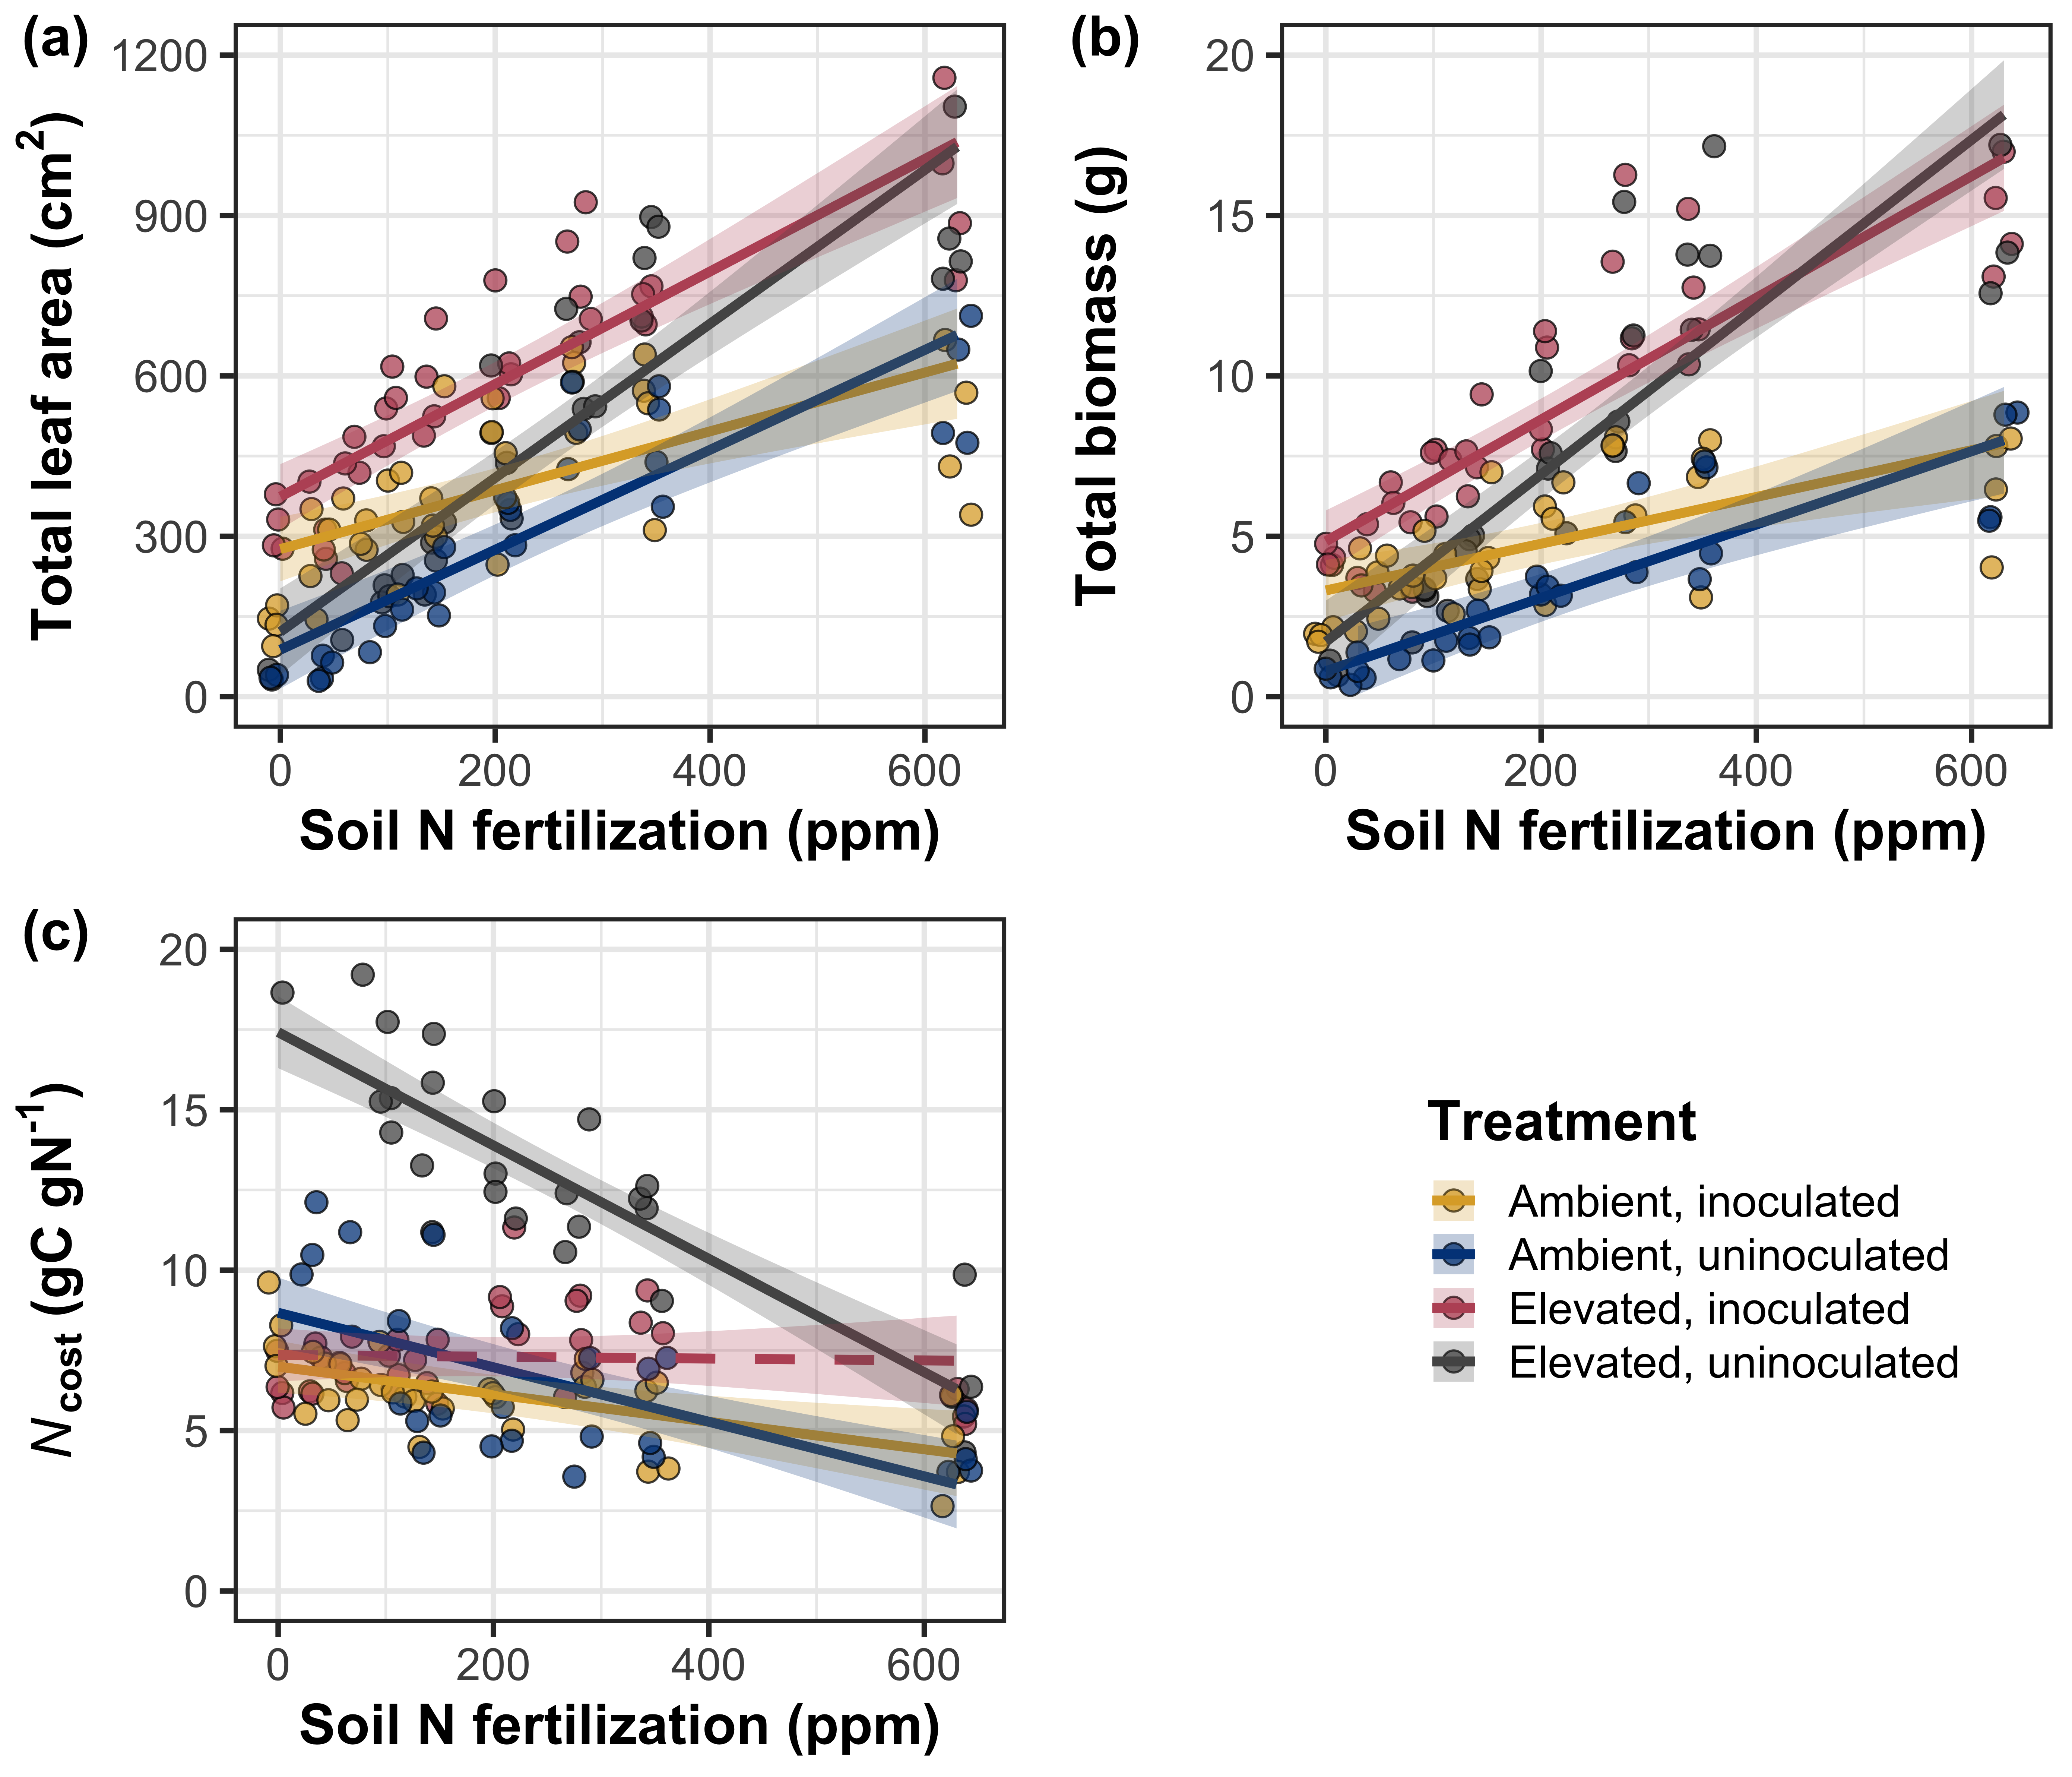
\includegraphics[scale = 0.074]{ch5_NxCO2xI/figs/NxCO2xI_fig4_wholePlant.png}
    \caption[Effects of CO$_2$, fertilization, and inoculation on total leaf area, total biomass, and structural carbon costs to acquire nitrogen.]{Effects of CO$_2$, fertilization, and inoculation on total leaf area (a), total biomass (b), and structural carbon costs to acquire nitrogen (c). Soil nitrogen fertilization is represented continuously on the x-axis in all panels. Colored points and trendlines are as explained in Figure 1.}
    \label{fig:figure5.4}
\end{figure}
\clearpage

\subsection{\textit{Nitrogen fixation}}
Nodule biomass was stimulated by 30\% under elevated CO$_2$ (\textit{p} < 0.001; Table 5), a pattern that was modified across the fertilization gradient (CO$_2$-by-fertilization interaction: \textit{p} = 0.479; Table 5), but not between inoculation treatments (CO$_2$-by-inoculation interaction: p = 0.404; Table 5). Specifically, the general negative effect of increasing fertilization on nodule biomass (\textit{p} < 0.001; Table 5) was stronger under elevated CO$_2$ than ambient CO$_2$ (Tukey: \textit{p} < 0.001; Fig. 5a), which reduced the stimulation in nodule biomass under elevated CO$_2$ with increasing fertilization. A strong interaction between fertilization and inoculation (fertilization-by-inoculation interaction: \textit{p} < 0.001; Table 5) was driven by a stronger negative effect of increasing fertilization in inoculated pots (Tukey: \textit{p} < 0.001; Fig. 5a).

There was no effect of CO$_2$ on nodule: root biomass (\textit{p} = 0.767; Table 5), although an interaction between CO$_2$ and inoculation (CO$_2$-by-inoculation interaction: \textit{p} < 0.001; Table 5) indicated that the general positive effect of inoculation on nodule: root biomass (\textit{p} < 0.001; Table 5) was stronger under ambient CO$_2$ (3129\% increase; Tukey: \textit{p} < 0.001) than elevated CO$_2$ (379\% increase; Tukey: \textit{p} < 0.001; Fig. 5b). The null effect of CO$_2$ on nodule: root biomass was consistently observed across the fertilization gradient (\textit{p} = 0.183; Table 5; Fig. 5b). An interaction between fertilization and inoculation (fertilization-by-inoculation interaction: \textit{p} < 0.001; Table 5) indicated that the general negative effect of increasing fertilization on nodule: root biomass (\textit{p} < 0.001; Table 5) was stronger in inoculated pots (Tukey: \textit{p} < 0.001; Fig. 5b). 

There was no effect of CO$_2$ on \%$N_\mathrm{dfa}$ (\textit{p} = 0.472; Table 5), a pattern that was not modified by inoculation (CO$_2$-by-inoculation interaction: \textit{p} = 0.156; Table 5) or fertilization (CO$_2$-by-fertilization interaction: \textit{p} = 0.099; Table 5). An interaction between fertilization and inoculation (fertilization-by-inoculation interaction: \textit{p} < 0.001; Table 5) indicated that the general negative effect of increasing fertilization on \%$N_\mathrm{dfa}$ (\textit{p} < 0.001; Table 5) was only observed in inoculated pots (Tukey: \textit{p} < 0.001), with no apparent effect of fertilization on \%$N_\mathrm{dfa}$ in uninoculated pots (Tukey: \textit{p} = 0.651; Table 5; Fig. 5c).

\newpage
\begin{landscape}
    \begin{table}
    \centering
    \caption{Effects of soil N availability, soil pH, species, and $N_\mathrm{area}$ on root nodule biomass and plant investments in symbiotic nitrogen fixation}
    \resizebox{\columnwidth}{!}{
        \begin{tabular}{p{3.5cm}p{0.5cm}p{1.75cm}p{1.5cm}p{1.5cm}p{1.75cm}p{1.5cm}p{1.5cm}p{1.75cm}p{1.5cm}p{1.5cm}}
            && 
            \multicolumn{3}{l}{Root nodule biomass\textsuperscript{b}} 
            & \multicolumn{3}{l}{Root nodule: root biomass\textsuperscript{b}} 
            & \multicolumn{3}{l}{$\%N_{\mathrm{dfa}}{}^b$} 
            \\
            \hline 
            &
            \multicolumn{1}{r}{df} 
            & \multicolumn{1}{r}{Coefficient}       & \multicolumn{1}{r}{$\chi^{2}$}    & \multicolumn{1}{r}{\textit{p}} 
            & \multicolumn{1}{r}{Coefficient}       & \multicolumn{1}{r}{$\chi^{2}$}    & \multicolumn{1}{r}{\textit{p}} 
            & \multicolumn{1}{r}{Coefficient}       & \multicolumn{1}{r}{$\chi^{2}$}    & \multicolumn{1}{r}{\textit{p}} 
            \\ 
            \hline

            (Intercept) & \multicolumn{1}{r}{-} 
            &  \multicolumn{1}{r}{9.41E-03}     & \multicolumn{1}{r}{-}             & \multicolumn{1}{r}{-}
            &  \multicolumn{1}{r}{1.33E-02}     & \multicolumn{1}{r}{-}             & \multicolumn{1}{r}{-}
            &  \multicolumn{1}{r}{7.48E-01}     & \multicolumn{1}{r}{-}             & \multicolumn{1}{r}{-} 
            \\

            CO$_2$ & \multicolumn{1}{r}{1}
            & \multicolumn{1}{r}{1.20E-01}      & \multicolumn{1}{r}{19.258}        & \multicolumn{1}{r}{\textbf{<0.001}}
            & \multicolumn{1}{r}{9.94E-02}      & \multicolumn{1}{r}{0.087}         & \multicolumn{1}{r}{0.768}
            & \multicolumn{1}{r}{-1.00E-01}     & \multicolumn{1}{r}{0.518}         & \multicolumn{1}{r}{0.472} 
            \\


            Inoculation (I) & \multicolumn{1}{r}{1}
            & \multicolumn{1}{r}{5.74E-01}      & \multicolumn{1}{r}{755.020}       & \multicolumn{1}{r}{\textbf{<0.001}}
            & \multicolumn{1}{r}{5.40E-01}      & \multicolumn{1}{r}{903.691}       & \multicolumn{1}{r}{\textbf{<0.001}}
            & \multicolumn{1}{r}{9.01E+00}      & \multicolumn{1}{r}{955.570}       & \multicolumn{1}{r}{\textbf{<0.001}} 
            \\

            Fertilization (N) & \multicolumn{1}{r}{1}
            & \multicolumn{1}{r}{7.71E-06}      & \multicolumn{1}{r}{84.376}        & \multicolumn{1}{r}{\textbf{<0.001}}
            & \multicolumn{1}{r}{-5.99E-06}     & \multicolumn{1}{r}{258.099}       & \multicolumn{1}{r}{\textbf{<0.001}}
            & \multicolumn{1}{r}{3.64E-04}      & \multicolumn{1}{r}{292.938}       & \multicolumn{1}{r}{\textbf{<0.001}} 
            \\

            CO$_2$*I & \multicolumn{1}{r}{1}
            & \multicolumn{1}{r}{-4.68E-02}     & \multicolumn{1}{r}{0.950}         & \multicolumn{1}{r}{0.330}
            & \multicolumn{1}{r}{-1.38E-01}     & \multicolumn{1}{r}{20.614}        & \multicolumn{1}{r}{\textbf{<0.001}}
            & \multicolumn{1}{r}{-1.44E-01}     & \multicolumn{1}{r}{2.010}         & \multicolumn{1}{r}{0.156} 
            \\

            CO$_2$*N & \multicolumn{1}{r}{1}
            & \multicolumn{1}{r}{-1.59E-04}     & \multicolumn{1}{r}{2.106}         & \multicolumn{1}{r}{0.147}
            & \multicolumn{1}{r}{-1.73E-04}     & \multicolumn{1}{r}{1.773}         & \multicolumn{1}{r}{0.183}
            & \multicolumn{1}{r}{-6.21E-05}     & \multicolumn{1}{r}{2.716}         & \multicolumn{1}{r}{\textit{0.099}} 
            \\

            I*N & \multicolumn{1}{r}{1}
            & \multicolumn{1}{r}{-5.82E-04}     & \multicolumn{1}{r}{44.622}        & \multicolumn{1}{r}{\textbf{<0.001}}
            & \multicolumn{1}{r}{-7.45E-04}     & \multicolumn{1}{r}{133.918}       & \multicolumn{1}{r}{\textbf{<0.001}}
            & \multicolumn{1}{r}{-1.58E-02}     & \multicolumn{1}{r}{231.290}       & \multicolumn{1}{r}{\textbf{<0.001}} 
            \\

            CO$_2$*I*N & \multicolumn{1}{r}{1}
            & \multicolumn{1}{r}{7.26E-05}      & \multicolumn{1}{r}{0.196}         & \multicolumn{1}{r}{0.658}
            & \multicolumn{1}{r}{1.76E-04}      & \multicolumn{1}{r}{2.359}         & \multicolumn{1}{r}{0.125}
            & \multicolumn{1}{r}{2.77E-03}      & \multicolumn{1}{r}{2.119}         & \multicolumn{1}{r}{0.145} 
            \\
            \hline
    \end{tabular}}
    \label{tab:table5.5}
    \end{table}
\begin{singlespace}
    \noindent \textsuperscript{$*$}Significance determined using Type II Wald $\chi^{2}$ tests ($\alpha$ = 0.05). \textit{P}-values < 0.05 are in bold, while \textit{p}-values between 0.05 and 0.1 are italicized. Superscript letters indicate model coefficients fit to square-root (\textsuperscript{b}) transformed data. Key: \%$N_\mathrm{dfa}$=percent nitrogen fixed from the atmosphere.
\end{singlespace}
\end{landscape}
\clearpage

\newpage
\begin{figure}
    \centering
    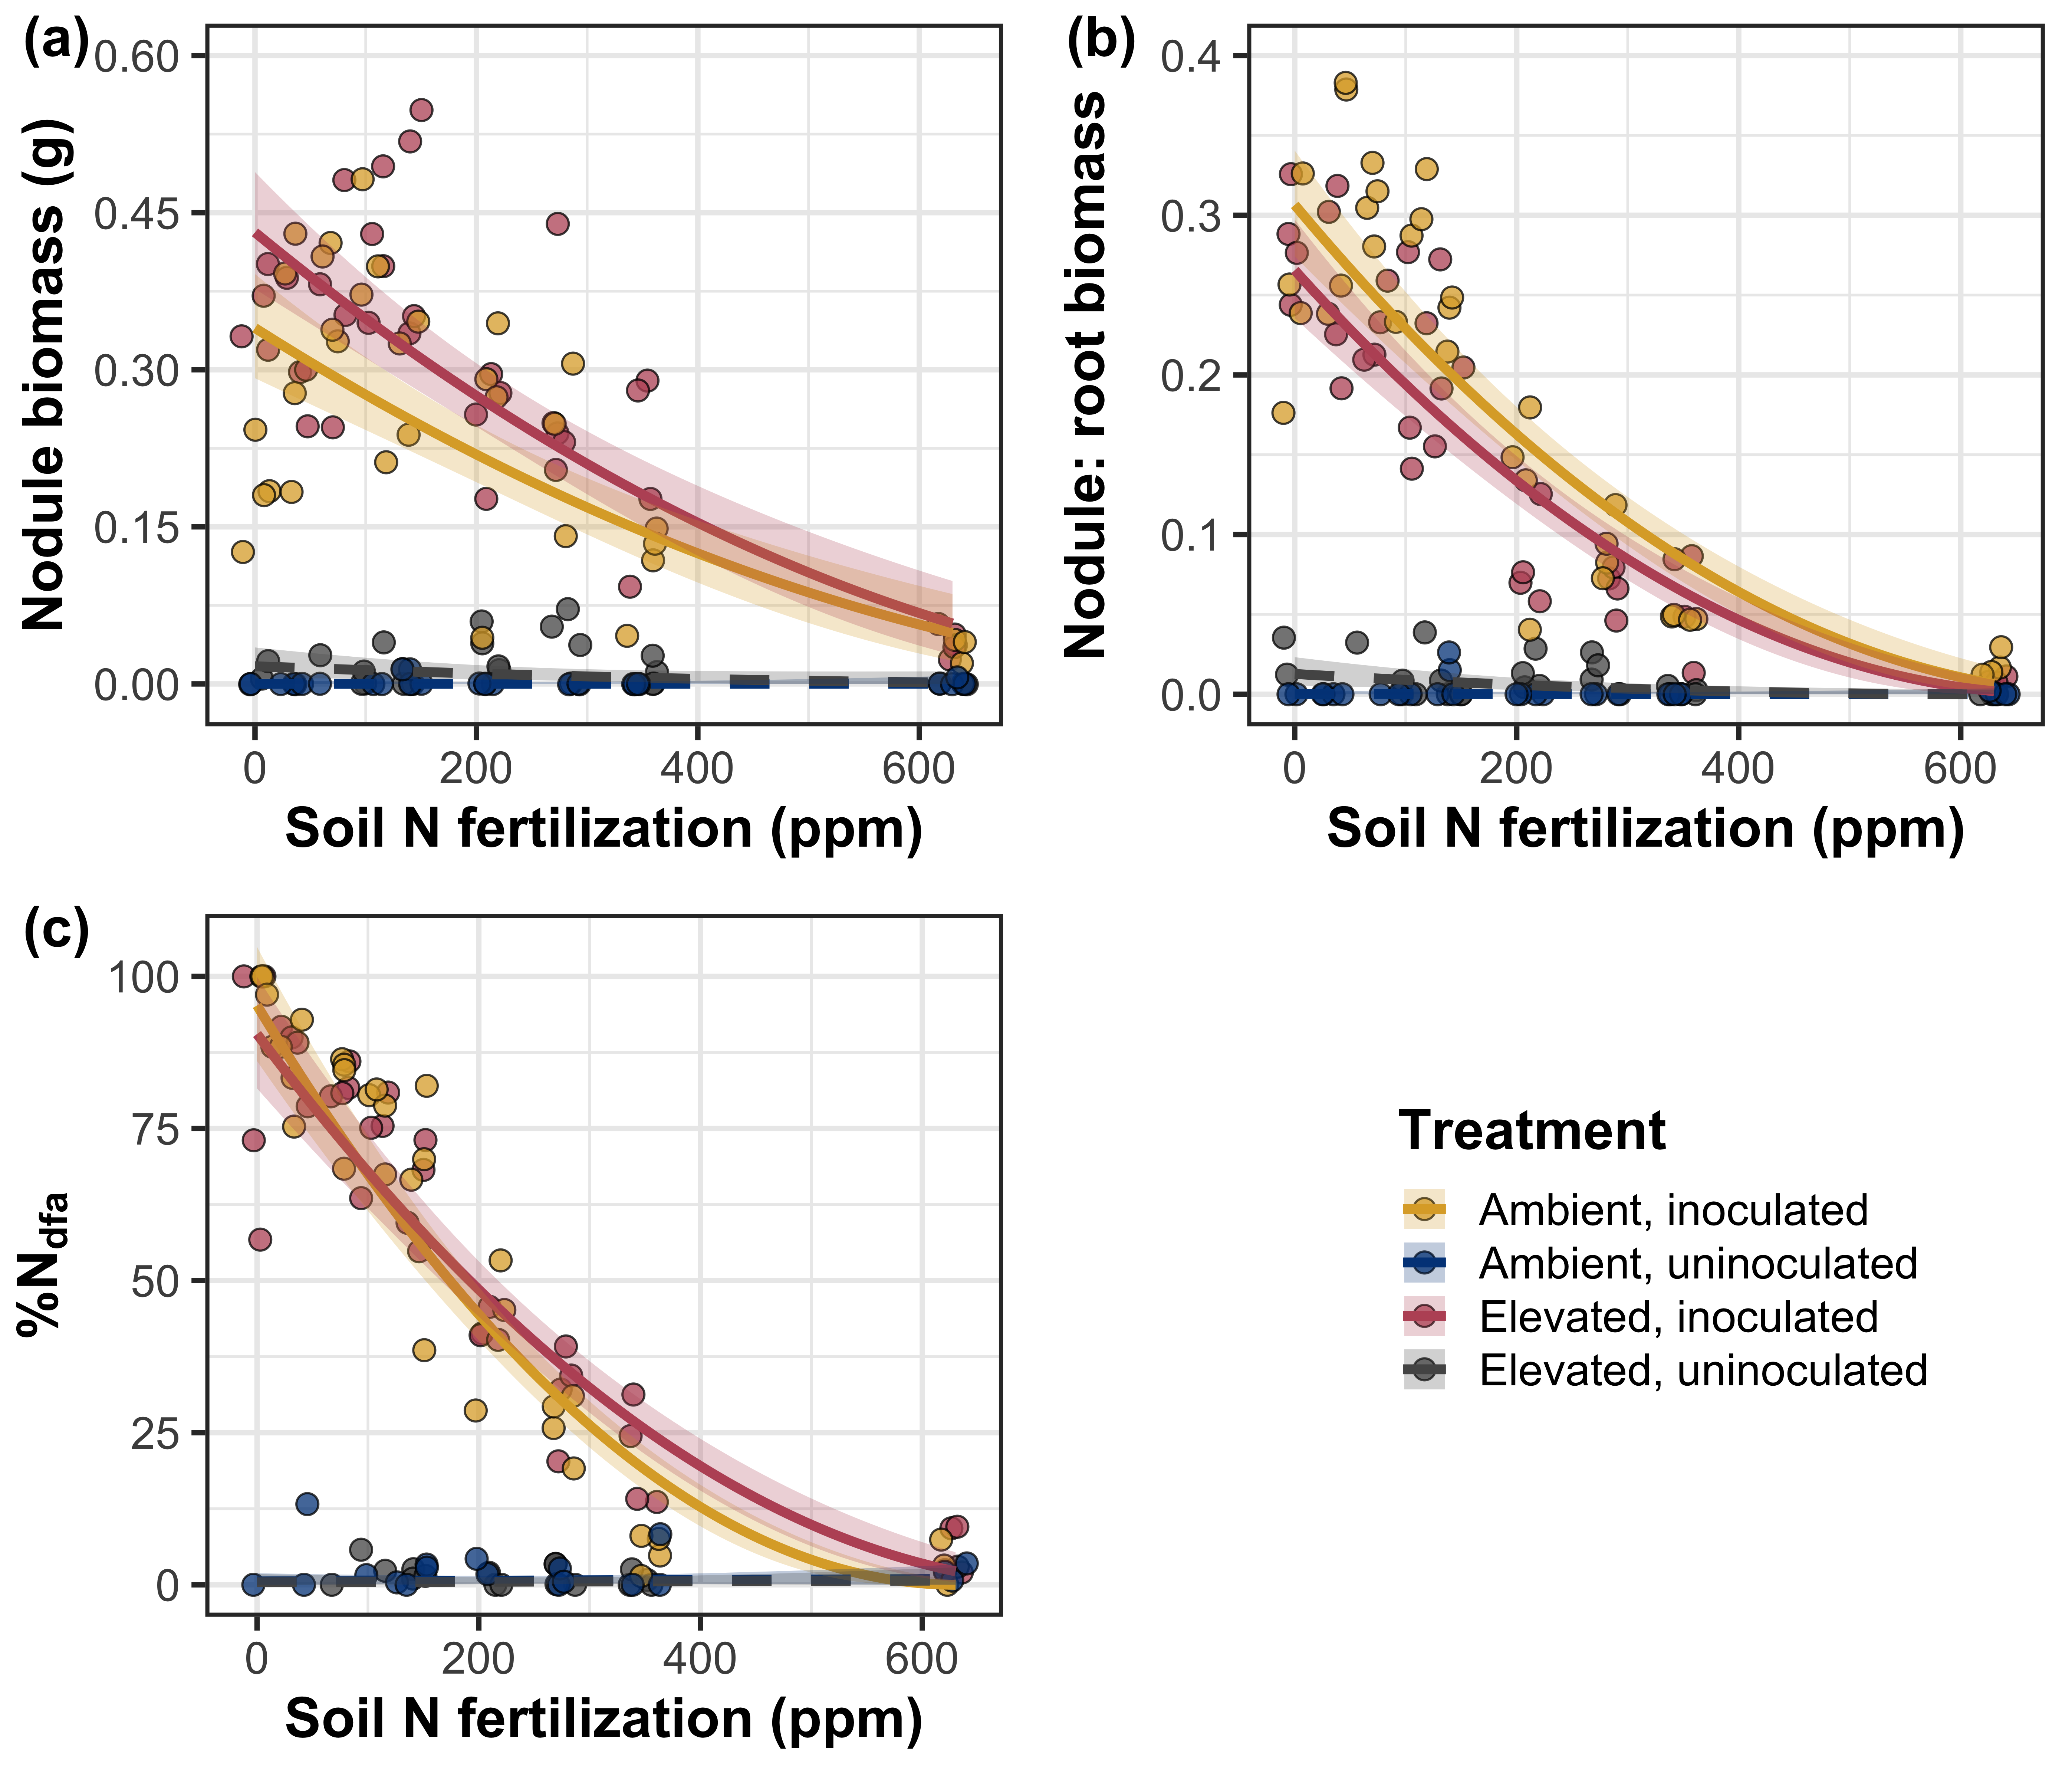
\includegraphics[scale = 0.074]{ch5_NxCO2xI/figs/NxCO2xI_fig5_nFix.png}
    \caption[Effects of CO$_2$, fertilization, and inoculation on nodule biomass, nodule: root biomass, and percent nitrogen fixed from the atmosphere.]{Effects of CO$_2$, fertilization, and inoculation on nodule biomass (a), nodule: root biomass (b), and percent nitrogen fixed from the atmosphere (c). Soil nitrogen fertilization is represented on the x-axis. Yellow points and trendlines indicate inoculated individuals grown under ambient CO$_2$, blue points and trendlines indicate uninoculated individuals grown under ambient CO$_2$, red points and trendlines indicate inoculated individuals grown under elevated CO$_2$, and grey points indicate uninoculated individuals grown under elevated CO$_2$. Solid trendlines indicate slopes that are different from zero (\textit{p} < 0.05), while dashed trendlines indicate slopes that are not different from zero (\textit{p} > 0.05). Curvilinear trendlines occur as a result of back-transforming models where response variables received either a natural log or square root transformation prior to fitting. }
    \label{fig:figure5.5}
\end{figure}
\clearpage

\section{Discussion}
In this study, I determined leaf and whole plant acclimation responses of 7-week \textit{G. max} seedlings grown under two CO$_2$ concentrations, two inoculation treatments, and nine soil nitrogen fertilization treatments in a full-factorial growth chamber experiment. In support of my hypotheses and patterns expected from theory, elevated CO$_2$ reduced $N_\mathrm{area}$, $V_\mathrm{cmax25}$, and $J_\mathrm{max25}$. The relatively stronger downregulation in $V_\mathrm{cmax25}$ than $J_\mathrm{max25}$ under elevated CO$_2$ resulted in a stimulation in $J_\mathrm{max25}$:$V_\mathrm{cmax25}$ under elevated CO$_2$. The downregulation of $V_\mathrm{cmax25}$ and $J_\mathrm{max25}$ under elevated CO$_2$ was similar across fertilization and inoculation treatments, indicating that the CO$_2$ responses were not due to nitrogen limitation. Interestingly, results indicate that elevated CO$_2$ increased the fraction of leaf nitrogen allocated to photosynthesis and structure, leading to a stimulation in nitrogen use efficiency under elevated CO$_2$ despite the apparent downregulation in $N_\mathrm{area}$, $V_\mathrm{cmax25}$, and $J_\mathrm{max25}$. The downregulation in leaf photosynthetic processes under elevated CO$_2$ also corresponded with a strong stimulation in total leaf area and total biomass. Strong stimulations in whole plant growth due to elevated CO$_2$ were generally enhanced with increasing fertilization and were negatively related to structural carbon costs to acquire nitrogen. Inoculation generally did not modify whole plant responses to elevated CO$_2$ across the fertilization gradient, likely due to a strong reduction in root nodulation with increasing fertilization. However, strong positive effects of inoculation on whole plant growth were observed under low fertilization, consistent with our hypothesis. Overall, observed leaf and whole plant acclimation responses to CO$_2$ support hypotheses and patterns expected from photosynthetic least-cost theory, showing that leaf acclimation responses to CO$_2$ were decoupled from soil nitrogen availability and ability to acquire nitrogen via symbiotic nitrogen fixation. Instead, leaf and whole plant acclimation responses to CO$_2$ were driven by optimal resource investment to photosynthetic capacity, where optimal resource investment at the leaf level maximized nitrogen allocation to structures that support whole plant growth.

\subsection{\textit{Soil nitrogen fertilization has divergent effects on leaf and whole plant acclimation responses to CO$_2$}}
Elevated CO$_2$ reduced $N_\mathrm{area}$, $V_\mathrm{cmax25}$, $J_\mathrm{max25}$, and stomatal conductance by 29\%, 16\%, 10\%, and 20\%, respectively (Table \ref{tab:table5.2}). The larger downregulation in $V_\mathrm{cmax25}$ than $J_\mathrm{max25}$ led to an 8\% stimulation in $J_\mathrm{max25}$:$V_\mathrm{cmax25}$ (Table \ref{tab:table5.2}), while the larger downregulation in Narea than $V_\mathrm{cmax25}$ resulted in a 21\% stimulation in the fraction of leaf nitrogen allocated to photosynthesis under elevated CO$_2$. These acclimation responses are directionally consistent with previous studies that have investigated or reviewed leaf acclimation responses to CO$_2$ \shortcite{Drake1997,Makino1997,Ainsworth2002,Ainsworth2005,Ainsworth2007,Smith2013,Smith2020,Poorter2022}, and follow patterns expected from photosynthetic least-cost theory \shortcite{Wright2003,Prentice2014,Smith2019,Smith2020}. Together, the stimulation in $J_\mathrm{max25}$:$V_\mathrm{cmax25}$ and the fraction of leaf nitrogen allocated to photosynthesis, and nitrogen use efficiency under elevated CO$_2$ provide strong support for the idea that leaves were downregulating $V_\mathrm{cmax25}$ in response to elevated CO$_2$ in order to optimally coordinate photosynthesis such that net photosynthesis rates approached becoming equally co-limited by Rubisco carboxylation and RuBP regeneration \shortcite{Chen1993,Maire2012}.

Increasing fertilization and inoculation induced strong positive effects on $N_\mathrm{area}$ (Fig. 1a), $V_\mathrm{cmax25}$ (Fig. \ref{fig:figure5.2}a), $J_\mathrm{max25}$ (Fig. \ref{fig:figure5.2}b). The general positive response of $N_\mathrm{area}$ to increasing fertilization and in inoculated pots was enhanced under ambient CO$_2$, which, paired with the general downregulation in $N_\mathrm{area}$ under elevated CO$_2$, resulted in a stronger downregulation of $N_\mathrm{area}$ under elevated CO$_2$ with increasing fertilization and in inoculated pots (Fig. \ref{fig:figure5.1}a). These patterns suggest that $N_\mathrm{area}$ responses to CO$_2$ were at least partially dependent on soil nitrogen fertilization and nitrogen acquisition strategy. However, the general stimulation in the fraction of leaf nitrogen allocated to Rubisco, bioenergetics, or photosynthesis under elevated CO$_2$ was not modified across the fertilization gradient and was only marginally enhanced in inoculated pots. These patterns suggest that the increased downregulation of $\mathrm{Narea}$ under elevated CO$_2$ with increasing fertilization was not associated with a change in relative investment to photosynthetic tissue. Instead, a stronger downregulation in the fraction of leaf nitrogen allocated to structure under ambient CO$_2$ resulted in a stronger stimulation in $\rho_\mathrm{structure}$ under elevated CO$_2$ with increasing fertilization (Fig. \ref{fig:figure5.3}b), indicating that fertilization shifted relative investment in leaf structural tissue under elevated CO$_2$. These results, combined with a stimulation in PNUE (Fig. SX) and iWUE (Fig. SX) under elevated CO$_2$ that was independent of fertilization or inoculation treatment, provide additional support for the hypothesis that leaf acclimation photosynthetic responses to CO$_2$ were independent of fertilization; though fertilization may contribute to changes in leaf morphology under elevated CO$_2$ through shifts in $M_\mathrm{area}$ \shortcite{Onoda2017,Wang2017,Dong2022a}.

The downregulation in $N_\mathrm{area}$, $V_\mathrm{cmax25}$, and $J_\mathrm{max25}$ under elevated CO$_2$ corresponded with a respective 62\% and 100\% stimulation in total leaf area (Fig. \ref{fig:figure5.4}a) and total biomass (Fig. \ref{fig:figure5.4}b). The stimulation in total leaf area and total biomass under elevated CO$_2$ also corresponded with generally higher structural carbon costs to acquire nitrogen (Fig. \ref{fig:figure5.4}c), a pattern driven by a stimulation in belowground carbon biomass and reduction in whole plant nitrogen biomass. Alone, this result suggests that elevated CO$_2$ reduces plant nitrogen uptake efficiency, which does not explain why plants grown under elevated CO$_2$ generally had higher biomass and total leaf area. However, a strong negative effect of increasing fertilization on structural carbon costs to acquire nitrogen, which were generally similar between CO$_2$ concentrations, was driven by a stronger increase in whole plant nitrogen biomass than belowground carbon biomass. Thus, increases in the positive response of whole plant growth and total leaf area under elevated CO$_2$ with increasing fertilization were likely driven by an increase in nitrogen uptake efficiency, allowing plants to satisfy any increase in whole plant nitrogen demand associated with increased CO$_2$.

Interestingly, these results indicate that the general stimulation in total leaf area and whole plant growth under elevated CO$_2$ was not modified by inoculation despite an apparent general negative effect of inoculation on $N_\mathrm{cost}$. This response could have been due to strong negative effect of increasing fertilization on nodulation (Fig. \ref{fig:figure5.5}), which may have caused the strong increase in the positive effect of elevated CO$_2$ on whole plant growth with increasing fertilization to mask any increase in the positive effect of elevated CO$_2$ on whole plant growth due to inoculation. Reductions in nodulation with increasing fertilization are commonly observed patterns that have been inferred to be a response that allows species optimize nitrogen uptake efficiency as costs to acquire nitrogen via direct uptake become more similar (Fig. \ref{fig:figure5.4}c) \shortcite{Gibson1985,Rastetter2001}. In this study, pairwise comparisons indicated strong positive effects of inoculation on total leaf area and total biomass (158\% increase in total leaf area, 119\% increase in total biomass) under elevated CO$_2$ at 0 ppm N, but no observable inoculation effect on total leaf area or total biomass under elevated CO$_2$ at 350 ppm N or 630 ppm N. While these responses did not generally differ from those observed under ambient CO$_2$, they do confirm the hypothesis that positive effects of inoculation on whole plant growth responses to elevated CO$_2$ would decrease with increasing fertilization.

Combined, results reported here suggest that soil nitrogen availability has a divergent role in modifying leaf and whole plant acclimation responses to CO$_2$. Leaf acclimation responses were generally decoupled from fertilization, while whole plant acclimation responses relied heavily on an increase in nitrogen uptake efficiency and consequent reduction in costs of acquiring nitrogen associated with increasing fertilization. However, whole plant responses to CO$_2$ indicated that fertilization may play a more important role in determining whole plant acclimation responses to CO$_2$ than nitrogen acquisition strategy, although these patterns were likely driven by reductions in nodulation with increasing fertilization. These results suggest that plants acclimate to CO$_2$ in nitrogen-limited systems by minimizing the number of optimally coordinated leaves, and that the downregulation in leaf nitrogen content under elevated CO$_2$ is not a direct response to changes in soil nitrogen availability as previously implied.

\subsection{\textit{Implications for future model development}}
Many terrestrial biosphere models predict photosynthetic capacity through plant functional group-specific linear regressions between $N_\mathrm{area}$ and $V_\mathrm{cmax}$ \shortcite{Rogers2014,Rogers2017a}, which assumes that leaf nitrogen-photosynthesis relationships are constant across growing environments. Our results build on previous work suggesting that leaf nitrogen-photosynthesis relationships dynamically change across growing environments \shortcite{Luo2021,Dong2022a}. Specifically, results from this experiment indicate that CO$_2$ concentration increased the fraction of leaf nitrogen content allocated to photosynthesis, while a general negative effect of increasing fertilization on the fraction of leaf nitrogen content allocated to photosynthesis was dependent on inoculation treatment. Similar increases in $N_\mathrm{area}$, $V_\mathrm{cmax25}$, and $J_\mathrm{max25}$ with increasing fertilization resulted in no change in the fraction of leaf nitrogen allocated to photosynthesis in uninoculated pots, while larger increases in $N_\mathrm{area}$ than $V_\mathrm{cmax25}$ and $J_\mathrm{max25}$ with increasing fertilization decreased the fraction of leaf nitrogen allocated to photosynthesis in inoculated pots (Fig. \ref{fig:figure5.3}a). As inoculated pots were able to access less finite supply of nitrogen across the fertilization gradient, these patterns suggest that constant leaf nitrogen-photosynthesis relationships may only apply in environments where nitrogen is limiting and will likely change with increasing CO$_2$ concentrations. Thus, terrestrial biosphere models that parameterize photosynthetic capacity through linear relationships between $N_\mathrm{area}$ and $V_\mathrm{cmax}$ \shortcite{Rogers2014,Rogers2017a} may be overestimating photosynthetic capacity in systems where nitrogen is not as limiting and may contribute to erroneous model simulations under future CO$_2$ concentrations.

These results also demonstrate that optimal resource investment to photosynthetic capacity defines leaf acclimation responses to elevated CO$_2$, and that these responses were independent of fertilization or inoculation treatment. Current approaches for simulating photosynthetic responses to CO$_2$ generally invoke patterns expected from progressive nitrogen limitation, where the downregulation in $N_\mathrm{area}$, and therefore photosynthetic capacity, due to elevated CO$_2$ are commonly a function of progressive reductions in soil nitrogen availability. Results reported here contradict this formulation, suggesting that the leaf acclimation response is driven by optimal resource investment to photosynthetic capacity and is independent of soil resource supply. Optimality models that leverage principles from optimal coordination and photosynthetic least-cost theories \shortcite{Wang2017,Stocker2020,Scott2022} are capable of capturing such acclimation responses to CO$_2$ \shortcite{Smith2020}, suggesting that the implementation of these models may improve the simulation of photosynthetic processes in terrestrial biosphere models under increasing CO$_2$ concentrations.

\subsection{\textit{Study limitations and future directions}}
There are two study limitations that must be addressed to contextualize patterns observed in this study. First, restricting the volume of belowground substrate via a potted experiment does not adequately replicate belowground environments of natural systems, and therefore may modify effects of soil resource availability and inoculation on plant nitrogen uptake, particularly if pot size limits whole plant growth \shortcite{Poorter2012}. I attempted to minimize the extent of pot size limitation experienced in the first experimental chapters while accounting for the expected stimulation in whole plant growth under elevated CO$_2$ by using 6-liter pots. Despite attempts to minimize growth limitation imposed by pot volume, fertilization and CO$_2$ treatments increased the biomass: pot volume ratio such that all treatment combinations to exceed 1 $\mathrm{g\ L^{-1}}$ biomass: pot volume under high fertilization. The 1 $\mathrm{g\ L^{-1}}$ biomass: pot volume recommendation from \shortciteN{Poorter2012} was designated to avoid growth limitation imposed by pot volume. However, if pot size limitation indeed limited whole plant growth, then structural carbon costs to acquire nitrogen, belowground carbon biomass, whole plant nitrogen biomass, and whole plant biomass should each exhibit strong saturation points with increasing fertilization, which was not observed here. Additionally, a second set of photosynthetic measurements from one week prior to the harvest (6 weeks post-germination) revealed … As pot limitation is expected to decrease net photosynthesis, and focal leaves were of similar ages between the sixth and seventh week, one might expect growth limitation induced by constricted pot volume to result in a dampened effect of inoculation and fertilization on net photosynthesis, $V_\mathrm{cmax}$, and $J_\mathrm{max25}$. Analyses from the sixth week of development revealed … Additionally, analyses revealed a stronger/weaker downregulation in $V_\mathrm{cmax25}$ and $J_\mathrm{max25}$ on week 7, though disentangling the causality of this response (i.e. whether due to pot size limitation or simply a stronger acclimation response) would be difficult.

Second, this study evaluated leaf and whole plant responses to CO$_2$ in 7-week seedlings. Given the long-term scale of the progressive nitrogen limitation hypothesis, patterns observed here should be validated in longer-term nitrogen manipulation experiments. Previous work in free air CO$_2$ enrichment experiments show some support for patterns expected from the progressive nitrogen limitation hypothesis \shortcite{Reich2006,Norby2010}, although results are not consistent across experimental sites \shortcite{Finzi2006,Moore2006,Liang2016}. We found some support for patterns expected by the progressive nitrogen limitation hypothesis, namely an increase in plant nitrogen uptake under elevated CO$_2$ \shortcite{Luo2004}, though leaf acclimation responses to CO$_2$ were strongly indicative of optimal resource investment to photosynthetic capacity as expected from photosynthetic least-cost theory \shortcite{Prentice2014,Smith2019,Smith2020}.

\subsection{\textit{Conclusions}}
This study provides strong evidence suggesting that leaf acclimation responses to elevated CO$_2$ did not vary with soil nitrogen fertilization or ability to acquire nitrogen through symbiotic nitrogen fixation. However, whole plant acclimation responses to CO$_2$ were dependent on fertilization, where increasing fertilization increased the positive effect of whole plant growth under elevated CO$_2$. Results also indicate that fertilization played a relatively more important role in modifying whole plant responses to CO$_2$, perhaps due to a reduction in nodulation across the fertilization gradient. These patterns strongly support the hypothesis that leaf and whole plant acclimation responses are driven by optimal resource investment to photosynthetic capacity, and that leaf acclimation responses to CO$_2$ were not modified by changes in soil nitrogen availability. Additionally, strong interactions between fertilization and inoculation on leaf and whole plant traits indicated positive effects of fertilization on leaf and whole plant traits in uninoculated pots, but null effects of fertilization on leaf and whole plant traits in inoculated pots. These results build on previous work suggesting that constant leaf nitrogen-photosynthesis relationships are dynamic and change across growing environments, calling the use of constant relationships by terrestrial biosphere models into question.


%%%%%%%%%%%%%%%%%%%%%%%%%%%%%%%%%%%%%%%%%%%%%%%%%%
%%%%%%%%%%%%%%%%%%%%%%%%%%%%%%%%%%%%%%%%%%%%%%%%%%
%%%%%%%%%%%%%%%%%%%%%%%%%%%%%%%%%%%%%%%%%%%%%%%%%%
%Conclusion chapter                              %
%%%%%%%%%%%%%%%%%%%%%%%%%%%%%%%%%%%%%%%%%%%%%%%%%%
%%%%%%%%%%%%%%%%%%%%%%%%%%%%%%%%%%%%%%%%%%%%%%%%%%
%%%%%%%%%%%%%%%%%%%%%%%%%%%%%%%%%%%%%%%%%%%%%%%%%%
\chapter{\textbf{Conclusions}}
\noindent The experiments included in this dissertation test mechanisms that drive patterns expected from photosynthetic least-cost theory across various edaphic and climatic gradients. Specifically, I investigate environmental drivers of carbon costs to acquire nitrogen, tradeoffs between nitrogen and water use, and plant acclimation responses to CO$_2$. These experiments provide important empirical data needed to test assumptions made in optimality models that leverage photosynthetic least-cost frameworks, and are among the first manipulative experiments to show support for patterns expected from theory. Below, I summarize main findings of each chapter, synthesize common patterns observed across experiments, and conclude with a few study ideas that I think will help refine our understanding of plant nutrient acquisition and allocation responses to environmental change leveraging patterns predicted by photosynthetic least-cost theory.

In the first experimental chapter, I quantified carbon costs to acquire nitrogen in a species capable of forming associations with symbiotic nitrogen-fixing bacteria (\textit{Glycine max}) and a species not capable of forming such associations (\textit{Gossypium hirsutum}) grown under four soil nitrogen fertilization treatments and four light availability treatments in a full factorial greenhouse experiment. Supporting hypotheses, increasing light availability increased carbon costs to acquire nitrogen in both species due to a larger increase in belowground carbon biomass than whole plant nitrogen biomass. In further support of hypotheses, increasing fertilization decreased carbon costs to acquire nitrogen due to a larger increase in whole plant nitrogen biomass than belowground carbon biomass. Root nodulation data indicated that \textit{G. max} shifted relative carbon allocation from nitrogen fixation to direct uptake with increasing fertilization, which may explain the reduced responsiveness of \textit{G. max} carbon costs to acquire nitrogen across the fertilization gradient. 

Despite evidence that reductions in the response of \textit{G. max} carbon costs to acquire nitrogen to increasing fertilization may have been driven by shifts away from nitrogen fixation with increasing fertilization, I urge caution in assigning causality to the differential response of carbon costs to acquire nitrogen between species. This is because \textit{G. max} and \textit{G. hirsutum} are not phylogenetically related and have different life histories. Differences in life history between the two species limit my ability to assess whether reductions in the negative effect of increasing fertilization on carbon costs to acquire nitrogen in \textit{G. max} were driven by shifts to direct uptake with increasing fertilization. However, these patterns were later confirmed in the fourth experimental chapter, where similar weaker negative effects of increasing fertilization on carbon costs to acquire nitrogen were observed in \textit{G. max} that were inoculated with symbiotic nitrogen-fixing bacteria compared to \textit{G. max} that were left uninoculated across a similar soil nitrogen fertilization gradient.

In the second experimental chapter, I assessed whether changes in soil nitrogen availability or soil pH drove changes in nitrogen-water use tradeoffs predicted by photosynthetic least-cost theory. I measured leaf traits of mature upper canopy deciduous trees growing in a nine-year nitrogen-by-sulfur field manipulation experiment, where experimental sulfur additions were added with intent to acidify plots. Following patterns expected from the theory, increasing soil nitrogen availability was associated with increased leaf nitrogen content, but not net photosynthesis, resulting in an increase in photosynthetic nitrogen use efficiency. In further support of theory, increasing soil nitrogen availability exhibited slight, but nonsignificant, decreases in leaf $C_\mathrm{i}$:$C_\mathrm{a}$ and increases in measures of photosynthetic capacity. Perhaps the strongest evidence for the theory was a strong negative relationship between leaf nitrogen content and leaf $C_\mathrm{i}$:$C_\mathrm{a}$, of which increased with increasing soil nitrogen availability through a stronger increase in leaf nitrogen content than leaf $C_\mathrm{i}$:$C_\mathrm{a}$.

I found no effect of soil pH on nitrogen-water use tradeoffs aside from a marginal reduction in net photosynthesis rates that marginally reduced photosynthetic nitrogen use efficiency with increasing soil pH. Directionally, reductions in photosynthetic nitrogen use efficiency with increasing soil pH were expected per theory; however, this response was driven by no change in leaf nitrogen content and a reduction in net photosynthesis. Theory predicts that these tradeoffs should be driven by no change in net photosynthesis and an increase in leaf nitrogen content. The general null leaf response to changing soil pH may have been due to experimental treatments directly increased soil nitrogen availability and affected soil pH in opposite patterns, suggesting that soil nitrogen availability may be more important in dictating nitrogen-water use tradeoffs than soil pH per se.

In the third experimental chapter, I quantified variance in leaf nitrogen content across a precipitation and soil resource availability gradient in Texan grasslands. Specifically, I measured area-based leaf nitrogen content, components of area-based leaf nitrogen content (leaf mass per unit leaf area, leaf nitrogen per unit dry biomass), leaf $C_\mathrm{i}$:$C_\mathrm{a}$, and the unit cost of acquiring nitrogen relative to water in 520 individuals comprising 57 species. I found that variance in area-based leaf nitrogen content was positively associated with increasing soil nitrogen availability, soil moisture, vapor pressure deficit, and was negatively related to increasing leaf $C_\mathrm{i}$:$C_\mathrm{a}$. Following patterns expected from theory, a path analysis revealed that the positive soil nitrogen-leaf nitrogen relationship was driven by a positive relationship between soil nitrogen availability and the unit cost of acquiring and using nitrogen relative to water, a positive relationship between the unit cost of acquiring and using nitrogen relative to water, and negative relationship between leaf $C_\mathrm{i}$:$C_\mathrm{a}$ and leaf mass per unit leaf area. Interestingly, there was no effect of $C_\mathrm{i}$:$C_\mathrm{a}$ on leaf nitrogen content per unit dry biomass, indicating that variance in area-based leaf nitrogen content across the environmental gradient was driven by a change in leaf morphology and not leaf chemistry.

In the fourth experimental chapter, I quantified leaf and whole plant acclimation responses in \textit{G. max} grown under two atmospheric CO$_2$ levels, with and without inoculation with \textit{Bradyrhizobium japonicum}, and across nine nitrogen fertilization treatments in a full factorial growth chamber experiment. I found strong evidence that leaf nitrogen content, $V_\mathrm{cmax}$, and $J_\mathrm{max}$ were each downregulated under elevated CO$_2$. A stronger downregulation in $V_\mathrm{cmax}$ than $J_\mathrm{max}$ and stronger downregulation in leaf nitrogen content than $V_\mathrm{cmax}$ or $J_\mathrm{max}$ provided strong support suggesting that leaves were acclimating to elevated CO$_2$ by optimizing leaf photosynthetic resource use efficiency to achieve optimal coordination. In striking support of my hypotheses, I find strong evidence suggesting that leaf acclimation responses to elevated CO$_2$ were decoupled from soil nitrogen fertilization and inoculation treatment, despite apparent strong increases in leaf nitrogen content, $V_\mathrm{cmax}$, and $J_\mathrm{max}$ with increasing fertilization and in inoculated pots. These findings contrast the current formulation of photosynthetic processes in terrestrial biosphere models, where many models simulate downregulations in leaf nitrogen content under elevated CO$_2$ as a function of progressive nitrogen limitation.

There are currently two iterations of optimality models that employ the use of patterns expected from photosynthetic least-cost theory, one for C$_3$ species \shortcite{Wang2017,Smith2019,Stocker2020} and one more recently developed for C$_4$ species \shortcite{Scott2022}. In both model variants, costs to acquire and use nitrogen relative to water are held constant using a global dataset of $\delta^{13}$C \shortcite{Cornwell2018}. Throughout experiments, I show strong evidence suggesting that costs to acquire and use nitrogen are dynamic and vary predictably across environmental gradients, and that changes in these costs scale to alter leaf nitrogen-water use tradeoffs and acclimation responses to changing environments in ways predicted through photosynthetic least-cost theory. Thus, while optimality model simulations show good agreement with measured data \shortcite{Smith2019,Stocker2020}, such models may not be capturing an important source of variability in leaf nitrogen-water use tradeoffs by holding costs of resource use constant across environmental gradients.

First principles of photosynthetic least-cost theory suggest that, in a given environment, plants optimize photosynthesis rates by sacrificing inefficient use of a relatively more abundant (and less costly to acquire) resource for more efficient use of a relatively less abundant (and more costly to acquire) resource. Throughout experimental chapters, I show strong support for these patterns across experiments, where increasing soil nitrogen fertilization generally decreased the cost of acquiring nitrogen relative to water, a pattern that scaled to influence leaf nitrogen-water use tradeoffs. I did not find evidence to suggest that soil moisture influenced nitrogen-water use tradeoffs, though this was due to strong covariation between soil moisture and soil nitrogen availability. Overall, findings across experiments provide empirical validation of photosynthetic least-cost theory needed to further develop optimality models and eventually implement such models in terrestrial biosphere model products. Many terrestrial biosphere model products do not include robust frameworks for simulating acclimation responses to changing environmental conditions, and empirical findings shown here provide some support that optimality models that leverage photosynthetic least-cost theory predictions may improve the ability of terrestrial biosphere models to accurately simulate photosynthetic processes.

Many terrestrial biosphere models predict photosynthetic capacity through plant functional group-specific linear regressions between area-based leaf nitrogen content and $V_\mathrm{cmax}$ \shortcite{Rogers2014,Rogers2017a}, which assumes that leaf nitrogen-photosynthesis relationships are constant across growing environments. I found constant leaf nitrogen-photosynthesis relationships with increasing soil nitrogen availability in the nitrogen-by-sulfur field manipulation experiment. However, results from the CO$_2$-by-nitrogen-by-inoculation manipulation experiment indicated that leaf nitrogen-photosynthesis responses to soil nitrogen availability were dependent on whether nitrogen was limiting. Further investigation regarding the effect of soil nitrogen availability in modifying leaf nitrogen-photosynthesis relationships is warranted to better understand the generality of leaf nitrogen photosynthesis relationships across environmental gradients. However, findings from these experiments suggest that representing photosynthetic processes through positive relationships between soil nitrogen availability, leaf nitrogen, and photosynthetic capacity are likely contributing to erroneous errors in model simulations and may explain the high degree of divergence in simulated processes across terrestrial biosphere models \shortcite{Friedlingstein2014,Davies-Barnard2020}.

The experiments included in this dissertation have provided a strong foundation for me to continue growing as a plant physiological ecologist. I envision five primary avenues for future research that build on the work presented here, which are briefly summarized below:

\begin{enumerate}
    \item Manipulative and environmental gradient experiments included here were designed to provide empirical data needed to test photosynthetic least-cost theory assumptions. While these results show promising patterns for patterns expected from photosynthetic least-cost theory, they do not necessarily address whether these patterns follow those simulated by optimality models that leverage photosynthetic least-cost principles. Thus, a clear future direction of these experiments would be to conduct model-data comparisons using data collected here (or similar experiments) to compare against optimality model simulations.
    
    \item Experiments included here explicitly quantify effects of symbiotic nitrogen fixation on carbon costs to acquire nitrogen, nitrogen-water use tradeoffs, and leaf nitrogen-photosynthesis relationships. However, carbon costs to acquire nitrogen also vary in species that associate with different mycorrhizal types \shortcite{Brzostek2014FUN2,Terrer2018}, and dominant mycorrhizal type in an ecosystem has been shown to determine net biogeochemical cycle dynamics in deciduous forests of the northeastern United States \shortcite{Phillips2013}. Thus, future work should consider conducting similar experiments while manipulating mycorrhizal association to better understand how microbial symbioses modify leaf and whole plant acclimation responses to changing environments. 
    
    \item Recent work indicates a high degree of variance in symbiotic nitrogen fixation rates across terrestrial biosphere models \shortcite{Meyerholt2016,Davies-Barnard2020}, perhaps due to nitrogen fixation rates that are implemented across terrestrial biosphere models as a function of temperature \shortcite{Houlton2008}. While energetic costs of nitrogen fixation are dependent on temperature, I show that structural carbon costs to acquire nitrogen via symbiotic nitrogen fixation are driven by factors that influence demand to acquire nitrogen (i.e. CO$_2$, light) and are modified by soil nitrogen supply. The light-by-nitrogen greenhouse experiment was published in \textit{Journal of Experimental Botany}, and a reviewer encouraged future work to include a model-data comparison comparing structural carbon costs to acquire nitrogen measured in the experiment to carbon costs to acquire nitrogen simulated by the FUN biogeochemical model \shortcite{Fisher2010,Brzostek2014FUN2,Allen2020}. Conveniently, FUN calculates carbon costs to acquire nitrogen following the same calculation used in the first and fourth experimental chapter. Conducting such a model-data comparison would be a useful step toward identifying biases in the FUN biogeochemical model, which is currently coupled to several terrestrial biosphere models \shortcite{Clark2011,Shi2016,Lawrence2019,Davies-Barnard2020}.

    \item Carbon costs to acquire nitrogen relative to water were quantified at the leaf level as a function of $\delta^{13}$C and vapor pressure deficit, while structural carbon costs to acquire nitrogen were quantified at the whole plant level as the ratio of belowground carbon allocation per unit whole plant nitrogen biomass. As increasing soil nitrogen availability decreases both leaf and whole plant estimates of costs to acquire and use nitrogen, one might expect leaf and whole plant carbon cost to acquire nitrogen estimates to covary. Future work should consider investigating if leaf and whole plant estimates of carbon costs to acquire nitrogen covary and evaluate whether environmental conditions (or species acquisition strategy) modifies any of this possible covariance. Strong covariance between leaf and whole plant costs of nitrogen acquisition could be a possible avenue to implement frameworks for allowing costs of nitrogen acquisition to vary in optimality models, as the FUN model calculates carbon costs of nitrogen acquisition at the whole plant level.
    
    \item While experiments included here target effects of soil nitrogen availability on carbon costs to acquire nitrogen and associated leaf nitrogen-water use tradeoffs, photosynthetic least-cost theory predicts that plants acclimate their photosynthetic processes by minimizing the summed cost of nutrient (not just nitrogen) and water use. Therefore, the theory would predict similar leaf acclimation responses across soil phosphorus or other nutrient availability gradients. Recent iterations of the FUN biogeochemical cycle includes a framework for determining the carbon and nitrogen cost of acquiring and using phosphorus, which similarly varies in species with different nutrient acquisition strategies \shortcite{Allen2020}. The implementation of this model in a terrestrial biosphere model (E3SM) was also recently shown to improve model performance of ecosystem nutrient limitation \shortcite{Braghiere2022}. As nitrogen and phosphorus commonly co-limit leaf photosynthesis and primary productivity, extending experiments reported here to investigate carbon and nitrogen costs of phosphorus use, and whether these patterns scale to leaf nutrient-water use tradeoffs would be a useful next step in understanding extensions and limitations of photosynthetic least-cost theory.
\end{enumerate}

\noindent The experiments included in this dissertation and the proposed experiments summarized above provide a snapshot view of the things that I have learned throughout my time as a graduate student. I am excited to continue learning and growing as a plant ecophysiologist, ecologist, and scientist, and look forward to continuing along my journey of investigating nutrient acquisition and allocation responses to global change.

%%%%%%%%%%%%%%%%%%%%%%%%%%%%%%%%%%%%%%%%%%%%%%%%%%
%Backmatter -- Bibliography, appendices, etc.%
%%%%%%%%%%%%%%%%%%%%%%%%%%%%%%%%%%%%%%%%%%%%%%%%%%
\backmatter

%%%%%%%%%%%%%%%%%%%%%%%%%%%%%%%%%%%%%%%%%%%%%%%%%%
%Bibliography
%%%%%%%%%%%%%%%%%%%%%%%%%%%%%%%%%%%%%%%%%%%%%%%%%%
\bibliographystyle{chicago}
\addcontentsline{toc}{chapter}{\textbf{References}}
\bibliography{reference_list}

%%%%%%%%%%%%%%%%%%%%%%%%%%%%%%%%%%%%%%%%%%%%%%%%%%
%Appendices
%%%%%%%%%%%%%%%%%%%%%%%%%%%%%%%%%%%%%%%%%%%%%%%%%%
\begin{singlespace}
    \chapter{\textbf{Appendix A: Supplemental material for "Structural carbon costs to acquire nitrogen are determined by nitrogen and light availability in two species with different nitrogen acquisition strategies"}}
\end{singlespace}

\setcounter{table}{0}
\renewcommand{\thetable}{A\arabic{table}}

\setcounter{figure}{0}
\renewcommand{\thefigure}{A\arabic{figure}}

\begin{table}[h!]
    \caption[Summary table containing volumes of compounds used to create modified Hoagland's solutions for each soil nitrogen fertilization treatment]{Summary table containing volumes of compounds used to create modified Hoagland's solutions for each soil nitrogen fertilization treatment. All volumes are expressed as milliliters per liter (mL L$^{-1}$)}
    \label{table:tab.a1}
    \resizebox{\columnwidth}{!}{%
    \begin{tabular}{p{4cm}p{2cm}p{2cm}p{2cm}p{2cm}}
    \hline
    \textbf{Compound}       & \multicolumn{1}{r}{\textbf{0 ppm N}}  & \multicolumn{1}{r}{\textbf{70 ppm N}} & \multicolumn{1}{r}{\textbf{210 ppm N}} & \multicolumn{1}{r}{\textbf{630 ppm N}} \\
    \hline
    1 M NH$_4$H$_2$PO$_4$   & \multicolumn{1}{r}{0}                 & \multicolumn{1}{r}{0.33}              & \multicolumn{1}{r}{1}         & \multicolumn{1}{r}{1}  \\
    2 M KNO$_3$             & \multicolumn{1}{r}{0}                 & \multicolumn{1}{r}{0.67}              & \multicolumn{1}{r}{2}         & \multicolumn{1}{r}{2}  \\
    2 M Ca(NO$_3$)$_2$      & \multicolumn{1}{r}{0}                 & \multicolumn{1}{r}{0.67}              & \multicolumn{1}{r}{2}         & \multicolumn{1}{r}{2}  \\
    1 M NH$_4$NO$_3$        & \multicolumn{1}{r}{0}                 & \multicolumn{1}{r}{0.33}              & \multicolumn{1}{r}{1}         & \multicolumn{1}{r}{0}  \\
    8 M NH$_4$NO$_3$        & \multicolumn{1}{r}{0}                 & \multicolumn{1}{r}{0}                 & \multicolumn{1}{r}{0}         & \multicolumn{1}{r}{2}  \\
    1 M KH$_2$PO$_4$        & \multicolumn{1}{r}{1}                 & \multicolumn{1}{r}{0.67}              & \multicolumn{1}{r}{0}         & \multicolumn{1}{r}{0}  \\
    1 M KCl                 & \multicolumn{1}{r}{4}                 & \multicolumn{1}{r}{1.33}              & \multicolumn{1}{r}{0}         & \multicolumn{1}{r}{0}  \\
    1 M CaCO$_3$            & \multicolumn{1}{r}{4}                 & \multicolumn{1}{r}{3}                 & \multicolumn{1}{r}{0}         & \multicolumn{1}{r}{0} \\
    2 M MgSO$_4$            & \multicolumn{1}{r}{1}                 & \multicolumn{1}{r}{1}                 & \multicolumn{1}{r}{1}         & \multicolumn{1}{r}{1} \\
    10\% Fe-EDTA            & \multicolumn{1}{r}{1}                 & \multicolumn{1}{r}{1}                 & \multicolumn{1}{r}{1}         & \multicolumn{1}{r}{1} \\
    Trace Elements          & \multicolumn{1}{r}{1}                 & \multicolumn{1}{r}{1}                 & \multicolumn{1}{r}{1}         & \multicolumn{1}{r}{1} \\
    \hline
    \end{tabular}%
    }
    \end{table}
\clearpage

\newpage
\begin{table}[]
    \caption[Analysis of variance results exploring species-specific effects of light availability, nitrogen fertilization, and their interactions on the ratio of whole plant biomass to pot volume]{Analysis of variance results exploring species-specific effects of light availability, nitrogen fertilization, and their interactions on the ratio of whole plant biomass to pot volume (g L$^{-1}$)$^*$}
    \label{table:tab.a2}
    \centering
    %\resizebox{\columnwidth}{!}{
        \begin{tabular}{p{0.1cm}p{2.5cm}p{0.5cm}p{1.75cm}p{1.5cm}p{1.5cm}}
         &&&&& 
         \\
         \hline 
         && 
         \multicolumn{1}{r}{df}
         & \multicolumn{1}{r}{Coefficient} & \multicolumn{1}{r}{$\chi^2$} & \multicolumn{1}{r}{\textit{p}}
         \\ 
         \hline
         
         \multicolumn{2}{l}{\textit{G. hirsutum}} &&&&  \\
         & Intercept 
         && \multicolumn{1}{r}{0.740} & \multicolumn{1}{r}{-} & \multicolumn{1}{r}{-} 
         \\
         
         & Light (L)            
         & \multicolumn{1}{r}{1}
         & \multicolumn{1}{r}{-4.23E$-$03}    & \multicolumn{1}{r}{189.581}    & \multicolumn{1}{r}{\textbf{<0.001}}
         \\
         
         & Nitrogen (N)
         & \multicolumn{1}{r}{1} 
         & \multicolumn{1}{r}{7.86E$-$04}    & \multicolumn{1}{r}{17.927}    & \multicolumn{1}{r}{\textbf{<0.001}}
         \\
         
         & L*N
         & \multicolumn{1}{r}{1}            
         & \multicolumn{1}{r}{-6.61E$-$06}     & \multicolumn{1}{r}{4.709}     & \multicolumn{1}{r}{\textbf{0.030}}              
         \\
         &&&&& \\

         \multicolumn{2}{l}{\textit{G. max}} &&&&  \\
         & Intercept 
         && \multicolumn{1}{r}{-0.233} & \multicolumn{1}{r}{-} & \multicolumn{1}{r}{-} 
         \\
         
         & Light (L)            
         & \multicolumn{1}{r}{1}
         & \multicolumn{1}{r}{-1.12E$-$02}    & \multicolumn{1}{r}{69.500}    & \multicolumn{1}{r}{\textbf{<0.001}}
         \\
         
         & Nitrogen (N)
         & \multicolumn{1}{r}{1} 
         & \multicolumn{1}{r}{8.29E$-$04}    & \multicolumn{1}{r}{40.297}    & \multicolumn{1}{r}{\textbf{<0.001}}
         \\
         
         & L*N
         & \multicolumn{1}{r}{1}            
         & \multicolumn{1}{r}{-8.51E$-$06}     & \multicolumn{1}{r}{5.548}     & \multicolumn{1}{r}{\textbf{0.019}} \\
         \hline

        \end{tabular}%}
    \end{table}
\begin{singlespace}
    \noindent $^*$Significance determined using Wald’s $\chi^2$ tests (\textit{p}=0.05). \textit{P}-values less than 0.05 are in bold and \textit{p}-values between 0.05 and 0.1 are italicized. Negative coefficients for light treatments indicate a positive effect of increasing light availability on all response variables, as light availability is treated as percent shade cover in all linear mixed-effects models.
\end{singlespace}
\clearpage

\newpage
\begin{landscape}
    \begin{table}
        \caption[Slopes of the regression line describing the relationship between each dependent variable and nitrogen fertilization at each light level]{Slopes of the regression line describing the relationship between each dependent variable and nitrogen fertilization at each light level$^*$}
        \label{table:tab.a3}
        \centering
        %\resizebox{\columnwidth}{!}{
            \begin{tabular}{p{0.5cm}p{2cm}p{3cm}}
            \hline
            \multicolumn{2}{r}{Shade cover} 
            & \multicolumn{1}{r}{Slope}
            \\
            \hline
             
            \multicolumn{2}{l}{\textit{G. hirsutum}} & \\
            & \multicolumn{1}{r}{0\%}
            &  \multicolumn{1}{r}{\textbf{8.29E$-$04\textsuperscript{a}}}
            \\
            & \multicolumn{1}{r}{30\%}                     
            &  \multicolumn{1}{r}{\textbf{5.74E$-$04\textsuperscript{a}}}
            \\
            & \multicolumn{1}{r}{50\%}
            &  \multicolumn{1}{r}{\textbf{4.03E$-$04\textsuperscript{a}}}
            \\
            & \multicolumn{1}{r}{80\%}
            &  \multicolumn{1}{r}{1.48E$-$04\textsuperscript{a}}
            \\
            && 
            \\

            \multicolumn{2}{l}{\textit{G. max}} &
            \\
            & \multicolumn{1}{r}{0\%}
            &  \multicolumn{1}{r}{\textbf{7.86E$-$04}}
            \\
              
            & \multicolumn{1}{r}{30\%}
            &  \multicolumn{1}{r}{\textbf{5.87E$-$04}}
            \\
              
            & \multicolumn{1}{r}{50\%}
            &  \multicolumn{1}{r}{\textbf{4.55E$-$04}}
            \\
              
            & \multicolumn{1}{r}{80\%}
            &  \multicolumn{1}{r}{\textit{2.57E$-$05}} 
            \\
            \hline
        \end{tabular}%}
        \label{tab:tablec.3}
    \end{table}
    \begin{singlespace}
        \noindent $^*$Slopes represent estimated marginal mean slopes from linear mixed-effects models described in the Methods. Slopes were calculated using the `emmeans’ R package \shortcite{Lenth2019}. Superscripts indicate slopes fit to natural-log (\textsuperscript{a}) or square root (\textsuperscript{b}) transformed data. Slopes statistically different from zero (Tukey: \textit{p}<0.05) are indicated in bold. Marginally significant slopes (Tukey: 0.05<\textit{p}<0.1) are italicized.
    \end{singlespace}
\end{landscape}
\clearpage

\newpage
\begin{landscape}
\begin{figure}
    \centering
    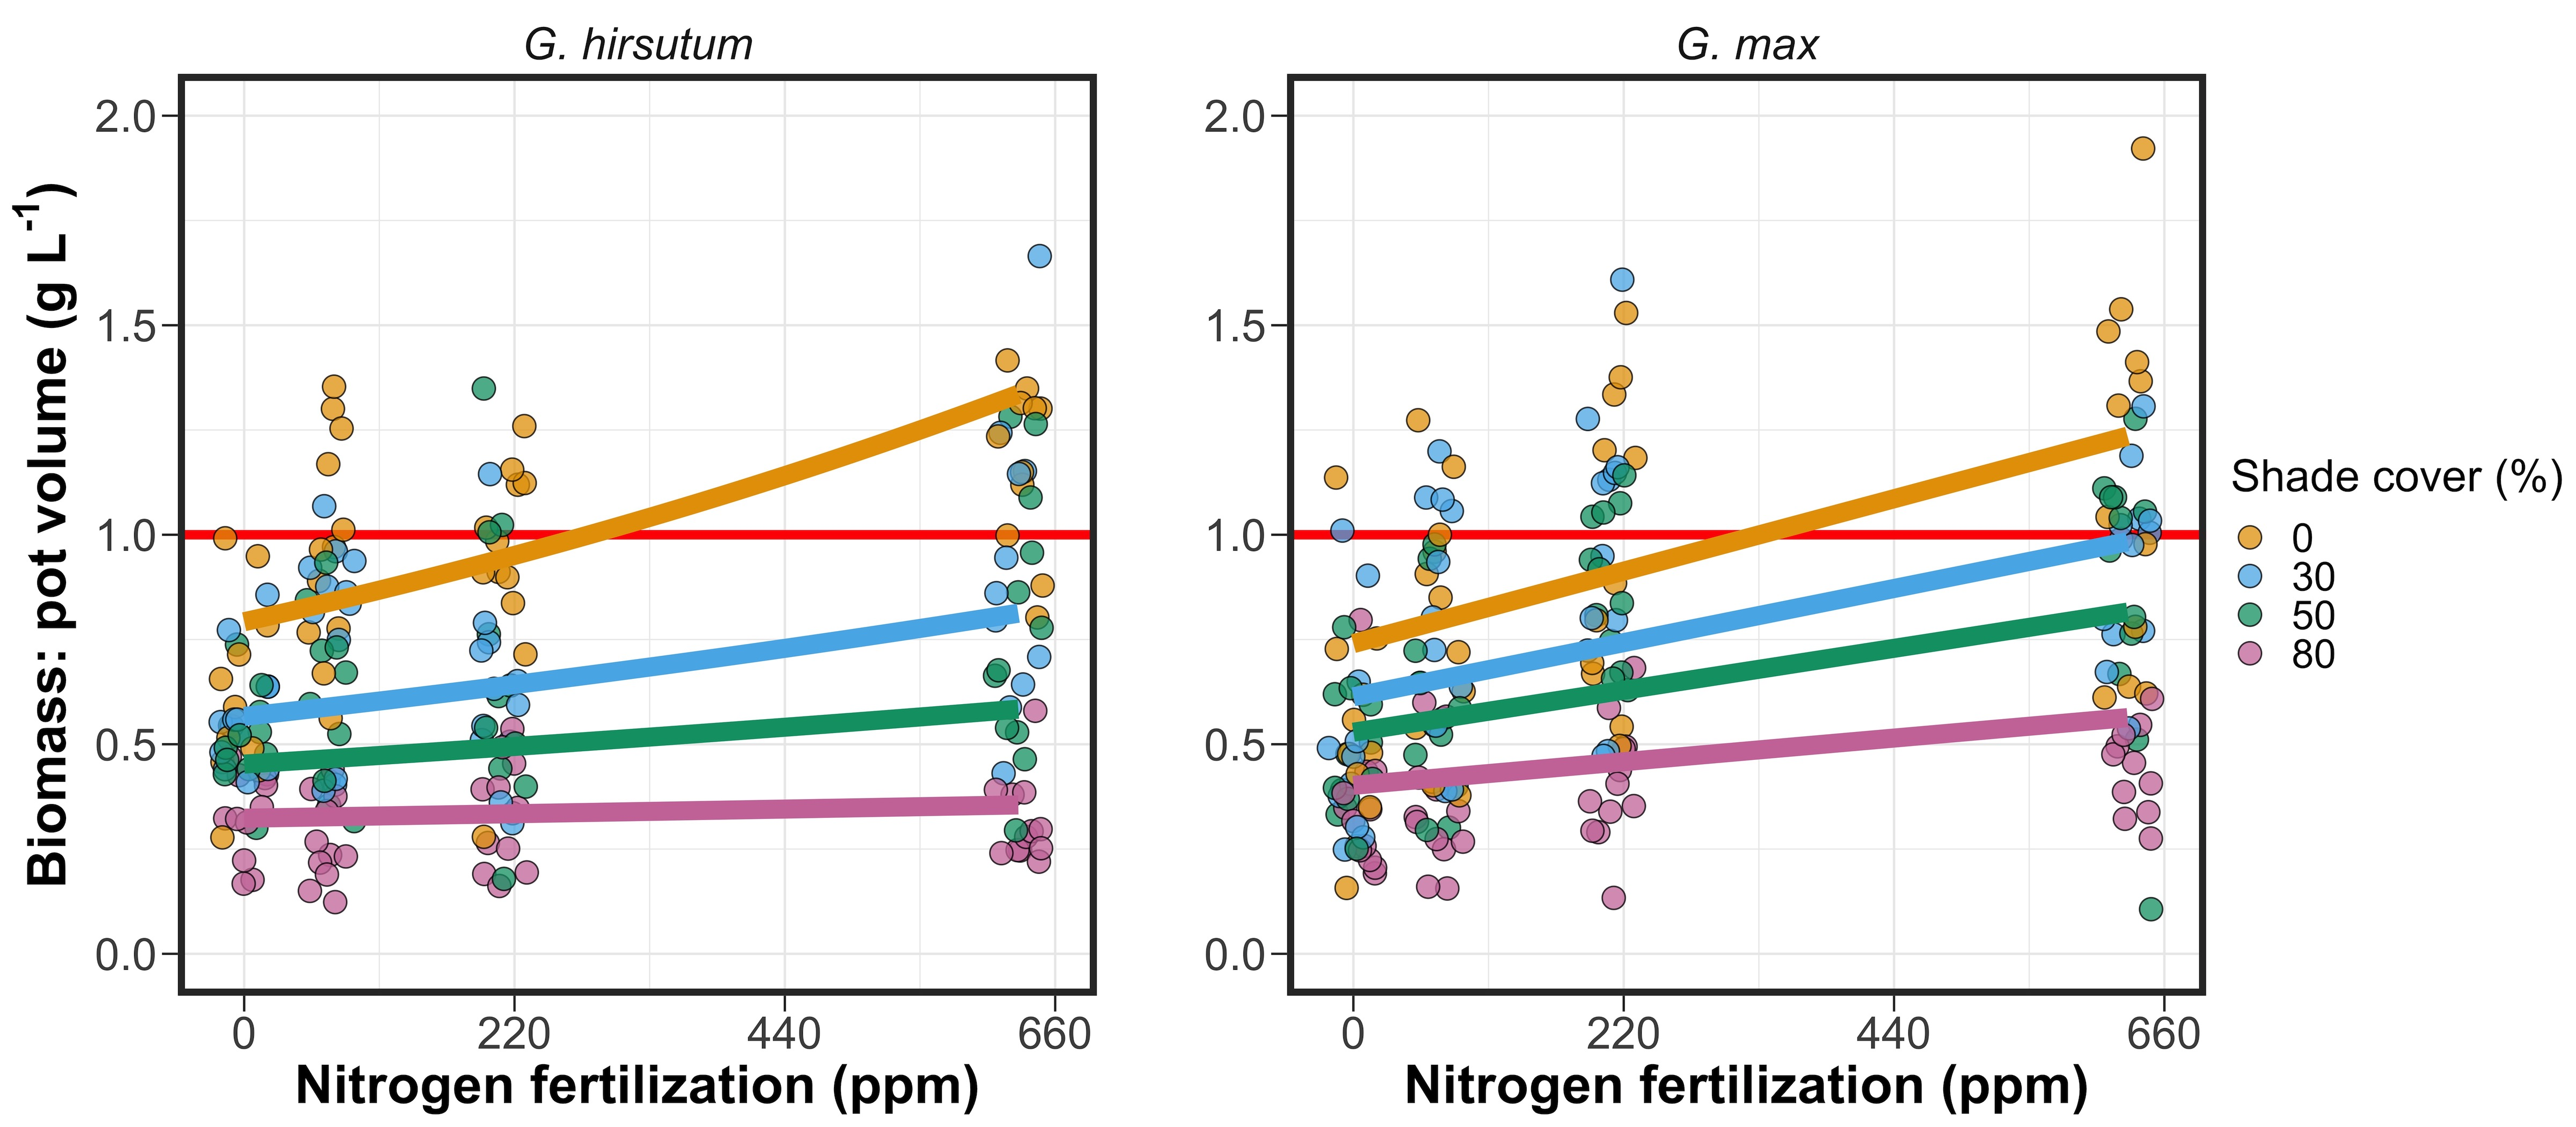
\includegraphics[width=\columnwidth]{ch2_LxN_Greenhouse/figs/figs1_bvr.jpg}
    \caption[Effects of shade cover and nitrogen fertilization on the ratio of plant biomass to rooting volume in \textit{G. hirsutum} and \textit{G. max}.]{Effects of shade cover and nitrogen fertilization on the ratio of plant biomass to rooting volume in \textit{G. hirsutum} (left panel) and \textit{G. max} (right panel). The red horizontal line indicates the recommended 1 g L$^{-1}$ threshold for biomass:pot volume recommended by \shortciteN{Poorter2012} to avoid pot size-induced growth limitation. Nitrogen fertilization treatments are represented on the x-axis. Shade cover treatments are represented through colored points and trendlines. Points are jittered for visibility. Yellow points and trendlines represent the 0\% shade cover treatment, blue points and trendlines represent the 30\% shade cover treatment, green points and trendlines represent the 50\% shade cover treatment, and purple points and trendlines represent the 80\% shade cover treatment. Solid trendlines indicate slopes that are significantly different from zero (Tukey: \textit{p}<0.05), while dashed trendlines indicate slopes that are not statistically different from zero.}
    \label{fig:figure.a1}
\end{figure}
\end{landscape}
\clearpage
\begin{singlespace}
    \chapter{\textbf{Appendix B: Supplemental material for "Soil nitrogen availability modifies leaf nitrogen economies in mature temperate deciduous forests: a direct test of photosynthetic least-cost theory"}}
\end{singlespace}

\setcounter{table}{0}
\renewcommand{\thetable}{B\arabic{table}}

\setcounter{figure}{0}
\renewcommand{\thefigure}{B\arabic{figure}}

\begin{table}[h!]
    \caption[Sample sizes of each species, abbreviated by their USDA NRCS PLANTS database code, within each plot at each site]{Sample sizes of each species, abbreviated by their USDA NRCS PLANTS database code, within each plot at each site$^*$}
    \label{table:tab.b1}
    \resizebox{\textwidth}{!}{%
    \begin{tabular}{p{0.5cm}p{2cm}|p{1cm}p{1cm}p{1cm}p{1cm}p{1cm}|p{1cm}}
        \hline
        \multicolumn{2}{l}{} &
        \multicolumn{1}{l}{ACRU} &
        \multicolumn{1}{l}{ACSA} &
        \multicolumn{1}{l}{FAGR} &
        \multicolumn{1}{l}{FRAM} &
        \multicolumn{1}{l}{QURU} &
        \multicolumn{1}{l}{$N_\mathrm{plot}$} \\
        \hline
        \multicolumn{2}{l}{Bald Hill} &
        &&&&&\\
                    & +N; +S                & 0  & 6  & 1  & 0  & 1  & 8  \\
                    & +N; $-$S              & 1  & 2  & 2  & 0  & 1  & 6  \\
                    & $-$N; +S              & 2  & 2  & 0  & 0  & 2  & 6  \\
                    & $-$N; $-$S            & 2  & 3  & 3  & 0  & 2  & 10 \\
        \multicolumn{2}{l}{Carter Creek}    &    &    &    &    &    &    \\
                    & +N; +S                & 0  & 6  & 1  & 2  & 0  & 9  \\
                    & +N; $-$S              & 0  & 4  & 0  & 2  & 0  & 6  \\
                    & $-$N; +S              & 0  & 5  & 1  & 4  & 0  & 10 \\
                    & $-$N; $-$S            & 0  & 7  & 0  & 0  & 0  & 7  \\
        \multicolumn{2}{l}{Mount Pleasant}  &    &    &    &    &    &    \\
                    & +N; +S                & 3  & 2  & 1  & 0  & 3  & 9  \\
                    & +N; $-$S              & 0  & 5  & 4  & 1  & 0  & 10 \\
                    & $-$N; +S              & 1  & 2  & 4  & 0  & 0  & 7  \\
                    & $-$N; $-$S            & 3  & 3  & 1  & 2  & 1  & 10 \\
      \hline
      \multicolumn{2}{l}{$N_\mathrm{spp}$}  & 12 & 47 & 18 & 11 & 10 & 98
      \end{tabular}%
      }
      \end{table}
      \begin{singlespace}
        \noindent $^*$Plots within each site are represented based on nitrogen and sulfur addition status. The final column on the right depicts total sample size per plot in each site ($N_\mathrm{plot}$) and the final row on the bottom represents cumulative species sample size across all plots and all sites ($N_\mathrm{spp}$). Key: ACRU=\textit{A. rubrum}; ACSA=\textit{A. saccharum}; FAGR=\textit{F. grandifolia}; FRAM=\textit{F. americana}; QURU=\textit{Q. rubra}
      \end{singlespace}
    \clearpage

    \newpage
    \begin{table}[]
        \caption[Analysis of variance results exploring the linear effect of leaf temperature on net photosynthesis rate and stomatal conductance measured at 400 $\mu \mathrm{mol\ mol^{-1}\ CO_2}$]{Analysis of variance results exploring the linear effect of leaf temperature on net photosynthesis rate ($A_\mathrm{net}$; $\mathrm{\mu mol\ m^{-2}\ s^{-1}}$) and stomatal conductance ($g_\mathrm{sw}$; $\mathrm{\mu mol\ m^{-2}\ s^{-1}}$) measured at 400 $\mu \mathrm{mol\ mol^{-1}\ CO_2}$}
        \centering
        \label{table:tab.b2}
        %\resizebox{\textwidth}{!}{%
        \begin{tabular}{p{4cm}p{0.5cm}p{3cm}p{3m}p{3cm}p{3cm}}
            && \multicolumn{2}{r}{$A_\mathrm{net}$} & \multicolumn{2}{r}{$g_\mathrm{sw}$} \\
            \hline
            & df                    
            & \multicolumn{1}{r}{$\chi^2$}      & \multicolumn{1}{r}{\textit{p}}
            & \multicolumn{1}{r}{$\chi^2$}      & \multicolumn{1}{r}{\textit{p}}
            \\
            \hline
            
            Leaf temperature & 1    
            & \multicolumn{1}{r}{1.287}         & \multicolumn{1}{r}{0.257}      
            & \multicolumn{1}{r}{1.716}         & \multicolumn{1}{r}{0.190} \\

\end{tabular}%
%}
\end{table}
\begin{singlespace}
\noindent $^*$Results detail linear mixed effects model where temperature was regressed against net photosynthesis or stomatal conductance, with site and species designated as random intercept terms. Significance was determined using Type II Wald $\chi^2$ tests ($\alpha$=0.05).
\end{singlespace}
\clearpage

\newpage
\begin{table}[]
    \centering
    \caption[Second order log-polynomial regression coefficients that described the effect of leaf temperature on net photosynthesis and stomatal conductance measured at 400 $\mu \mathrm{mol\ mol^{-1}\ CO_2}$]{Second order log-polynomial regression coefficients that described the effect of leaf temperature on net photosynthesis ($A_\mathrm{net}$; $\mathrm{\mu mol\ m^{-2}\ s^{-1}}$) and stomatal conductance ($g_\mathrm{sw}$; $\mathrm{\mu mol\ m^{-2}\ s^{-1}}$) measured at 400 $\mu \mathrm{mol\ mol^{-1}\ CO_2}^*$}
    \label{table:tab.b3}
    %\resizebox{\textwidth}{!}
\end{table}
\begin{singlespace}
    \noindent $^*$Net photosynthesis and stomatal conductance values were fit to the log polynomial equation $\mathrm{log}(y)= a + bx + cx^2$, where $x$ is leaf temperature in \textdegree{}C.
\end{singlespace}
\clearpage

\newpage
\begin{landscape}
\begin{table}[]
    \caption[Mean, standard error, and 95\% confidence interval ranges of soil nitrogen availability estimates across all measured plots]{Mean, standard error, and 95\% confidence interval ranges of soil nitrogen availability estimates across all measured plots. All units are expressed as $\mu \mathrm{g\ N\ g^{-1}\ resin\ d^{-1}}$}
    \centering
    \label{tab:table.b4}
    %\resizebox{\columnwidth}{!}{%
    \begin{tabular}{p{3cm}p{3.5cm}p{1.5cm}p{1.5cm}p{2.75cm}p{2.75cm}}
        \hline
        Site           & Treatment        & \multicolumn{1}{r}{Mean }   & \multicolumn{1}{r}{SE}    & \multicolumn{1}{r}{Lower 95\% CI} & \multicolumn{1}{r}{Upper 95\% CI} \\
        \hline
        Bald Hill      & Ammonium sulfate & \multicolumn{1}{r}{27.11}   & \multicolumn{1}{r}{6.14}  & \multicolumn{1}{r}{15.08}         & \multicolumn{1}{r}{39.13}  \\
        Bald Hill      & Control          & \multicolumn{1}{r}{14.41}   & \multicolumn{1}{r}{5.02}  & \multicolumn{1}{r}{4.56}          & \multicolumn{1}{r}{24.26}  \\
        Bald Hill      & Sodium nitrate   & \multicolumn{1}{r}{20.65}   & \multicolumn{1}{r}{3.15}  & \multicolumn{1}{r}{14.46}         & \multicolumn{1}{r}{26.83}  \\
        Bald Hill      & Sulfur           & \multicolumn{1}{r}{6.33}    & \multicolumn{1}{r}{2.19}  & \multicolumn{1}{r}{2.04}          & \multicolumn{1}{r}{10.62}  \\
        Carter Creek   & Ammonium sulfate & \multicolumn{1}{r}{26.94}   & \multicolumn{1}{r}{5.36}  & \multicolumn{1}{r}{16.43}         & \multicolumn{1}{r}{37.44}  \\
        Carter Creek   & Control          & \multicolumn{1}{r}{19.87}   & \multicolumn{1}{r}{1.92}  & \multicolumn{1}{r}{16.10}         & \multicolumn{1}{r}{23.64}  \\
        Carter Creek   & Sodium nitrate   & \multicolumn{1}{r}{15.51}   & \multicolumn{1}{r}{4.16}  & \multicolumn{1}{r}{7.36}          & \multicolumn{1}{r}{23.65}  \\
        Carter Creek   & Sulfur           & \multicolumn{1}{r}{5.50}    & \multicolumn{1}{r}{1.40}  & \multicolumn{1}{r}{2.75}          & \multicolumn{1}{r}{8.25}   \\
        Mount Pleasant & Ammonium sulfate & \multicolumn{1}{r}{8.02}    & \multicolumn{1}{r}{2.31}  & \multicolumn{1}{r}{3.49}          & \multicolumn{1}{r}{12.56}  \\
        Mount Pleasant & Control          & \multicolumn{1}{r}{2.00}    & \multicolumn{1}{r}{0.57}  & \multicolumn{1}{r}{0.89}          & \multicolumn{1}{r}{3.11}   \\
        Mount Pleasant & Sodium nitrate   & \multicolumn{1}{r}{2.52}    & \multicolumn{1}{r}{0.68}  & \multicolumn{1}{r}{1.19}          & \multicolumn{1}{r}{3.85}   \\
        Mount Pleasant & Sulfur           & \multicolumn{1}{r}{2.42}    & \multicolumn{1}{r}{0.39}  & \multicolumn{1}{r}{1.66}          & \multicolumn{1}{r}{3.17} \\
        \hline        
    \end{tabular}%}
    \end{table}
\end{landscape}
\clearpage

\newpage
\begin{landscape}
    \begin{figure}
        \centering
        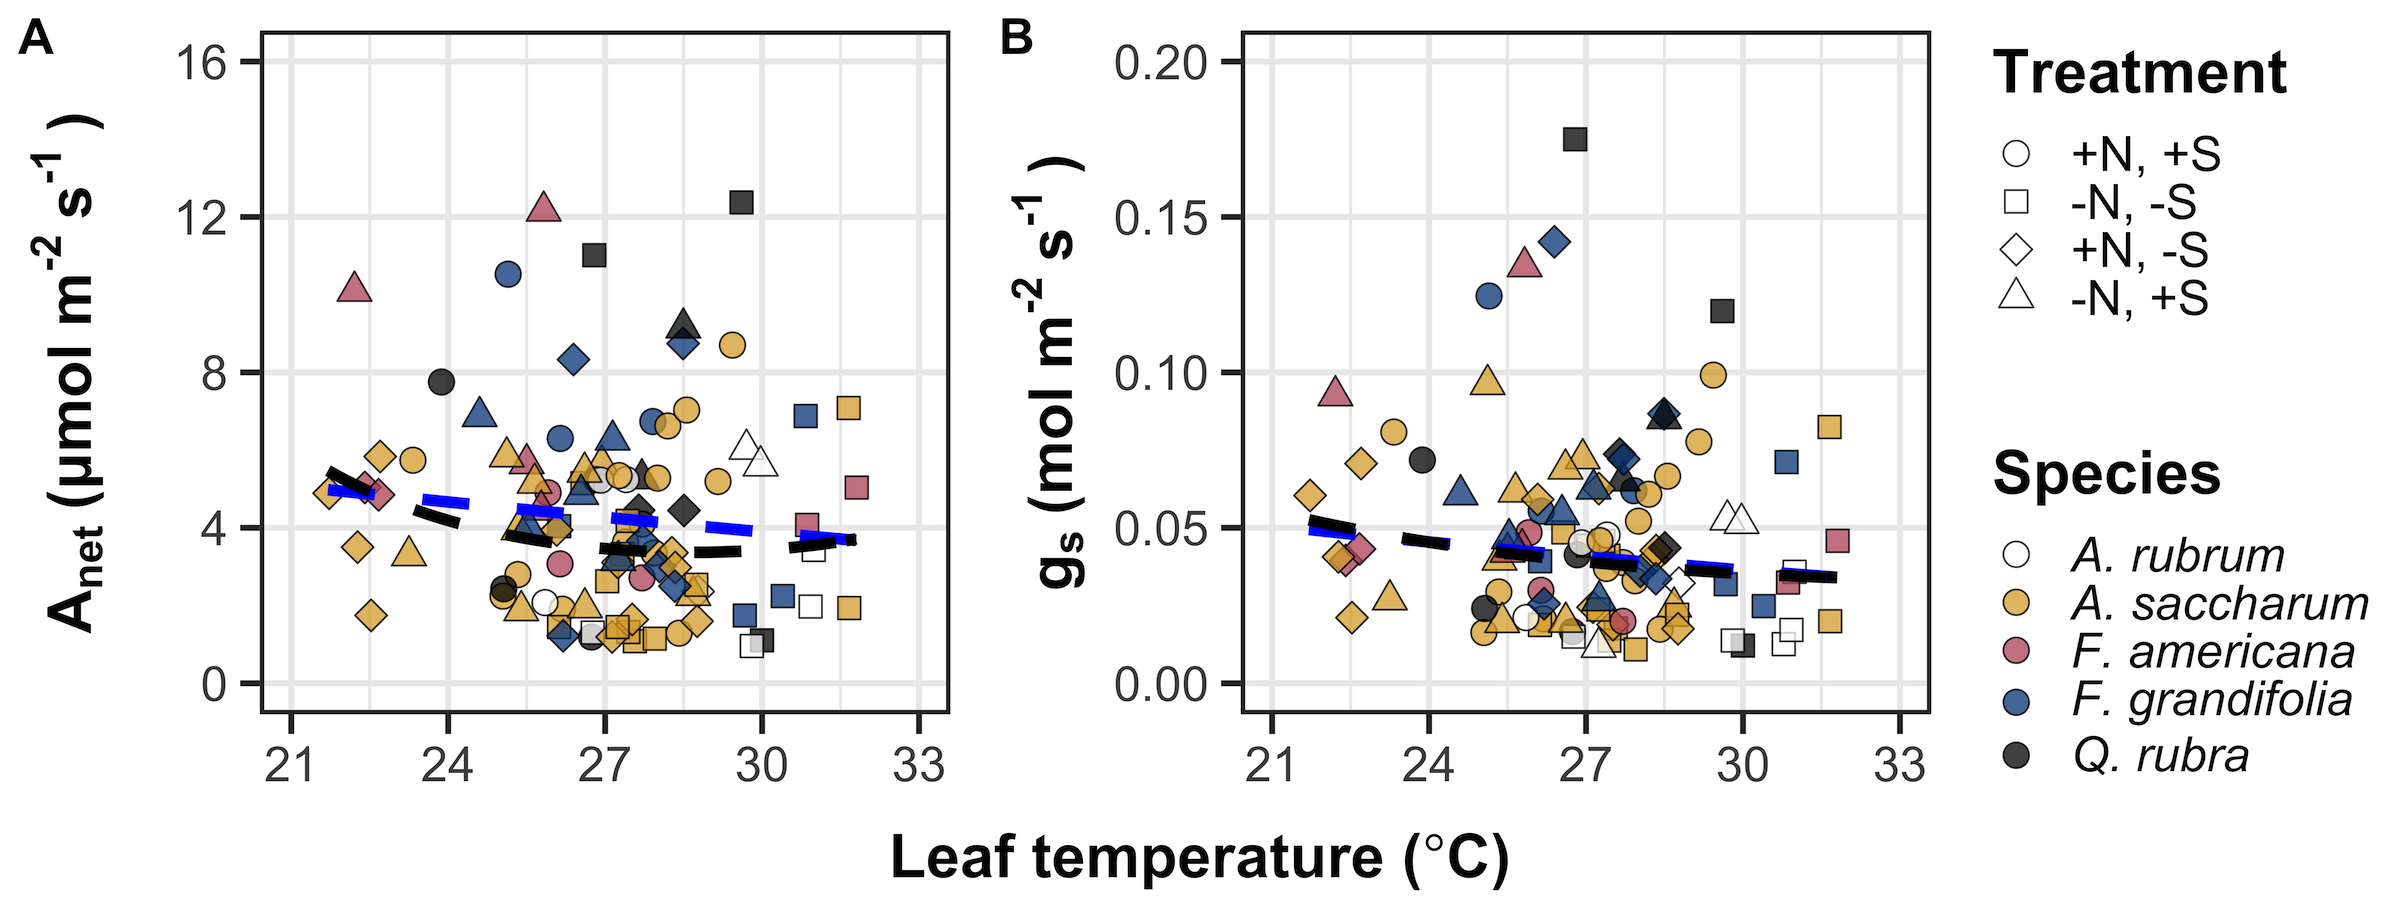
\includegraphics[width=\columnwidth]{ch3_NxpH/figs/NxS_figS1_leaftemp.jpg}
        \caption[Effects of leaf temperature on net photosynthesis rate and stomatal conductance values when measured at 400 $\mu \mathrm{mol\ mol^{-1}\ CO_2}$]{Effects of leaf temperature on net photosynthesis rate (A) and stomatal conductance (B) values when measured at 400 $\mu \mathrm{mol\ mol^{-1}\ CO_2}$. Leaf temperature is represented on the x-axis, while species are represented as colored points. Colored points and shapes are as explained in Figure \ref{fig:figure3.1}. The dashed blue trendline describes the linear relationship between leaf temperature and each response variable, while the dashed black trendline describes the same relationship with a log-polynomial regression equation.}
        \label{fig:figure.b1}
    \end{figure}
\end{landscape}
\clearpage

\begin{singlespace}
    \chapter{\textbf{Appendix C: Supplemental material for "The relative cost of resource use for photosynthesis drives variance in leaf nitrogen content across a climate and soil resource availability gradient"}}
\end{singlespace}

\setcounter{table}{0}
\renewcommand{\thetable}{C\arabic{table}}

\setcounter{figure}{0}
\renewcommand{\thefigure}{C\arabic{figure}}


\section*{C.1 Calculations for soil water holding capacity}\label{appendix.c1}
\noindent Water holding capacity ($\theta_\mathrm{WHC}$; mm) was calculated as a function of the volumetric soil water storage at field capacity ($W_\mathrm{FC}$; $\mathrm{m^3\ m^{-3}}$), and the volumetric soil water storage at wilting point ($W_\mathrm{PWP}$; $\mathrm{m^3\ m^{-3}}$):

\begin{equation}
    \label{eqn_s4.1} \tag{C4.1}
    \theta_{WHC} = (W_{FC}-W_{PWP})(1-f_{gravel}) * min(z_{bedrock}, z_{max})
\end{equation}

\noindent where $f_\mathrm{gravel}$ (\%) is the fraction of gravel content in soil, $z_\mathrm{bedrock}$ (mm) is the distance to bedrock, and $z_\mathrm{max}$ (mm) is the maximum allowable distance to bedrock, set to 2000mm. $W_\mathrm{FC}$ is calculated as:

\begin{equation}
    \label{eqn_s4.2} \tag{C4.2}
    \theta_{FC} = k_{fc}+(1.283*(k_{fc})^2-0.374*k_{fc}-0.015)
\end{equation}

\noindent where

\begin{equation}
    \label{eqn_s4.3} \tag{C4.3}
    \begin{aligned}
        k_{fc}= -0.251 * f_{sand} + 0.195 * f_{clay} + 0.011 * f_{OM} \\ + 0.006 * (f_{sand} * f_{OM}) - 0.027 * (f_{clay} \\ * f_{OM}) + 0.452 * (f_{sand} * f_{clay}) + 0.299
    \end{aligned}	
\end{equation}

\noindent $W_\mathrm{PWP}$ is calculated as:

\begin{equation}
    \label{eqn_s4.4} \tag{C4.4}
    W_{PWP}=k_{pwp}+(0.14*k_{pwp}-0.02)	
\end{equation}

\noindent where

\begin{equation}
    \label{eqn_s4.5} \tag{C4.5}
    \begin{aligned}
        k_{pwp} = -0.024 * f_{sand} + 0.487 * f_{clay} + 0.006 * f_{OM} \\ + 0.005 * (f_{sand} * f_{OM}) - 0.013 * (f_{clay} \\ * f_{OM}) + 0.068 * (f_{sand} * f_{clay}) + 0.031
    \end{aligned}
\end{equation}

\noindent In Equations \ref{eqn_s4.4} and \ref{eqn_s4.5}, $f_\mathrm{sand}$ (\%) is the fraction of sand content in soil (\%), $f_\mathrm{clay}$ (\%) is the fraction of clay content in soil (\%), and $f_\mathrm{OM}$ is the fraction of organic matter in soil (\%). Organic matter in the soil was calculated by converting soil organic carbon data extracted from SoilGrids 2.0 to soil organic matter using the van Bemmelen factor (1.724 conversion factor).
\clearpage


\begin{landscape}
    \begin{table}[]
        \caption{List of sampled species and their plant functional group assignment}
        \label{tab:tab.c1}
        \resizebox{\columnwidth}{!}{%
            \begin{tabular}{p{2cm}p{5cm}p{2cm}p{2cm}p{2cm}p{2cm}p{3.5cm}p{2cm}}
            \hline
            \textbf{Symbol} & \textbf{Species} & \textbf{\begin{tabular}[c]{@{}l@{}}Photo.\\ pathway\end{tabular}} &
            \textbf{\begin{tabular}[c]{@{}l@{}}Growth\\ duration\end{tabular}} & \textbf{Growth  habit} &
            \textbf{N-fixer?} & \textbf{\begin{tabular}[c]{@{}l@{}}Plant functional \\ group\end{tabular}} &
            \multicolumn{1}{l}{\textbf{\begin{tabular}[c]{@{}l@{}}Number \\ sampled\end{tabular}}} \\
            \hline
            ACAN11 & \textit{Acaciella angustissima}    & c3 & perennial & forb           & yes & c3\_legume    & 3  \\
            AMAR2  & \textit{Ambrosia artemisiifolia}   & c3 & annual    & forb           & no  & c3\_nonlegume & 25 \\
            AMPS   & \textit{Ambrosia psilostachya}     & c3 & perennial & forb           & no  & c3\_nonlegume & 32 \\
            ARAL3  & \textit{Argemone albiflora}        & c3 & annual    & forb           & no  & c3\_nonlegume & 3  \\
            ARPU9  & \textit{Aristida purpurea}         & c4 & perennial & graminoid      & no  & c4\_nonlegume & 2  \\
            ASAS   & \textit{Asclepias asperula}        & c3 & perennial & forb           & no  & c3\_nonlegume & 3  \\
            ASLA4  & \textit{Asclepias latifolia}       & c3 & perennial & forb           & no  & c3\_nonlegume & 3  \\
            ASSY   & \textit{Asclepias syriaca}         & c3 & perennial & forb           & no  & c3\_nonlegume & 18 \\
            BOIS   & \textit{Bothriochloa ischaemum}    & c4 & perennial & graminoid      & no  & c4\_nonlegume & 6  \\
            BOSA   & \textit{Bothriochloa saccharoides} & c4 & perennial & graminoid      & no  & c4\_nonlegume & 6  \\
            CAPL3  & \textit{Carex planostachys}        & c4 & perennial & graminoid      & no  & c4\_nonlegume & 3  \\
            CAREX  & \textit{Carex} spp.                & c4 & perennial & graminoid      & no  & c4\_nonlegume & 16 \\
            CHFE3  & \textit{Chamaesyce fendleri}       & c3 & perennial & forb           & no  & c3\_nonlegume & 2  \\
            CHPI8  & \textit{Chyrysopsis pilosa}        & c3 & annual    & forb           & no  & c3\_nonlegume & 3  \\
            COCO13 & \textit{Conoclinium coelestinum}   & c3 & perennial & forb           & no  & c3\_nonlegume & 3  \\
            COER   & \textit{Commelina erecta}          & c3 & perennial & forb           & no  & c3\_nonlegume & 3  \\
            CRGLL  & \textit{Croton glandulosus}        & c3 & annual    & forb           & no  & c3\_nonlegume & 22 \\
            CYDA   & \textit{Cynodon dactylon}          & c4 & perennial & graminoid      & no  & c4\_nonlegume & 15 \\
            DIAN   & \textit{Dichanthium annulatum}     & c4 & perennial & graminoid      & no  & c4\_nonlegume & 8  \\
            ENPE4  & \textit{Engelmannia peristenia}    & c3 & perennial & forb           & no  & c3\_nonlegume & 6  \\
            EUMA8  & \textit{Euphorbia marginata}       & c3 & annual    & forb           & no  & c3\_nonlegume & 6  \\
            GAPU   & \textit{Gaillardia pulchella}      & c3 & annual    & forb           & no  & c3\_nonlegume & 16 \\
            GLGO   & \textit{Glandularia gooddingii}    & c3 & perennial & forb           & no  & c3\_nonlegume & 2  \\
            HEAN3  & \textit{Helianthus annuus}         & c3 & annual    & forb           & no  & c3\_nonlegume & 6  \\
            \hline
        \end{tabular}}
    \end{table}
\end{landscape}
\clearpage

\newpage
\begin{landscape}
    \begin{table}[]
        \caption{List of sampled species and their plant functional group assignment (cont.)}
        \label{tab:tab.c2}
        \resizebox{\columnwidth}{!}{%
            \begin{tabular}{p{2cm}p{5cm}p{2cm}p{2cm}p{2cm}p{2cm}p{3.5cm}p{2cm}}
        \hline
        \textbf{Symbol} & \textbf{Species} & \textbf{\begin{tabular}[c]{@{}l@{}}Photo.\\ pathway\end{tabular}} &
        \textbf{\begin{tabular}[c]{@{}l@{}}Growth\\ duration\end{tabular}} & \textbf{Growth habit} &
        \textbf{N-fixer?} & \textbf{\begin{tabular}[c]{@{}l@{}}Plant functional \\ group\end{tabular}} &
        \multicolumn{1}{l}{\textbf{\begin{tabular}[c]{@{}l@{}}Number \\ sampled\end{tabular}}} \\
        \hline
        HECA8  & \textit{Heterotheca canescens}     & c3 & perennial & forb           & no  & c3\_nonlegume & 2  \\
        HETE3  & \textit{Heliotropium tenellum}     & c3 & annual    & forb           & no  & c3\_nonlegume & 3  \\
        IVAX   & \textit{Iva axillaris}             & c3 & perennial & forb           & no  & c3\_nonlegume & 4  \\
        LIAT   & \textit{Lilaeopsis attenuata}      & c3 & perennial & forb           & no  & c3\_nonlegume & 3  \\
        LIPU   & \textit{Liatris punctata}          & c3 & perennial & forb           & no  & c3\_nonlegume & 3  \\
        LOPE   & \textit{Lolium perenne}            & c3 & perennial & graminoid      & no  & c3\_nonlegume & 9  \\
        MIQU2  & \textit{Mimosa quadrivalvis}       & c3 & perennial & forb           & yes & c3\_legume    & 15 \\
        NALE3  & \textit{Nassella leucotricha}      & c3 & perennial & graminoid      & no  & c3\_nonlegume & 19 \\
        OECU2  & \textit{Oenothera curtiflora}      & c3 & annual    & forb           & no  & c3\_nonlegume & 3  \\
        OENOT  & \textit{Oenothera} spp.            & c3 & annual    & forb           & no  & c3\_nonlegume & 1  \\
        PAVI2  & \textit{Panicum virgatum}          & c4 & perennial & graminoid      & no  & c4\_nonlegume & 12 \\
        RACO3  & \textit{Ratibida columnifera}      & c3 & perennial & forb           & no  & c3\_nonlegume & 40 \\
        RHSET  & \textit{Rhynchosia senna}          & c3 & perennial & forb           & yes & c3\_legume    & 1  \\
        RUHI2  & \textit{Rudbeckia hirta}           & c3 & perennial & forb           & no  & c3\_nonlegume & 3  \\
        RUNU   & \textit{Ruellia nudiflora}         & c3 & perennial & forb           & no  & c3\_nonlegume & 15 \\
        RUTR   & \textit{Rubus trivialis}           & c3 & perennial & vine           & no  & c3\_nonlegume & 3  \\
        SAFA2  & \textit{Salvia farinacea}          & c3 & perennial & forb           & no  & c3\_nonlegume & 7  \\
        SCHIZ4 & \textit{Schizachyrium} spp.        & c4 & perennial & graminoid      & no  & c4\_nonlegume & 8  \\
        SCSC   & \textit{Schizachyrium scoparium}   & c4 & perennial & graminoid      & no  & c4\_nonlegume & 3  \\
        SODI   & \textit{Solanum dimidiatum}        & c3 & perennial & forb           & no  & c3\_nonlegume & 1  \\
        SOEL   & \textit{Solanum elaeagnifolium}    & c3 & perennial & forb           & no  & c3\_nonlegume & 53 \\
        SOHA   & \textit{Sorghum halapense}         & c4 & perennial & graminoid      & no  & c4\_nonlegume & 38 \\
        STTE3  & \textit{Stillingia texana}         & c3 & perennial & forb           & no  & c3\_nonlegume & 3  \\
        VEOC   & \textit{Verbesina occidentalis}    & c3 & perennial & forb           & no  & c3\_nonlegume & 3  \\
        VEST   & \textit{Verbena stricta}           & c3 & perennial & forb           & no  & c3\_nonlegume & 3  \\
        \hline
    \end{tabular}}
\end{table}
\end{landscape}
\clearpage

\newpage
\begin{table}
    \centering
    \caption[Model selection results for soil moisture and vapor pressure deficit]{Model selection results for soil moisture and vapor pressure deficit. Soil moisture was used in a bivariate regression against log-transformed $\beta$, while vapor pressure deficit was used in bivariate regressions against leaf $C_\mathrm{i}$:$C_\mathrm{a}$}
    \label{tab:tab.c4}
    %\resizebox{\columnwidth}{!}{%
        \begin{tabular}{p{2cm}p{2cm}p{2cm}p{2cm}p{2cm}}
            & \multicolumn{2}{l}{Soil moisture} & \multicolumn{2}{l}{VPD} \\
            \hline
            Day & AICc             & RMSE           & AICc              & RMSE      \\
            \hline
            1   & 1431.77          & 0.8400         & -772.71           & 0.0853    \\
            2   & 1431.76          & 0.8400         & -775.47           & 0.0849    \\
            3   & 1431.78          & 0.8400         & -770.86           & 0.0854    \\
            4   & 1431.79          & 0.8401         & \textbf{-793.49}  & \textbf{0.0839}    \\
            5   & 1431.79          & 0.8401         & -771.66           & 0.0853    \\
            6   & 1431.78          & 0.8401         & -771.66           & 0.0853    \\
            7   & 1431.78          & 0.8401         & -771.05           & 0.0854    \\
            8   & 1431.76          & 0.8401         & -770.94           & 0.0854    \\
            9   & 1431.75          & 0.8401         & -770.11           & 0.0854    \\
            10  & 1431.74          & 0.8401         & -770.08           & 0.0855    \\
            15  & 1431.54          & 0.8401         & -768.64           & 0.0856    \\
            20  & 1431.40          & 0.8401         & -769.77           & 0.0855    \\
            30  & 1431.23          & 0.8400         & -772.18           & 0.0853    \\
            60  & 1429.84          & 0.8391         & -779.06           & 0.0848    \\
            90  & \textbf{1429.14} & \textbf{0.8385}& -773.99           & 0.0852    \\
            \hline
\end{tabular}
%}
\end{table}
\clearpage

\newpage
\begin{landscape}
    \begin{figure}
        \centering
        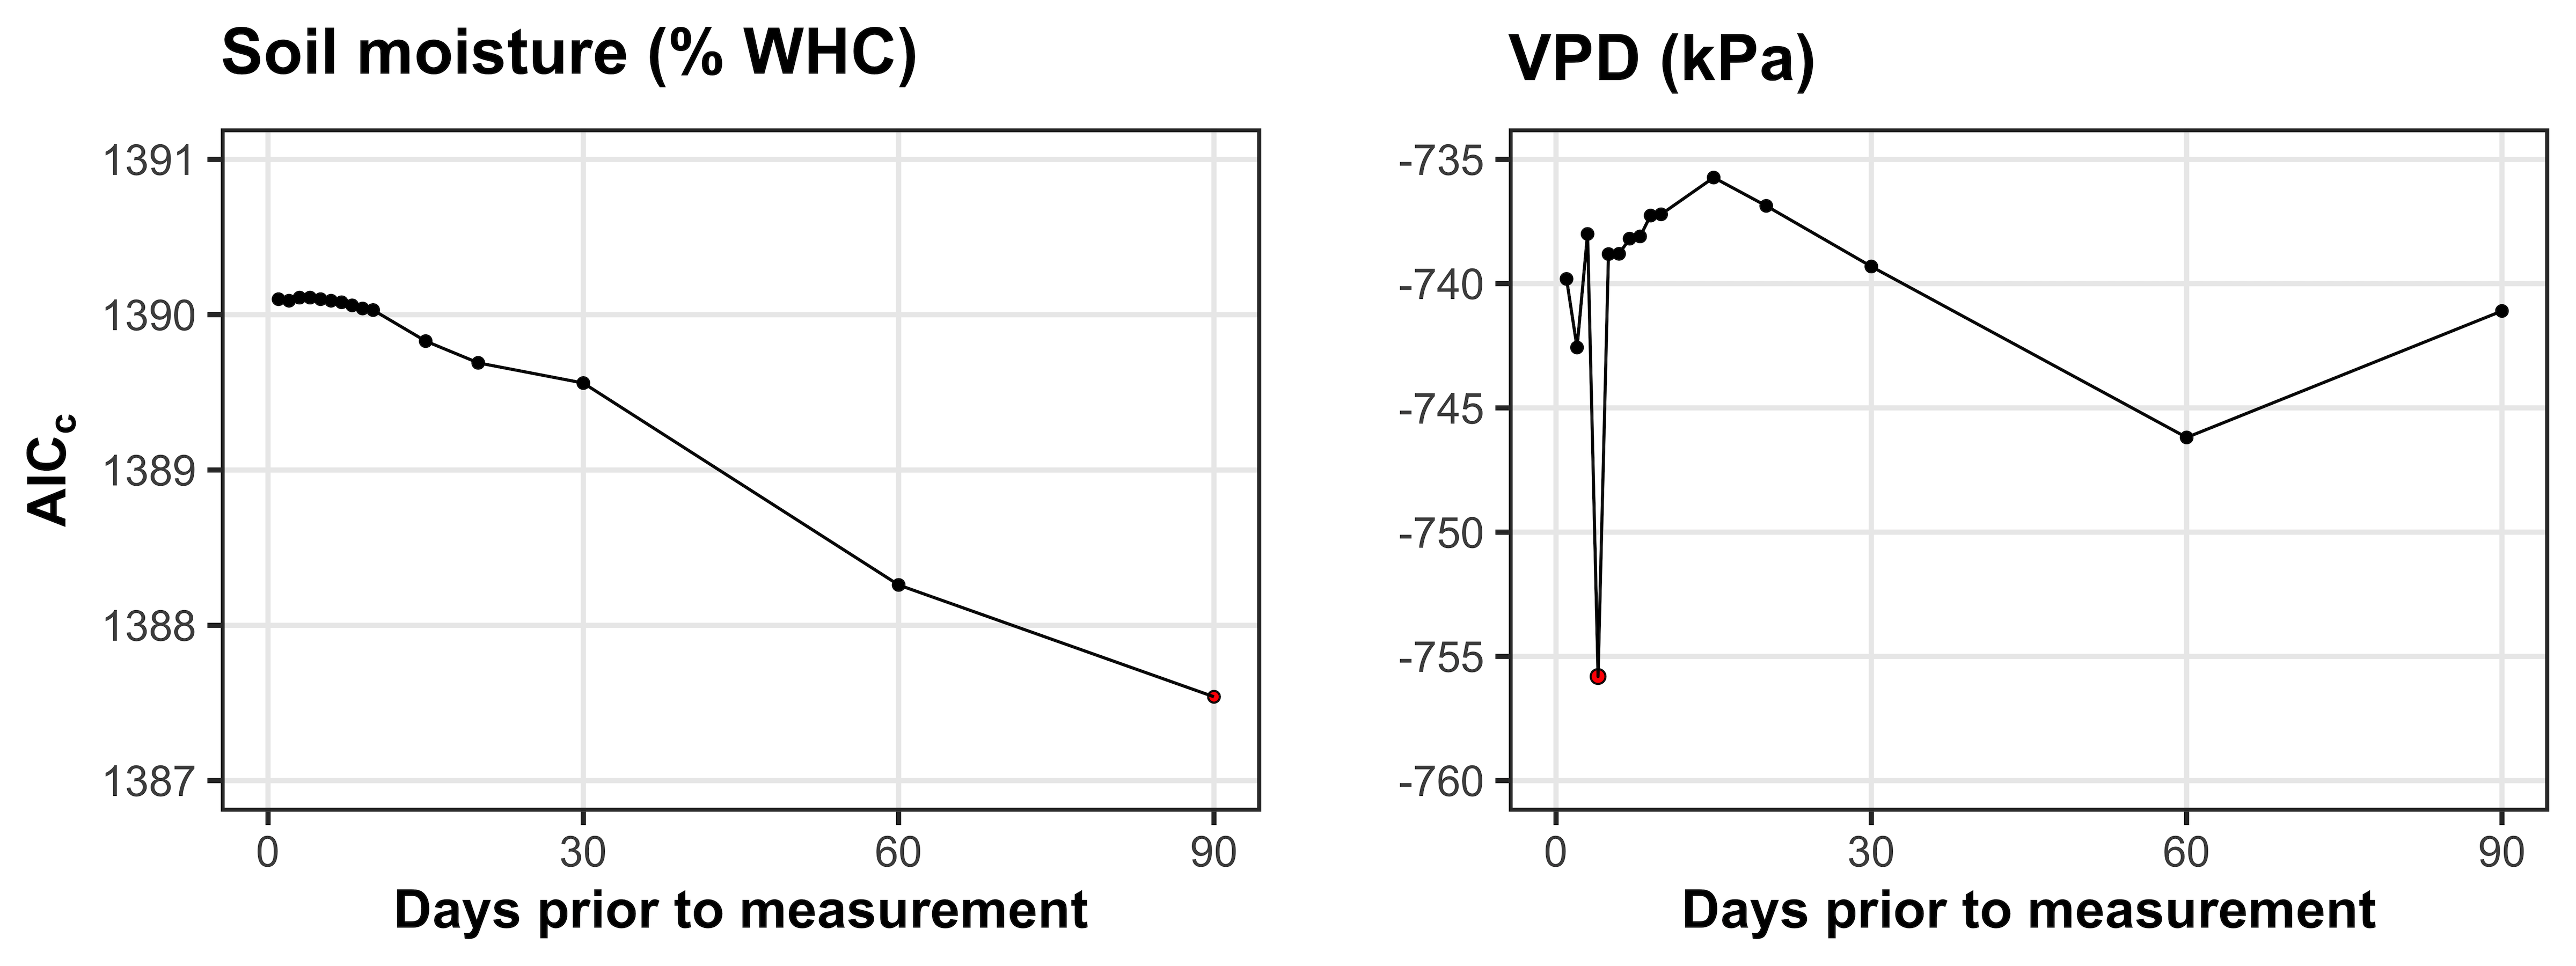
\includegraphics[width=\linewidth]{ch4_TXeco/figs/TXeco_figS2_aicc.png}
        \caption[Model selection results exploring relevant timescales for soil moisture and vapor pressure deficit]{Model selection results exploring relevant timescales for soil moisture (left panel) and vapor pressure deficit (right panel). The x-axis indicates the number of days before each site visit and the y-axis notes the corrected Akaike Information Criterion value. The timescale with the lowest AICc value, and therefore most relevant timescale to include in statistical models, is noted as a red point.}
        \label{fig:figure.c1}
    \end{figure}
\end{landscape}
\clearpage


\begin{singlespace}
    \chapter{\textbf{Appendix D: Supplemental material for "Optimal resource investment to photosynthetic capacity maximizes nutrient allocation to whole plant growth under elevated CO$_2$"}}
\end{singlespace}

\setcounter{table}{0}
\renewcommand{\thetable}{D\arabic{table}}
\setcounter{figure}{0}
\renewcommand{\thefigure}{D\arabic{figure}}

\begin{table}[!h]
    \caption{Summary table containing volumes of compounds used to create modified Hoagland’s solutions for each soil nitrogen fertilization treatment. All volumes are expressed as milliliters per liter (mL/L)}
    \label{table:tab.d1}
    \resizebox{\columnwidth}{!}{
    \begin{tabular}{p{4cm}p{2cm}p{2cm}p{2cm}p{2cm}p{2cm}}
        \hline
        \textbf{Compound}
        & \multicolumn{1}{r}{\textbf{0 ppm N}}
        & \multicolumn{1}{r}{\textbf{35 ppm N}}
        & \multicolumn{1}{r}{\textbf{70 ppm N}}
        & \multicolumn{1}{r}{\textbf{105 ppm N}}
        & \multicolumn{1}{r}{\textbf{140 ppm N}} \\
        \hline
        1 M NH$_4$H$_2$PO$_4$   & \multicolumn{1}{r}{0}         & \multicolumn{1}{r}{0.165}     & \multicolumn{1}{r}{0.33}      & \multicolumn{1}{r}{0.5}       & \multicolumn{1}{r}{0.67} \\
        2 M KNO$_3$             & \multicolumn{1}{r}{0}         & \multicolumn{1}{r}{0.335}     & \multicolumn{1}{r}{0.67}      & \multicolumn{1}{r}{1}         & \multicolumn{1}{r}{1.33} \\
        2 M Ca(NO$_3$)$_2$      & \multicolumn{1}{r}{0}         & \multicolumn{1}{r}{0.335}     & \multicolumn{1}{r}{0.67}      & \multicolumn{1}{r}{1}         & \multicolumn{1}{r}{1.33} \\
        1 M NH$_4$NO$_3$        & \multicolumn{1}{r}{0}         & \multicolumn{1}{r}{0.165}     & \multicolumn{1}{r}{0.33}      & \multicolumn{1}{r}{0.5}       & \multicolumn{1}{r}{0.67} \\
        8 M NH$_4$NO$_3$        & \multicolumn{1}{r}{0}         & \multicolumn{1}{r}{0}         & \multicolumn{1}{r}{0}         & \multicolumn{1}{r}{0}         & \multicolumn{1}{r}{0}    \\
        1 M KH$_2$PO$_4$        & \multicolumn{1}{r}{1}         & \multicolumn{1}{r}{0.85}      & \multicolumn{1}{r}{0.67}      & \multicolumn{1}{r}{0.5}       & \multicolumn{1}{r}{0.33} \\
        1 M KCl                 & \multicolumn{1}{r}{3}         & \multicolumn{1}{r}{2.45}      & \multicolumn{1}{r}{2}         & \multicolumn{1}{r}{1.5}       & \multicolumn{1}{r}{1}    \\
        1 M CaCO$_3$            & \multicolumn{1}{r}{4}         & \multicolumn{1}{r}{3.33}      & \multicolumn{1}{r}{2.67}      & \multicolumn{1}{r}{2}         & \multicolumn{1}{r}{1.33} \\
        2 M MgSO$_4$            & \multicolumn{1}{r}{1}         & \multicolumn{1}{r}{1}         & \multicolumn{1}{r}{1}         & \multicolumn{1}{r}{1}         & \multicolumn{1}{r}{1}    \\
        10\% Fe-EDTA            & \multicolumn{1}{r}{1}         & \multicolumn{1}{r}{1}         & \multicolumn{1}{r}{1}         & \multicolumn{1}{r}{1}         & \multicolumn{1}{r}{1}    \\
        Trace elements          & \multicolumn{1}{r}{1}         & \multicolumn{1}{r}{1}         & \multicolumn{1}{r}{1}         & \multicolumn{1}{r}{1}         & \multicolumn{1}{r}{1}    \\
        \hline
        &&&&&
        \\
        \hline
        \textbf{Compound}
        & \multicolumn{1}{r}{\textbf{210 ppm N}}
        & \multicolumn{1}{r}{\textbf{280 ppm N}}
        & \multicolumn{1}{r}{\textbf{350 ppm N}}
        & \multicolumn{1}{r}{\textbf{630 ppm N}} &
        \\
        \hline
        1 M NH$_4$H$_2$PO$_4$   & \multicolumn{1}{r}{1}         & \multicolumn{1}{r}{1}         & \multicolumn{1}{r}{1}         & \multicolumn{1}{r}{1}         &   \\
        2 M KNO$_3$             & \multicolumn{1}{r}{2}         & \multicolumn{1}{r}{2}         & \multicolumn{1}{r}{2}         & \multicolumn{1}{r}{2}         &   \\
        2 M Ca(NO$_3$)$_2$      & \multicolumn{1}{r}{2}         & \multicolumn{1}{r}{2}         & \multicolumn{1}{r}{2}         & \multicolumn{1}{r}{2}         &   \\
        1 M NH$_4$NO$_3$        & \multicolumn{1}{r}{1}         & \multicolumn{1}{r}{3.5}       & \multicolumn{1}{r}{0}         & \multicolumn{1}{r}{0}         &   \\
        8 M NH$_4$NO$_3$        & \multicolumn{1}{r}{0}         & \multicolumn{1}{r}{0}         & \multicolumn{1}{r}{0.75}      & \multicolumn{1}{r}{2}         &   \\
        1 M KH$_2$PO$_4$        & \multicolumn{1}{r}{0}         & \multicolumn{1}{r}{0}         & \multicolumn{1}{r}{0}         & \multicolumn{1}{r}{0}         &   \\
        1 M KCl                 & \multicolumn{1}{r}{0}         & \multicolumn{1}{r}{0}         & \multicolumn{1}{r}{0}         & \multicolumn{1}{r}{0}         &   \\
        1 M CaCO$_3$            & \multicolumn{1}{r}{0}         & \multicolumn{1}{r}{0}         & \multicolumn{1}{r}{0}         & \multicolumn{1}{r}{0}         &   \\
        2 M MgSO$_4$            & \multicolumn{1}{r}{1}         & \multicolumn{1}{r}{1}         & \multicolumn{1}{r}{1}         & \multicolumn{1}{r}{1}         &   \\
        10\% Fe-EDTA            & \multicolumn{1}{r}{1}         & \multicolumn{1}{r}{1}         & \multicolumn{1}{r}{1}         & \multicolumn{1}{r}{1}         &   \\
        Trace elements          & \multicolumn{1}{r}{1}         & \multicolumn{1}{r}{1}         & \multicolumn{1}{r}{1}         & \multicolumn{1}{r}{1}         &   \\
        \hline
\end{tabular}}
\end{table}
\clearpage

\newpage
\begin{table}[]
    \centering
    \caption{Summary of the daily growth chamber growing condition program}
    \label{table:tab.d2}
    %\resizebox{\columnwidth}{!}{%
    \begin{tabular}{|p{2cm}|p{4.5cm}|p{2cm}|}
        \hline
        Time  & Air temperature ($^{\circ}$C)   & Light (\%) \\
        \hline
        09:00 & \multirow{2}{*}{21}             & 25         \\
        09:45 &                                 & 50         \\
        \hline
        10:30 & \multirow{2}{*}{25}             & 75         \\
        11:15 &                                 & 100        \\
        \hline
        22:45 & \multirow{2}{*}{21}             & 75         \\
        23:30 &                                 & 50         \\
        \hline
        00:15 & \multirow{2}{*}{17}             & 25         \\
        01:00 &                                 & 0          \\
        \hline      
    \end{tabular}%}
\end{table}
\clearpage

\newpage
\begin{figure}
    \centering
    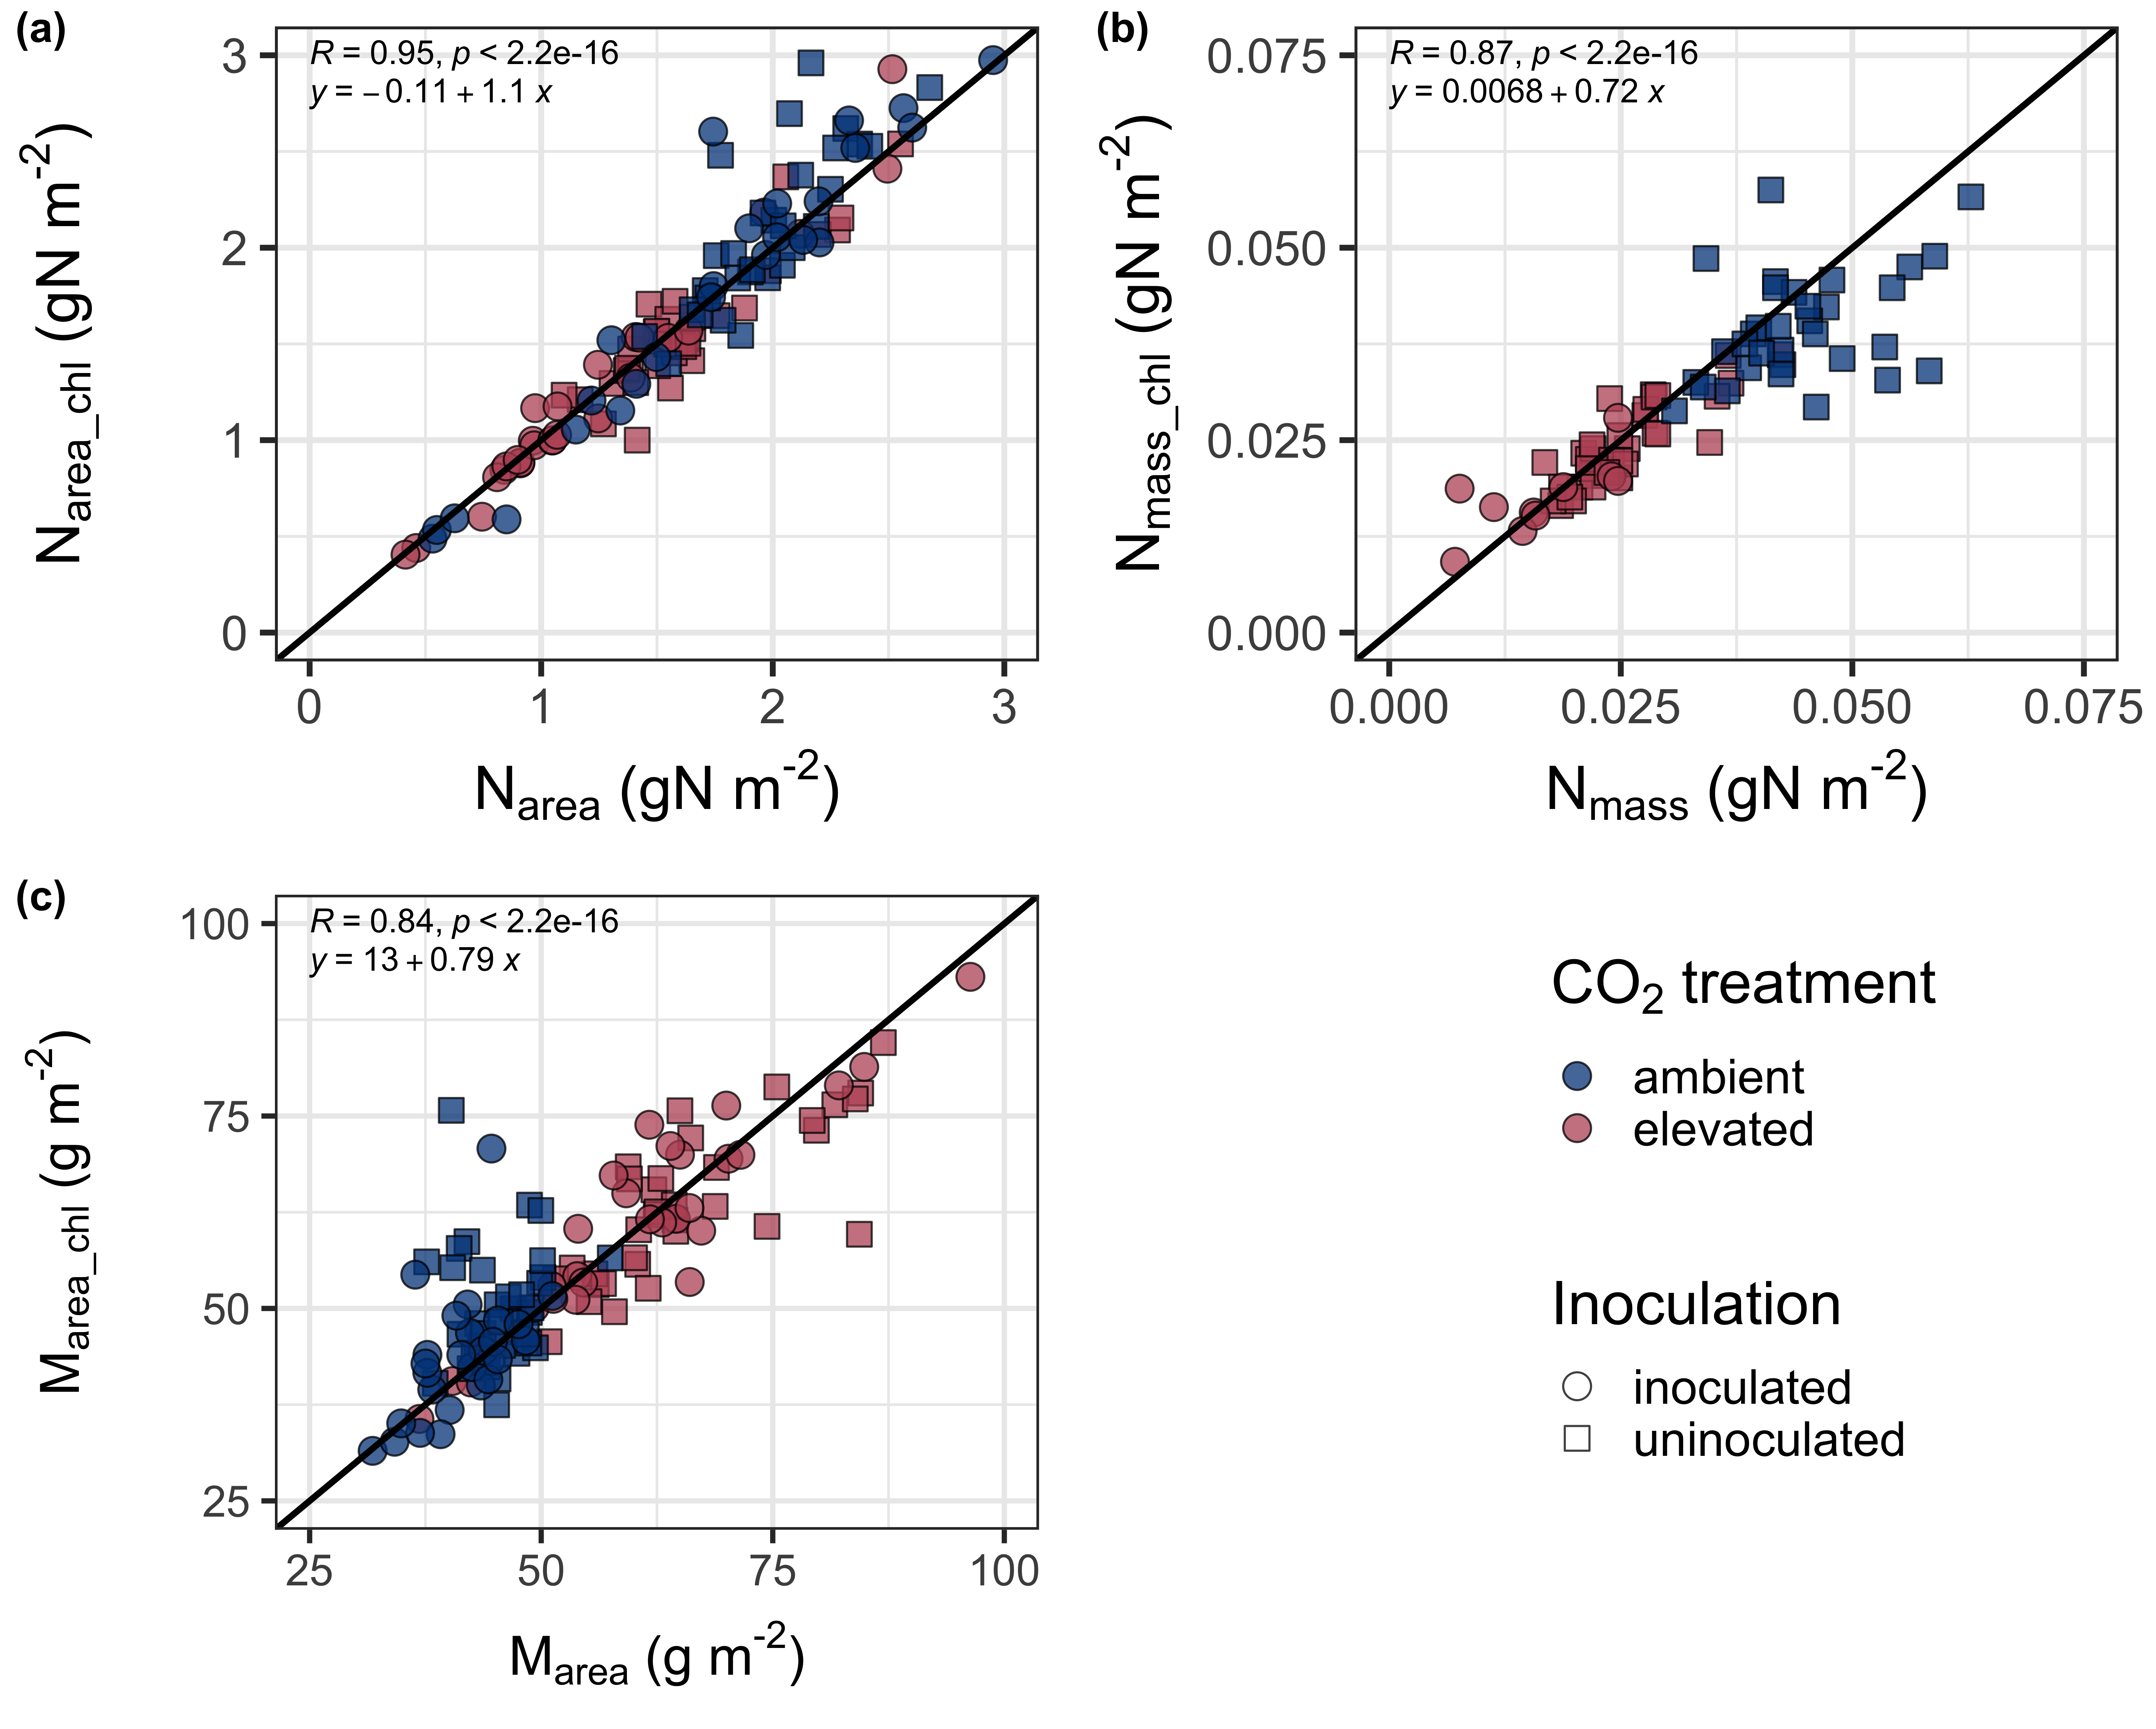
\includegraphics[scale = 0.0625]{ch5_NxCO2xI/figs/NxCO2xI_figS1_leafN_chl_.png}
    \caption[Relationships between area-based leaf nitrogen content, mass-based leaf nitrogen content, and leaf mass per unit leaf area measured on the focal leaf used to generate $A_\mathrm{net}$/$C_\mathrm{i}$ curves and leaf nitrogen content measured on the leaf used for chlorophyll extractions]{Relationships between area-based leaf nitrogen content (a), mass-based leaf nitrogen content (b), and leaf mass per unit leaf area (c) measured on the focal leaf used to generate $A_\mathrm{net}$/$C_\mathrm{i}$ curves and leaf nitrogen content measured on the leaf used for chlorophyll extractions. Blue points refer to leaves grown under ambient CO$_2$ and red points refer leaves grown under elevated CO$_2$. Square points indicate uninoculated pots and circular points indicate inoculated pots. Pearson's correlation, associated \textit{p}-values, and the line of the regression line that described each bivariate are included in the top left corner of each plot. The solid black line visualizes the trend given a 1:1 bivariate relationship.}
    \label{fig:figure.d1}
\end{figure}
\clearpage

\newpage
\begin{figure}
    \centering
    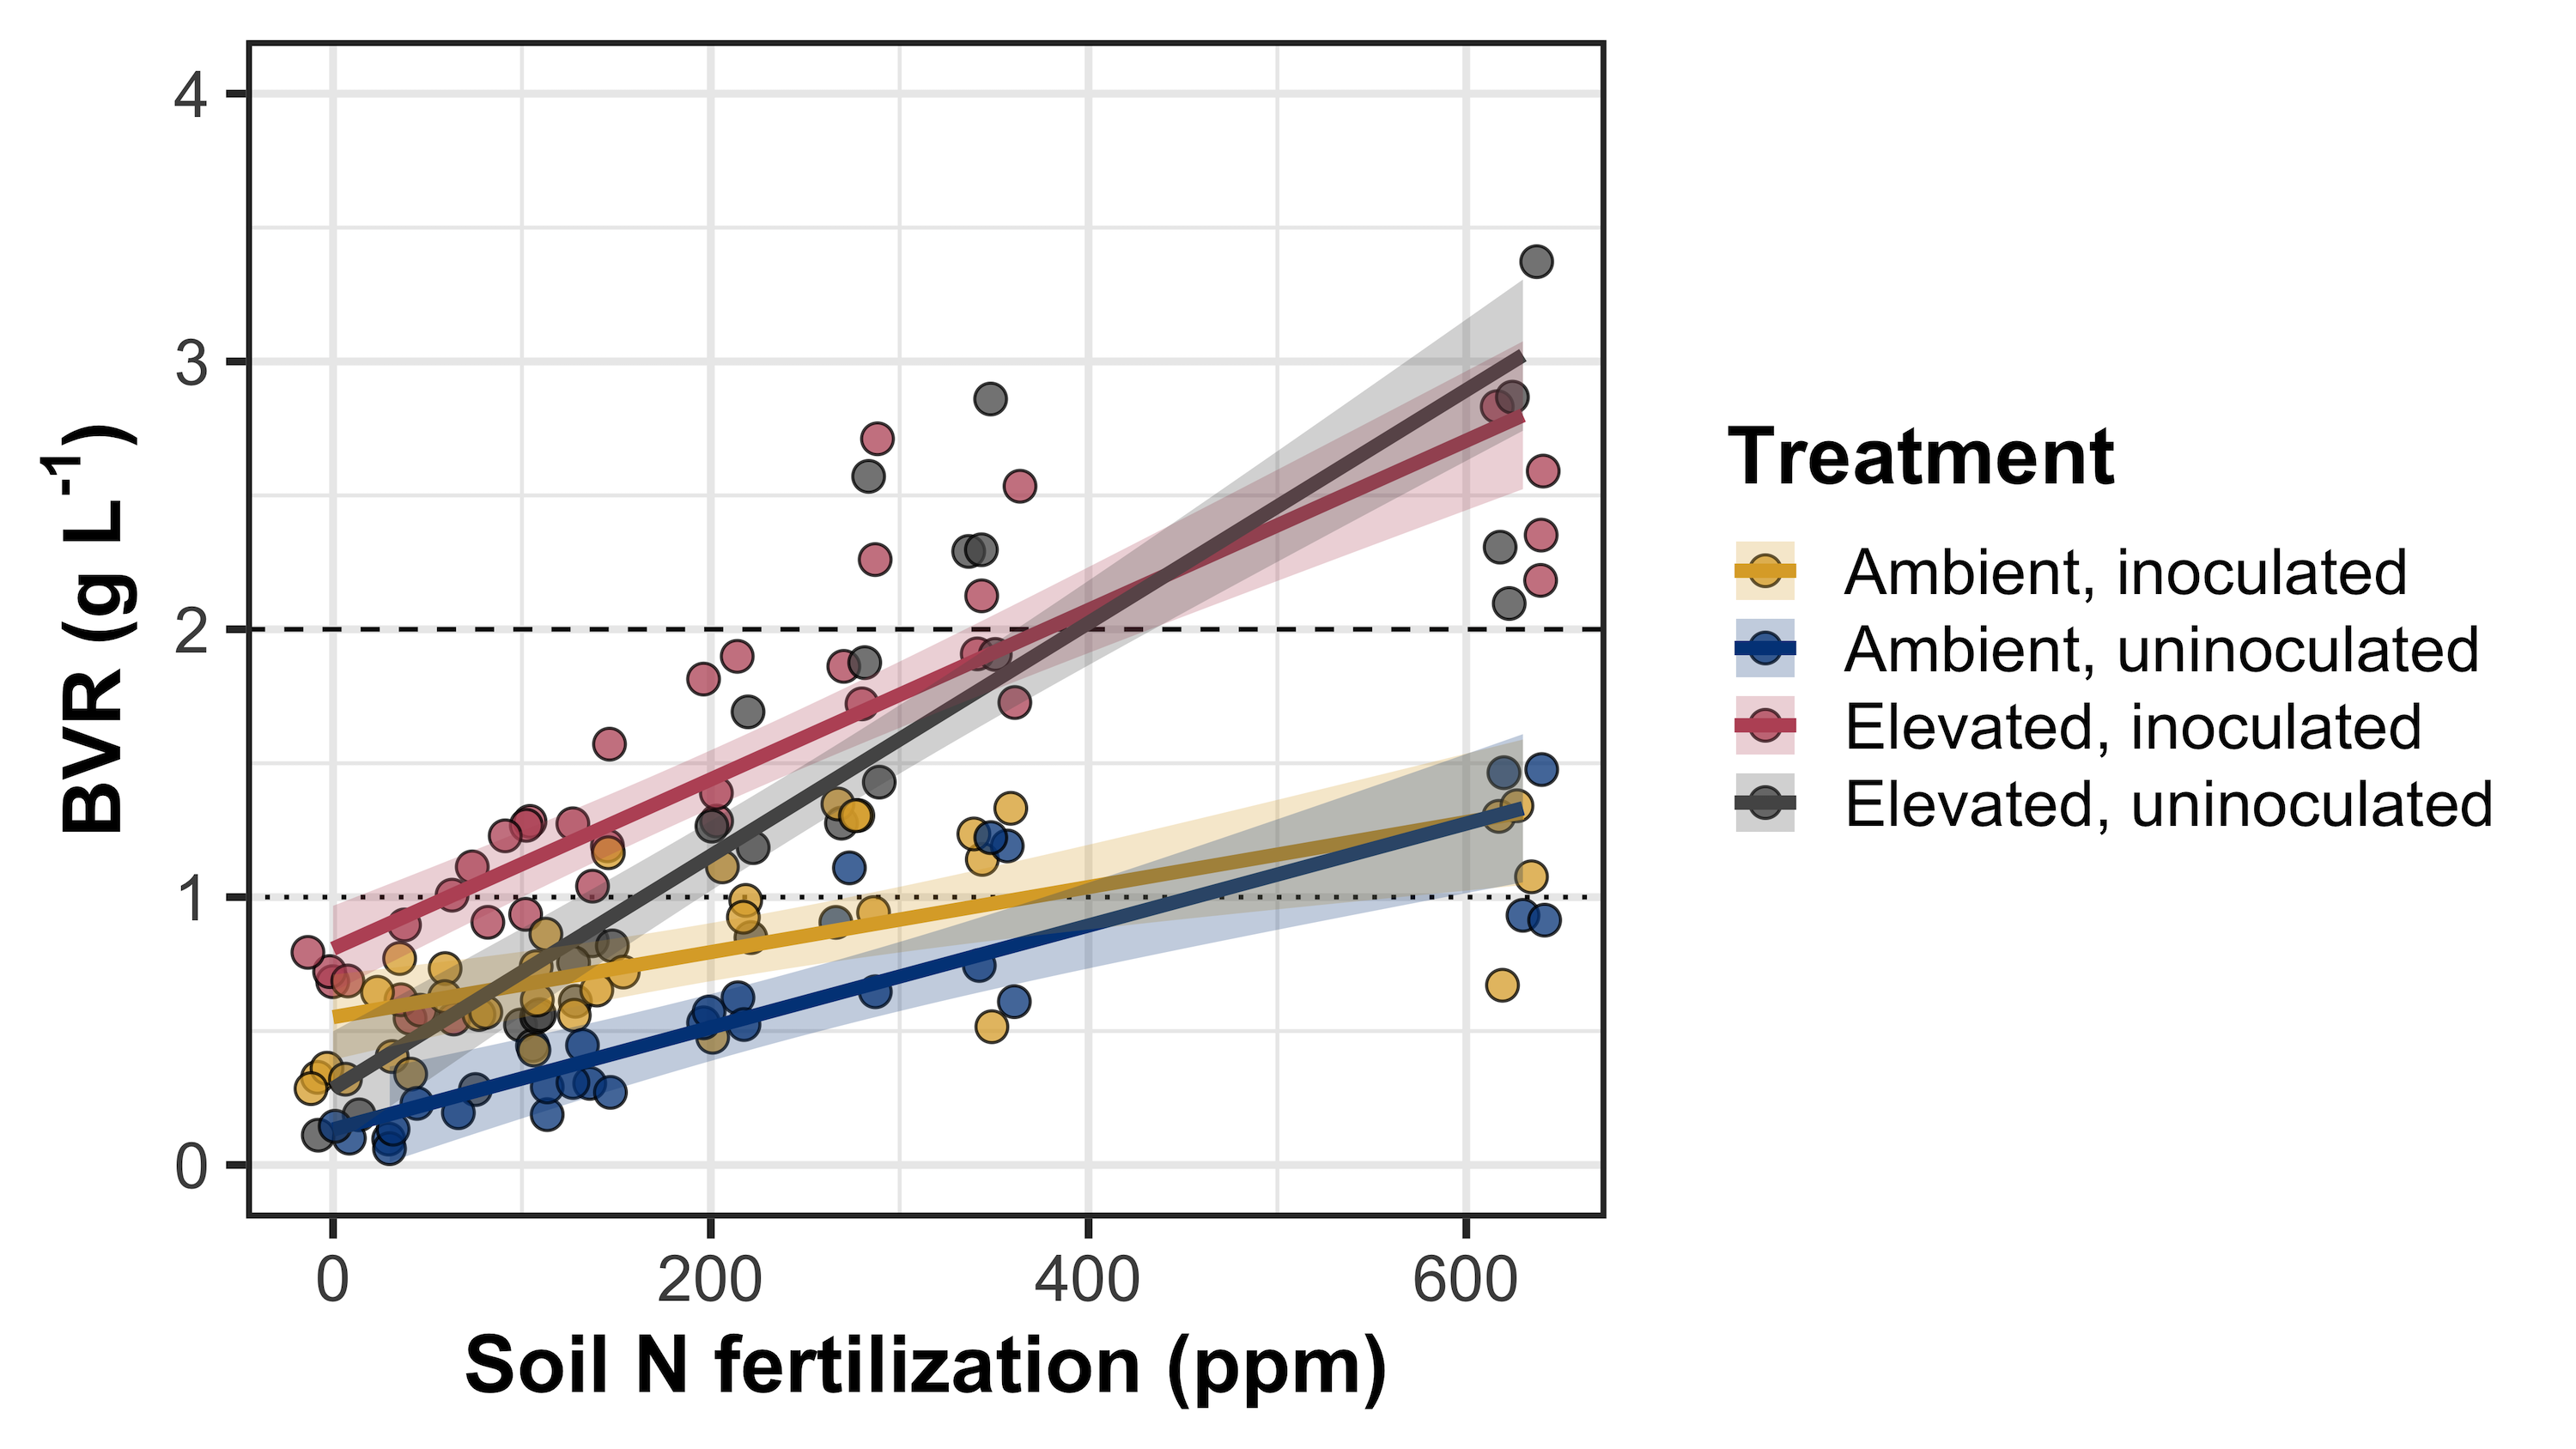
\includegraphics[scale = 0.07]{ch5_NxCO2xI/figs/NxCO2xI_figS2_bvr.png}
    \caption[Effects of CO$_2$, fertilization, and inoculation on the ratio of whole plant biomass to pot volume]{Effects of CO$_2$, fertilization, and inoculation on the ratio of whole plant biomass to pot volume. Soil nitrogen fertilization is represented on the x-axis in all panels. Yellow points and trendlines indicate inoculated individuals grown under ambient CO$_2$, blue points and trendlines indicate uninoculated individuals grown under ambient CO$_2$, red points and trendlines indicate inoculated individuals grown under elevated CO$_2$, and grey points indicate uninoculated individuals grown under elevated CO$_2$. Solid trendlines indicate regression slopes that are different from zero (\textit{p} < 0.05), while dashed trendlines indicate slopes that are not distinguishable from zero (\textit{p} > 0.05). The dotted horizontal line indicates the point where biomass:pot volume exceeds 1 g L$^{-1}$, and the dashed line indicates the point where biomass:pot volume exceeds 2 g L$^{-1}$.}
    \label{fig:figure.d2}
\end{figure}
\clearpage


%%%%%%%%%%%%%%%%%%%%%%%%%%%%%%%%%%%%%%%%%%%%%%%%%%%%%%%%
%End document
%%%%%%%%%%%%%%%%%%%%%%%%%%%%%%%%%%%%%%%%%%%%%%%%%%%%%%%%
\end{document}